\documentclass[openright,twoside,11pt]{book}
  % Index.  Must be before loading hyperref.
  \usepackage{myindex}
  \usepackage{index}
  \makeindex
  \usepackage{urbi-report}
  \usepackage{indexing}
  \usepackage{revision}

% CONFIGURATION
\title{The Urbi Software Development Kit}
\subtitle{Version \VcsDescription}
\author{Kernel Team}

% DOCUMENT
\begin{document}

\maketitle
\tableofcontents

%% Copyright (C) 2009-2011, Gostai S.A.S.
%%
%% This software is provided "as is" without warranty of any kind,
%% either expressed or implied, including but not limited to the
%% implied warranties of fitness for a particular purpose.
%%
%% See the LICENSE file for more information.

\chapter{Introduction}

\usdk is a fully-featured environment to orchestrate complex
organizations of components.  It relies on a middleware architecture
that coordinates components named UObjects.  It also features \us, a
scripting language that can be used to write orchestration programs.

\section{\urbi and UObjects}

\urbi makes the orchestration of independent, concurrent, components easier.
It was first designed for robotics: it provides all the needed features to
coordinate the execution of various components (actuators, sensors, software
devices that provide features such as text-to-speech, face recognition and
so forth).  Languages such as \Cxx are well suited to program the local,
low-level, handling of these hardware or software devices; indeed one needs
efficiency, small memory footprint, and access to low-level hardware
details.  Yet, when it comes to component orchestration and coordination, in
a word, when it comes to addressing concurrency, it can be tedious to use
such languages.

Middleware infrastructures make possible to use remote components as if they
were local, to allow concurrent execution, to make synchronous or
asynchronous requests and so forth.  The \dfn{UObject} \Cxx architecture
provides exactly this: a common API that allows conforming components to be
used seamlessly in highly concurrent settings.  Components need not be
designed with UObjects in mind, rather, UObjects are typically ``shells''
around ``regular'' components.

Components with an UObject interface are naturally supported by the \us
programming language.  This provides a tremendous help: one can interact
with these components (making queries, changing them, observing their state,
monitoring various kinds of events and so forth), which provides a huge
speed-up during development.

Although made with robots in mind, the UObject architecture is well suited
to tame any heavily concurrent environment, such as video games or complex
systems in general.

\section{The Big Picture}

The \autoref{fig:arch} shows the architecture of \urbi.  Let's browse it
bottom up.

\begin{figure}[p]
  \centering
  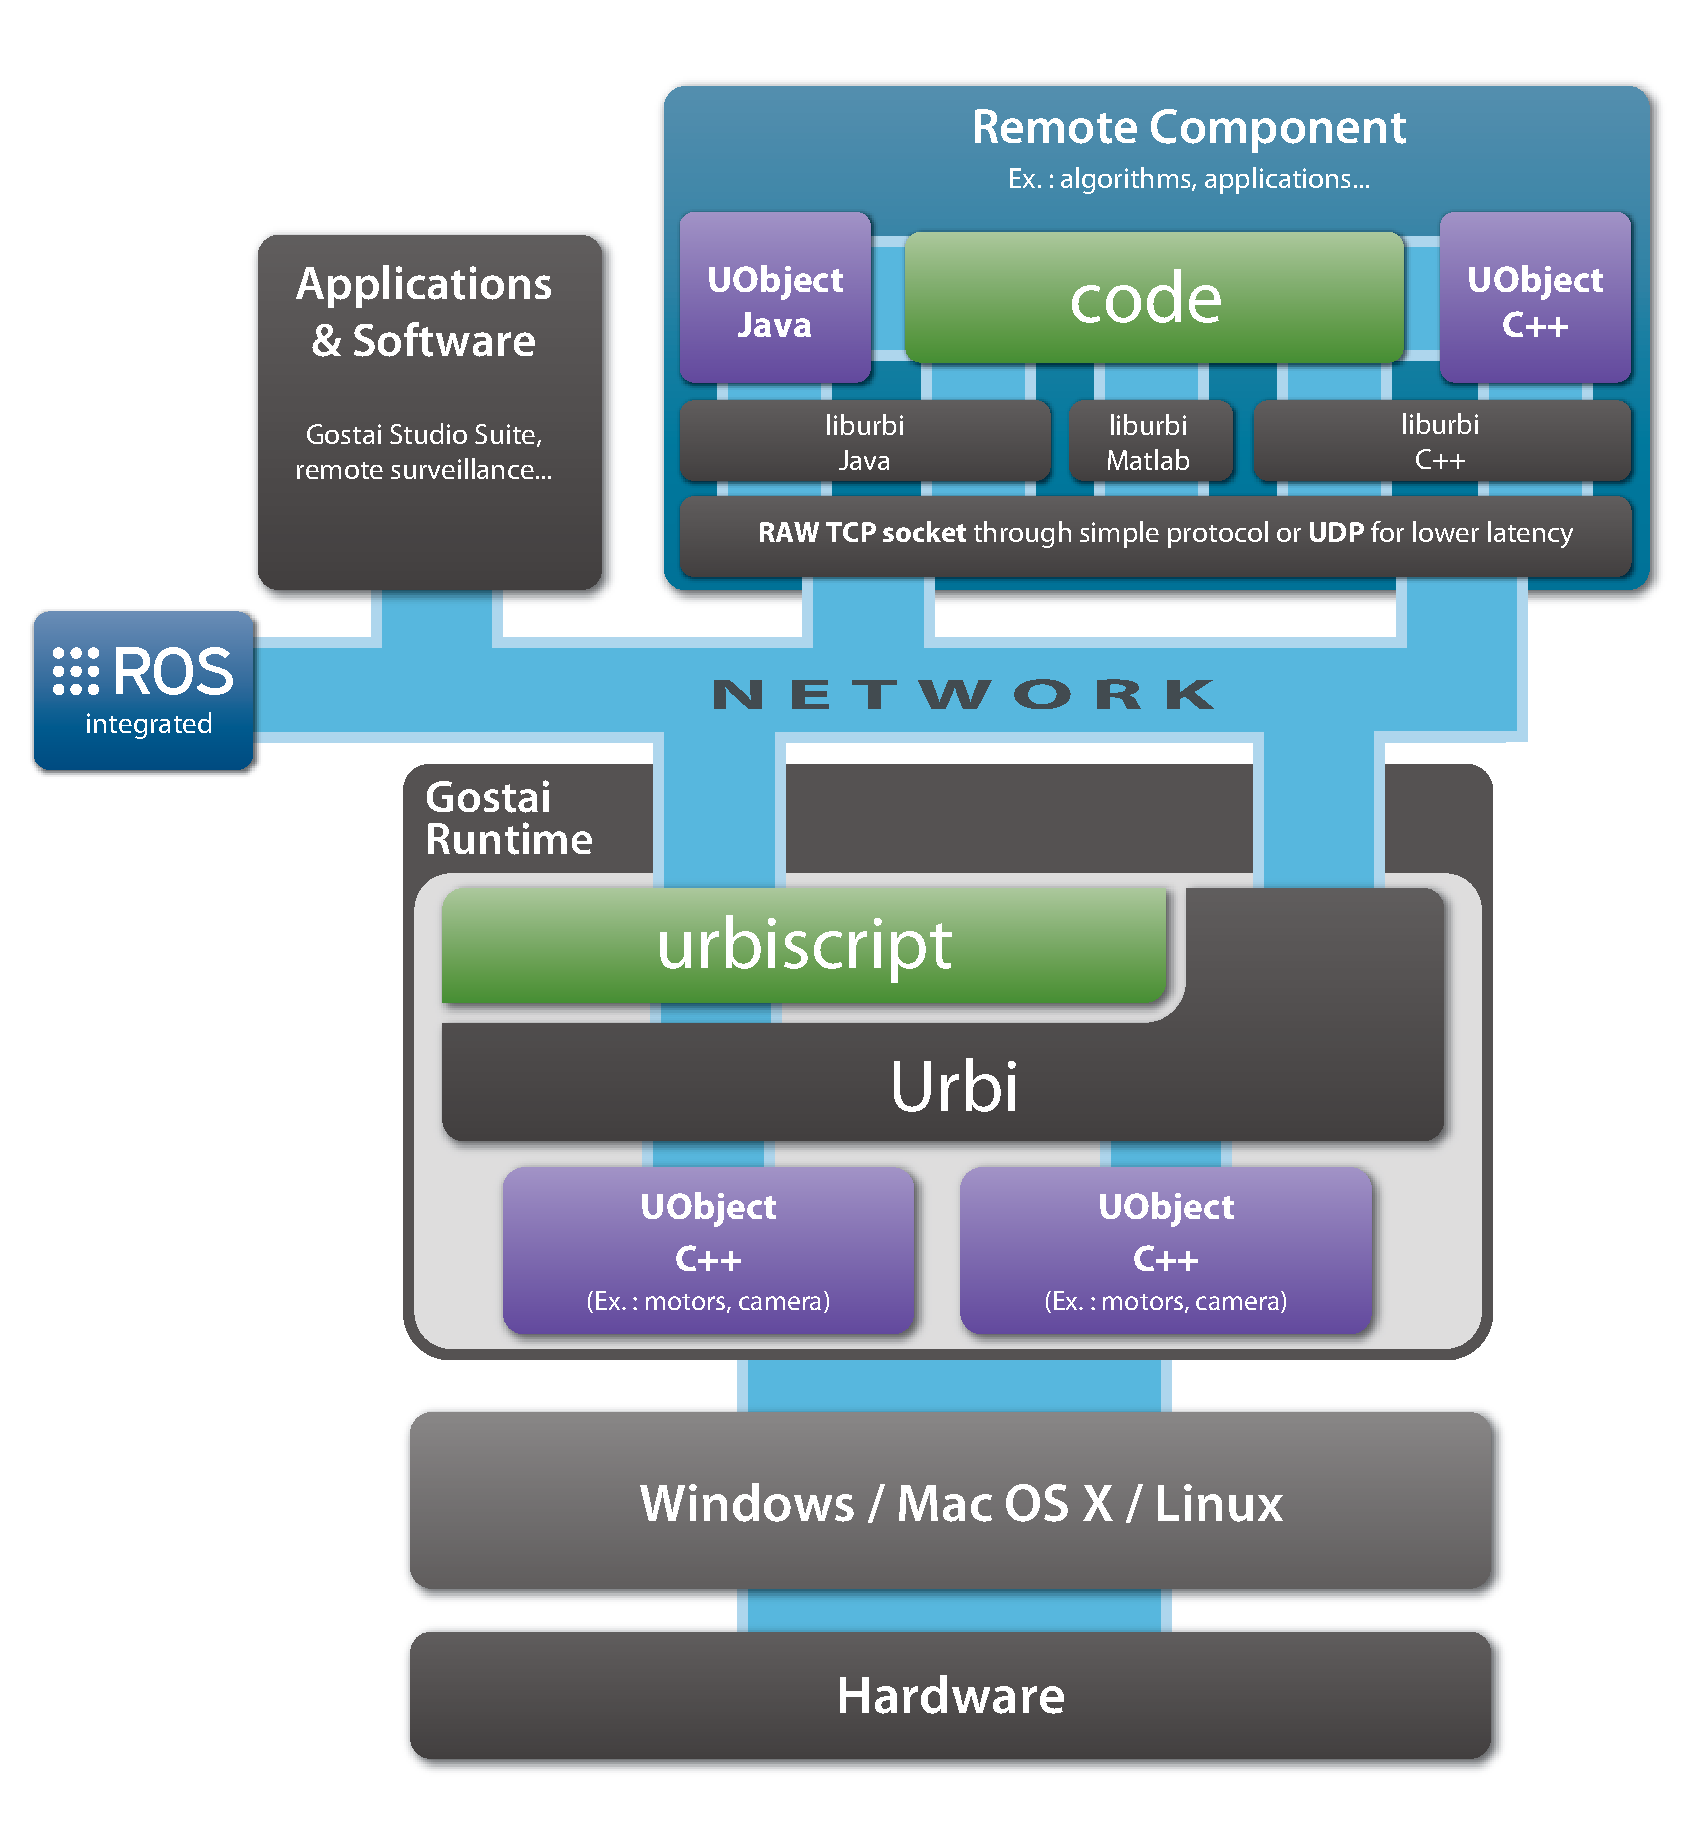
\includegraphics[width=.8\linewidth]{img/urbi-architecture}
  \caption{A Bird-View of the \urbi Architecture}
  \label{fig:arch}
\end{figure}

At the lowest level, \urbi requires a (possibly very limited) embedded
computer.  This is the case for most robots today, but on occasion, some
device cannot even run reasonably small pieces of code.  In that case, \urbi
can still be used, but then the robot is actually remote-controled from a
computer running \urbi.

Right on top of the hardware, is running the \dfn{Operating System}.  \urbi
supports the major OSes; it was also ported on top of realtime OSes such as
Xenomai, and on specific OSes such as Aperios, Sony's proprietary system
running its Aibo robotic dog.

The \dfn{Urbi Runtime}, which is the actual core of the system, also known
as the \dfn{engine} or the \dfn{kernel}, is interfacing the OS with the rest
of the \urbi world, \us and UObjects.

UObjects are used to bind hardware or software components, such as
actuators and sensors on the one hand, and voice synthesis or face
recognition on the other hand.  They can be run locally on the robot, or on
a remote, more powerful, computer.

To orchestrate all the components, \us is a programming language of choice
(see below).

Finally, applications are available for the \urbi environment.  For
instance, Gostai Studio provides high-level tools to develop complex robotic
behaviors.

\section{\urbi and \us}

\us is a programming language primarily designed for robotics. It's a
dynamic, prototype-based, object-oriented scripting language. It supports
and emphasizes parallel and event-based programming, which are very popular
paradigms in robotics, by providing core primitives and language constructs.

\medskip

Its main features are:
\begin{itemize}
\item syntactically close to \Cxx.\\
  If you know \C, \Cxx, \Java, or JavaScript, you can easily write \us
  programs.
\item fully integrated with \Cxx.\\
  You can bind \Cxx classes in \us seamlessly. \us is also integrated with
  many other languages such as \Java, \MatLab or \Python.
\item object-oriented.\\
  It supports encapsulation, inheritance and inclusion polymorphism. Dynamic
  dispatching is available through monomethods --- just as \Cxx, \Cs or
  \Java.
\item concurrent.\\
  It provides you with natural constructs to run and control high numbers of
  interacting concurrent tasks.
\item event-based.\\
  Triggering events and reacting to them is absolutely straightforward.
\item functional programming.\\
  Inspired by languages such as \Lisp or \Caml, \us features first class
  functions and pattern matching.
\item client/server.\\
  The interpreter accepts multiple connections from different sources (human
  users, robots, other servers \ldots) and enables them to interact.
\item distributed.\\
  You can run objects in different processes, potentially remote computers
  across the network.
\end{itemize}

\section{Genesis}

\urbi what first designed and implemented by Jean-Christophe Baillie,
together with Matthieu Nottale.  Because its users wildly acclaimed it,
Jean-Christophe founded Gostai, a France-based Company that develops
software for robotics with a strong emphasis on personal robotics.

\paragraph{Authors}
\usdk 1 was further developed by Akim Demaille, Guillaume Deslandes, Quentin
Hocquet, and Benoît Sigoure.

The \usdk 2 project was started and developed by Akim Demaille, Quentin
Hocquet, Matthieu Nottale, and Benoît Sigoure.  Samuel Tardieu provided an
immense help during the year 2008, in particular for the concurrency and
event support.

The maintenance is currently carried out by Akim Demaille, Quentin
Hocquet, and Matthieu Nottale.  Jean-Christophe Baillie is still
deeply involved in the development of \us, he regularly submits ideas,
and occasionally even code!

\paragraph{Contributors}

A number of people contributed significantly to \urbi, including Romain
Bezut, Thomas Moulard, Clément Moussu, Nicolas Pierron.

\section{Outline}

This multi-part document provides a complete guide to Urbi.  See
\autoref{sec:notations} for the various notations that are used in the
document.

\newenvironment{partDescription}[2]
{%
  \item[\autoref{#1} --- \nameref{#1}]~\\%
  #2
  \begin{description}%
    \let\itemOrig\item%
    \renewcommand{\item}[1][]{\itemOrig[~~\autoref{##1} --- \nameref{##1}]~\\}%
  }{%
  \end{description}%
}

%%% Keep sync with urbi-sdk.tex.
\begin{description}
%% Copyright (C) 2010, Gostai S.A.S.
%%
%% This software is provided "as is" without warranty of any kind,
%% either expressed or implied, including but not limited to the
%% implied warranties of fitness for a particular purpose.
%%
%% See the LICENSE file for more information.

\begin{partDescription}{part:tut}
  {%
    This part, also known as the ``\us tutorial'', teaches the reader
    how to program in
    \us.  It goes from the basis to concurrent and
    event-based programming.  No specific knowledge is expected.
    There is no need for a \Cxx compiler, as \UObject will not be
    covered here (see \autoref{part:uobject}).  The reference manual
    contains a terse and complete definition of the \urbi environment
    (\autoref{part:specs}).
    %
  }
\item[sec:tut:first]
  First contacts with \us.
\item[sec:tut:value]
  A quick introduction to objects and values.
\item[sec:tut:flow]
  Basic control flow: \lstinline{if}, \lstinline{for} and the like.
\item[sec:tut:function]
  Details about functions, scoped, and lexical closures.
\item[sec:tut:object]
  A more in-depth introduction to object-oriented programming in \us.
\item[sec:tut:functional]
  Functions are first-class citizens.
\item[sec:tut:concurrent]
  The \us operators for concurrency, tags.
\item[sec:tut:event-prog]
  Support for event-driven concurrency in \us.
\item[sec:tut:ros] How to use ROS from \urbi, and vice-versa.
\end{partDescription}


%%% Local Variables:
%%% mode: latex
%%% TeX-master: "../urbi-sdk"
%%% ispell-dictionary: "american"
%%% ispell-personal-dictionary: "../urbi.dict"
%%% fill-column: 76
%%% End:

%% Copyright (C) 2010, Gostai S.A.S.
%%
%% This software is provided "as is" without warranty of any kind,
%% either expressed or implied, including but not limited to the
%% implied warranties of fitness for a particular purpose.
%%
%% See the LICENSE file for more information.

\begin{partDescription}{part:tut}
  {%
    This part, also known as the ``\us tutorial'', teaches the reader
    how to program in
    \us.  It goes from the basis to concurrent and
    event-based programming.  No specific knowledge is expected.
    There is no need for a \Cxx compiler, as \UObject will not be
    covered here (see \autoref{part:uobject}).  The reference manual
    contains a terse and complete definition of the \urbi environment
    (\autoref{part:specs}).
    %
  }
\item[sec:tut:first]
  First contacts with \us.
\item[sec:tut:value]
  A quick introduction to objects and values.
\item[sec:tut:flow]
  Basic control flow: \lstinline{if}, \lstinline{for} and the like.
\item[sec:tut:function]
  Details about functions, scoped, and lexical closures.
\item[sec:tut:object]
  A more in-depth introduction to object-oriented programming in \us.
\item[sec:tut:functional]
  Functions are first-class citizens.
\item[sec:tut:concurrent]
  The \us operators for concurrency, tags.
\item[sec:tut:event-prog]
  Support for event-driven concurrency in \us.
\item[sec:tut:ros] How to use ROS from \urbi, and vice-versa.
\end{partDescription}


%%% Local Variables:
%%% mode: latex
%%% TeX-master: "../urbi-sdk"
%%% ispell-dictionary: "american"
%%% ispell-personal-dictionary: "../urbi.dict"
%%% fill-column: 76
%%% End:

%% Copyright (C) 2010, Gostai S.A.S.
%%
%% This software is provided "as is" without warranty of any kind,
%% either expressed or implied, including but not limited to the
%% implied warranties of fitness for a particular purpose.
%%
%% See the LICENSE file for more information.

\begin{partDescription}{part:tut}
  {%
    This part, also known as the ``\us tutorial'', teaches the reader
    how to program in
    \us.  It goes from the basis to concurrent and
    event-based programming.  No specific knowledge is expected.
    There is no need for a \Cxx compiler, as \UObject will not be
    covered here (see \autoref{part:uobject}).  The reference manual
    contains a terse and complete definition of the \urbi environment
    (\autoref{part:specs}).
    %
  }
\item[sec:tut:first]
  First contacts with \us.
\item[sec:tut:value]
  A quick introduction to objects and values.
\item[sec:tut:flow]
  Basic control flow: \lstinline{if}, \lstinline{for} and the like.
\item[sec:tut:function]
  Details about functions, scoped, and lexical closures.
\item[sec:tut:object]
  A more in-depth introduction to object-oriented programming in \us.
\item[sec:tut:functional]
  Functions are first-class citizens.
\item[sec:tut:concurrent]
  The \us operators for concurrency, tags.
\item[sec:tut:event-prog]
  Support for event-driven concurrency in \us.
\item[sec:tut:ros] How to use ROS from \urbi, and vice-versa.
\end{partDescription}


%%% Local Variables:
%%% mode: latex
%%% TeX-master: "../urbi-sdk"
%%% ispell-dictionary: "american"
%%% ispell-personal-dictionary: "../urbi.dict"
%%% fill-column: 76
%%% End:

%% Copyright (C) 2010, Gostai S.A.S.
%%
%% This software is provided "as is" without warranty of any kind,
%% either expressed or implied, including but not limited to the
%% implied warranties of fitness for a particular purpose.
%%
%% See the LICENSE file for more information.

\begin{partDescription}{part:tut}
  {%
    This part, also known as the ``\us tutorial'', teaches the reader
    how to program in
    \us.  It goes from the basis to concurrent and
    event-based programming.  No specific knowledge is expected.
    There is no need for a \Cxx compiler, as \UObject will not be
    covered here (see \autoref{part:uobject}).  The reference manual
    contains a terse and complete definition of the \urbi environment
    (\autoref{part:specs}).
    %
  }
\item[sec:tut:first]
  First contacts with \us.
\item[sec:tut:value]
  A quick introduction to objects and values.
\item[sec:tut:flow]
  Basic control flow: \lstinline{if}, \lstinline{for} and the like.
\item[sec:tut:function]
  Details about functions, scoped, and lexical closures.
\item[sec:tut:object]
  A more in-depth introduction to object-oriented programming in \us.
\item[sec:tut:functional]
  Functions are first-class citizens.
\item[sec:tut:concurrent]
  The \us operators for concurrency, tags.
\item[sec:tut:event-prog]
  Support for event-driven concurrency in \us.
\item[sec:tut:ros] How to use ROS from \urbi, and vice-versa.
\end{partDescription}


%%% Local Variables:
%%% mode: latex
%%% TeX-master: "../urbi-sdk"
%%% ispell-dictionary: "american"
%%% ispell-personal-dictionary: "../urbi.dict"
%%% fill-column: 76
%%% End:

\ifthen{\boolean{platforms}}
{
  %% Copyright (C) 2010, Gostai S.A.S.
%%
%% This software is provided "as is" without warranty of any kind,
%% either expressed or implied, including but not limited to the
%% implied warranties of fitness for a particular purpose.
%%
%% See the LICENSE file for more information.

\begin{partDescription}{part:tut}
  {%
    This part, also known as the ``\us tutorial'', teaches the reader
    how to program in
    \us.  It goes from the basis to concurrent and
    event-based programming.  No specific knowledge is expected.
    There is no need for a \Cxx compiler, as \UObject will not be
    covered here (see \autoref{part:uobject}).  The reference manual
    contains a terse and complete definition of the \urbi environment
    (\autoref{part:specs}).
    %
  }
\item[sec:tut:first]
  First contacts with \us.
\item[sec:tut:value]
  A quick introduction to objects and values.
\item[sec:tut:flow]
  Basic control flow: \lstinline{if}, \lstinline{for} and the like.
\item[sec:tut:function]
  Details about functions, scoped, and lexical closures.
\item[sec:tut:object]
  A more in-depth introduction to object-oriented programming in \us.
\item[sec:tut:functional]
  Functions are first-class citizens.
\item[sec:tut:concurrent]
  The \us operators for concurrency, tags.
\item[sec:tut:event-prog]
  Support for event-driven concurrency in \us.
\item[sec:tut:ros] How to use ROS from \urbi, and vice-versa.
\end{partDescription}


%%% Local Variables:
%%% mode: latex
%%% TeX-master: "../urbi-sdk"
%%% ispell-dictionary: "american"
%%% ispell-personal-dictionary: "../urbi.dict"
%%% fill-column: 76
%%% End:

}
%% Copyright (C) 2010, Gostai S.A.S.
%%
%% This software is provided "as is" without warranty of any kind,
%% either expressed or implied, including but not limited to the
%% implied warranties of fitness for a particular purpose.
%%
%% See the LICENSE file for more information.

\begin{partDescription}{part:tut}
  {%
    This part, also known as the ``\us tutorial'', teaches the reader
    how to program in
    \us.  It goes from the basis to concurrent and
    event-based programming.  No specific knowledge is expected.
    There is no need for a \Cxx compiler, as \UObject will not be
    covered here (see \autoref{part:uobject}).  The reference manual
    contains a terse and complete definition of the \urbi environment
    (\autoref{part:specs}).
    %
  }
\item[sec:tut:first]
  First contacts with \us.
\item[sec:tut:value]
  A quick introduction to objects and values.
\item[sec:tut:flow]
  Basic control flow: \lstinline{if}, \lstinline{for} and the like.
\item[sec:tut:function]
  Details about functions, scoped, and lexical closures.
\item[sec:tut:object]
  A more in-depth introduction to object-oriented programming in \us.
\item[sec:tut:functional]
  Functions are first-class citizens.
\item[sec:tut:concurrent]
  The \us operators for concurrency, tags.
\item[sec:tut:event-prog]
  Support for event-driven concurrency in \us.
\item[sec:tut:ros] How to use ROS from \urbi, and vice-versa.
\end{partDescription}


%%% Local Variables:
%%% mode: latex
%%% TeX-master: "../urbi-sdk"
%%% ispell-dictionary: "american"
%%% ispell-personal-dictionary: "../urbi.dict"
%%% fill-column: 76
%%% End:

\end{description}

%% Redefine this environment so that next time the */abstract.tex
%% files are read, they create the part instead of referencing to it.

\renewenvironment{partDescription}[2]
{%
  \chapter*{About This Part}
  #2
  \begin{description}%
    \let\itemOrig\item%
    \renewcommand{\item}[1][]{\itemOrig[~~\autoref{##1} --- \nameref{##1}]~\\}%
  }{%
  \end{description}%
}


%%% Local Variables:
%%% mode: latex
%%% TeX-master: "urbi-sdk"
%%% ispell-dictionary: "american"
%%% ispell-personal-dictionary: "urbi.dict"
%%% fill-column: 76
%%% End:


\part{Urbi SDK Tutorial}
\chapter{Getting started}

\us comes with a set of tools, two of which being of particular
importance:
\begin{description}
\item[\dfn{urbi}] launches an \urbi server.  There are several means
  to interact with this server, which will see later.
\item[\dfn{urbi-launch}] runs \urbi components, the UObjects, and connects
  them to an \urbi server.
\end{description}

Please, first make sure that these tools are properly installed.  If
you encounter problems, please see \autoref{sec:installation}, which
is more detailed, and possibly \autoref{sec:faq} for frequently asked
questions.

\begin{shell}
# Make sure urbi is properly installed.
$ urbi --version
Urbi Kernel version preview/2.0/beta3-425 rev. 000913e
Copyright (C) 2005-2009 Gostai SAS.

URBI SDK Remote version preview/1.6/beta1-666 rev. 92ec3b4
Copyright (C) 2004-2009 Gostai SAS.

Libport version preview/1.0/beta1-1048 rev. f1c5170
Copyright (C) 2005-2009 Gostai SAS.
\end{shell}%$


There are several means to interact with a server spawned by
\command{urbi}.  First of all, you may use the options
\option{-e}/\option{--expression \var{code}} and
\option{-f}/\option{--file \var{file}} to send some \var{code} or the
contents of some \var{file} to the newly run server.  You may combine
any number of these options, but beware that being event-driven, the
server does not ``know'' when a program ends.  Therefore, batch
programs should end by calling \code{shutdown}:

\begin{shell}
# A classical program.
$ urbi -e 'echo("Hello, World!");' -e 'shutdown;'
[00000004] *** Hello, World!
\end{shell}%$

To run an interactive session, use option
\option{-i}/\option{--interactive}.  Like most interactive
interpreters, \urbi will evaluate the given commands and print out the
results.

\begin{shell}
$ urbi -i
[00000000:start] *** **********************************************************
[00000000:start] *** Urbi Kernel version preview/2.0/beta3-425 rev. 000913e
[00000000:start] *** Copyright (C) 2005-2009 Gostai SAS.
[00000000:start] ***
[00000000:start] *** URBI SDK Remote version preview/1.6/beta1-666 rev. 92ec3b4
[00000000:start] *** Copyright (C) 2004-2009 Gostai SAS.
[00000000:start] ***
[00000000:start] *** Libport version preview/1.0/beta1-1048 rev. f1c5170
[00000000:start] *** Copyright (C) 2005-2009 Gostai SAS.
[00000000:start] ***
[00000000:start] *** URBI comes with ABSOLUTELY NO WARRANTY.
[00000000:start] *** This software can be used under certain conditions;
[00000000:start] *** see LICENSE file for details.
[00000000:start] ***
[00000000:start] *** See http://www.urbiforge.com for news and updates.
[00000000:start] *** **********************************************************
[00000000:start] ***
[00000000:ident] *** ID: U3154688
[00000004:start] *** Urbi is up and running.
1+2;
[00000006] 3
shutdown;
\end{shell}%$

The output from the server is prefixed by a number surrounded by
square brackets: this is the date (in milliseconds since the server
was launched) at which that line was sent by the server. This is
useful at occasions, since \urbi is meant to run many parallel
commands.  But since these timestamps are irrelevant in most examples,
they will often be filled with zeroes through this documentation.

The program \command{rlwrap} provides additional services (history of
commands, advanced command line edition etc.); run \samp{rlwrap
  urbi -i}.

In either case the server can also be made available for network-based
interactions using option \option{--port \var{port}}.  Note that while
\code{shutdown} terminates the server, \code{quit} only terminates one
interactive session.  In the following example the server is still
available for other, possibly concurrent, sessions.

\begin{shell}
$ urbi --port 54000 &
[1] 77024
$ telnet localhost 54000
Trying 127.0.0.1...
Connected to localhost.
Escape character is '^]'.
[00000758:start] *** **********************************************************
[00000758:start] *** Urbi Kernel version preview/2.0/beta3-425 rev. 000913e
[00000758:start] *** Copyright (C) 2005-2009 Gostai SAS.
[00000758:start] ***
[00000758:start] *** URBI SDK Remote version preview/1.6/beta1-666 rev. 92ec3b4
[00000758:start] *** Copyright (C) 2004-2009 Gostai SAS.
[00000758:start] ***
[00000758:start] *** Libport version preview/1.0/beta1-1048 rev. f1c5170
[00000758:start] *** Copyright (C) 2005-2009 Gostai SAS.
[00000758:start] ***
[00000758:start] *** URBI comes with ABSOLUTELY NO WARRANTY.
[00000758:start] *** This software can be used under certain conditions;
[00000758:start] *** see LICENSE file for details.
[00000758:start] ***
[00000758:start] *** See http://www.urbiforge.com for news and updates.
[00000758:start] *** **********************************************************
[00000758:start] ***
[00000758:ident] *** ID: U348160
12345679*8;
[00018032] 98765432
quit;
\end{shell}%$

The program \command{urbi-send} provides a nice interface to
interact with a running server.

\begin{shell}
$ urbi-send -p 54000 -e '1+2*3;' -e 'quit;'
[00018032:] 7
# Have the server shutdown;
$ urbi-send -p 54000 -e 'shutdown;'
\end{shell}

\medskip

You can now send commands to your \urbi server. If at any point you
get lost, or want a fresh start, you can simply close and reopen your
connection to the server to get a clean environment.  In some cases,
particularly if you made global changes in the environment, it is
simpler start anew: shutdown your current server, and spawn a new one.

\chapter{First steps}

This section intends to provide the most basic notions to write \us
code. Some aspects are presented only superficially. The point of this
section is to bootstrap yourself with the \us language, to be able
to study more in-depth examples afterwards.

\section{Comments\index{comment}}

Commenting your code is crucial, so let's start by learning how to do
this in \us. Comments are ignored by the interpreter, and
can be left as documentation, reminder, \ldots \us supports \C and
\Cxx style style comments (\autoref{lst:tut:comments}):

\begin{itemize}
\item \C style comments start with \texttt{/*} and end with \texttt{*/}.
\item \Cxx style comments start with \texttt{//} and last until the
  end of the line.
\end{itemize}


\begin{urbiscript}[caption=Comments in \us, label=lst:tut:comments]
1; // This is a C++ style comment.
[00000000] 1
2 + /* This is a C-style comment. */ 2;
[00000000] 4
/* Contrary to C/C++, this type of comment /* does nest */. */
3;
[00000000] 3
\end{urbiscript}


\section{Literal values}

As already seen, we can evaluate literal integers. \us supports
several other literals, such as:

\begin{description}
\item[floats] floating point numbers.
\item[strings] character strings.
\item[lists] ordered collection of values.
\item[nil] neutral value. Think of it as the value that fits anywhere.
\item[void] absence of value. Think of it as the value that fits nowhere.
\end{description}

These literal values can be obtained with the syntax presented in
\autoref{lst:tut:literals}.

\begin{urbiscript}[caption=Literals,label=lst:tut:literals]
42; // Integer literal.
[00000000] 42
3.14; // Floating point number literal.
[00000000] 3.14
"string"; // Character string literal.
[00000000] "string"
[1, 2, "a", "b"]; // List literal.
[00000000] [1, 2, "a", "b"]
nil;
void;
\end{urbiscript}

Listing \ref{lst:tut:literals} highlights some point:
\begin{itemize}
\item Lists in \us are heterogeneous. That is, one list can hold
  values of different types.
\item The printing of nil and void is empty.
\end{itemize}

\section{Function calls}

You can call functions with the classical, mathematical notation
(\autoref{lst:tut:calling-functions}).

\begin{urbiscript}[caption=Calling functions,label=lst:tut:calling-functions]
cos(0); // Compute cosinus
[00000000] 1
max(1, 3); // Get the maximum of the arguments.
[00000000] 3
max(1, 3, 4, 2);
[00000000] 4
\end{urbiscript}

Again, the result of the evaluation are printed out. You can see here
that function in \us can be variadic, that is, take different number
of arguments, such as the \lstinline{max} function. Let's now try the
\lstinline{echo} function, that prints out its argument
(\autoref{lst:tut:printing}).

\begin{urbiscript}[caption=Printing out,label=lst:tut:printing]
echo("Hello world!");
[00000000] *** Hello world!
\end{urbiscript}

The server prints out \lstinline{Hello world!}, as expected. Note that
this output is still prepended with the timestamp. Since echo returns
void, no evaluation result is printed.

\section{Variables\index{variable}}
Variables can be introduced with the \lstinline{var} keyword, given a
name and an initial value. They can be assigned new values with the
\lstinline{=} operator (\autoref{lst:tut:variables}).

\begin{urbiscript}[caption=Using variables,label=lst:tut:variables]
var x = 42;
[00000000] 42
echo(x);
[00000000] *** 42
x = 51;
[00000000] 51
x;
[00000000] 51
\end{urbiscript}

Note that, just as in \Cxx, affectation returns the affected value, so
you can write code like ``\lstinline|x = y = 0|''. The rule for valid
identifiers is also the same as in \Cxx: they may contain alphanumeric
characters and underscores, but they may not start with a digit.

You may ommit the initialization value, in which case it defaults to
\lstinline|void| (\autoref{lst:tut:local-uninit}).

\begin{urbiscript}[caption=Variables initialization defaults to
  nil,label=lst:tut:local-uninit]
var x;
x;
// Remember, the interpreter remains silent
// because void is printed out as nothing.
// You can convince yourself that x is actually
// void with the following methods.
x.asString;
[00000000] "void"
x.isVoid;
[00000000] true
\end{urbiscript}

\section{Scopes\index{scope}}
Scopes can be introduced with curly brackets (\lstinline|\{\}|), and can
contain any number of expressions. Variables declared in a scope only
exist within this scope (\autoref{lst:tut:scope}).

\begin{urbiscript}[caption=Scoping a variable,label=lst:tut:scope]
{
  var x = "test";
  echo(x);
};
[00000000] *** test
// x is no longer defined here
\end{urbiscript}

Note that the interpreter waits for the whole scope to be inputted to
evaluate it. Also note the mandatory terminating semicolon after the
closing curly bracket.

\section{Method calls}

Methods are called on objects with the dot (\lstinline{.}) notation as in
\Cxx. Method calls can be chained. Methods with no arguments don't
require the parentheses (\autoref{lst:tut:method-call}).

\begin{urbiscript}[caption=Calling methods,label=lst:tut:method-call]
0.cos();
[00000000] 1
"a-b-c".split("-");
[00000000] ["a", "b", "c"]
// Empty parentheses are optional
"foo".length();
[00000000] 3
"foo".length;
[00000000] 3
// Method call can be chained
"".length.cos;
[00000000] 1
\end{urbiscript}

In \lstinline|obj.method|, we say that \lstinline{obj} is the
\dfn{target}, and that we are sending him the \lstinline{method}
\dfn{message}.

\section{Function definition}

You know how to call routines, let's learn how to write
some. Functions can be declared thanks to the \lstinline{function}
keyword, followed by the comma separated, parentheses surrounded list
of formal arguments, and the body between curly brackets (\autoref{lst:tut:function-def}).

\begin{urbiscript}[caption=Defining a function,label=lst:tut:function-def]
// Define myFunction
function myFunction()
{
  echo("Hello world");
  echo("from my function!");
};
[00000000] function () {
[:]  echo("Hello world");
[:]  echo("from my function!");
[:]}

// Invoke it
myFunction();
[00000000] *** Hello world
[00000000] *** from my function!
\end{urbiscript}

Note the strange output after you defined the function. \us seems to
be printing the function you just typed in again. This is because
a function definition evaluates to the freshly created function.

Since \us supports functional programming, function are first class
citizen. Which means they are values, just as \lstinline{0} or
\lstinline{"foobar"}. So your function definition evaluation yields the
new function, and as always, the interpreter prints out the evaluation
result, thus showing you the function again. \autoref{lst:tut:function-values}
might help you understanding this.

\begin{urbiscript}[caption=Function as values,label=lst:tut:function-values]
// Work in a scope.
{
  // Define f
  function f()
  {
    echo("f");
  };
  // This does not invoke f
  // We are just evaluating it as a function
  f;
};
[00000000] function () {
[:]  echo("f");
[:]}
{
  // Define f
  function f()
  {
    echo("Hello World");
  };
  // This actually calls f
  f();
};
[00000000] *** Hello World
\end{urbiscript}

Here you can see that f is actually a simple value. You can just
evaluate it to see its value, that is, its body. By adding the
parentheses, you can actually call the function. This is a difference
with methods calling, where empty parentheses are optional: method are
always evaluated, you cannot retrieve their functional value --- of
course, you can with a different construct, but that's not the point
here.

Since this output is often irrelevant, we will sometimes hide the
printed result, replacing it with an ellipse (\ldots), as in
\autoref{lst:tut:function-arg}, which presents a function with arguments.

\begin{urbiscript}[caption=Function with arguments,label=lst:tut:function-arg]
function sum(a, b, c)
{
  return a + b + c;
} | {};
sum(20, 2, 20);
[00000000] 42
\end{urbiscript}

As you probably guessed, the \lstinline{return} keyword enables you to
return a value from the function. If no \lstinline{return} statement is
executed, the evaluation of the last expression is returned
(\autoref{lst:tut:no-return}).

\begin{urbiscript}[caption=Return value is the last evaluated value,
  label=lst:tut:no-return]
function succ(i) { i + 1 } | {};
succ(50);
[00000000] 51
\end{urbiscript}

\section{Conclusion}

You're now up and running with basic \us code, and we can dive in
details into advanced \us code.

\chapter{Basic objects, \us values model} % FIXME: values model

In this section, we focus on urbi values as objects, and study \us
by-reference values model. We won't study classes and actual objective
programming yet, these points will be presented in
\autoref{section:objective}.

\section{Objects in \us}
\label{sec:tut:objects}
An object in \us is a rather simple concept: a list of slots. A \dfn{slot}
is a value associated to a name. So an \dfn{object} is a list of slot
names, each of which indexes a value --- just like a dictionary. You
can get an object's slot value by using the dot (\lstinline{.}) operator
on this object, followed by the name of the slot. You can list the
names of the slots of an object with the \lstinline{slotNames}
method. \autoref{lst:tut:object-slots} makes this very clear: we dissect an object
to point out its structure.

\begin{urbiscript}[caption=Inspecting an \us object,label=lst:tut:object-slots]
// Create a fresh object with two slots.
class Foo { var a = 42; var b = "foo"; };
[00000000] Foo
// Inspect it.
Foo.slotNames.sort;
[00000000] ["a", "asFoo", "b", "type"]
// We now know the name of its slots.
// Let's see their value.
Foo.a;
[00000000] 42
Foo.b;
[00000000] "foo"
\end{urbiscript}

It's as simple as this. Let's now try to build such an object. First,
we want a fresh object to work on. In \us, \lstinline{Object} is the
parent type of every object (in fact, since \us is prototype-based,
\lstinline{Object} is the uppermost prototype of every object, but we'll
talk about prototypes later). An instance of object, is an empty,
neutral object, so let's start by instanciating one with the
\lstinline{clone} method of \lstinline{Object} (\autoref{lst:tut:object-new}).

\begin{urbiscript}[caption=Instanciating a new object,
  label=lst:tut:object-new, name=object-slots]
// Create the o variable as a fresh object.
var o = Object.clone;
[00000000] Object_0x00000000
// Check its content
o.slotNames;
[00000000] []
\end{urbiscript}

As you can see, we obtain an empty fresh object. Note that it still
inherits from \lstinline{Object} features that all objects share, such as
the \lstinline{slotNames} method.

Also note how \lstinline{o} is printed out: \lstinline{Object\_}, followed by an
hexadecimal number. Since this object is empty, its printing is quite
generic: its type (\lstinline{Object}), and its unique identifier (every
\us object has one). Since these identifiers are often irrelevant
and might differ between two executions, they are often filled with
zeroes in this document.

We're now getting back to our empty object. We want to give it two
slots, \lstinline{a} and \lstinline{b}, with values \lstinline|42| and
\lstinline|"foo"| respectively. We can do this with the
\lstinline{setSlot} method (\autoref{lst:tut:setslot}), which takes the slot name and
its value.

\begin{urbiscript}[caption=Defining slots, label=lst:tut:setslot,
  name=object-slots]
o.setSlot("a", 42);
[00000000] 42
o.slotNames;
[00000000] ["a"]
o.a;
[00000000] 42
\end{urbiscript}

Here we successfully created our first slot, a. A good shorthand for
setting slot is using the \lstinline{var} keyword (\autoref{lst:tut:setslot-var}).

\begin{urbiscript}[caption=Defining slots with var,
  label=lst:tut:setslot-var, name=object-slots]
// This is equivalent to o.setSlot("b", "foo").
var o.b = "foo";
[00000000] "foo"
o.slotNames.sort;
[00000000] ["a", "b"]
o.b;
[00000000] "foo"
\end{urbiscript}

The latter form with \lstinline{var} is preferred, but you need to know
the name of the slot at the time of writing the code. With the former
one, you can compute the slot name at execution time. Likewise, you
can read a slot with a run-time determined name with the
\lstinline{getSlot} method, which takes the slot name as
argument. \autoref{lst:tut:getslot-setslot} illustrates the use of
\lstinline{getSlot} and \lstinline{setSlot} to read and write slots whose
names are unknown at code-writing time.

% mefyl: FIXME: I never introduced that '+' concatenates strings.

\begin{urbiscript}[caption=Dynamic slots with getSlot and setSlot,
  label=lst:tut:getslot-setslot]
function set(object, name, value)
{
  // We have to use setSlot here, since we don't
  // know the actual name of the slot.
  return object.setSlot("x_" + name, value);
} | {};
function get(object, name)
{
  // We have to use getSlot here, since we don't
  // know the actual name of the slot.
  return object.getSlot("x_" + name);
} | {};
var x = Object.clone;
[00000000] Object_0x00000000
set(x, "foo", 0);
[00000000] 0
set(x, "bar", 1);
[00000000] 1
x.slotNames.sort;
[00000000] ["x_bar", "x_foo"]
get(x, "foo");
[00000000] 0
get(x, "bar");
[00000000] 1
\end{urbiscript}

Right, now we can create fresh objects, create slots in them and read
them afterwards, even if their name is dynamically computed, with
\lstinline{getSlot} and \lstinline{setSlot}. Now, you might wonder if
there's a method to update the value of the slot. Guess what, there's
one, and it's named\ldots \lstinline{updateSlot} (originality
award). Getting back to our \lstinline{o} object, let's try to update one
of its slot (\autoref{lst:tut:updateslot}).

\begin{urbiscript}[caption=Updating a slot, label=lst:tut:updateslot,
  name=object-slots]
o.a;
[00000000] 42
o.updateSlot("a", 51);
[00000000] 51
o.a;
[00000000] 51
\end{urbiscript}

Again, there's a shorthand for \lstinline{updateSlot}: operator
\lstinline{=} (\autoref{lst:tut:updateslot-eq}).

\begin{urbiscript}[caption=Updating a slot with '\lstinline{=}',
  label=lst:tut:updateslot-eq, name=object-slots]
o.b;
[00000000] "foo"
// Equivalent to o.updateSlot("b", "bar")
o.b = "bar";
[00000000] "bar"
o.b;
[00000000] "bar"
\end{urbiscript}

Likewise, you should prefer the '\lstinline{=}' notation whenever
possible, but you'll need \lstinline{updateSlot} to update a slot whose
name you don't know at code-writing time.

Note that defining the same slot twice, be it with \lstinline{setSlot} or
\lstinline{var}, is an error. The slot must be defined once with setSlot,
and subsequent writes must be done with \lstinline{updateSlot}
(\autoref{lst:tut:redefinition}).

\begin{urbiscript}[caption=Defining a slot twice is an error,
  label=lst:tut:redefinition, name=object-slots]
var o.c = 0;
[00000000] 0
// Can't redefine a slot like this
var o.c = 1;
[00000000:error] !!! slot redefinition: c
// Okay.
o.c = 1;
[00000000] 1
\end{urbiscript}

Finally, use \lstinline{removeslot} to delete a slot from an object
(\autoref{lst:tut:removeslot}).

\begin{urbiscript}[caption=Removing a slot, label=lst:tut:removeslot,
  name=object-slots]
o.slotNames.sort;
[00000000] ["a", "b", "c"]
o.removeSlot("c");
[00000000] Object_0x00000000
o.slotNames.sort;
[00000000] ["a", "b"]
\end{urbiscript}

Here we are, now you can inspect and modify objects at will. Don't
hesitate to explore \us objects you'll encounter through this
documentation like this. Last point: reading, updating or removing a
slot which does not exist is, of course an error
(\autoref{lst:tut:lookup-failed}).

\begin{urbiscript}[caption=Manipulating nonexistent slot is an error,
  label=lst:tut:lookup-failed, name=object-slots]
o.d;
[00000000:error] !!! lookup failed: d
o.d = 0;
[00000000:error] !!! lookup failed: d
\end{urbiscript}

\section{Methods}

Methods in \us are simply object slots containing functions. We made
a little simplification earlier by saying that \lstinline|obj.slot| is
equivalent to \lstinline|obj.getSlot("slot")|: if the fetched value is
executable code such as a function, the dot form evaluates it, as
illustrated by \autoref{lst:tut:auto-eval}. Inside a method, you can get the
target with the \lstinline|this| keyword - the equivalent of \Cxx's
\lstinline{this}. \lstinline|this| can be omitted if there is no
ambiguity with local variables.

\begin{urbiscript}[caption=Function in object are automatically evaluated,
label=lst:tut:auto-eval]
var o = Object.clone;
[00000000] Object_0x0
// This syntax stores the function
// in the 'f' slot of 'o'.
function o.f ()
{
  echo("This is f with target " + this);
  return 42;
} | {};
// The slot value is the function
o.getSlot("f");
[00000001] function () {
[:]  echo("This is f with target " . '+'(this));
[:]  return 42;
[:]}
// Huho, the function is invoked!
o.f;
[00000000] *** This is f with target Object_0x0
[00000000] 42
// The parentheses are in fact optional
o.f();
[00000000] *** This is f with target Object_0x0
[00000000] 42
\end{urbiscript}

This was designed this way so as one can replace an attribute, such as
an integer, with a function that computes the value. This enables to
replace an attribute with a method without changing the object
interface, since the parentheses are optional.

This implies that getSlot can be a better tool for object inspection
to avoid invoking slots, as shown by \autoref{lst:tut:getslot-function}.

\begin{urbiscript}[caption=Inspecting executable slots with \lstinline{getSlot},
label=lst:tut:getslot-function]
// The 'empty' method of strings return
// whether they're the empty string.
"foo".empty;
[00000000] false
"".empty;
[00000000] true
// Using getSlot, we can fetch the function
// without calling it
"".getSlot("empty");
[00000000] function () {
[:]  this . '=='("")
[:]}
\end{urbiscript}

So the empty function simply checks whether the target string is empty
with the equality operator! Let's try getSloting another method in
\autoref{lst:tut:getslot-primitive}.

\begin{urbiscript}[caption=Primitives, label=lst:tut:getslot-primitive]
"foo".size;
[00000000] 3
"foo".getSlot("size");
[00000000] Primitive_0x0
\end{urbiscript}

So strings' \lstinline{size} method is another type of object, a
\lstinline{Primitive}. These object are executable, just like function,
but they are actually primitives implemented in \Cxx, not \us. You
have thus no means to see their inner code.

\section{Everything is an object}

If you're wondering what is an object and what isn't, the answer is
simple: every single bit of value you manipulate in \us is an
object, including primitive types, types themselves, functions, \ldots
\autoref{lst:tut:everything-object} illustrates this.

% FIXME: This does actually not work like this because the toplevel
% isn't a local scope! puke puke puke!
\begin{urbiscript}[caption=Everything is an object,
label=lst:tut:everything-object]
var x = 0;
[00000000] 0
x.slotNames;
[00000000] []
var x.slot = 1;
[00000000] 1
x.slotNames;
[00000000] ["slot"]
x.slot;
[00000000] 1
x;
[00000000] 0
\end{urbiscript}

% FIXME: I'm saying integer through this whole documentation, even
% though 42 is a float for now. But it will eventually be an integer
% (right? right?).
As you can see, integers are objects just like any other value.

\section{The \us values model}

We are now going to focus on the \us value model. That is, how
values are stored and passed around. The whole point is to understand
when variables are the same. For this, we are going to introduce a new
method, \lstinline{uid}. This method returns the target's unique
identifier - the same one that was printed when we evaluated
\lstinline|Object.clone|. See \autoref{lst:tut:uid}. Of course, uids might vary
from an execution to another, so their value here are dummy, yet not
null to be able to differentiate them.

\begin{urbiscript}[caption=Uids, label=lst:tut:uid]
var o = Object.clone;
[00000000] Object_0x1
o.uid;
[00000000] "0x1"
42.uid;
[00000000] "0x2"
42.uid;
[00000000] "0x3"
\end{urbiscript}

% FIXME: maybe should I introduce == and other basic operator before.
We can see here that our objects have different uids, meaning they are
different objects. Note that inputting the same integer twice
(\lstinline{42} here) yields different objects. Let's introduce new
operators before diving in this concept. First the equality operator:
\lstinline{==}. This operator is the exact same as \C or \Cxx's one, it
simply returns whether its two operands are semantically equal. The
second operator is \lstinline{===}, which is the physical equality
operator. It returns whether its two operands are the same object,
which is equivalent to having the same uid. This can seem a bit
confusing; let's take a look at \autoref{lst:tut:phy-eq} to have a first example.

\begin{urbiscript}[caption=Physical equality operator,
label=lst:tut:phy-eq]
var a = 42;
[00000000] 42
var b = 42;
[00000000] 42
a == b;
[00000000] true
a === b;
[00000000] false
\end{urbiscript}

Here, the \lstinline{==} operator shows us that a and b are equal ---
indeed, they both evaluate to 42. Yet, the \lstinline{===} operator show
us that they are not the same object, that they are two different
instances of integers, even if they both equal 42.

Thanks to this operator, we can point out the fact that slots and
local variables in \us have a reference semantic. That is, when you
defining a local variable or a slot, you're not copying any value (as
you would be in \C or \Cxx), you're only making it refer to an already
existing value (as you would in \ruby or \java). See \autoref{lst:tut:ref-to-same}
for an illustration.

\begin{urbiscript}[caption=Two references to the same object,
  label=lst:tut:ref-to-same, name=same]
var a = 42;
[00000000] 42
var b = 42;
[00000000] 42
var c = a; // b refers to the same object as a
[00000000] 42
// a, b and c are equal
a == b;
[00000000] true
a == c;
// Yet only a and c are the same object
[00000000] true
a === b;
[00000000] false
a === c;
[00000000] true
\end{urbiscript}

So here we see that \lstinline|a| and \lstinline|c| point to the same
integer, while \lstinline|b| points to a second one. This a
non-trivial fact: any modification on \lstinline|a| will affect
\lstinline|c| as well, as shown by \autoref{lst:tut:same-ref-mod}.

\begin{urbiscript}[caption=Shared modification,
  label=lst:tut:same-ref-mod, name=same]
a.slotNames;
[00000000] []
b.slotNames;
[00000000] []
c.slotNames;
[00000000] []
var a.flag; // Create a slot in a.
a.slotNames;
[00000000] ["flag"]
b.slotNames;
[00000000] []
c.slotNames;
[00000000] ["flag"]
\end{urbiscript}

Updating slots or local variable doesn't update the referenced
value. It simply change the variable to refer to the new given value,
as illustrated by \autoref{lst:tut:change-ref}.

\begin{urbiscript}[caption=Updates just change the referee,
  label=lst:tut:change-ref]
var a = 42;
[00000000] 42
var b = a;
[00000000] 42
// b and a point to the same integer.
a === b;
[00000000] true
// Updating b won't change the referred value, 42.
// We're simply making it reference
// a fresh integer with value 51.
b = 51;
[00000000] 51
// Thus, a is left unchanged:
a;
[00000000] 42
\end{urbiscript}

Understanding the two latter examples is really important, to be aware
of what your variable are referring to.

Finally, function and method arguments are also passed by
reference. Which means they can be modified by the function
(\autoref{lst:tut:arg-mod}).

\begin{urbiscript}[caption=Function modifying its argument,
label=lst:tut:arg-mod]
function test(arg)
{
  var arg.flag;  // add a slot in arg
  echo(arg.uid); // print its uid
} | {};
var x = Object.clone;
[00000000] Object_0x1
x.uid;
[00000000] "0x1"
test(x);
[00000000] *** 0x1
x.slotNames;
[00000000] ["flag"]
\end{urbiscript}

Beware however of \autoref{lst:tut:arg-no-mod}, where the given function doesn't
have the behavior you may have expected.

\begin{urbiscript}[caption=Function failing to modify its argument,
label=lst:tut:arg-no-mod]
function test(arg)
{
  // This updates the local variable arg
  // to refer 1.
  // This does not affect the referred value,
  // nor the actual external argument.
  arg = 1;
} | {};
var x = 0;
[00000000] 0
test(x);
[00000000] 1
// x wasn't modified
x;
[00000000] 0
\end{urbiscript}

\section{Conclusion}

You should now understand the reference semantic of local variables,
slots and arguments. It's very important to keep them in mind,
otherwise you will end up modifying variables you didn't want, or
change a copy of reference, failing to update the desired one.

\chapter{Flow control constructs}

In this section, we'll introduce some flow control structures that
will prove handy later. Most of them are inspired by \C/\Cxx.

\section{if}

The \lstinline{if} construct is the same has \C/\Cxx's one. The
\lstinline{if} keyword is followed by a condition between parentheses and
an expression, and optionally the \lstinline{else} keyword and another
expression. If the condition evaluates to true, the first expression
is evaluated. Otherwise, the second expression is evaluated if
present (\autoref{lst:tut:if}).

\begin{urbiscript}[caption=The \lstinline{if} construct, label=lst:tut:if]
if (true)
  echo("ok");
[00000000] *** ok
if (false)
  echo("ko")
else
  echo("ok");
[00000000] *** ok
\end{urbiscript}

Note that \lstinline|if| statements themselves are values
(\autoref{lst:tut:if-value}).

\begin{urbiscript}[caption=\lstinline{if} are values, label=lst:tut:if-value]
echo({ if (false) "a" else "b" });
[00000000] *** b
\end{urbiscript}

\section{while}

The \lstinline{while} construct is, again, the same as in \C/\Cxx. The
\lstinline{while} keyword is followed by a condition between parentheses
and an expression. If the expression evaluation is false, the
execution jumps after the while block; otherwise, the expression is
evaluated and control jumps before the while block (\autoref{lst:tut:while}).

% FIXME: += wasn't introduced
\begin{urbiscript}[caption=The \lstinline{while} construct,
label=lst:tut:while]
var x = 2;
[00000000] 2
while (x < 40)
{
  x += 10;
  echo(x);
};
[00000000] *** 12
[00000000] *** 22
[00000000] *** 32
[00000000] *** 42
\end{urbiscript}

\section{for}

The \lstinline{for} construct is still the same as \C/\Cxx one.
% FIXME: I don't have the faith to explain for. wanna kill myself.

\begin{urbiscript}[caption=Nihil novi sub sole, label=lst:tut:for]
for (var x = 2; x < 40; x += 10)
  echo(x);
[00000000] *** 2
[00000000] *** 12
[00000000] *** 22
[00000000] *** 32
\end{urbiscript}

\section{for \ldots in}

The \lstinline{for ... in} construct enables you to iterate over a
collection such as a list. The \lstinline{for} keyword, followed by
\lstinline|var|, an identifier, a semicolon, an expression and a
scope, executes the scope for every element in the collection
resulting of the evaluation of the expression, with the variable named
with the identifier referring to the list element. If you didn't get
the sentence, don't worry, \autoref{lst:tut:for-in} is self explanatory.

\begin{urbiscript}[caption=Collection iteration with \lstinline{for},
label=lst:tut:for-in]
for (var elt : [1, 2, 3]) { echo(elt) };
[00000000] *** 1
[00000000] *** 2
[00000000] *** 3
\end{urbiscript}

\section{switch}

% FIXME: This is not supported for now it 2.0, but is implemented in
% candidates/pattern-matching.
% Likewise, no faith left for switch
The switch construct is similar to \C/\Cxx's one, except it works on
any kind of object, not only integral ones. Comparison is done by
semantic equality (operator \lstinline{==}). Execution will jump out of
the switch after a case has been executed (no need to \lstinline{break}).

\begin{urbiscript}[caption=The \lstinline{switch} construct,
label=switch]
switch ("bar")
{
  case "foo":
    echo(0);
  case "bar":
    echo(1);
  case "baz":
    echo(2);
  case "quux":
    echo(3);
};
[00000000] *** 1
\end{urbiscript}

\section{do}
\label{section:constructs/do}

A do scope is a shorthand to perform several actions on an
object. Consider \autoref{lst:tut:no-do}.

\begin{urbiscript}[caption=Lot of code bloat,label=lst:tut:no-do]
var o = Object.clone;
[00000000] Object_0x0
var o.one = 1;
[00000000] 1
var o.two = 2;
[00000000] 2
echo(o.uid);
[00000000] *** 0x0
\end{urbiscript}

The exact same result can be obtained with a short do scope, that
redirect method calls to their target, as in \autoref{lst:tut:do}. This is similar
to the \pascal ``\lstinline{with}'' construct.


\begin{urbiscript}[caption=Shorter with a do block,label=lst:tut:do]
var o = Object.clone;
[00000000] Object_0x0
// All the message in this scope
// are destined to o.
do (o)
{
 var one = 1; // var is a shortcut for the setSlot
 var two = 2; // message, so it applies on obj too
};
[00000000] Object_0x0
o.one;
[00000002] 1
\end{urbiscript}


%\section{Conclusion} FIXME?

\chapter{Advanced functions and scoping}

This section presents advanced use of functions and scoping, as well
as their combo: lexical closures, which prov to be a very powerful
tool.

\section{Scopes as expressions}

Scope are expressions, just as \lstinline|1 + 1| or \lstinline|"foo"|.
They evaluate to the last expression they contain, or void if they're
empty. \autoref{lst:tut:scope-exp} illustrate the use of scopes as
expressions. Note that the last semicolon inside a scope is optional.

\begin{urbiscript}[caption=Using scope as expressions,label=lst:tut:scope-exp]
// scope evaluate to the
// last expression they contain
{ 1; 2; 3};
[00000000] 3
// They are expression
echo({1; 2; 3});
[00000000] *** 3
\end{urbiscript}

\section{Advanced scoping}

Scopes can be nested. Variables can be redefined in subscope. In this
case, the new variables hide the old one in this scope (that is, the
innermost variable takes precedence), as illustrated in
\autoref{lst:tut:scope-hiding}.

\begin{urbiscript}[caption=Redefining variables in
  subscopes,label=lst:tut:scope-hiding]
var x = 0; // Declare the outer x
[00000000] 0
{
  var x = 1; // Declare an inner x

  x = 2;    // These refer to
  echo(x);  // the inner x
};
[00000000] *** 2
// This is the outer x again
x;
[00000000] 0
{
  x = 3; // This is still the outer x
  echo(x);
};
[00000000] *** 3
x;
[00000000] 3
\end{urbiscript}

\section{Local functions}

Functions can be defined anywhere local variables can --- that is,
about anywhere. These functions' visibility are limited to the scope
they're defined in, like variables. This enables for instance to write
local helper functions (\autoref{lst:tut:helper}).

\begin{urbiscript}[caption=Local helper function, label=lst:tut:helper]
function max3(a, b, c) // Max of three values
{
  function max2(a, b)
  {
    if (a > b)
      return a
    else
      return b
  };
  max2(a, max2(b, c));
} | {};
\end{urbiscript}

\section{Lexical closures}

A closure are the capture by a function of a variable external to this
function. \us supports lexical closure: functions can refer to outer
local variables, as long as they are visible from the point of
declaration of the function \autoref{lst:tut:read-closure}.

\begin{urbiscript}[caption=Capturing variables with lexical closures,
label=lst:tut:read-closure]
function printSalaries(rate)
{
  var charges = 100;
  function computeSalary(hours)
  {
    // Here rate and charges are captured
    // from the environment by closure
    rate * hours - charges
  };

  echo("Alice's salary is " + computeSalary(35));
  echo("Bob's salary is " + computeSalary(30));
} | {};
printSalaries(15);
[00000000] *** Alice's salary is 425
[00000000] *** Bob's salary is 350
\end{urbiscript}

Closures can also write to captured variables, as shown in
\autoref{lst:tut:write-closure}.

% Fixme: these are not actually closures because of the toplevel ...
\begin{urbiscript}[caption=Updating captured variables,
label=lst:tut:write-closure]
var x = 0;
[00000000] 0
var y = 0;
[00000000] 0
function add(n)
{
  // x and y are updated by closure
  x += n;
  y += n;
  void
} | {};
add(25);
add(25);
add(1);
x;
[00000000] 51
y;
[00000000] 51
\end{urbiscript}

Closure can be really powerful tools in some situation, and they are
even more useful when combined with functional programing, as
described in \autoref{section:functional}.

%\section{Conclusion}

\chapter{Objective programming, \us object model}
\label{section:objective}

% FIXME: this section content will soon become mostly crap

We are now at the point you waited for: object programing. We will
here study the prototype-based object model of \us, and how to
define and use classes.

\section{Prototype-based programing in \us}

You're probably already familiar with class-based object programing,
since this is the \Cxx model. Prototype-based object programing is
slightly different: it has no actual types. Instead, you have an
object, that is already an instance, and that you might clone to
obtain a new one that you can modify afterwards. Prototype-based
programming was introduced by the Self language, and is used in
several popular script languages such as \io or \js.

Consider pairs for instance. Pairs are objects that hold two values,
first and second, like an \lstinline{std$::$pair} in \Cxx. Since \us is
prototype-based, there is no pair class. Instead, \lstinline|Pair| is
really a pair (\autoref{lst:tut:proto}).

\begin{urbiscript}[caption=Prototypes in \us, label=lst:tut:proto]
Pair;
[00000000] (nil, nil)
\end{urbiscript}

We can see here that Pair is a pair whose two values are equal to nil
--- which is a reasonable neutral value. To get a pair of our own, we
simply clone \lstinline|Pair| (\autoref{lst:tut:clone}). We can then use it as a
regular pair.

\begin{urbiscript}[caption=Cloning, label=lst:tut:clone]
var p = Pair.clone;
[00000000] (nil, nil)
p.first = "101010";
[00000000] "101010"
p.second = true;
[00000000] true
p;
[00000000] ("101010", true)
Pair;
[00000000] (nil, nil)
\end{urbiscript}

Since \lstinline|Pair| is a regular pair object, you can modify and
use it at will. Yet this is not necessarily a good idea, since you
will alter your base prototype, and subsequent cloning will inherit
these modification (\autoref{lst:tut:alter-proto}).

\begin{urbiscript}[caption=Altering a prototype, label=lst:tut:alter-proto]
var before = Pair.clone;
[00000000] (nil, nil)
Pair.first = false;
[00000000] false
var after = Pair.clone;
[00000000] (false, nil)
\end{urbiscript}

\section{Prototypes and slot lookup}

In prototype-based language, 'is-a' relations (being an instance of
some type) and inheritance relations (extending another type) are
simplified in a single relation: prototyping. You can inspect an
object prototypes with the \lstinline{protos} method (\autoref{lst:tut:protos}).

\begin{urbiscript}[caption=Inspecting prototypes, label=lst:tut:protos,
  name=protos]
var p = Pair.clone;
[00000000] (nil, nil)
p.protos;
[00000000] [(nil, nil)]
\end{urbiscript}

As expected, our fresh pair has one prototype, \lstinline|(nil, nil)|,
which is Pair. We can check this as presented in \autoref{lst:tut:proto-check}.

\begin{urbiscript}[caption=Checking the prototype,
  label=lst:tut:proto-check, name=protos]
// Lists 'head' method returns the first element
p.protos.head;
[00000000] (nil, nil)
// We can make sure the prototype is really Pair
p.protos.head === Pair;
[00000000] true
\end{urbiscript}

Prototypes are the base of the slot lookup mechanism. Slot lookup is
the action of finding an object slot when \lstinline{getSlot} or the dot
notation is used. So far, when we typed \lstinline|obj.slot|, ``slot''
was always a slot of \lstinline|obj|.
Yet, this call can be valid even if obj has
no ``slot'' slot, because slots are also looked up in prototypes. For
instance, \lstinline|p|, our clone of \lstinline|Pair|, has no
``first'' or ``second'' slots. Yet, \lstinline|p.first| and
\lstinline|p.second| succeed because these slots are present in
\lstinline|Pair|, which is \lstinline|p|'s prototype. This is
illustrated by \autoref{lst:tut:simple-lookup}.

\begin{urbiscript}[caption=Slot found by lookup, label=lst:tut:simple-lookup]
var p = Pair.clone;
[00000000] (nil, nil)
// p has absolutely no slots.
p.slotNames;
[00000000] []
// Yet this works
p.first;
// This is because p has Pair for prototype,
// and Pair has a 'first' slot.
p.protos.head === Pair;
[00000000] true
"first" in Pair.slotNames && "second" in Pair.slotNames;
[00000000] true
\end{urbiscript}

As shown here, the \lstinline{clone} method simply creates an empty
object, with its target as prototype. The new object has the exact
same behavior as the cloned on thanks to slot lookup.

Let's experience slot lookup by ourselves. In \us, you can add and
remove prototypes from an object thanks to \lstinline{addProto} and
\lstinline{removeProto}.

\begin{urbiscript}[caption=Manipulating prototypes, label=lst:tut:proto-change]
// We create a fresh object
var c = Object.clone;
[00000000] Object_0x1
// As expected, it has no 'slot' slot
c.slot;
[00000000:error] !!! lookup failed: slot
var p = Object.clone;
[00000000] Object_0x2
var p.slot = 0;
[00000000] 0
c.addProto(p);
[00000000] Object_0x1
// Now, slot is found in c,
// because it is inherited from p.
c.slot;
[00000000] 0
c.removeProto(p);
[00000000] Object_0x1
// Back to our good old lookup error
c.slot;
[00000000:error] !!! lookup failed: slot
\end{urbiscript}

The slot lookup algorithm in \us in a depth-first traversal of the
object prototypes tree. Formally, when the "s" slot is requested from
x:

\begin{itemize}
\item If x itself has the slot, the requested value is found.
\item Otherwise, the same lookup algorithm is applied on all
  prototypes, most recent first.
\end{itemize}

Thus, slots from the last prototype added take precedence over other
prototype's slots (\autoref{lst:tut:proto-prec}).

\begin{urbiscript}[caption=Prototype precedence, label=lst:tut:proto-prec]
var proto1 = Object.clone;
[00000000] Object_0x00000000
var proto2 = Object.clone;
[00000000] Object_0x00000000
var o = Object.clone;
[00000000] Object_0x00000000
o.addProto(proto1);
[00000000] Object_0x00000000
o.addProto(proto2);
[00000000] Object_0x00000000
// We give o an x slot through proto1
var proto1.x = 0;
[00000000] 0
o.x;
[00000000] 0
// proto2 is visited first during lookup.
// Thus its "x" slot take precedence over proto1's
var proto2.x = 1;
[00000000] 1
o.x;
[00000000] 1
// o's own slots still have the higher precedence
var o.x = 2;
[00000000] 2
o.x;
[00000000] 2
\end{urbiscript}

You can check where in the prototype hierarchy a slot is found with
the \lstinline{locateSlot} method (\autoref{lst:tut:locateslot}). This is a very
handful tool when inspecting an object.

\begin{urbiscript}[caption=Using locateSlot, label=lst:tut:locateslot]
var p = Pair.clone;
[00000000] (nil, nil)
// Check that the 'first' slot is found in Pair
p.locateSlot("first") === Pair;
[00000000] true
// Where does locateSlot itself come from? Object itself!
p.locateSlot("locateSlot");
[00000000] Object
\end{urbiscript}

You can see here that the prototype model is rather simple. Obtaining
a fresh object simply consist in cloning a model object, a prototype,
that was provided to you. Moreover, you can add behavior to an object
at any time with a simple \lstinline{addProto}: you can make any object a
fully functional Pair with a simple \lstinline|myObj.addProto(Pair)|.

\section{Copy on write}

One point might be bothering you though: what if you want to update a
slot value in a clone of your prototype?

Say we implement a simple prototype, with an "x" slot equal to
\lstinline|0|, and clone it twice. We have three object with an "x"
slot, yet only one actual \lstinline|0| integer. Will modifying x in
one of the clone change the prototype's "x", thus altering the
prototype and the other clone as well?

The answer is, of course, no, as illustrated by \autoref{lst:tut:copy-on-write}.

\begin{urbiscript}[caption=Copy on write in action,
  label=lst:tut:copy-on-write, name=cow]
var proto = Object.clone;
[00000000] Object_0x1
var proto.x = 0;
[00000000] 0
var o1 = proto.clone;
[00000000] Object_0x2
var o2 = proto.clone;
[00000000] Object_0x3
// Are we modifying proto's x slot here?
o1.x = 1;
[00000000] 1
// Obviously not
o2.x;
[00000000] 0
proto.x;
[00000000] 0
o1.x;
[00000000] 1
\end{urbiscript}

This work thanks to copy-on-write: slots are first duplicated to the
local object when they're updated, as we can check in
\autoref{lst:tut:check-copy-on-write}.

\begin{urbiscript}[caption=Inspecting copy on write,
  label=lst:tut:check-copy-on-write, name=cow]
// This is the continuation of previous example.

// As expected, o2 finds "x" in proto
o2.locateSlot("x") === proto;
[00000000] true
// Yet o1 doesn't anymore
o1.locateSlot("x") === proto;
[00000000] false
// Because the slot was duplicated locally
o1.locateSlot("x") === o1;
[00000000] true
\end{urbiscript}

This is why, when we cloned Pair earlier, and modified the ``first''
slot of our fresh Pair, we didn't alter Pair one all its other clones.

% BIG FIXME: classes, classes ... c'mon, these are not classes but
% prototypes ...
\section{Defining classes}

Now that we know the internals of \urbi's object model, we can start
defining our own classes. For instance, we can define our own
\lstinline{Pair} class. We just have to create a pair, with its first and
second slots. For this we use the \lstinline{do} scope described in
\autoref{section:constructs/do}. \autoref{lst:tut:do-class}) defines a new
\lstinline{Pair} class. The \lstinline{asString} function is simply used to
customize pairs printing - don't give it too much attention for now.

\begin{urbiscript}[caption=Defining our own \lstinline{MyPair} class,
  label=lst:tut:do-class]
var MyPair = Object.clone;
[00000000] Object_0x1
do (MyPair)
{
  var first = nil;
  var second = nil;
  function asString ()
  {
    "MyPair: " + first + ", " + second
  };
} | {};
// We just defined a pair
MyPair;
[00000000] MyPair: nil, nil
// Let's try it out
var p = MyPair.clone;
[00000000] MyPair: nil, nil
p.first = 0;
[00000000] 0
p;
[00000000] MyPair: 0, nil
MyPair;
[00000000] MyPair: nil, nil
\end{urbiscript}

That's it, we defined a pair that can be cloned at will! \us
provides a shorthand to define classes as we did above: the
\lstinline{class} keyword (\autoref{lst:tut:class}).

\begin{urbiscript}[caption=Using the \lstinline{class} construct,
  label=lst:tut:class, name=my-pair]
class MyPair
{
  var first = nil;
  var second = nil;
  function asString() { "(" + first + ", " + second + ")"; };
};
[00000000] (nil, nil)
\end{urbiscript}

The \lstinline{class} keyword simply creates MyPair with Object.clone,
and provides you with a \lstinline|do (MyPair)| scope. It actually also
predefines a few slots, but this is not the point here.

\section{Constructors}
\label{sec:tut:ctor}
As we've seen, we can use the clone method on any object to obtain an
identical object. Yet, some class provide more elaborated
constructors, accessible by calling \lstinline{new} instead of
\lstinline{clone}, potentially passing it arguments (\autoref{lst:tut:pair-ctor}).

\begin{urbiscript}[caption=Calling constructors with \lstinline{new},
label=lst:tut:pair-ctor]
var p = Pair.new("foo", false);
[00000000] ("foo", false)
\end{urbiscript}

While \lstinline{clone} guarantees you obtain a empty fresh object
inheriting from the prototype, \lstinline{new} behavior is left to the
discretion of the cloned prototype --- although its behavior is the
same as \lstinline{clone} by default.

To define such constructors, prototypes only need to provide an
\lstinline{init} method, that will be called with the arguments given to
new. For instance, we can improve our previous \lstinline{Pair} class
with a constructor (\autoref{lst:tut:define-ctor}).

\begin{urbiscript}[caption=Defining constructors,
  label=lst:tut:define-ctor, name=my-pair]
do (MyPair)
{
  function init(f, s)
  {
    first = f;
    second = s;
  }
};
[00000000] (nil, nil)
MyPair.new(0, 1);
[00000000] (0, 1)
\end{urbiscript}

%\section{Conclusion}

\chapter{Functional programming}
\label{section:functional}

\us support functional programming through first class functions and
lambda expressions.

\section{First class functions}

\us has first class functions. That is, function are regular values,
just like an integer or a string, enabling you to store them or pass
them as arguments. For instance, you don't need to write
\lstinline|function object.f(){/* ... */}| to insert a function in an
object, you can simply use \lstinline{setSlot}, as illustrated by
\autoref{lst:tut:first-class-functions}.

% FIXME: doesn't work, toplevel, puke, etc
\begin{urbiscript}[caption=First class functions,
  label=lst:tut:first-class-functions]
var o = Object.clone | {};
// Here we can use f as any regular value
o.setSlot("m1", function () { echo("Hello") }) | {};
// This is strictly equivalent
var o.m2 = function () { echo("Hello") } | {};
o.m1;
[00000000] *** Hello
o.m2;
[00000000] *** Hello
\end{urbiscript}

This enables to write powerful pieces of code, like functions that
take function as argument. For instance, consider the \lstinline{all}
function: given a list and a function, it applies the function to each
element of the list, and returns whether all calls returned true. This
enables to check very simply if all elements in a list verify a
predicate (\autoref{lst:tut:all}).

\begin{urbiscript}[caption=Functional programming: the \lstinline{all}
  function, label=lst:tut:all, name=all]
function all(list, predicate)
{
  for (var elt : list)
    if (!predicate(elt))
      return false;
  return true;
} | {};
// now we can easily check if
// all elements in a list are positive
function positive(x) { x >= 0 } | {};
all([1, 2, 3], getSlot("positive"));
[00000000] true
all([1, 2, -3], getSlot("positive"));
[00000000] false
\end{urbiscript}

\section{Lambda functions}

Another nice feature is the ability to write lambda functions, which
are anonymous functions. You can create a functional value as an
expression, without naming it, with the syntax shown in \autoref{lst:tut:lambda}.

\begin{urbiscript}[caption=Lambda function, label=lst:tut:lambda, name=all]
// Create an anonymous function
function (x) {x + 1} | {};
// This enable to easily pass function
// to our "all" function:
all([1, 2, 3], function (x) { x > 0});
[00000000] true
\end{urbiscript}

In fact, the \lstinline{function} construct we saw earlier is only a
shorthand for a variable assignment (\autoref{lst:tut:function-sugar}).

\begin{lstlisting}[caption=The function sugar,
  label=lst:tut:function-sugar]
// This ...
function obj.f (/*...*/) {/*...*/};
// ... is actually a shorthand for this
var obj.f = function (/*...*/) {/* ... */};
\end{lstlisting}

% This should maybe be outside the functional section. It is also
% incomplete.
\section{Lazy arguments}

Most popular programming languages use strict arguments evaluation:
arguments are evaluated before functions are called. Other languages
use lazy evaluation: argument are evaluated by the function only when
needed. In \us, evaluation is strict by default, but you can ask a
function not to evaluate its arguments, and do it by hand. This works
by not specifying formal arguments. The function is provided with a
\lstinline{call} object that enables you to evaluate arguments
(\autoref{lst:tut:lazy}).

\begin{urbiscript}[caption=Tweaking arguments evaluation,
  label=lst:tut:lazy]
// Note the lack of formal arguments specification
function first
{
  // Evaluate only the first argument.
  call.evalArgAt(0);
} | {};
first(echo("first"), echo("second"));
[00000000] *** first
function reverse
{
  call.evalArgAt(1);
  call.evalArgAt(0);
} | {};
reverse(echo("first"), echo("second"));
[00000000] *** second
[00000000] *** first
\end{urbiscript}

A good example are logic operators. Although \Cxx is a strict
language, it uses a few logic operators. For instance, the logical and
(\lstinline{\&\&}) does not evaluate its right operand if the left
operand is false (the result will be false anyway).

\us logic operator mimic this behavior. \autoref{lst:tut:short-circuits} shows
how one can implement such a behavior.

\begin{urbiscript}[caption=Implementing logic short circuits,
label=lst:tut:short-circuits]
function myand
{
  var lhs = call.evalArgAt(0);
  if (lhs)
    return call.evalArgAt(1)
  else
    return false;
} | {};
function f()
{
  echo("f executed");
  return true;
} | {};
myand(false, f());
[00000000] false
myand(true, f());
[00000000] *** f executed
[00000000] true
\end{urbiscript}

%\section{Pattern matching}

\chapter{Parallelism, concurrent flows control}

Parallelism is one of the major features of \us. So far, all we've
seen already existed in other language - although we tried to pick,
mix and adapt features and paradigm to create a nice scripting
language. Parallelism is one of the corner stone of its paradigm, and
what makes it so adapted to high level scripting of interactive
agents, such as robotics or \ai.

\section{Parralelism operators}

For now, we've separated our different commands with a semicolon
(\lstinline{;}). There are actually other separators in \us:

\begin{itemize}
\item ``\lstinline{;}'': Serialization operator. Wait for the left
  operand to finish before continuing.
\item ``\lstinline{\&}'': Parallelism n-ary operator. All operands are
  started simultaneously, and executed in parallel. The \lstinline{\&}
  block itself finishes when both operands finish. \lstinline{\&} has
  higher precedence than other separators.
\item ``\lstinline{,}'': Background operator. Left operand is started,
  and evaluation continues immediately. End of execution of the left
  operand is waited at the exit of the scope.
\end{itemize}

\autoref{lst:tut:parallelism-operators} show usage of \lstinline{\&} to launch two
functions in parallel.

\begin{urbiscript}[caption=Parallelism operator,
  label=lst:tut:parallelism-operators, name=parallel]
function test(name)
{
  echo(name + ": 1");
  echo(name + ": 2");
  echo(name + ": 3");
} | {};
// Serialized executions
test("left") ; test ("middle"); test ("right");
[00000000] *** left: 1
[00000000] *** left: 2
[00000000] *** left: 3
[00000000] *** middle: 1
[00000000] *** middle: 2
[00000000] *** middle: 3
[00000000] *** right: 1
[00000000] *** right: 2
[00000000] *** right: 3
// Parallel execution
test("left") & test("middle") & test ("right");
[00000000] *** left: 1
[00000000] *** middle: 1
[00000000] *** right: 1
[00000000] *** left: 2
[00000000] *** middle: 2
[00000000] *** right: 2
[00000000] *** left: 3
[00000000] *** middle: 3
[00000000] *** right: 3
\end{urbiscript}

In this test, we see that the \lstinline{\&} runs its operands
simultaneously.

The difference between ``\lstinline{\&}'' and ``\lstinline{,}'' is rather
subtle:

\begin{itemize}
\item In the toplevel, will wait for you to terminate your
  ``\lstinline{\&}'' block to start executing anything, while it will run
  the code terminated by ``\lstinline{,}'' immediately.
\item Execution is blocked after a ``\lstinline{\&}'' group until all its
  children have finished (\autoref{lst:tut:and-comma}).
\end{itemize}

\begin{urbiscript}[caption=Difference between ``\lstinline{\&}'' and
``\lstinline{,}'', label=lst:tut:and-comma, name=parallel]
// This runs test and echo("right") in parallel,
// and wait until both are done before continuing
test("left") & echo("right"); echo("done");
[00000000] *** left: 1
[00000000] *** right
[00000000] *** left: 2
[00000000] *** left: 3
[00000000] *** done
// This runs test in background,
// then both echos without waiting.
test("left") , echo("right"); echo("done");
[00000000] *** left: 1
[00000000] *** right
[00000000] *** left: 2
[00000000] *** done
[00000000] *** left: 3
\end{urbiscript}

That's about all there is to say about these operators. Although
they're rather simple, they are really powerful and enables you to
include parallelism anywhere at no syntactical cost.

\section{Detach}

The \lstinline{detach} function backgrounds the execution of its
argument. Its behavior is the same as the comma (\lstinline{,}) operator,
except the execution is completely detached, and not waited for at the
end of the scope (\autoref{lst:tut:detach}).

\begin{urbiscript}[caption=Detach, label=lst:tut:detach]
function test()
{
  // wait 1 second, and echo "foo"
  detach({sleep(1s); echo("foo")});
} | {};
test();
echo("Not blocked");
[00000000] *** Not blocked
sleep(1s);
[00005000] *** foo
/*HIDE*/sleep(200ms);
\end{urbiscript}

\section{Tags for parallel control flows}

Tags are a multipurpose code execution control and instrumentation
feature. Any chunk of code can be tagged, by preceding it with a tag
and a colon (\lstinline{$:$}). Tag can be created with
\lstinline|Tag.new("name")|. Giving tags a name is optional, yet it's
probably a better idea since it will be used for many
features. \autoref{lst:tut:tagging} illustrates how to tag chunks of code.

\begin{urbiscript}[caption=Tagging a block of code, label=lst:tut:tagging]
// Create a new tag
var mytag = Tag.new("name");
[00000000] Tag<name>
// Tag the evaluation of 42
mytag: 42;
[00000000] 42
// Tag the evaluation of a block.
mytag: { "foo"; 51 };
[00000000] 51
// Tag a function call.
mytag: echo("tagged");
[00000000] *** tagged
\end{urbiscript}

You can use tag that wasn't declared previously, they will be created
implicitly (\autoref{lst:tut:implicit-tag}). However, this is fragile code since
tags will be created in a global scope, the \lstinline{Tag} object. This
feature can be used when inputting test code in the toplevel to avoid
bothering to declare each tag, yet it should be considered very bad
practice in regular code.

\begin{urbiscript}[caption=Tag created implicitly,
label=lst:tut:implicit-tag]
// Since mytag is not declared, this will first do:
// var Tag.mytag = Tag.new("mytag");
mytag : 42;
[00000000] 42
\end{urbiscript}

So you can tag code, yet what's the use? One of the primary purpose of
tags is to be able to control the execution of code running in
parallel. Tags have a few control methods:

\begin{description}
\item[freeze] Suspend execution of all tagged code.
\item[unfreeze] Resume execution of previously frozen code.
\item[stop] Stop the execution of the tagged code. The flows of
  execution that where stopped jump immediately at the end of the
  tagged block.
\item[block] Block the execution of the tagged code, that is:
  \begin{itemize}
  \item Stop it.
  \item When an execution flow encounters the tagged block, it simply
    skips it.
  \end{itemize}
  You can think of \lstinline{block} like a permanent \lstinline{stop}.
\item[unblock] Stop blocking the tagged code.
\end{description}

\autoref{lst:tut:freeze}, \autoref{lst:tut:stop} and
\autoref{lst:tut:block} illustrate usage of these tag features.

\begin{urbiscript}[caption=Freezing/unfreezing code execution, label=lst:tut:freeze]
// Here we launch in background - thanks to the
// comma - code that prints "foo" every second.
// We tag it to keep control over it.
mytag:
{
  loop
  {
    echo("ping");
    sleep(0.5s)
  }
},
sleep(1.6s);
[00000000] *** ping
[00001000] *** ping
[00002000] *** ping
// Suspend execution
mytag.freeze;
// No printing anymore
sleep(1.6s);
// Resume execution
mytag.unfreeze;
sleep(0.1s);
[00007000] *** ping
\end{urbiscript}

\begin{urbiscript}[caption=Stopping code execution, label=lst:tut:stop]
// Now, we print out a message when we get out of the tag.
{
  mytag:
  {
    loop
    {
      echo("ping"); sleep(1s)
    }
  };
  // Execution flow will jump here
  // if mytag is stopped
  echo("Background job stopped")|
},
sleep(3s);
[00000000] *** ping
[00001000] *** ping
[00002000] *** ping
// Stop the tag
mytag.stop;
[00002500] *** Background job stopped
// Our background job finished.
// Unfreezing the tag has no effect.
mytag.unfreeze;
\end{urbiscript}

\begin{urbiscript}[caption=Blocking chunks of code, label=lst:tut:block]
// Now, print out a message when we get out of the tag.
{
  loop
  {
    echo("ping"); sleep(1s);
    mytag: { echo("pong"); sleep(1s); };
  };

  // Execution flow will jump here if mytag is stopped
  echo("Background job stopped")|
},
sleep(4s);
/*HIDE*/sleep(100ms);
[00000000] *** ping
[00001000] *** pong
[00002000] *** ping
[00003000] *** pong
// Block printing of pong.
mytag.block;
sleep(3s);
/*HIDE*/sleep(100ms);
// The second half of the while isn't executed anymore.
[00004000] *** ping
[00005000] *** ping
[00006000] *** ping
// Reactivate pong
mytag.unblock;
sleep(4s);
/*HIDE*/sleep(100ms);
[00007000] *** ping
[00008000] *** pong
[00009000] *** ping
[00010000] *** pong
[00011000] *** ping
\end{urbiscript}

\section{Advanced example with parallelism and tags}

In this section, we implement a more advanced example with
parallelism.

\autoref{lst:tut:timeout} presents how to implement a \lstinline{timeOut}
function, that takes code to execute and a timeout as arguments. It
executes the code, and returns its value. However, if the code
execution takes longer than the given timeout, it aborts it, print
\lstinline|"Timeout!"| and returns void. In this example, we use:

\begin{itemize}
\item Lazy arguments, since we want to delay the execution of the
  given code, to keep control on it.
\item Parallelism operators, to launch a timeout job in background.
\end{itemize}

% FIXME: doesn't work (inner return)
\begin{urbiscript}[caption=Implementing a timeout method, label=lst:tut:timeout]
function timeOut
{
  // In background, launch a timeout job that waits
  // for the given duration before aborting the function.
  // call.evalArgAt(1) is the second argument, the delay.
  {
    sleep (call.evalArgAt(1));
    echo("Timeout!");
    return;
  },
  return call.evalArgAt(0);
} | {};
timeOut({sleep(1s); echo("On time"); 42}, 2s);
[00000000] *** On time
[00000000] 42
timeOut({sleep(2s); echo("On time"); 42}, 1s);
[00000000] *** Timeout!
\end{urbiscript}

% FIXME: add example with tags

% Add chronograms
\chapter{Event-based programming}
\label{sec:tut:event-prog}

When dealing with highly interactive agent programming, sequential
programming is inconvenient. We want to react to external, random
events, not execute code linearly with a predefined flow. \us has a
strong support for event-based programming.

\section{Event related constructs}

The first construct we will study is the \lstinline|at| keyword. Given
a condition, and an expression, \lstinline|at| will evaluate the
expression every time the condition becomes true (\autoref{lst:tut:at}). That is,
when a rising edge occurs on the condition.

\begin{urbiscript}[caption=Using \lstinline{at}, label=lst:tut:at]
var x = 0;
[00000000] 0
at (x > 5)
  echo("ping");
x = 5;
[00000000] 5
// This triggers the event
x = 6;
[00000000] 6
[00000000] *** ping
// This does not trigger, since
// the condition is already true
x = 7;
[00000000] 7
// The condition becomes false here
x = 3;
[00000000] 3

x = 10;
[00000000] 10
[00000000] *** ping
\end{urbiscript}

An \lstinline|onleave| block can be appended to execute an expression
when the expression \emph{becomes} false --- that is, on falling edges
(\autoref{lst:tut:onleave}).

\begin{urbiscript}[caption=Using \lstinline{at ... onleave}, label=lst:tut:onleave]
var x = false;
[00000000] false
at (x)
  echo("x")
onleave
  echo("!x");
x = true;
[00000000] true
[00000000] *** x
x = false;
[00000000] false
[00000000] *** !x
\end{urbiscript}

The \lstinline|whenever| construct is similar to \lstinline|at|,
except the expression evaluation is systematically restarted when it
finishes as long as the condition stands true (\autoref{lst:tut:whenever}).

\begin{urbiscript}[caption=Using \lstinline{whenever}, label=lst:tut:whenever]
var x = false;
[00000000] false
whenever (x)
{
  echo("ping");
  sleep(1s);
};
x = true;
[00000000] true
sleep(3s);
// Whenever keeps triggering
[00000000] *** ping
[00001000] *** ping
[00002000] *** ping
x = false;
[00002000] false
// Whenever stops triggering
\end{urbiscript}

Just like \lstinline|at| has \lstinline|onleave|, \lstinline|whenever|
has \lstinline|else|: the given expression is evaluated as long as the
condition is false (\autoref{lst:tut:whenever-else}).

\begin{urbiscript}[caption=Using \lstinline{whenever ... else},
  label=lst:tut:whenever-else]
var x = false;
[00002000] false
whenever (x)
{
  echo("ping");
  sleep(1s);
}
else
{
  echo("pong");
  sleep(1s);
};
sleep (3s);
[00000000] *** pong
[00001000] *** pong
[00002000] *** pong
x = true;
[00003000] true
sleep (3s);
[00003000] *** ping
[00004000] *** ping
[00005000] *** ping
x = false;
[00006000] false
sleep (2s);
[00006000] *** pong
[00007000] *** pong
\end{urbiscript}

\section{Events}

\us enables you to define events, that can be caught with the
\lstinline|at| and \lstinline|whenever| constructs we saw earlier. You
can create events by cloning the \lstinline|Event| prototype. They can
then be emitted with the \lstinline|!| keyword (\autoref{lst:tut:event}).

\begin{urbiscript}[caption=Using events, label=lst:tut:event]
var myEvent = Event.new;
[00000000] Event_0x0
at (myEvent?)
  echo("ping");
myEvent!;
[00000000] *** ping
// events work well with parallelism
myEvent! & myEvent!;
[00000000] *** ping
[00000000] *** ping
\end{urbiscript}

Both \lstinline|at| and \lstinline|whenever| have the same behavior on
punctual events. However, you can emit an event for a certain
duration, and \lstinline|whenever| will keep triggering for this
duration (\autoref{lst:tut:emit-duration}).

\begin{urbiscript}[caption=Emitting events with a duration,
  label=lst:tut:emit-duration]
var myEvent = Event.new;
[00000000] Event_0x0
whenever (myEvent?)
{
  echo("ping")|
  sleep(200ms)
};
// Emit myEvent for .3 second.
myEvent! ~ 300ms;
[00000000] *** ping
[00000100] *** ping
\end{urbiscript}

%\section{Valued events}


%\chapter{Standard \us library}

%\section{Printing}

%\chapter{Binding with \Cxx - UObjects}



\part{Installation}
%% Copyright (C) 2009-2011, Gostai S.A.S.
%%
%% This software is provided "as is" without warranty of any kind,
%% either expressed or implied, including but not limited to the
%% implied warranties of fitness for a particular purpose.
%%
%% See the LICENSE file for more information.

\chapter{Installation}
\label{sec:installation}

Read this chapter is you plan to install a pre-compiled package from Gostai.
If \urbi is already installed, see \autoref{sec:tut:started},
``\nameref{sec:tut:started}''.  If you plan to compile \urbi yourself, be
sure to read the \autoref{sec:build}, ``\nameref{sec:build}''.

\section{Download}

If you already have an \urbi installed on your machine, proceed to
\autoref{sec:install:install}.

\subsection{Download \urbi \packageVersion}
\label{sec:dl:latest}

The following table gives a quick access to the packages we provide.  You
may also directly browse \url{\downloadUrl/urbi/\packageVersion/}.  For
other versions of \usdk, see \autoref{sec:dl:all}.

\begin{center}
  % \dl{PACKAGE}{EXT}
  % -----------------
  % PACKAGE is sdk, runtime, or doc. EXT is .tar.bz2 for the source, and for
  % instance linux-x86-gcc4.tar.bz2 for GNU/Linux Etch.
  \newcommand{\dl}[2]{%
    \href{\downloadUrl/urbi/\packageVersion/urbi-#1-\packageVersion-#2}{Download}%
%%    (\href{\downloadUrl/urbi/\packageVersion/urbi-#1-\packageVersion-#2.md5}{MD5})%
  }

  % \dlsr{KIND}{EXT}
  % ----------------
  % Name stands for: Down-Load Sdk Runtime.
  % KIND is "Release", "Debug", etc. only used for the user (not url).
  \newcommand{\dlsr}[2]
  {
    \multicolumn{1}{c|}{#1}
    & \dl{sdk}{#2}
    & \dl{runtime}{#2}
  }

  % \dlarch{ARCH}{KIND}{EXT}
  % ------------------------
  % For ARCH provide both the SDK and runtime of KIND, with EXT.
  \newcommand{\dlarch}[3]
  {
    \multicolumn{1}{|c|}{#1}
    & \dlsr{#2}{#3}
    \\
  }

  \begin{tabular}{ll|c|c|}
    \cline{3-4}
    & & \multicolumn{2}{c|}{Package Type}\\
    \hline
    \multicolumn{1}{|c|}{Architecture} & \multicolumn{1}{c|}{Kind} & SDK & Runtime
    \\
    \hline
    \dlarch{GNU/Linux Debian Etch x86}{Release}{linux-x86-gcc4.tar.bz2}
    \dlarch{GNU/Linux Debian Etch x86\_64}{Release}{linux-x86\_86-gcc4.tar.bz2}
    \hline
    \dlarch{\multirow{2}{*}{GNU/Linux Ubuntu Lucid x86}}{Release}{linux\_lucid-x86-gcc4.tar.bz2}
    \dlarch{}{Debug}{linux\_lucid-x86-gcc4-debug.tar.bz2}
    \hline
    \dlarch{Mac OS X 10.5+}{Release}{macos-x86-gcc4.tar.bz2}
    \hline
    \dlarch{\multirow{3}{*}{Microsoft Visual \Cxx 2005}}{Release}{windows-x86-vcxx2005.zip}
    \dlarch{}{Debug}{windows-x86-vcxx2005-debug\_dynamic.zip}
    \dlarch{}{Combo}{windows-x86-vcxx2005.exe}
    \hline
    \dlarch{\multirow{3}{*}{Microsoft Visual \Cxx 2008}}{Release}{windows-x86-vcxx2008.zip}
    \dlarch{}{Debug}{windows-x86-vcxx2008-debug\_dynamic.zip}
    \dlarch{}{Combo}{windows-x86-vcxx2008.exe}
    \hline
    \multicolumn{2}{|c|}{Documentation}
    & \multicolumn{2}{c|}{\dl{doc}{tar.bz2}}
    \\
    \hline
    \multicolumn{2}{|c|}{Sources}
    & \multicolumn{2}{c|}{\dl{sdk}{tar.bz2}}
    \\
    \hline
  \end{tabular}
\end{center}

%% The MD5 files may be useful if you want to check the integrity of the
%% file you downloaded.

\subsection{Download a Specific Version of \urbi}
\label{sec:dl:all}

All the versions of \urbi are available at \url{\downloadUrl/urbi/}.

Our packages are named as follows:
\begin{center}
\file{urbi-\var{kind}-\var{version}-\var{arch}-\var{os}-\var{compiler}.\var{ext}}
\end{center}
where
\begin{description}
\item[\var{kind}] defines what the package is about:
  \begin{description}
  \item[sdk] \usdk, i.e., the full package, including libraries, headers,
    programs, documentation, etc.  This is meant for the computers of the
    developers.
  \item[runtime] Only what is needed to \emph{run} (as opposed to
    \emph{compile}) \urbi programs.  This is meant for robots.
  \item[doc] The whole documentation.
  \end{description}
\item[\var{version}] specifies the exact revision of Urbi that you are
  using.  It can be simple, \code{2.0}, or more complex,
  \code{2.0-beta3-137-g28f8880}.  In that case,
  \begin{description}
  \item[2.0] is the version of the \urbi Kernel,
  \item[beta3] designates the third pre-release,
  \item[137] is the number of changes since beta3 (not counting
    changes in sub-packages),
  \item[g28f8880] is a version control identifier, used internally to
    track the exact version that is being tested by our users.
  \end{description}
\item[\var{arch}] describes the architecture, the \acro{cpu}:
  \code{ARM}, \code{ppc}, or \code{x86}.
\item[\var{os}] is the operating system: \code{linux} for GNU/Linux,
  \code{osx} for Mac OS X, or \code{windows} for Microsoft Windows.
\item[\var{compiler}] is the tool chain used to compile the programs:
  \code{gcc4} for the GNU Compiler Collection 4.x, \code{vcxx2005} for
  Microsoft Visual \Cxx 2005, \code{vcxx2008} for Microsoft Visual
  \Cxx 2008.
\item[\var{ext}] is the package format extension.  For Unix architectures,
  \code{tar.bz2}; uncompress them with \command{tar xf \var{tarfile}}.  For
  Windows hosts, we provide zip files (\file{*.zip}) for both ``release''
  and ``debug'' flavors, and installers (for instance \file{*.exe}).  You
  are encouraged to use the installers, since in addition to installing
  headers and libraries, they also install Visual \Cxx Wizards to create
  UObjects, they take care of installing the Visual Runtime if needed, and
  they install Gostai Console and Gostai Editor.
\end{description}

\section{Install \&{} Check}
\label{sec:install:install}

The package is \dfn{relocatable}, i.e., it does not need to be put at
a specific location, nor does it need special environment variables to
be set.  It is not necessary to be a super-user to install it.  The
\dfn{root} of the package, denoted by \var{urbi-root} hereafter, is
the absolute name of the directory which contains the package.

After the install, the quickest way to test your installation is to run
the various programs.

\subsection{GNU/Linux and Mac OS X}

Decompress the package where you want to install it.  If \var{urbi-sdk-2.x}
denotes the version of Urbi SDK you downloaded (say, \var{urbi-sdk-2.x} is
\file{urbi-sdk-2.3-linux-x86-gcc4}), run something like:

\begin{shell}
$ rm -rf \var{urbi-root}
$ cd /tmp
$ tar xf \var{path-to}/\var{urbi-sdk-2.x}.tar.bz2
$ mv \var{urbi-sdk-2.x} \var{urbi-root}
\end{shell}

This directory, \var{urbi-root}, should contain \file{bin}, \file{FAQ.txt}
and so forth.  Do not move things around inside this directory.  In order to
have an easy access to the \urbi programs, set up your \env{PATH}:

\begin{shell}[style=varInString]
$ export PATH="\var{urbi-root}/bin:$PATH"
\end{shell}%$

\begin{shell}
# Check that urbi is properly set up.
$ urbi --version

# Check that urbi-launch is properly installed.
$ urbi-launch --version
# Check that urbi-launch can find its dependencies.
$ urbi-launch -- --version

# Check that Urbi can compute.
$ urbi -e '1+2*3; shutdown;'
[00000175] 7
\end{shell}%$

\subsection{Windows}

Decompress the zip file wherever you want or execute the installer.

Execute the script \file{urbi.bat}, located at the root of the
uncompressed package. It should open a terminal with an interactive
Urbi session.

\begin{cygwin}
Inputs and outputs of windows native application are buffered under Cygwin.
Thus, either running the interactive mode of Urbi or watching the output of the
server under Cygwin is not recommended.
\end{cygwin}

% FIXME: add a listing with the urbi banner under windows?

%%% Local Variables:
%%% coding: utf-8
%%% mode: latex
%%% TeX-master: "../urbi-sdk"
%%% ispell-dictionary: "american"
%%% ispell-personal-dictionary: "../urbi.dict"
%%% fill-column: 76
%%% End:


\part{Guidelines and Cook Books}
%% Copyright (C) 2009-2011, Gostai S.A.S.
%%
%% This software is provided "as is" without warranty of any kind,
%% either expressed or implied, including but not limited to the
%% implied warranties of fitness for a particular purpose.
%%
%% See the LICENSE file for more information.

\chapter{Frequently Asked Questions}
\label{sec:faq}
\setHtmlFileName{faq}

\ifx\ifHtml\undefined\else
  \let\subsubsectionSave\subsubsection
  \let\subsubsection\faqsection
\fi

\section{Build Issues}
\label{sec:faq:build}

\subsection{Complaints about \samp{+=}}
At random places we use \samp{+=} in \command{/bin/sh} scripts, which Ash
(aka, \command{dash} and \command{sash}) does not support.  Please, use
\command{bash} or \command{zsh} instead of Ash as \command{/bin/sh}.

\subsection{error: `$<$anonymous$>$' is used uninitialized in this function}
\label{sec:faq:build:uninitialized}

If you encounter this error:

\begin{lstlisting}[language={},style=UrbiSDK]
cc1plus: warnings being treated as errors
parser/ugrammar.hh: In member function \
  `void yy::parser::yypush_(const char*, int, yy::parser::symbol_type&)':
parser/ugrammar.hh:1240: error: `<anonymous>' is used uninitialized \
  in this function
parser/ugrammar.cc:1305: note: `<anonymous>' was declared here
parser/ugrammar.hh: In member function \
  `void yy::parser::yypush_(const char*, yy::parser::stack_symbol_type&)':
parser/ugrammar.hh:1240: error: `<anonymous>' is used uninitialized \
  in this function
parser/ugrammar.cc:1475: note: `<anonymous>' was declared here
\end{lstlisting}

\noindent
then you found a problem that we don't know how to resolved currently.
Downgrade from GCC-4.4 to GCC-4.3.

\subsection{AM\_LANGINFO\_CODESET}

If at bootstrap you have something like:

\begin{lstlisting}[language={}]
configure:12176: error: possibly undefined macro: AM_LANGINFO_CODESET
 If this token and others are legitimate, please use m4_pattern_allow.
 See the Autoconf documentation.
configure:12246: error: possibly undefined macro: gl_GLIBC21
\end{lstlisting}

\noindent
it probably means your Automake installation is incomplete.  See the
Automake item in \autoref{sec:build:req}.

%% \subsection{git: fatal: Needed a single revision}
%% You may experience something like this:
%%
%% \begin{shell}
%% $ git submodule update --init
%% fatal: Needed a single revision
%% Unable to find current revision in submodule path 'gnulib'
%% \end{shell}
%%
%% \noindent
%% this is the sign that the initial checkout of \file{gnulib} went
%% completely wrong (I don't know what makes this happen).  Chances are
%% that the directory exists, but is empty.  Git does not seem to be able
%% to overcome this situation, so:
%%
%% \begin{shell}
%% $ rm -rf gnulib
%% $ git submodule update --init
%% \end{shell}
%%
%% \noindent
%% et voila.

\subsection{\samp{make check} fails}

Be sure to read \autoref{sec:build:check}.  In particular, run \samp{make
  check} several times (see \autoref{sec:build:check} to know why).  If the
failures remain, please submit the \file{test-suite.log} file(s) (see
\autoref{sec:bug}).

\section{Troubleshooting}

\subsection{Error 1723: "A DLL required for this install to complete could
  not be run."}

This error is raised when you try to install a program like
\command{vcredist-x86.exe}.  This program use the ``Windows Installer''
which is probably outdated on your system.

To fix this problem, update the ``Windows Installer'' and re-start the
installation of vcredist which should no longer fail.

\subsection{When executing a program, the message ``The system cannot
  execute the specified program.'' is raised.}
\label{faq:vcredist:inst}

This library is necessary to start running any application.  Run
\file{vcredist-x86.exe} to install the missing libraries.

If you have used the \usdk installer, it is \file{vcredist-x86.exe} in
your install directory.  Otherwise download it from the Microsoft web site.
Be sure to get the one corresponding to the right Visual \Cxx version.

\subsection{When executing a program, the message ``This application has
  failed to start'' is raised.}

Same answer as \autoref{faq:vcredist:inst}.

\subsection{The server dies with ``stack exhaustion''}
Your program might be deeply recursive, or use large temporary
objects.  Use \option{--stack-size} to augment the stack size, see
\autoref{sec:tools:urbi}.

Note that one stack is allocated per ``light thread''.  This can
explain why programs that heavily rely on concurrency might succeed
where sequential programs can fail.  For instance the following
program is very likely to quickly exhaust the (single) stack.

\begin{urbiunchecked}
function consume (var num)
{
  if (num)
    consume(num - 1) | consume(num - 1)
}|;
consume (512);
\end{urbiunchecked}

But if you use \lstinline{&} instead of \lstinline{|}, then each
recursive call to \lstinline{consume} will be spawn with a fresh
stack, and therefore none will run out of stack space:

\begin{urbiunchecked}
function consume (var num)
{
  if (num)
    consume(num - 1) & consume(num - 1)
}|;
consume (512);
\end{urbiunchecked}

However your machine will run out of resources: this heavily
concurrent program aims at creating no less than $2^{513}$ threads,
about $2.68 \times 10^{156}$ (a 156-digit long number, by far larger
than the number of atoms in the observable universe, estimated to
$10^{80}$).

\subsection{'myuobject: file not found'. What can I do?}
If \command{urbi-launch} (or \command{urbi}) fails to load an UObject (a
shared library or \acro{DLL}) although the file exists, then the most
probable cause is an undefined symbol in your shared library.

\subsubsection{Getting a better diagnostic}
First, set the \env{GD\_LEVEL} environment variable (see
\autoref{sec:tools:env}) to some high level, say \code{DUMP}, to log
messages from \command{urbi-launch}.  You might notice that your library is
not exactly where you thought \command{urbi-launch} was looking at.

\subsubsection{GNU/Linux}
A libltdl quirk prevents us from displaying a more accurate error message.
You can use a tool named \command{ltrace} to obtain the exact error message.
Ltrace is a standard package on most Linux distributions.  Run it with
\samp{ltrace -C -s 1024 urbi-launch ...}, and look for lines containing
\samp{dlerror} in the output. One will contain the exact message that
occurred while trying to load your shared library.

It is also useful to use \command{ldd} to check that the dependencies of
your object are correct.  See the documentation of \command{ldd} on your
machine (\samp{man ldd}).  The following run is successful: every request
(left-hand side of \lstinline{=>}) is satisfied (by the file shown on the
right-hand side).

\begin{shell}
$ all.so
	linux-gate.so.1 =>  (0xb7fe8000)
	libstdc++.so.6 => \
          /usr/lib/gcc/i686-pc-linux-gnu/4.4.1/libstdc++.so.6 (0xb7eba000)
	libm.so.6 => /lib/libm.so.6 (0xb7e94000)
	libc.so.6 => /lib/libc.so.6 (0xb7d51000)
	libgcc_s.so.1 => \
          /usr/lib/gcc/i686-pc-linux-gnu/4.4.1/libgcc_s.so.1 (0xb7d35000)
	/lib/ld-linux.so.2 (0xb7fe9000)
\end{shell}

The following run shows a broken dependency.

\begin{shell}
# A simple C++ program.
$ echo 'int main() {}' >foo.cc

# Compile it, and depend on the libport shared library.
$ g++ foo.cc -L\var{urbi-root}/gostai/lib -lport -o foo

# Run it.
$ ./foo
./foo: error while loading shared libraries: \
  libport.so: cannot open shared object file: No such file or directory

# See that ldd is unhappy.
$ ldd foo
	linux-gate.so.1 =>  (0xb7fa4000)
	libport.so => not found
	libstdc++.so.6 => \
          /usr/lib/gcc/i686-pc-linux-gnu/4.4.1/libstdc++.so.6 (0xb7eae000)
	libm.so.6 => /lib/libm.so.6 (0xb7e88000)
	libgcc_s.so.1 => \
          /usr/lib/gcc/i686-pc-linux-gnu/4.4.1/libgcc_s.so.1 (0xb7e6c000)
	libc.so.6 => /lib/libc.so.6 (0xb7d29000)
	/lib/ld-linux.so.2 (0xb7fa5000)
\end{shell}

Notice the \samp{not found} message.  The shared object could not be loaded
because it is not found in the \dfn{runtime path}, which is the list of
directories where the system looks for shared objects to be loaded when
running a program.

You may extend your \env{LD\_LIBRARY\_PATH} to include the missing
directory.

\begin{shell}
$ export LD_LIBRARY_PATH=\var{urbi-root}/gostai/lib:$LD_LIBRARY_PATH
# Run it.
$ ./foo
\end{shell}

\subsubsection{Mac OS X}
Set the \env{DYLD\_PRINT\_LIBRARIES} environment variable to 1 to make the
shared library loader report the libraries it loads on the standard error
stream.

Use \command{otool} to check whether a shared object ``finds'' all its
dependencies.

\begin{shell}
$ otool -L all.so
all.so:
	/usr/lib/libstdc++.6.dylib \
          (compatibility version 7.0.0, current version 7.4.0)
	/usr/lib/libgcc_s.1.dylib \
          (compatibility version 1.0.0, current version 1.0.0)
	/usr/lib/libSystem.B.dylib \
          (compatibility version 1.0.0, current version 111.1.4)
\end{shell}

The following run shows a broken dependency.

\begin{shell}
# A simple C++ program.
$ echo 'int main() {}' >foo.cc

# Compile it, and depend on the libport shared library.
$ g++ foo.cc -L\var{urbi-root}/gostai/lib -lport -o foo

# Run it.
$ ./foo
dyld: Library not loaded: @loader_path/libport.dylib
  Referenced from: /private/tmp/./foo
  Reason: image not found

# See that otool is unhappy.
$ otool -L ./foo
./foo:
	@loader_path/libport.dylib \
          (compatibility version 0.0.0, current version 0.0.0)
	/usr/lib/libstdc++.6.dylib \
          (compatibility version 7.0.0, current version 7.4.0)
	/usr/lib/libgcc_s.1.dylib \
          (compatibility version 1.0.0, current version 1.0.0)
	/usr/lib/libSystem.B.dylib \
          (compatibility version 1.0.0, current version 111.1.5)
\end{shell}

The fact that the \file{libport.dylib} was not found shows by the unresolved
relative runtime-path: \samp{@loader\_path} still shows.  Use
\env{DYLD\_LIBRARY\_PATH} to specify additional directories where the system
should look for runtime dependencies.

\begin{shell}
$ DYLD_PRINT_LIBRARIES=1 \
  DYLD_LIBRARY_PATH=\var{urbi-root}/lib:$DYLD_LIBRARY_PATH \
  ./foo
dyld: loaded: /private/tmp/./foo
dyld: loaded: \var{urbi-root}/lib/libport.dylib
dyld: loaded: /usr/lib/libstdc++.6.dylib
dyld: loaded: /usr/lib/libgcc_s.1.dylib
dyld: loaded: /usr/lib/libSystem.B.dylib
dyld: loaded: \var{urbi-root}/lib/libboost_filesystem-mt.dylib
dyld: loaded: \var{urbi-root}/lib/libboost_signals-mt.dylib
dyld: loaded: \var{urbi-root}/lib/libboost_system-mt.dylib
dyld: loaded: \var{urbi-root}/lib/libboost_thread-mt.dylib
dyld: loaded: /usr/lib/system/libmathCommon.A.dylib
$
\end{shell}

\subsubsection{Windows}

If you are running Cygwin, then have a look at the following section, which
uses some of its tools.

A specific constraint, for which currently we do not have nice solutions, is
that when Windows loads a \acro{DLL}, it looks for all its dependencies
(i.e., other \acro{DLL} that are needed) in the directory from which the
program was run, or in the \env{PATH}.  There is no way, that we are aware
of, to embed in a \acro{DLL} the information about where the dependencies
are.  When trying to load a \acro{DLL} with missing dependencies, say
\file{foo.dll}, the error message will be something like ``can't open the
module'', and worse yet, if you read the detailed log messages (by setting
\env{GD\_LEVEL} to \code{DUMP} for instance) it will report ``failed with
error 126: The specified module could not be found'' although the file
\emph{is} there.

So first try to understand what are the missing dependencies.  Under
Windows, use \command{DependencyWalker} (see
\url{http://dependencywalker.com}) to check that a given \acro{DLL} finds
all its dependencies.  If some dependencies are not found either:
\begin{itemize}
\item change your \env{PATH} so that it goes via the directories that
  contain the dependencies of your \acro{DLL}s;
\item or copy these dependencies in the \file{bin/} directory of \usdk,
  since that's the directory of the program, \file{urbi-launch}.
\end{itemize}

The first approach is more tractable.  Beware that dependencies may also
have dependencies\ldots

\paragraph{Cygwin}

Use the \command{cygcheck.exe} program to check dependencies.  Beware that
you must provide a qualified path to the file.  Chances are that if

\begin{shell}
$ cygcheck foo.dll
\end{shell}

\noindent
does not work and will pretend that \file{foo.dll} does not exist (although
it's \emph{right there}), then this will work:

\begin{shell}
$ cygcheck ./foo.dll
\end{shell}

In this output, look for lines like these:

\begin{shell}
cygcheck: track_down: could not find OgreMain.dll
cygcheck: track_down: could not find OIS.dll
cygcheck: track_down: could not find libuobject-vc90.dll
\end{shell}

\noindent
and make sure that \file{OgreMain.dll}, \file{OIS.dll} and so forth are
visible in the \env{PATH} (don't be worry about \file{libuobject-vc90.dll},
\command{urbi-launch} will take care of it).  Note that when they are
finally visible from the \env{PATH}, then you can run

\begin{shell}
$ cygcheck OgreMain.dll
\end{shell}

\noindent
without having to specify the path.

\section{\us}
\subsection{Objects lifetime}

\subsubsection{How do I create a new Object derivative?}
Urbi is based on prototypes. To create a new Object derivative (which
will inherit all the Object methods), you can do:

\begin{urbiscript}
var myObject = Object.new;
[00000001] Object_0x76543210
\end{urbiscript}

\subsubsection{How do I destroy an Object?}
There is no \lstindex{delete} in Urbi, for a number of reasons (see
\autoref{sec:k1:delete}).  Objects are deleted when they are no longer
used/referenced to.

In practice, users who want to ``delete an object'' actually want to remove
a slot --- see \autoref{sec:tut:objects}.  Users who want to clear an object
can empty it --- see \autoref{sec:k1:delete}.

Note that \lstinline{myObject = nil} does not explicitly destroy the
object bound to the name \lstinline{myObject}, yet it may do
so provided that \lstinline{myObject} was the last and only reference
to this object.

\subsection{Slots and variables}

\subsubsection{Is the lobby a scope?}

One frequently asked question is what visibility do variables have in
\us, especially when they are declared at the top-level interactive
loop.  In this section, we will see the mechanisms behind slots, local
variables and scoping to fully explain this behavior and determine how
to proceed to give the right visibility to variables.

For instance, this code might seem confusing at first:

\begin{urbiscript}
var mind = 42;
[00000002] 42
function get()
{
  echo(mind);
}|;
get();
[00000003] *** 42
function Object.get()
{
  echo(mind)
}|;
// Where is my mind?
Object.get;
[00000004:error] !!! lookup failed: mind
[00000004:error] !!!    called from: get
\end{urbiscript}

\paragraph{Local variables, slots and targets}
The first point is to understand the difference between local
variables and slots. Slots are simply object fields: a name in an
object referring to another object, like members in \Cxx. They can be
defined with the \lstinline|setSlot| method, or with the
\lstinline|var| keyword.

\begin{urbiscript}
// Add an `x' slot in Object, with value 51.
Object.setSlot("x", 51);
[00000000] 51
// This is an equivalent version, for the `y' slot.
var Object.y = 51;
[00000000] 51

// We can access these slots with the dot operator.
Object.x + Object.y;
[00000000] 102
\end{urbiscript}

On the other hand, local variables are not stored in an object, but in
the execution stack: their lifetime spans from their declaration point
to the end of the current scope. They are declared with the `var'
keyword.

\begin{urbiscript}
function foo()
{
  // Declare an `x' local variable, with value 51.
  var x = 51;
  // `x' isn't stored in any object. It's simply
  // available until the end of the scope.
  echo(x);
}|;
\end{urbiscript}

You probably noticed that in the last two code snippets, we used the
\lstinline|var| keyword to declare both a slot in Object and a local
variable. The rule is simple: \lstinline|var| declares a slot if an
owning object is specified with the dot notation, as in %
\lstinline|var owner.slot|, and a local variable if only an
unqualified name is given, as in \lstinline|var name|.

\begin{urbiscript}
{
  // Store a `kyle' slot in Object.
  var Object.kyle = 42;
  // Declare a local variable, limited to this scope.
  var kenny = 42;
}; // End of scope.
[00000000] 42

// Kyle survived.
echo(Object.kyle);
[00000000] *** 42

// Oh my God, they killed Kenny.
echo(kenny);
[00000000:error] !!! lookup failed: kenny
\end{urbiscript}

There is however an exception to this rule: \lstinline|do| and
\lstinline|class| scopes are designed to define a target where to
store slots. Thus, in \lstinline|do| and \lstinline|class| scopes,
even unqualified \lstinline|var| uses declare slots in the target.

\begin{urbiscript}
// Classical scope.
{
  var arm = 64; // Local to the scope.
};
[00000000] 64

// Do scope, with target Object
do (Object)
{
  var chocolate = 64; // Stored as a slot in Object.
};
[00000000] Object

// No arm...
echo(arm);
[00000000:error] !!! lookup failed: arm
// ... but still chocolate!
echo(chocolate);
[00000000] *** 64
\end{urbiscript}

Last tricky rule you must keep in mind: the top level of your
connection --- your interactive session --- is a %
\lstinline|do (lobby)| scope. That is, when you type \lstinline|var x|
directly in your connection, it stores an \lstinline|x| slot in the
\lstinline|lobby| object. So, what is this \dfn{lobby}? It's precisely
the object designed to store your top-level variables. Every \urbi
server has an unique \refObject{Lobby} (note the capital), and every
connection has its \lstinline|lobby| that inherits the
\lstinline|Lobby|. Thus, variables stored in \lstinline|Lobby| are
accessible from any connection, while variables stored in a
connection's \lstinline|lobby| are local to this connection.

To fully understand how lobbies and the top-level work, we must
understand how calls --- message passing --- work in \us.  In \us,
every call has a target. For instance, in \lstinline|Object.x|,
\lstinline|Object| is the target of the \lstinline|x| call. If no
target is specified, as in \lstinline|x| alone, the target defaults to
\this, yielding \lstinline|this.x|. Knowing this rules,
plus the fact that at the top-level \this is
\lstinline|lobby|, we can understand better what happens when defining
and accessing variables at the top-level:

\begin{urbiscript}
// Since we are at the top-level, this stores x in the lobby.
// It is equivalent to `var lobby.x'.
var x = "hello";
[00000000] "hello"

// This is an unqualified call, and is thus
// equivalent to `this.x'.
// That is, `lobby.x' would be equivalent.
x;
[00000000] "hello"
\end{urbiscript}

\paragraph{Solving the tricky example}
We now know all the scoping rules required to explain the behavior of
the first code snippet. First, let's determine why the first access to
\lstinline|mind| works:

\begin{urbiscript}
// This is equivalent to `var lobby.myMind = 42'.
var myMind = 42;
[00000001] 42
// This is equivalent to `function lobby.getMine...'
function getMine()
{
  // This is equivalent to `echo(this.myMind)'
  echo(myMind);
}|;
// This is equivalent to `this.getMine()', i.e. `lobby.getMine()'.
getMine();
[00000000] *** 42
\end{urbiscript}

Step by step:
\begin{itemize}
\item We create a \lstinline|myMind| slot in \lstinline|lobby|, with
  value 42.
\item We create a \lstinline|getMine| function in \lstinline|lobby|.
\item We call the lobby's \lstinline|getMine| method.
\item We access \lstinline|this.myMind| from within the method. Since
  the method was called with \lstinline|lobby| as targetMine,
  \this is \lstinline|lobby|, and \lstinline|lobby.x|
  resolves to the previously defined 42.
\end{itemize}

We can also explain why the second test fails:

\begin{urbiscript}
// Create the `hisMind' slot in the lobby.
var hisMind = 42;
[00000000] 42
// Define a `getHis' method in `Object'.
function Object.getHis()
{
  // Equivalent to echo(this.hisMind).
  echo(hisMind)
}|;
// Call Object's getHis method.
Object.getHis;
[00000000:error] !!! lookup failed: hisMind
[00000000:error] !!!    called from: getHis
\end{urbiscript}

Step by step:
\begin{itemize}
\item We create a \lstinline|hisMind| slot in \lstinline|lobby|, with
  value 42, like before.
\item We create a \lstinline|getHis| function in \lstinline|Object|.
\item We call Object's \lstinline|getHis| method.
\end{itemize}

In the method, \this is \lstinline|Object|. Thus
\lstinline|hisMind|, which is \lstinline|this.hisMind|, fails because
Object has no such slot.

The key to understanding this behavior is that any unqualified call
--- unless it refers to a local variable --- is destined to
\this. Thus, variables stored in the lobby are only
accessible from the top-level, or from functions that are targeted on
the lobby.

\paragraph{So, where to store global variables?}
From these rules, we can deduce a simple statement: since unqualified
slots are searched in \this, for a slot to be global, it
must always be accessible through \this. One way to achieve
this is to store the slot in \lstinline|Object|, the ancestor of any
object:

\begin{urbiscript}
var Object.global = 1664;
[00000000] 1664

function any_object()
{
  // This is equivalent to echo(this.global)
  echo(global);
}|;
\end{urbiscript}

In the previous example, typing \lstinline|global| will look for the
\lstinline|global| slot in \this. Since \this
necessarily inherits \lstinline|Object|, it will necessarily be found.

This solution would work; however, storing all global variables in
\lstinline|Object| wouldn't be very clean. \lstinline|Object| is
rather designed to hold methods shared by all objects. Instead, a
\lstinline|Global| object exists. This object is a prototype of
Object, so all his slots are accessible from Object, and thus from
anywhere. So, creating a genuine global variable is as simple as
storing it in \lstinline|Global|:

\begin{urbiscript}
var Global.g = "I'm global!";
[00000000] "I'm global!"
\end{urbiscript}

Note that you might want to reproduce the \lstinline|Global| system
and create your own object to store your related variables in a more
tidy fashion. This is for instance what is done for mathematical
constants:

\begin{urbiscript}
// Store all constants here
class Constants
{
  var Pi = 3.14;
  var Euler = 2.17;
  var One = 1;
  // ...
}|;
// Make them global by making them accessible from Global.
Global.addProto(Constants);
[00000000] Global

// Test it.
Global.Pi;
[00000000] 3.14
Pi;
[00000000] 3.14
function Object.testPi() { echo(Pi) }|;
42.testPi;
[00000000] *** 3.14
\end{urbiscript}

\subsubsection{How do I add a new slot in an object?}
To add a slot to an object \lstinline{O}, you have to use the
\lstinline{var} keyword, which is syntactic sugar for the
\lstinline{setSlot} method:

\begin{urbiscript}
var O2 = Object.new |
// Syntax...
var O2.mySlot1 = 42;
[00000001] 42

// and semantics.
O2.setSlot("mySlot2", 23);
[00000001] 23
\end{urbiscript}

Note that in a method, \lstinline{this} designates the current
object.  It is needed to distinguish the name of a slot in the current
object, versus a local variable name:

\begin{urbiscript}
{
  // Create a new slot in the current object.
  var this.bar = 42;

  // Create a local variable, which will not be known anymore
  // after we exit the current scope.
  var qux = 23;
}|
qux;
[00000001:error] !!! lookup failed: qux
bar;
[00000001] 42
\end{urbiscript}


\subsubsection{How do I modify a slot of my object?}
Use the \lstinline|=| operator, which is syntactic sugar for the
\lstinline|updateSlot| method.

\begin{urbiscript}
class O
{
  var mySlot = 42;
}|
// Sugarful.
O.mySlot = 51;
[00000001] 51

// Sugar-free.
O.updateSlot("mySlot", 23);
[00000001] 23
\end{urbiscript}

\subsubsection{How do I create or modify a local variable?}
Use \lstinline|var| and \lstinline|=|.

\begin{urbiscript}
// In two steps: definition, and initial assignment.
var myLocalVariable;
myLocalVariable = "foo";
[00000001] "foo"
// In a single step: definition with an initial value.
var myOtherLocalVariable = "bar";
[00000001] "bar"
\end{urbiscript}


\subsubsection{How do I make a constructor?}
\index{constructor}
You can define a method called \lstinline{init} which will be called
automatically by \lstinline{new}. For example:

\begin{urbiunchecked}
class myObject
{
  function init(x, y)
  {
    var this.x = x;
    var this.y = y;
  };
};
myInstance = myObject.new(10, 20);
\end{urbiunchecked}


\subsubsection{How can I manipulate the list of prototypes of my objects?}
The \lstindex{protos} method returns a list (which can be manipulated)
containing the list of your object prototype.

\begin{urbiunchecked}
var myObject = Object.new;
myObject.protos;
[00000001] [Object]
\end{urbiunchecked}

\subsubsection{How can I know the slots available for a given object?}
The \lstindex{localSlotNames} and \lstindex{allSlotNames} methods
return respectively the local slot names and the local+inherited slot
names.

\subsubsection{How do I create a new function?}
Functions are first class objects. That means that you can add them as
any other slot in an object:

\begin{urbiunchecked}
var myObject = Object.new;
var myObject.myFunction = function (x, y)
  { echo ("myFunction called with " + x + " and " + y) };
\end{urbiunchecked}

You can also use the following notation to add a function to your
object:

\begin{urbiunchecked}
var myObject = Object.new;
function myObject.myFunction (x, y) { /* ... */ };
\end{urbiunchecked}

\noindent
or even group definitions within a \lstinline{do} scope, which will
automatically define new slots instead of local variables and
functions:

\begin{urbiunchecked}
var myObject = Object.new;
do (myObject)
{
  function myFunction (x, y) { /* ... */ };
};
\end{urbiunchecked}

\noindent
or group those two statements by using a convenient \lstinline{class}
scope:

\begin{urbiunchecked}
class myObject
{
  function myFunction (x, y) { /* ... */ };
};
\end{urbiunchecked}


\subsection{Tags}
\index{tag}

See \autoref{sec:tut:tags}, in the \us User Manual, for an
introduction about Tags.  Then for a definition of the Tag objects
(construction, use, slots, etc.), see \refObject{Tag}.

\subsubsection{How do I create a tag?}
See \autoref{stdlib:tag:ctor}.

\subsubsection{How do I stop a tag?}
Use the \lstinline|stop| method (see \autoref{sec:specs:tag:stop}).
\begin{urbiunchecked}
myTag.stop;
\end{urbiunchecked}

\subsubsection{Can tagged statements return a value?}
Yes, by giving it as a parameter to \lstinline{stop}.  See
\autoref{sec:specs:tag:stop}.


\subsection{Events}
\index{event}

See \autoref{sec:tut:event-prog}, in the \us User Manual, for an
introduction about event-based programming.  Then for a definition of
the Event objects (construction, use, slots, etc.), see
\refObject{Event}.

\subsubsection{How do I create an event?}
Events are objects, and must be created as any object by using
\lstinline{new} to create derivatives of the \lstinline{Event} object.

\begin{urbiunchecked}
var ev = Event.new;
\end{urbiunchecked}

See \autoref{sec:stdlib:event:ctor}.

\subsubsection{How do I emit an event?}
Use the \lstinline|!| operator.

\begin{urbiunchecked}
ev!(1, "foo");
\end{urbiunchecked}

\subsubsection{How do I catch an event?}
Use the \lstinline|at(\var{event}?\var{args})| construct (see
\autoref{sec:lang:at}).

\begin{urbiunchecked}
at(ev?(1, var msg))
  echo ("Received event with 1 and message " + msg);
\end{urbiunchecked}

The \lstinline{?} marker indicates that we are looking for an event
instead of a Boolean condition. The construct \lstinline{var msg}
indicates that the \lstinline{msg} variable will be bound (as a local
variable) in the body part of the \lstinline{at} construct, with
whatever value is present in the event that triggered the
\lstinline{at}.

\subsection{Standard Library}

\subsubsection{How can I iterate over a list?}
\index{list}
Use the \lstinline{for} construct (\autoref{sec:lang:for:each}), or
the \lstinline|each| method (\refObject{List}):

\begin{urbiscript}
for (var i: [10, 11, 12]) echo (i);
[00000001] *** 10
[00000002] *** 11
[00000003] *** 12
\end{urbiscript}

\section{UObjects}
\index{UObject}
\subsection{Is the UObject API Thread-Safe?}
\index{thread-safety}
We are receiving a lot of questions on thread-safety issues in UObject
code. So here comes a quick explanation on how things work in plugin
and remote mode, with a focus on those questions.

\subsubsection{Plugin mode}

In \dfn{plugin mode}, all the UObject callbacks (timer, bound
functions, notifyChange and notifyAccess targets) are called
synchronously in the same thread that executes \us code. All reads and
writes to \urbi variables, through \dfn{UVar}, are done
synchronously. Access to the UObject API (reading/writing UVars, using
\lstinline|call()|...) is possible from other threads, though those
operations are currently using one serialization lock with the main
thread: each UObject API call from an other thread will wait until the
main thread is ready to process it.


\subsubsection{Remote mode}

\paragraph{Execution model}

In \dfn{remote mode}, a single thread is also used to handle all
UObject callbacks, for all the UObjects in the same executable. It
means that two bound functions registered from the same executable
will never execute in parallel. Consider this sample \Cxx function:

\begin{cxx}
int MyObject::test(int delay)
{
  static const int callNumber = 0;
  int call = ++callNumber;
  std::cerr << "in "  << call << ": " << time() << std::endl;
  sleep(delay);
  std::cerr << "out " << call << ": " << time() << std::endl;
  return 0;
}
\end{cxx}

If this function is bound in a remote uobject, the following code:

\begin{cxx}
MyObject.test(1), MyObject.test(1)
\end{cxx}

\noindent
will produce the following output (assuming the first call to
\lstinline|time| returns 1000).

\begin{lstlisting}
in 1: 1000
out 1: 1001
in 2: 1001
out 2: 1002
\end{lstlisting}

However, the execution of the \urbi kernel is not ``stuck'' while the
remote function executes, as the following code demonstrates:

\begin{urbiunchecked}
var t = Tag.new;
test(1) | t.stop,
t:every(300ms)
  cerr << "running";
\end{urbiunchecked}

The corresponding output is (mixing the kernel and the remote outputs):

\begin{lstlisting}
[0] running
in 1: 1000
[300] running
[600] running
[900] running
out 1: 1001
\end{lstlisting}

As you can see, \urbi semantics is respected (the execution flow is
stuck until the return value from the function is returned), but the
kernel is not stuck: other pieces of code are still running.

\paragraph{Thread-safety}

The liburbi and the UObject API in remote mode are thread safe. All
operations can be performed in any thread. As always, care must be
taken for all non-atomic operations. For example, the following
function is not thread safe:

\begin{cxx}
void
writeToVar(UClient* cl, std::string varName, std::string value)
{
  (*cl) << varName << " = " << value << ";";
}
\end{cxx}

Two simultaneous calls to this function from different threads can
result in the two messages being mixed.  The following implementation
of the same function is thread-safe however:

\begin{cxx}
void
writeToVar(UClient* cl, std::string varName, std::string value)
{
  std::stringstream s;
  s << varName << " = " << value << ";";
  (*cl) << s.str();
}
\end{cxx}

\noindent
since a single call to UClient's \lstinline[language=C++]|operator <<|
is thread-safe.


\section{Miscellaneous}
\subsection{What has changed since the latest release?}
See \autoref{sec:news}.

\subsection{How can I contribute to the code?}
\label{sec:faq:contribute}
You are encouraged to submit patches to \email{kernel@lists.gostai.com},
where they will be reviewed by the \urbi team.  If they fit the project and
satisfy the quality requirements, they will be accepted.  As of today there
is no public repository for \usdk (there will be, eventually), patches
should be made against the latest source tarballs (see
\url{\downloadUrl/urbi/2.x/}).

Even though \usdk is free software (GNU Affero General Public License 3+,
see the \file{LICENSE.txt} file), licensing patches under GNU AGPL3+ does
not suffice to support our dual licensed products.  This situation is
common, see for instance the case of Oracle VM Virtual Box,
\url{http://www.virtualbox.org/wiki/Contributor_information}.

There are different means to ensure that your contributions to \usdk can be
accepted.  None require that you ``give away your copyright''.  What is
needed, is the right to use contributions, which can be achieved in two
ways:
\begin{itemize}
\item Sign the Urbi Open Source Contributor Agreement, see
  \autoref{sec:license:uosca}.  This may take some time initially, but it
  will cover all your future contributions.
\item Submit your contribution under the Expat license (also known as the
  ``MIT license'', see \autoref{sec:license:expat}), or under the modified
  BSD license (see \autoref{sec:license:bsd}).
\end{itemize}



\subsection{How do I report a bug?}
\label{sec:bug}
Bug reports should be sent to \email{kernel-bugs@lists.gostai.com}, it will
be addressed as fast as possible.  Please, be sure to read the FAQ (possibly
updated on our web site), and to have checked that no more recent release
fixed your issue.

Each bug report should contain a self-contained example, which can be tested
by our team. Using self-contained code, i.e., code that does not depend on
other code, helps ensuring that we will be able to duplicate the problem and
analyze it promptly. It will also help us integrating the code snippet into
our non-regression test suite so that the bug does not reappear in the
future.

If your report identifies a bug in the \urbi kernel or its dependencies, we
will prepare a fix to be integrated in a later release. If the bug takes
some time to fix, we may provide you with a workaround so that your
developments are not delayed.

In your bug report, make sure that you indicate the \urbi version you are
using (use \samp{urbi --version} to check it out) and whether this bug is
blocking you or not. Also, please keep \email{kernel-bugs@lists.gostai.com}
in copy of all your correspondence, and do not reply individually to a
member of our team as this may slow down the handling of the report.

If your bug report is about a failing \samp{make check}, first be sure to
read \autoref{sec:build:check}.

\ifx\ifHtml\undefined\else
  \let\subsubsection\subsubsectionSave
\fi


%%% Local Variables:
%%% mode: latex
%%% TeX-master: "urbi-sdk"
%%% ispell-dictionary: "american"
%%% ispell-personal-dictionary: "../urbi.dict"
%%% fill-column: 76
%%% End:

\chapter{Migration from \us 1 to \us 2}
\label{sec:k1}

This chapter is intended to people who want to migrate programs in \us
1 to \us 2.  Backward compatibility is \emph{mostly} ensured, but some
\us 1 constructs were removed because they prevented the introduction
of cleaner constructs in \us 2.  When possible, \us 2 supports the
remaining \us 1 constructs.  The \refObject{Kernel1} object contains
functions that support some \us 1 features.

\section{One to one translation}

\subsection{\$(Foo)}
\label{sec:k122:dollar}

This construct was designed to build identifiers at runtime.  This
used to be a common idiom to work around some limitations of \us 1
which are typically \emph{no longer needed in \us 2}.  For instance,
genuine local variables are simpler and safer to use than identifiers
forged by hand for unicity.  In order to associate information to a
string, use a \refObject{Dictionary}.

If you really need to forge identifiers at runtime, use
\lstinline{setSlot}, \lstinline{updateSlot}, and \lstinline{getSlot},
which all work with strings, and possibly \lstinline{asString}, which
converts arbitrary expressions into strings.  The
following table lists common patterns.

\begin{center}
  \begin{tabular}{|l|l|}
    \hline
    \textbf{Deprecated} & \textbf{Updated}  \\
    \hline
    \lstinline|var $(Foo) = ...;| & \lstinline|setSlot(Foo.asString, ...);|   \\
    \lstinline|$(Foo) = ...;|     & \lstinline|updateSlot(Foo.asString, ...);|\\
    \lstinline|$(Foo)|            & \lstinline|getSlot(Foo.asString);|\\
    \hline
  \end{tabular}%$
\end{center}

\subsection{delete Foo}
\label{sec:k122:delete}
In order to maintain an analogy with the \Cxx language, \us used to
support \lstinline{delete Foo}, but this was removed for a number of
reasons:
\begin{itemize}
\item \us 2 features genuine local variables for which
  \lstinline{delete} makes no sense.
\item in \Cxx \lstinline{delete} really targets the object: destroy
  yourself, then the system will reclaim the memory.  In \us one
  cannot destroy an object and reclaim the memory, it is the task of
  the system to notice objects that are no longer used, and to reclaim
  the memory.  This is called \dfn{garbage collection}.  Therefore in
  \us \lstinline{delete} is actually bounced to \lstinline{removeSlot}
  sent to the owner of the object.
\item \lstinline{delete} is an unsafe feature that makes only sense in
  pointer-based languages such as \C and \Cxx.  It enables nice bugs
  such as:
\begin{urbiunchecked}
var this.a := A.new;
// ...
delete this.a;
// ...
cout << this.a;
\end{urbiunchecked}
\end{itemize}

For these reasons, and others, \lstinline{delete Foo} was removed.
To remove the \emph{name} Foo, run
{\lstinline{removeSlot("Foo")}} (\autoref{sec:tut:objects}) --- the
garbage collector will reclaim memory if there are no other use of
\lstinline{Foo}.  To remove the contents of
\lstinline{Foo}, you remove all its slots one by one:

\begin{urbiscript}
class Foo
{
  var a = 12;
  var b = 23;
} | {};
function Object.removeAllSlots()
{
  for (var s: localSlotNames)
    removeSlot(s);
} | {};
Foo.removeAllSlots;
Foo.localSlotNames;
[00000000] []
\end{urbiscript}

\subsection{emit Foo}

The keyword \lstinline{emit} is deprecated in favor of \lstinline{!}.

\begin{center}
  \begin{tabular}{|l|l|}
    \hline
    \textbf{Deprecated} & \textbf{Updated}  \\
    \hline
    \lstinline|emit e;|         & \lstinline|e!;|          \\
    \lstinline|emit e(a);|      & \lstinline|e!(a);|       \\
    \lstinline|emit e ~ 1s;|    & \lstinline|e! ~ 1s;|     \\
    \lstinline|emit e(a) ~ 1s;| & \lstinline|e!(a) ~ 1s;|  \\
    \hline
  \end{tabular}
\end{center}

The \lstinline{?} construct is changed for symmetry.

\begin{center}
  \begin{tabular}{|l|l|}
    \hline
    \textbf{Deprecated} & \textbf{Updated}  \\
    \hline
    \lstinline|at (?e)|                  & \lstinline|at (e?)|\\
    \lstinline|at (?e(var a))|           & \lstinline|at (e?(var a))|\\
    \lstinline|at (?e(var a) if a == 2)| & \lstinline|at (e?(var a) if a == 2)|\\
    \hline
  \end{tabular}
\end{center}


\subsection{eval(Foo)}
\lstinline{eval} is still supported, but its use is discouraged: one
can often easily do without.  For instance, \lstinline{eval} was often
used to manipulate forged identifiers; see \autoref{sec:k122:dollar}
for means of getting rid of them.

\subsection{foreach}
The same feature with a slightly different syntax is now provided by
\lstinline|for|.  See \autoref{sec:lang:for:each}.

\subsection{group}
Where support for groups was a built-in feature in \us 1, it is now
provided by the standard library, see \refObject{Group}.  Instead of
\begin{urbiunchecked}
group myGroup {a, b, c}
\end{urbiunchecked}
\noindent
write
\begin{urbiunchecked}
var myGroup = Group.new(a,b,c)
\end{urbiunchecked}

\subsection{loopn}
The same feature and syntax is now provided by \lstinline|for|.  See
\autoref{sec:lang:for:n}.

\subsection{new Foo}

See \autoref{sec:tut:ctor} for details on \lstinline{new}.  The construct
\lstinline{new Foo} is no longer supported because it is (too) ambiguous:
what does \lstinline{new a(1,2).b(3,4)} mean?  Is
\lstinline{a(1,2).b} the object to clone and \lstinline{(3,4)} are the
arguments of the constructor?  Or is it the result of
\lstinline{a(1,2).b(3,4)} that must be cloned?

In temporary versions, \us 2 used to support this \lstinline{new} construct,
but too many users got it wrong, and we decided to keep only the
simpler, safer, and more consistent method-call-style construct:
\lstinline{Foo.new}.  Every single possible interpretation of
\lstinline{new a(1,2).b(3,4)} is reported below, unambiguously.
\begin{itemize}
\item \lstinline{a(1,2).b(3,4).new}
\item \lstinline{a(1,2).b.new(3,4)}
\item \lstinline{a(1,2).new.b(3,4)}
\item \lstinline{a.new(1,2).b(3,4)}
\item \lstinline{new.a(1,2).b(3,4)}
\end{itemize}

\subsection{self}
For consistency with the \Cxx syntax, \us now uses \lstinline{this}.

\subsection{stop Foo}

Use \lstinline{Foo.stop} instead, see \refObject{Tag}.

\subsection{\# line}

Use \lstinline{//#line} instead, see \autoref{sec:specs:synclines}.

\subsection{tag+end}

To detect the end of a statement, instead of

\begin{urbiunchecked}
mytag+end: { echo ("foo") },
\end{urbiunchecked}

\noindent
use the \lstinline{leave?} method of the \refObject{Tag} object:

\begin{urbiscript}[firstnumber=last]
{
  var mytag = Tag.new("mytag");
  at (mytag.leave?)
    Channel.new("mytag") << "code has finished";
  mytag: { echo ("foo") },
};
[00000002] *** foo
[00000003:mytag] "code has finished"
\end{urbiscript}

\section{Cookbook}


%%% Local Variables:
%%% mode: latex
%%% TeX-master: "urbi-sdk"
%%% ispell-personal-dictionary: "../urbi.dict"
%%% End:


\part{Urbi SDK Specifications}
%% Copyright (C) 2009-2010, Gostai S.A.S.
%%
%% This software is provided "as is" without warranty of any kind,
%% either expressed or implied, including but not limited to the
%% implied warranties of fitness for a particular purpose.
%%
%% See the LICENSE file for more information.

\part{\usdk Reference Manual}
\label{part:specs}

%% Copyright (C) 2010, Gostai S.A.S.
%%
%% This software is provided "as is" without warranty of any kind,
%% either expressed or implied, including but not limited to the
%% implied warranties of fitness for a particular purpose.
%%
%% See the LICENSE file for more information.

\begin{partDescription}{part:tut}
  {%
    This part, also known as the ``\us tutorial'', teaches the reader
    how to program in
    \us.  It goes from the basis to concurrent and
    event-based programming.  No specific knowledge is expected.
    There is no need for a \Cxx compiler, as \UObject will not be
    covered here (see \autoref{part:uobject}).  The reference manual
    contains a terse and complete definition of the \urbi environment
    (\autoref{part:specs}).
    %
  }
\item[sec:tut:first]
  First contacts with \us.
\item[sec:tut:value]
  A quick introduction to objects and values.
\item[sec:tut:flow]
  Basic control flow: \lstinline{if}, \lstinline{for} and the like.
\item[sec:tut:function]
  Details about functions, scoped, and lexical closures.
\item[sec:tut:object]
  A more in-depth introduction to object-oriented programming in \us.
\item[sec:tut:functional]
  Functions are first-class citizens.
\item[sec:tut:concurrent]
  The \us operators for concurrency, tags.
\item[sec:tut:event-prog]
  Support for event-driven concurrency in \us.
\item[sec:tut:ros] How to use ROS from \urbi, and vice-versa.
\end{partDescription}


%%% Local Variables:
%%% mode: latex
%%% TeX-master: "../urbi-sdk"
%%% ispell-dictionary: "american"
%%% ispell-personal-dictionary: "../urbi.dict"
%%% fill-column: 76
%%% End:


%% ------------------------------------------------------------------ %%
%% If you add something here, you need to do it in abstract.tex too.  %%
%% ------------------------------------------------------------------ %%
\newcommand{\optionDebug}{
  Set the verbosity level of traces.
  This option is mostly for developers, but it is very useful when
  tracking problems such as a UObject that fails to load properly.
  Valid values for \var{level} are, in increasing verbosity order:
  \begin{sublist}
    \begin{enumerate}
    \item \code{NONE}, no log messages at all.
    \item \code{LOG}, the default value.
    \item \code{TRACE}
    \item \code{DEBUG}
    \item \code{DUMP}, maximum verbosity.
    \end{enumerate}
  \end{sublist}
}
\newcommand{\optionHelp}
  {Display the help message and exit successfully.}

\newcommand{\optionVersion}
  {Display version information and exit successfully.}

\chapter{Programs}
\label{sec:tools}

\section{Environment Variables}
\label{sec:tools:envvars}

There is a number of environment variables that alter the behavior of
the \urbi tools.

\subsection{Search Path Variables}

Some variables define \dfn[search-path]{search-paths}, i.e.,
colon-separated lists of directories in which library files (\us
programs, UObjects and so forth) are looked for.

The tools have predefined values for these variables which are
tailored for your installation --- so that \urbi tools can be run
without any special adjustment.  In order to provide the user with a
means to override or extend these built-in values, the path variables
support a special syntax: a lone colon specifies where the standard
search path must be inserted.  See the following examples about
\env{URBI\_PATH}.

\begin{shell}
# Completely override the system path.  First look for files in
# /home/jessie/urbi, then in /usr/local/urbi.
export URBI_PATH=/home/jessie/urbi:/usr/local/urbi

# Prepend the previous path to the default path.  This is dangerous as
# it may result in some standard files being hidden.
export URBI_PATH=/home/jessie/urbi:/usr/local/urbi:

# First look in Jessie's directory, then the default location, and
# finally in /usr/local/urbi.
export URBI_PATH=/home/jessie/urbi::/usr/local/urbi

# Extend the default path, i.e., files that are not found in the
# default path will be looked for in Jessie's place, and then in
# /usr/local/urbi
export URBI_PATH=:/home/jessie/urbi:/usr/local/urbi
\end{shell}

\begin{windows}
  On Windows too directories are separated by colons, but backslashes
  are used instead of forward-slashes.  For instance
\begin{shell}
URBI_PATH=C:\cygwin\home\jessie\urbi:C:\cygwin\usr\local\urbi
\end{shell}
\end{windows}

\subsection{Environment Variables}
\begin{envs}
\item[URBI\_PATH] The search-path for \us source files (i.e.,
  \file{*.u} files).

\item[URBI\_ROOT] The \urbi SDK is relocatable: its components know the
  relative location of each other.  Yet they need to ``guess'' the
  \urbi root, i.e., the path to the directory that contains the files.
  This variable also to override that guess.  Do not use it unless you
  know exactly what you are doing.

\item[URBI\_UOBJECT\_PATH] The search-path for UObjects files.
  This is used by \command{urbi-launch}, by
  \lstinline|System.loadModule| and \lstinline|System.loadLibrary|.
\end{envs}

\section{Special Files}
\label{sec:tools:files}

\begin{files}
\item[CLIENT.INI] This is the obsolete name for \file{global.u}.

\item[global.u] If found in the \env{URBI\_PATH} (see
  \autoref{sec:tools:envvars}), this file is loaded by \urbi server upon
  start-up.  It is the appropriate place to install features you
  mean to provide to all the users of the server.  It is will be
  loaded via a special system connection, with its own private lobby.
  Therefore, purely local definitions will not be reachable from
  users; global modifications should be made in globally visible
  objects, say \refObject{Global}.

\item[local.u] If found in the \env{URBI\_PATH} (see
  \autoref{sec:tools:envvars}), this file is loaded by every
  connection established with an \urbi server.  This is the
  appropriate place for enhancements local to a lobby.

\item[URBI.INI] This is the obsolete name for \file{global.u}.
\end{files}

\section{\command{urbi} --- Running an Urbi Server}
\label{sec:tools:urbi}

The \command{urbi} program launches an \urbi server, for either batch,
interactive, or network-based executions.  It is subsumed by, but
simpler to use than, \command{urbi-launch}
(\autoref{sec:tools:urbi-launch}).

\subsection{Options}

\begin{options}[General Options]
\item[h]{help} \optionHelp
\item{version} \optionVersion
\end{options}

\begin{options}[Tuning]
\item[d]{debug=\var{level}} \optionDebug
\item[F]{fast}
  Ignore system time, go as fast as possible.  Do not use this option
  unless you know exactly what you are doing.

  The \option{--fast} flag makes the kernel run the program in
  ``simulated time'', as fast as possible. A \lstinline|sleep| in fast
  mode will not actually wait (from the wall-clock point of view), but
  the kernel will internally increase its simulated time.

  For instance, the following session behaves equally in fast and
  non-fast mode:

\begin{urbiscript}[firstnumber=1]
{ sleep(2s); echo("after") } & { sleep(1s); echo("before") };
[000000463] *** before
[000001463] *** after
\end{urbiscript}

  \noindent
  However, in non fast mode the execution will take two seconds (wall
  clock time), while it be instantaneous in fast mode. This option was
  designed for testing purpose; \emph{it does not preserve the program
    semantics}.

\item[s]{stack-size=\var{size}} Set the coroutine \dfn{stack size}.
  The unit of \var{size} is KB; it defaults to 128.

  This option should not be needed unless you have ``stack exhausted''
  messages from \command{urbi} in which case you should try
  \option{--stack-size=512} or more.

  Alternatively you can define the environment variable
  \env{URBI\_STACK\_SIZE}.  The option \option{--stack-size} has
  precedence over the \env{URBI\_STACK\_SIZE}.

\item[q]{quiet} Do not send the welcome banner to incoming clients.
\end{options}

\begin{options}[Networking]
\item[H]{host=\var{address}} Set the \var{address} on which network
  connections are listened to.  Typical values of \var{address}
  include:
  \begin{sublist}
    \begin{description}
    \item[localhost] only local connections are allowed (no other
      computer can reach this server).
    \item[127.0.0.1] same as \code{localhost}.
    \item[0.0.0.0] any IP v4 connection is allowed, including from
      remote computers.
  \end{description}
  \end{sublist}
  Defaults to \code{0.0.0.0}.
\item[P]{port=\var{port}} Set the port to listen incoming
  connections to.  If \var{port} is \code{-1}, no networking.  If
  \var{port} is \code{0}, then the system will chose any available
  port (see \option{--port-file}).  Defaults to \code{-1}.
\item[w]{port-file=\var{file}} When the system is up and running,
  and when it is ready for network connections, create the file named
  \var{file} which contains the number of the port the server listens
  to.
\end{options}


\begin{options}[Execution]
\item[e]{expression=\var{exp}} Send the \us expression \var{exp}.
  No separator is added, you have to pass yours.
\item[f]{file=\var{file}} Send the contents of the file \var{file}.
  No separator is added, you have to pass yours.
\item[i]{interactive} Start an interactive session.
\end{options}

The options \option{-e}, \option{-f} accumulate, and are run in the
same \refObject{Lobby} as \option{-i} if used.  In other words, the
following session is valid:

\begin{shell}[alsolanguage={[interactive]Urbi}]
# Create a file "two.u".
$ echo "var two = 2;" >two.u
# urbi -e 'var one = 1;' -f two.u -i
[00000000] 1
[00000000] 2
one + two;
[00000000] 3
\end{shell}%$

\section{\command{urbi-image} --- Querying Images from a Server}
\label{sec:tools:urbi-image}

\begin{shell}
urbi-image \var{option}...
\end{shell}

Connect to an \urbi server, and fetch images from it, for instance
from its camera.

\subsection{Options}

\begin{options}[General Options]
\item[h]{help} \optionHelp
\item{version} \optionVersion
\end{options}

\begin{options}[Networking]
\item[H]{host=\var{host}} Address to connect to.
\item[P]{port=\var{port}} Port to connect to.
\end{options}

\begin{options}[Tuning]
\item[p]{period=\var{period}} Specify the period, in millisecond, at
  which images are queried.
\item[F]{format=\var{format}} Select format of the image (rgb, ycrcb,
  jpeg, ppm).
\item[r]{reconstruct} Use reconstruct mode (for aibo).
\item[j]{jpeg=\var{factor}} JPEG compression factor (from 0 to 100,
  defaults to 70).
\item[d]{device=\var{device}} Query image on \var{device}.val
  (default: \code{camera}).
\item[o]{output=\var{file}} Query and save one image to \var{file}.
\item[R]{resolution=\var{resolution}} Select resolution of the image
  (0=biggest).
\item[s]{scale=\var{factor}} Rescale image with given \var{factor}
  (display only).
\end{options}


\section{\command{urbi-launch} --- Running a UObject}
\label{sec:tools:urbi-launch}

The \command{urbi-launch} program launches an \urbi system.  It is
more general than \command{urbi} (\autoref{sec:tools:urbi}):
everything \command{urbi} can do, \command{urbi-launch} can do it too.

\subsection{Invoking \command{urbi-launch}}

\command{urbi-launch} launches UObjects, either in plugged-in mode, or
in remote mode.  Since UObjects can also accept options, the command
line features two parts, separated by \samp{--}:

\begin{shell}
urbi-launch [\var{urbi-launch-option}...] \var{module}... [-- \var{module-option}...]
\end{shell}

The \var{module}s are looked for in the \env{URBI\_UOBJECT\_PATH}.

\begin{options}[Urbi-launch options]
\item[h]{help} \optionHelp
\item{version} \optionVersion
\item[c]{customize=\var{file}} Start the \urbi server in
  \var{file}.  This option is mostly for developers.
\item[d]{debug=\var{level}} \optionDebug
\end{options}

\begin{options}[Mode selection]
% !!! \lstinline|loadModule("\var{module}")| does not escape the \var
% because it is inside a string.
\item[p]{plugin} Attach the \var{module} onto a currently running
  \urbi server (identified by \var{host} and \var{port}).  This is
  equivalent to running \lstinline|loadModule("module")| on the
  corresponding server.

\item[r]{remote} Run the \var{modules} as separated processes,
  connected to a running Urbi server (identified by \var{host} and
  \var{port}) via network connection.

\item[s]{start} Start an Urbi server with plugged-in
  \var{modules}.  In this case, the \var{module-option} are exactly
  the options supported by \command{urbi}.
\end{options}

\paragraph{Networking}
\command{urbi-launch} supports the same networking options
(\option{--host}, \option{--port}, \option{--port-file}) as
\command{urbi}, see \autoref{sec:tools:urbi}.

\subsection{Examples}

To launch a fresh server in an interactive session with the
\lstinline|UFactory| UObject compiled as the file \file{factory.so}
(or \file{factory.dll} plugged in, run:

\begin{shell}
urbi-launch --start ufactory -- --interactive
\end{shell}

To start an \urbi server accepting connections on the local port 54000
from any remote host, with \lstinline|UFactory| plugged in, run:

\begin{shell}
urbi-launch --start --host 0.0.0.0 --port 54000 ufactory
\end{shell}


\section{\command{urbi-send} --- Sending \us Commands to a Server}
\label{sec:tools:urbi-send}

\begin{shell}
urbi-send \var{option}...
\end{shell}

Connect to an \urbi server, and send commands or file contents to it.
Stay connected, until server disconnection, or user interruption (such
as \key{C-c} under a Unix terminal).

\begin{options}
\item[b]{banner} Do not hide the banner from the server.
\item[e]{expression=\var{script}} Send \var{script} to the server.
\item[f]{file=\var{file}} Send the contents of \var{file} to the
  server.
\item[h]{help} \optionHelp
\item[H]{host=\var{host}} Address to listen to.
\item[P]{port=\var{port}} Port to listen to, 0 for automatic
  selection.
\item{port-file=\var{file}} Listen to the port contained in the file
  \var{file}.
\item[q]{quit} Disconnect from the server immediately after having
  sent all the commands.  This is equivalent to \samp{-e 'quit;'}.
  This is inappropriate if code running in background is expected to
  deliver its result asynchronously: the connection will be closed
  before the result was sent.

  Without this option, \command{urbi-send} prompts the user to hit
  \key{C-c} to end the connection.
\item{version} \optionVersion
\end{options}


\section{\command{umake} --- Compiling UObject Components}
\label{sec:tools:umake}

The \command{umake} programs builds loadable modules, UObjects, to be
later run using \command{urbi-launch}
(\autoref{sec:tools:urbi-launch}).  Using it is not mandatory: users
familiar with their compilation tools will probably prefer using them
directly.  Yet \command{umake} makes things more uniform and simpler,
at the cost of less control.

\subsection{Invoking \command{umake}}
\label{sec:tools:umake:invoke}

Usage:
\begin{shell}
umake \var{option}... \var{file}...
\end{shell}

Compile the \var{file}.  The \var{files} can be of different kinds:
\begin{itemize}
\item objects files (\file{*.o}, \file{*.obj} and so forth) and linked
  into the result.
\item libraries (\file{*.a}) and linked into the result.
\item source files (\file{*.cc}, \file{*.cpp}, \file{*.c}, \file{*.C})
  are compiled.
\item header files (\file{*.h}, \file{*.hh}, \file{*.hxx},
  \file{*.hpp}) are \emph{not} compiled, but used as dependencies: if
  a header file is changed, the next \command{umake} run will actually
  recompile.
\item directories are recursively traversed, and files of the above
  types are gathered as if they were given on the command line.
\end{itemize}

\begin{options}[General options]
\item[D]{debug} Turn on shell debugging (\lstinline|set -x|) to
  track \command{umake} problems.
\item[h]{help} \optionHelp
\item[q]{quiet} Produce no output except errors.
\item[v]{version} \optionVersion
\item[V]{verbose} Report on what is done.
\end{options}

\begin{options}[Compilation options]
\item{deep-clean} Remove all building directories and exit.
\item[c]{clean} Clean building directory before compilation.
\item[j]{jobs=\var{jobs}} Specify the numbers of compilation
  commands to run simultaneously.
\item[l]{library} Produce a library, don't link to a particular
  core.
\item[s]{shared-library} Produce a shared library loadable by any
  core.
\item[o]{output=\var{output}} Set the output file name.
\item[C]{core=\var{core}} Set the build type.
\item[H]{host=\var{host}} Set the destination host.
\item[m]{disable-automain} Do not add the \lstinline|main| function.
\end{options}

\begin{options}[Developer options]
\item[p]{prefix=\var{dir}} Set library files location.
\item[P]{param-mk=\var{file}} Set \file{param.mk} location.
\item[k]{kernel=\var{dir}} Set the kernel location.
\end{options}


\subsection{\command{umake} Wrappers}
\label{sec:tools:umake:wrappers}

As a convenience for common \command{umake} usages, some wrappers are
provided:
\begin{description}
\item[\command{umake-deepclean}] --- Cleaning\\
  Clean the temporary files made by running \command{umake} with the
  same arguments.  Same as \samp{umake --deep-clean}.
\item[\command{umake-shared}] --- Compiling Shared UObjects\\
  Build a shared object to be later run using \command{urbi-launch}
  (\autoref{sec:tools:urbi-launch}).  Same as \samp{umake
    --shared-library}.
\end{description}

%%% Local Variables:
%%% mode: latex
%%% TeX-master: "../urbi-sdk"
%%% ispell-dictionary: "american"
%%% ispell-personal-dictionary: "../urbi.dict"
%%% End:

\chapter{\us Language Specifications}
\label{sec:lang}

\section{Syntax}

\subsection{Characters, encoding}
\index{encoding}
\index{ASCII}
\index{UTF-8}

Currently \us makes no assumptions about the encoding used in the
programs, but the streams are handled as 8-bit characters.

While you are allowed to use whatever character you want in the string
literals (especially using the binary escapes,
\autoref{sec:us-syn-lit-string}), only plain ASCII characters are
allowed in the program body.  Invalid characters are reported,
possibly escaped if they are not ``printable''.  If you enter UTF-8
characters, since they possibly span over several 8-bit characters, a
single (UTF-8) character may be reported as several invalid (8-bit)
characters.

%% UTF-8 is not supported by lstlisting, we need to escape to TeX.
%% TeX4ht produces ugly results when using lstnewenvironment.  Worse,
%% here it creates a new <pre> on each side of the escape characters.
%% So let's hope Eitan fixes this some day.
\begin{urbiscript}[firstnumber=1,escapeinside=<>]
#<Été>;
[00048238:error] !!! invalid character: `#'
[00048239:error] !!! invalid character: `\xc3'
[00048239:error] !!! invalid character: `\x89'
[00048239:error] !!! invalid character: `\xc3'
[00048239:error] !!! invalid character: `\xa9'
\end{urbiscript}

\subsection{Comments}

\dfn{Comments} are used to document the code, they are ignored by the
\us interpreter. Both \Cxx comment types are supported.

\begin{itemize}
\item A \lstinline|//| introduces a comment that lasts until the end
  of the line.
\item A \lstinline|/*| introduces a comment that lasts until
  \lstinline|*/| is encountered. Comments nest, contrary to \C/\Cxx:
  if two \lstinline|/*| are encountered, the
  comment will end after two \lstinline|*/|, not one.
\end{itemize}

\begin{urbiscript}[firstnumber=last]
// C++ style comment
/* C style comment */
/* These comments /* do */ nest */
\end{urbiscript}

\subsection{Synclines}
\label{sec:specs:synclines}

While the interaction with an \us kernel is usually performed via a
network connection, programmers are used to work with files which have
names, line numbers and so forth.  This is most important in error
messages.  Since even loading a file actually means sending its
content as if it were typed in the network session, in order to
provide the user with meaningful locations in error messages, \us
features \dfn[syncline]{synclines}, a means to change the ``current
location'', similarly to \lstinline[language=C]|#line| in \C-like
languages.  This is achieved using special \lstinline|//#| comments.

The following special comments are recognized only as a whole line.
If some component does not match exactly the expected syntax, or if
there are trailing items, the whole line is treated as a comment.
\begin{itemize}
%% I failed to use \var for line and file here.  -- AD.
\item \lstinline|//#line line "file"|\\
  Specify that the \emph{next} line is from the file named \var{file},
  and which line number is \var{line}.  The current location (i.e.,
  current file and line) is lost.

\item \lstinline|//#push line "file"|\\
  Save the current location, and then behave as if \lstinline|//#line|
  was used.

\item \lstinline|//#pop|\\
  Restore the current location.  \lstinline|//#push| and
  \lstinline|//#pop| must match.
\end{itemize}


\subsection{Identifiers}
\label{sec:us-syn-id}

\dfn{Identifiers} in \us are composed of one or more alphanumeric or
underscore (\lstinline|_|) characters, not starting by a digit, i.e.,
identifiers match the \lstinline|[a-zA-Z_][a-zA-Z0-9_]*| regular
expression.  Additionally, identifiers must not match any of the \us
reserved words\footnote{
%%
  The only exception to this rule is \lstinline|new|, which can be
  used as the method identifier in a method call.
%%
} documented in \autoref{sec:syn-key}. Identifiers can also be written
between simple quotes (\lstinline|'|), in which case they may contain
any character.

\begin{urbiscript}[firstnumber=last]
var x;
var foobar51;
var this.a_name_with_underscores;
// Invalid.
// var 3x;
// obj.3x();

// Invalid because "if" is a keyword.
// var if;
// obj.if();
// However, keywords can be escaped with simple quotes.
var 'if';
var this.'else';

// Identifiers can be escaped with simple quotes
var '%x';
var '1 2 3';
var this.'[]';
\end{urbiscript}

\subsection{Keywords}
\label{sec:syn-key}

\dfn{Keywords} are reserved words that cannot be used as identifiers,
for instance.  They are listed in \autoref{tab:keywords}.

\renewcommand{\baselinestretch}{.85}
\begin{table}[\floatpos]
  \centering
  \begin{tabular}{|c|c||c|c|}
    \hline
    Keyword                       & Remark                                  &
    Keyword                       & Remark                                  \\
    \hline
    \lstinline"and"               & Synonym for \lstinline|&&|              &
    \lstinline"long"              & Reserved                                \\
    \lstinline"and_eq"            & Synonym for \lstinline|&=|              &
    \lstinline"loop"              & \lstinline|loop&| and
                                    \lstinline-loop|- flavors               \\
    \lstinline"asm"               & Reserved                                &
    \lstinline"loopn"             & Deprecated, use \lstinline|for|         \\
    \lstinline"at"                &                                         &
    \lstinline"mutable"           & Reserved                                \\
    \lstinline"auto"              & Reserved                                &
    \lstinline"namespace"         & Reserved                                \\
    \lstinline"bitand"            & Synonym for \lstinline|&| operator      &
    \lstinline"new"               &                                         \\
    \lstinline"bitor"             & Synonym for \lstinline-|- operator      &
    \lstinline"not"               & Synonym for \lstinline|!| operator      \\
    \lstinline"bool"              & Reserved                                &
    \lstinline"not_eq"            & Synonym for \lstinline|!=| operator     \\
    \lstinline"break"             &                                         &
    \lstinline"object"            &                                         \\
    \lstinline"call"              &                                         &
    \lstinline"onleave"           &                                         \\
    \lstinline"case"              &                                         &
    \lstinline"or"                & Synonym for \lstinline-||- operator     \\
    \lstinline"catch"             & Reserved                                &
    \lstinline"or_eq"             & Synonym for \lstinline-|=- operator     \\
    \lstinline"char"              & Reserved                                &
    \lstinline"private"           & Ignored                                 \\
    \lstinline"class"             &                                         &
    \lstinline"protected"         & Ignored                                 \\
    \lstinline"closure"           &                                         &
    \lstinline"public"            & Ignored                                 \\
    \lstinline"compl"             & Synonym for \lstinline|~|               &
    \lstinline"register"          & Reserved                                \\
    \lstinline"const"             & Reserved                                &
    \lstinline"reinterpret_cast"  & Reserved                               \\
    \lstinline"const_cast"        & Reserved                                &
    \lstinline"return"            &                                         \\
    \lstinline"continue"          &                                         &
    \lstinline"short"             & Reserved                                \\
    \lstinline"default"           & Reserved                                &
    \lstinline"signed"            & Reserved                                \\
    \lstinline"delete"            &                                         &
    \lstinline"sizeof"            & Reserved                                \\
    \lstinline"do"                &                                         &
    \lstinline"static"            & Deprecated                              \\
    \lstinline"double"            & Reserved                                &
    \lstinline"static_cast"       & Reserved                                \\
    \lstinline"dynamic_cast"      & Reserved                                &
    \lstinline"stopif"            &                                         \\
    \lstinline"else"              &                                         &
    \lstinline"struct"            & Reserved                                \\
    \lstinline"emit"              & Deprecated                              &
    \lstinline"switch"            &                                         \\
    \lstinline"enum"              & Reserved                                &
    \lstinline"template"          & Reserved                                \\
                                  &                                         &
    \lstinline"this"              &                                         \\
    \lstinline"every"             &                                         &
    \lstinline"throw"             & Reserved                                \\
    \lstinline"explicit"          & Reserved                                &
    \lstinline"timeout"           &                                         \\
    \lstinline"export"            & Reserved                                &
    \lstinline"try"               & Reserved                                \\
    \lstinline"extern"            & Reserved                                &
    \lstinline"typedef"           & Reserved                                \\
    \lstinline"external"          &                                         &
    \lstinline"typeid"            & Reserved                                \\
    \lstinline"float"             & Reserved                                &
    \lstinline"typename"          & Reserved                                \\
    \lstinline"for"               & \lstinline|for&| and \lstinline-for|- flavors&
    \lstinline"union"             & Reserved                                \\
    \lstinline"foreach"           & Deprecated, use \lstinline|for|    &
    \lstinline"unsigned"          & Reserved                                \\
    \lstinline"freezeif"          &                                         &
    \lstinline"using"             & Reserved                                \\
    \lstinline"friend"            & Reserved                                &
    \lstinline"var"               &                                         \\
    \lstinline"from"              &                                         &
    \lstinline"virtual"           & Reserved                                \\
    \lstinline"function"          &                                         &
    \lstinline"volatile"          & Reserved                                \\
    \lstinline"goto"              & Reserved                                &
    \lstinline"waituntil"         &                                         \\
    \lstinline"if"                &                                         &
    \lstinline"wchar_t"           & Reserved                                \\
    \lstinline"in"                &                                         &
    \lstinline"whenever"          &                                         \\
    \lstinline"inline"            & Reserved                                &
    \lstinline"while"             & \lstinline|while&| and
                                    \lstinline-while|- flavors              \\
    \lstinline"int"               & Reserved                                &
    \lstinline"xor"               & Synonym for \lstinline|^| operator      \\
    \lstinline"internal"          & Deprecated                              &
    \lstinline"xor_eq"            & Synonym \lstinline|^=| operator         \\
    \hline
  \end{tabular}
  \caption{Keywords}
  \label{tab:keywords}
\end{table}
\renewcommand{\baselinestretch}{1}

\subsection{Literals}

\subsubsection{Angles}

\dfn[angle]{Angles} are floats (see \autoref{sec:us-syn-lit-float})
followed by an angle unit. They are simply equivalent to the same
float, expressed in radians. For instance, \lstinline|180deg| (180
degrees) is equal to \lstinline|pi|. Available units and their
equivalent are presented in \autoref{tab:angle}.

\begin{table}[\floatposh]
  \centering
  \begin{tabular}{|c|c|c|}
    \hline
    unit        & abbreviation & equivalence for $n$  \\
    \hline
    radian      & rad          & $n$         \\
    degree      & deg          & $n / 180 * \pi$        \\
    grad        & grad         & $n / 200 * \pi$        \\
    \hline
  \end{tabular}
  \caption{Angle units}
  \label{tab:angle}
\end{table}

\begin{urbiassert}[firstnumber=last]
pi == 180deg;
pi == 200grad;
\end{urbiassert}

\subsubsection{Durations}

\dfn{Durations} are floats (see \autoref{sec:us-syn-lit-float})
followed by a time unit. They are simply equivalent to the same float,
expressed in seconds. For instance, \lstinline|1s 1ms|, which stands
for ``one second and one millisecond'', is strictly equivalent to
\lstinline|1.0001|. Available units and their equivalent are presented
in \autoref{tab:duration}.

\begin{table}
  \centering
  \begin{tabular}{|c|c|c|}
    \hline
    unit        & abbreviation & equivalence for $n$  \\
    \hline
    millisecond & ms           & $n / 1000$         \\
    second      & s            & $n$                \\
    minute      & min          & $n \times 60$           \\
    hour        & h            & $n \times 60 \times 60$      \\
    day         & d            & $n \times 60 \times 60 \times 24$ \\
    \hline
  \end{tabular}
  \caption{Duration units}
  \label{tab:duration}
\end{table}

\begin{urbiassert}[firstnumber=last]
1d == 24h;
1h == 60min;
1min == 60s;
1s == 1000ms;

1s == 1;
1s2s3s == 6;
1s 2s 3s == 6;
1s 1ms == 1.001;
1ms 1s == 1.001;
\end{urbiassert}

\subsubsection{Floats}
\label{sec:us-syn-lit-float}

\us supports the so called \dfn{scientific notation} for
floating-point literals.  See \refObject{Float} for more details.
Examples include:

\begin{urbiscript}[firstnumber=last]
1;
[00000000] 1
1.234e6;
[00000000] 1234000
\end{urbiscript}

\subsubsection{Lists}
\label{sec:us-syn-lit-list}

Literal \dfn{lists} are represented with a comma-separated, potentially
empty list of arbitrary expressions enclosed in square brackets
(\lstinline|[]|), as shown in the listing below.  See
\refObject{List} for more details.

\begin{urbiscript}[firstnumber=last]
[]; // The empty list
[00000000] []
[1, 2, 3];
[00000000] [1, 2, 3]
\end{urbiscript}

\subsubsection{Strings}
\label{sec:us-syn-lit-string}

\dfn{String} literals are enclosed in double quotes (\lstinline|"|)
and can contain arbitrary characters, which stand for themselves, with
the exception of the escape character, backslash (\lstinline|\|), see
below.  The escapes sequences are defined in \autoref{tab:escapes}.

\begin{table}[\floatposh]
  \centering
  \begin{tabular}{|c|p{.6\linewidth}|}
    \hline
    \lstinline|\\| & backslash             \\
    \lstinline|\a| & bell ring             \\
    \lstinline|\b| & backspace             \\
    \lstinline|\f| & form feed             \\
    \lstinline|\n| & line feed             \\
    \lstinline|\r| & carriage return       \\
    \lstinline|\t| & tabulation            \\
    \lstinline|\v| & vertical tabulation   \\

    \lstinline|\[0-7]{3}|
    & eight-bit character corresponding to a three-digit octal number.
    For instance, \lstinline|\000| and \lstinline|177|. \\

    \lstinline|\x[0-9a-fA-F]{2}|
    & eight-bit character corresponding to a two-digit hexadecimal
    number.  For instance, \lstinline|0xfF|. \\

    \lstinline|\B(\var{length})(\var{content})|
    & binary blob.  A \var{length}-long sequence of verbatim
    \var{content}.  \var{length} is expressed in decimal.  \var{content}
    is not interpreted in any way.  The parentheses are part of the syntax,
    they are mandatory.  For instance \lstinline|\B(2)(\B)|\\
    \hline
  \end{tabular}
  \caption{String escapes}
  \label{tab:escapes}
\end{table}

Consecutive string literals are glued together into a unique string.
This is useful to split large strings into chunks that fit usual
programming widths.

\begin{urbiassert}[firstnumber=last]
"foo" "bar" "baz" == "foobarbaz";
"\B(3)("\")" == "\"\\\"";
\end{urbiassert}

The interpreter prints the strings escaped; for instance, line feed
will be printed out as \lstinline|\n| when a string result is dumped
and so forth. An actual line feed will of course be output if a string
content is printed with echo for instance.

\begin{urbiscript}[firstnumber=last]
"";
[00000000] ""
"foo";
[00000000] "foo"
"a\nb"; // urbiscript escapes string when dumping them
[00000000] "a\nb"
echo("a\nb"); // We can see there is an actual line feed
[00000000] *** a
[:]b
echo("a\\nb");
[00000000] *** a\nb
\end{urbiscript}

See \refObject{String} for more details.

\subsection{Statement Separators}
\label{sec:lang:separators}

Sequential languages such as \Cxx support a single way to compose two
statements: the sequential composition, ``denoted'' by \samp{;}.  To
support concurrency and more fined tuned sequentiality, \us features
four different statement-separators (or connectors):
\begin{description}
\item[\samp{;}] sequentiality
\item[\samp{|}] tight sequentiality
\item[\samp{,}] background concurrency
\item[\samp{\&}] fair-start concurrency
\end{description}

\subsubsection{\samp{;}}

The \samp{;}-connector waits for the first statement to finish before
starting the second statement.  When used in the top-level interactive
session, both results are displayed.

\begin{urbiscript}[firstnumber=last]
1; 2; 3;
[00000000] 1
[00000000] 2
[00000000] 3
\end{urbiscript}

\subsubsection{\samp{,}}

The \samp{,}-connector sends the first statement in background for
concurrent execution, and starts the second statement when possible.
When used in interactive sessions, the value of back-grounded
statements are \emph{not} printed --- the time of their arrival being
unpredictable, such results would clutter the output randomly.  Use
\refObject[s]{Channel} or \refObject[s]{Event} to return results
asynchronously.

\begin{urbiscript}[firstnumber=last]
{
  for (3)
  {
    sleep(1s);
    echo("ping");
  },
  sleep(0.5s);
  for (3)
  {
    sleep(1s);
    echo("pong");
  },
};
[00000316] *** ping
[00000316] *** pong
[00000316] *** ping
[00000316] *** pong
[00000316] *** ping
[00000316] *** pong
\end{urbiscript}

Both \samp{;} and \samp{,} have equal precedence.  They are scoped
too: the execution follow ``waits'' for the end of the jobs
back-grounded with \samp{,} before proceeding.  Compare the two
following executions.

\begin{urbiscript}[firstnumber=last]
{
  sleep(100ms) | echo("1"),
  sleep(400ms) | echo("2"),
  echo("done");
};
[00000316] *** done
[00000316] *** 1
[00000316] *** 2
\end{urbiscript}

\begin{urbiscript}[firstnumber=last]
{
  sleep(100ms) | echo("1"),
  sleep(400ms) | echo("2"),
};
echo("done");
[00000316] *** 1
[00000316] *** 2
[00000316] *** done
\end{urbiscript}


\subsubsection{\samp{|}}
When using the \samp{;} connector, the scheduler is allowed to run
other commands between the first and the second statement.  The
\samp{|} does not yield between both statements.  It is therefore more
efficient, and, in a way, provides some atomicity for concurrent tasks.

\begin{urbiscript}[firstnumber=last]
{
  { echo("11") ; sleep(100ms) ; echo("12") },
  { echo("21") ; sleep(400ms) ; echo("22") },
};
[00000316] *** 11
[00000316] *** 21
[00000316] *** 12
[00000316] *** 22
\end{urbiscript}

%% Cannot use sleep here, as it yields, which makes the point moot.
\begin{urbiscript}[firstnumber=last]
{
  { echo("11") | echo("12") },
  { echo("21") | echo("22") },
};
[00000316] *** 11
[00000316] *** 12
[00000316] *** 21
[00000316] *** 22
\end{urbiscript}

In an interactive session, both statements must be ``known'' before
launching the sequence.  The value of the composed statement is the
value of the second statement.

\subsubsection{\samp{\&}}

The \samp{\&} is very similar to the \samp{,} connector, but for its
precedence.  \urbi expects to process the whole statement before
launching the connected statements.   This is especially handy in
interactive sessions, as a means to fire a set of tasks concurrently.


\subsection{Operators}

\us supports many \dfn{operators}, most of which are inspired from
\Cxx. Their syntax is presented here, and they are sorted and
described with their original semantics --- that is, \lstinline|+| is
an arithmetic operator that sums two numeric values. However, as in
\Cxx, these operators might be use for any other purpose --- that is,
\lstinline|+| can also be used as the concatenation operator on lists
and strings. Their semantics is thus not limited to what is presented
here.

Tables in this section sort operators top-down, by precedence order.
Group of rows (not separated by horizontal lines) describe operators
that have the same precedence. Many operators are syntactic sugar that
bounce on a method. In this case, the equivalent desugared expression
is shown in the ``Equivalence'' column. This can help you determine
what method to override to define an operator for an object (see
\autoref{sec:tut:operators}).

This section defines the syntax, precedence and associativity of the
operators. Their semantics is described in \autoref{sec:stdlib} in the
documentation of the classes that provide them.

% Operator generators
\newcommand{\operatorhead}{Operator & Use & Associativity & Original semantic
  & Equivalence\\}


\newcommand{\operator}[6][ ]{\lstinline@#2@&\lstinline@#3@&#4&#5&\lstinline@#6@#1\\}
\newcommand{\boperator}[3]{\operator{#1}{a #1 b}{#2}{#3}{a.'#1'(b)}}
\newcommand{\poperator}[3]{\operator{#1}{#1a}{#2}{#3}{a.'#1'()}}

\newcommand{\operatordot}    {\operator  {.}    {a.b}              {-}     {Message sending}          {Not redefinable}       }
\newcommand{\operatordota}   {\operator  {.}    {a.b(args)}        {-}     {Message sending}          {Not redefinable}       }
\newcommand{\operatorsub}    {\operator  {[]}   {a[args]}          {-}     {Subscript}                {a.'[]'(args)}          }
\newcommand{\operatorsubass} {\operator  {[] =} {a[args] = v}      {-}     {Subscript assignment}     {a.'[]='(args, v)}      }
\newcommand{\operatorass}[2][ ]    {\operator[#1]
                                         {=}    {a = b}            {Right} {Assignment}               {updateSlot("a", b)}    }

\newcommand{\operatoriass}[1]{\operator  {#1=}  {a #1= b}          {Right} {In place assignment}      {a = a #1 b}            }
\newcommand{\operatorsiass}  {
    \operatoriass{+}
    \operatoriass{-}
    \operatoriass{*}
    \operatoriass{/}
    \operatoriass{\%}
    \operatoriass{\^}
%    \operatoriass{\~}
}
\newcommand{\operatorinc}    {\operator  {++}   {a++}              {-}     {Incrementation}           {(a = a + 1) - 1}       }
\newcommand{\operatordec}    {\operator  {--}   {a--}              {-}     {Incrementation}           {(a = a - 1) + 1}       }

\newcommand{\operatoruplus}  {\poperator {+}    {-}                {Identity}               }
\newcommand{\operatorumin}   {\poperator {-}    {-}                {Opposite}               }
\newcommand{\operatorexp}    {\boperator {**}   {Right}            {Exponentiation}         }
\newcommand{\operatormult}   {\boperator {*}    {Left}             {Multiplication}         }
\newcommand{\operatordiv}    {\boperator {/}    {Left}             {Division}               }
\newcommand{\operatormod}    {\boperator {\%}   {Left}             {Modulo}                 }
\newcommand{\operatorplus}   {\boperator {+}    {Left}             {Sum}                    }
\newcommand{\operatorminus}  {\boperator {-}    {Left}             {Difference}             }
\newcommand{\operatorlshift} {\boperator {<<}   {Left}             {Left bit shift}         }
\newcommand{\operatorrshift} {\boperator {>>}   {Left}             {Right bit shift}        }
\newcommand{\operatoreq}     {\boperator {==}   {Non Associative}  {Equality}               }
\newcommand{\operatorneq}    {\boperator {!=}   {Non Associative}  {Inequality}             }
\newcommand{\operatorpeq}    {\boperator {===}  {Non Associative}  {Physical equality}      }
\newcommand{\operatorpneq}   {\boperator {!==}  {Non Associative}  {Physical Inequality}    }
\newcommand{\operatoraeq}    {\boperator {\~=}  {Non Associative}  {Relative Approximate equality} }
\newcommand{\operatoreqaeq}  {\boperator {=~=}  {Non Associative}  {Absolute Approximate equality} }
\newcommand{\operatorinf}    {\boperator {<}    {Non Associative}  {Less than}              }
\newcommand{\operatorinfeq}  {\boperator {<=}   {Non Associative}  {Less than or equal to}  }
\newcommand{\operatorsup}    {\boperator {>}    {Non Associative}  {Greater than}           }
\newcommand{\operatorsupeq}  {\boperator {>=}   {Non Associative}  {Greater than or equal to}}
\newcommand{\operatorbxor}   {\boperator {^}    {Left}             {Bitwise exclusive or}   }
\newcommand{\operatorneg}    {\poperator {!}    {Left}             {Logical negation}       }
\newcommand{\operatorand}    {\boperator {\&\&} {Left}             {Logical and}            }
\newcommand{\operatoror}     {\boperator {||}   {Left}             {Logical or}             }

\subsubsection{Arithmetic operators}

\us supports classic \dfn{arithmetic operators}, with the classic
semantics on numeric values. See \autoref{tab:arith} and the listing
below.

\begin{table}[\floatposh]
  \centering
  \begin{tabular}{|c|c|c|c|c|c|}
    \hline
    \operatorhead
    \hline
    \operatoruplus
    \operatorumin
    \hline
    \operatorexp
    \hline
    \operatormult
    \operatordiv
    \operatormod
    \hline
    \operatorplus
    \operatorminus
    \hline
  \end{tabular}
  \caption{Arithmetic operators}
  \label{tab:arith}
\end{table}

\begin{urbiassert}[firstnumber=last]
   1 + 1 ==    2;
   1 - 2 ==   -1;
   2 * 3 ==    6;
  10 / 2 ==    5;
 2 ** 10 == 1024;
-(1 + 2) ==   -3;
\end{urbiassert}

\subsubsection{Assignment operators}

\dfn{Assignment} in \us can be performed with the \lstinline|=|
operator.  Shorthands such as \lstinline|+=| exist; they are not
redefinable since they are equivalent to a regular assignment combined
with another operator. See \autoref{tab:assignment} and the listing
below.


\begin{table}[\floatposh]
  \centering
  \begin{tabular}{|c|c|c|c|c|c|}
    \hline
    \operatorhead
    \hline
    \operatorass[\footnotemark]{}
    \operatorsiass
    \hline
  \end{tabular}
  \caption{Assignment operators}
  \label{tab:assignment}
\end{table}
\footnotetext{For object fields only. Assignment to local variables
  cannot be redefined. }

% FIXME: this in place modulo example was removed
%         because %= is a lame Urbi operator.
%  x %= 3;


\begin{urbiscript}[firstnumber=last]
var y = 0;
[00000000] 0
y = 10;
[00000000] 10
y += 10;
[00000000] 20
y /= 5;
[00000000] 4
y++;
[00000000] 4
y;
[00000000] 5
\end{urbiscript}

\subsubsection{Bitwise operators}

\us features \dfn{bitwise operators}.  They are also used for other
purpose than bit-related operations. See \autoref{tab:bitwise} and the
listing below.

\begin{table}[\floatposh]
  \centering
  \begin{tabular}{|c|c|c|c|c|c|}
    \hline
    \operatorhead
    \hline
    \operatorlshift
    \operatorrshift
    \hline
    \operatorbxor
    \hline
  \end{tabular}
  \caption{Bitwise operators}
  \label{tab:bitwise}
\end{table}

\begin{urbiassert}[firstnumber=last]
4 << 2 == 16;
4 >> 2 ==  1;
\end{urbiassert}

\subsubsection{Logical operators}

\us supports the usual \dfn{Boolean operators}. See the table and the
listing below. The operators \lstinline|&&| and \lstinline-||- are
short-circuiting: their right-hand side is evaluated only if needed.

\begin{table}[\floatposh]
  \centering
  \begin{tabular}{|c|c|c|c|c|c|}
    \hline
    \operatorhead
    \hline
    \operatorneg
    \hline
    \operatorand
    \hline
    \operatoror
    \hline
  \end{tabular}
  \caption{Boolean operators}
  \label{tab:boolean}
\end{table}

\begin{urbiassert}[firstnumber=last]
true && true;
true || false;
!true == false;
true || (1 / 0);
(false && (1 / 0)) == false;
\end{urbiassert}

\subsubsection{Comparison operators}

\us supports classical \dfn{comparison operators}. See
\autoref{tab:comparison} and the listing below.

\begin{table}[\floatposh]
  \centering
  \begin{tabular}{|c|c|c|c|c|c|}
    \hline
    \operatorhead
    \hline
    \operatoreq
    \operatorneq
    \operatorpeq
    \operatorpneq
    \operatoraeq
    \operatoreqaeq
    \operatorinf
    \operatorinfeq
    \operatorsup
    \operatorsupeq
    \hline
  \end{tabular}
  \caption{Comparison operators}
  \label{tab:comparison}
\end{table}

\begin{urbiscript}[firstnumber=last]
assert
{
 ! (0 < 0);
    0 <= 0;
    0 == 0;
   0 !== 0;
};
var z = 0;
[00000000] 0
assert
{
  z === z;
  ! (z !== z);
};
\end{urbiscript}

\subsubsection{Miscellaneous operators}

These operators do not fit the previous categories. See the table and
the listing below. Note that the \dfn[operator!subscript]{subscript}
(square bracket) operator is \dfn{variadic}: it takes any number of
arguments that will be passed to the \lstinline|'[]'| method of the
targeted object.

\begin{table}[\floatposh]
  \begin{tabular}{|c|c|c|c|c|c|}
    \hline
    \operatorhead
    \hline
    \operatordot
    \operatordota
    \hline
    \operatorsub
    \operatorsubass
    \hline
  \end{tabular}
  \caption{Miscellaneous operators}
\end{table}

\begin{urbiscript}[firstnumber=last]
// On lists.
var l = [1, 2, 3, 4, 5];
[00000000] [1, 2, 3, 4, 5]
assert
{
  l[0] == 1;
  l[-1] == 5;
  (l[0] = 10) == 10;
  l == [10, 2, 3, 4, 5];
};

// On strings.
var s = "abcdef";
[00000005] "abcdef"
assert
{
  s[0] == "a";
  s[1,3] == "bc";
  (s[1,3] = "foo") == "foo";
  s == "afoodef";
};
\end{urbiscript}

% \clearpage
\subsubsection{All operators summary}

\autoref{tab:operators-summary} is a summary of all operators, to
highlight the overall precedences. Operators are sorted by decreasing
precedence. Groups of rows represent operators with the same
precedence.

\begin{table}[\floatposh]
  \begin{tabular}{|c|c|c|c|c|c|}
    \hline
    Operator               & Use                                    & Associativity
    & Original semantic    & Equivalence                            \\
    \hline
    \operatordot
    \operatordota
    \hline
    \operatorsub
    \operatorsubass
    \hline
    \operatoruplus
    \operatorumin
    \hline
    \operatorexp
    \hline
    \operatormult
    \operatordiv
    \operatormod
    \hline
    \operatorplus
    \operatorminus
    \hline
    \operatorlshift
    \operatorrshift
    \hline
    \operatoreq
    \operatorneq
    \operatorpeq
    \operatorpneq
    \operatoreqaeq
    \operatoraeq
    \operatorinf
    \operatorinfeq
    \operatorsup
    \operatorsupeq
    \hline
    \operatorbxor
    \hline
    \operatorneg
    \hline
    \operatorand
    \hline
    \operatoror
    \hline
    \operatorass
    \operatorsiass
    \hline
    \operatorinc
    \operatordec
    \hline
  \end{tabular}
  \caption{Operators summary}
  \label{tab:operators-summary}
\end{table}


\section{Scopes and local variables}

\subsection{Scopes}

\dfn{Scopes} are sequences of statements, enclosed in curly brackets
(\lstinline|{}|). Statements are separated with the four statements
separators (see \autoref{sec:lang:separators}).  A trailing \samp{;}
or \samp{,} is ignored.  A trailing \samp{\&} or \samp{|} behaves as
if \lstinline|& {}| or \lstinline'| {}' was used.  This particular
case is heavily used by \us programmers to discard the value of an
expression:

\begin{urbiscript}[firstnumber=last]
// Return value is 1.  Displayed.
1;
[00000000] 1
// Return value is that of {}, i.e., void.  Nothing displayed.
1 | {};
// Same as "1 | {}", a valueless expression.
1|;
\end{urbiscript}

Scopes are themselves expressions, and can thus be used in composite
expressions, nested, and so forth.

\begin{urbiscript}[firstnumber=last]
// Scopes evaluate to their last expression
{
  1;
  2;
  3; // This last separator is optional.
};
[00000000] 3
// Scopes can be used as expressions
{1; 2; 3} + 1;
[00000000] 4
\end{urbiscript}

\subsection{Local variables}

\dfn{Local variables} are introduced with the \lstinline|var| keyword,
followed by an identifier (see \autoref{sec:us-syn-id}) and an optional
initialization value assignment. If the initial value is omitted, it
defaults to \refObject{void}. Variable
declarations evaluate to
the initialization value. They can later be referred to by their
name. Their value can be changed with the assignment operator; such an
assignment expression returns the new value. The use of local
variables is illustrated below.

\begin{urbiscript}[firstnumber=last]
// This declare variable x with value 42, and evaluates to 42.
var t = 42;
[00000000] 42
// x equals 42
t;
[00000000] 42
// We can assign it a new value
t = 51;
[00000000] 51
t;
[00000000] 51
// Initialization defaults to void
var u;
u.isVoid;
[00000000] true
\end{urbiscript}

The lifespan of local variables is the same as their enclosing scope. They
are thus only accessible from their scope and its
sub-scopes\footnote{Local variables can actually escape their scope
  with lexical closures, see \autoref{sec:us-fun-closures}.}. Two
variables with the same name cannot be defined in the same scope. A
variable with the same name can be defined in an inner scope, in which
case references refer to the innermost variable, as shown below.

\begin{urbiscript}[firstnumber=last]
{
  var x = "x";
  var y = "outer y";
  {
    var y = "inner y";
    var z = "z";
    // We can access variables of parent scopes.
    echo(x);
    // This refers to the inner y.
    echo(y);
    echo(z);
  };
  // This refers to the outer y.
  echo(y);
  // This would be invalid: z does not exist anymore.
  // echo(z);
  // This would be invalid: x is already declared in this scope.
  // var x;
};
[00000000] *** x
[00000000] *** inner y
[00000000] *** z
[00000000] *** outer y
\end{urbiscript}


\section{Functions}

\subsection{Function Definition}

\dfn{Functions} in \us are first class citizens: a function is a
value, like floats and strings, and can be handled as such.  This is
different from most \C-like languages.  One can create a functional
value thanks to the \lstinline|function| keyword, followed by the list
of formal arguments and a compound statement representing the body of
the function. Formal arguments are a possibly-empty comma-separated
list of identifiers.  Non-empty lists of formal arguments may
optionally end with a trailing comma. The listing below illustrates
this.

\begin{urbiscript}[firstnumber=last]
function () { echo(0) };
[00000000] function () {
[:]  echo(0)
[:]}

function (arg1, arg2) { echo(0) };
[00000000] function (arg1, arg2) {
[:]  echo(0)
[:]}

function (
           arg1, // Ignored argument.
           arg2, // Also ignored.
          )
{
  echo(0)
};
[00000000] function (arg1, arg2) {
[:]  echo(0)
[:]}
\end{urbiscript}

Usually functions are bound to an identifier to be invoked later.
The listing below shows a short-hand to define a named
function.

\begin{urbiscript}[firstnumber=last]
// Functions are often stored in variables to call them later.
var f1 = function () {
  echo("hello")
}|
f1();
[00000000] *** hello

// This form is strictly equivalent, yet simpler.
function f2()
{
  echo("hello")
}|
f2();
[00000000] *** hello
\end{urbiscript}


\subsection{Arguments}

The list of formal arguments defines the number of argument the
function requires. They are accessible by their name from within the
body. If the list of formal arguments is omitted, the number of
effective arguments is not checked, and arguments themselves are not
evaluated. Arguments can then be manipulated with the call message,
explained below.

\begin{urbiscript}[firstnumber=last]
var f = function(a, b) {
  echo(b + a);
}|
f(1, 0);
[00000000] *** 1
// Calling a function with the wrong number of argument is an error.
f(0);
[00000000:error] !!! f: expected 2 arguments, given 1
f(0, 1, 2);
[00000000:error] !!! f: expected 2 arguments, given 3
\end{urbiscript}

Non-empty lists of effective arguments may end with an optional comma.
\begin{urbiscript}[firstnumber=last]
f(
  "bar",
  "foo",
 );
[00000000] *** foobar
\end{urbiscript}


\subsection{Return value}

The \dfn[function!return value]{return value} of the function is the
evaluation of its body --- that is, since the body is a scope, the
last evaluated expression in the scope.  Values can be returned
manually with the \lstinline|return| keyword followed by the value, in
which case the evaluation of the function is stopped. If
\lstinline|return| is used with no value, the function returns
\lstinline|void|.

\begin{urbiscript}[firstnumber=last]
function g1(a, b)
{
  echo(a);
  echo(b);
  a // Return value is a
}|
g1(1, 2);
[00000000] *** 1
[00000000] *** 2
[00000000] 1

function g2(a, b)
{
  echo(a);
  return a; // Stop execution at this point and return a
  echo(b); // This is not executed
}|
g2(1, 2);
[00000000] *** 1
[00000000] 1

function g3()
{
  return; // Stop execution at this point and return void
  echo(0); // This is not executed
}|
g3(); // Returns void, so nothing is printed.
\end{urbiscript}

\subsection{Call messages}
\label{sec:us-fun-callmsg}

Functions can access meta-information about how they were called,
through a \lstinline|CallMessage| object. The \dfn{call message}
associated with a function can be accessed with the \lstinline|call|
keyword. It contains several information such as not-yet evaluated
arguments, the name of the function, the target \ldots

\subsection{Strictness}

\us features two different function calls:
\dfn[function!strict]{strict} function calls, effective arguments are
evaluated before invoking the function, and \dfn[function!lazy]{lazy}
function calls, arguments are passed as-is to the function.  As a
matter of fact, the difference is rather that there are strict
functions and lazy function.

Functions defined with a (possibly empty) list of formal arguments in
parentheses are strict: the effective arguments are first evaluated,
and then their value is given to the called function.

\begin{urbiscript}[firstnumber=last]
function first1(a, b) {
  echo(a); echo(b)
}|
first1({echo("Arg1"); 1},
       {echo("Arg2"); 2});
[00000000] *** Arg1
[00000000] *** Arg2
[00000000] *** 1
[00000000] *** 2
\end{urbiscript}

A function declared with no formal argument list is lazy.  Use its
call message to manipulate its \emph{unevaluated} arguments.
The listing below gives an example.  More information about
this can be found in the \refObject{CallMessage} class documentation.

\begin{urbiscript}[firstnumber=last]
function first2
{
  echo(call.evalArgAt(0));
  echo(call.evalArgAt(1));
}|
first2({echo("Arg1"); 1},
       {echo("Arg2"); 2});
[00000000] *** Arg1
[00000000] *** 1
[00000000] *** Arg2
[00000000] *** 2
\end{urbiscript}

A lazy function may implement a strict interface by evaluating its
arguments and storing them as local variables, see below.  This is
less efficient than defining a strict function.

\begin{urbiscript}[firstnumber=last]
function first3
{
  var a = call.evalArgAt(0);
  var b = call.evalArgAt(1);
  echo(a); echo(b);
}|
first3({echo("Arg1"); 1},
       {echo("Arg2"); 2});
[00000000] *** Arg1
[00000000] *** Arg2
[00000000] *** 1
[00000000] *** 2
\end{urbiscript}

\subsection{Lexical closures}
\label{sec:us-fun-closures}

\dfn{Lexical closures} are an additional scoping rule, with which a function
can refer to a local variable located outside the function --- but still
in the current context. \us supports read/write lexical closures,
meaning that the variable is shared between the function and the outer
environment, as shown below.

\begin{urbiscript}[firstnumber=last]
var n = 0|
function cl()
{
  // x refers to a variable outside the function
  n++;
  echo(n);
}|
cl();
[00000000] *** 1
n;
[00000000] 1
n++;
[00000000] 1
cl();
[00000000] *** 3
\end{urbiscript}

The following listing illustrate that local variables can even
escape their declaration scope by lexical closure.

\begin{urbiscript}[firstnumber=last]
function wrapper()
{
  // Normally, x is local to 'wrapper', and is limited to this scope.
  var x = 0;
  at (x > 1)
    echo("ping");
  // Here we make it escape the scope by returning a closure on it.
  return function() { x++ };
} |

var w = wrapper()|
w();
[00000000] 0
w();
[00000000] 1
[00000000] *** ping
\end{urbiscript}

See \autoref{sec:faq:atexp} for more details about the warning.


\section{Objects}

Any value in \us is an object. Objects contain:

\begin{itemize}
\item A list of prototypes, which are also objects.
\item A list of slots, which to a name associate an object.
\end{itemize}

\subsection{Slots}

\subsubsection{Manipulation}

\dfn{Objects} can contain any number of \dfn{slots}, every slot has a
name and a value. Slots are often called ``fields'', ``attributes'' or
``members'' in other object-oriented languages.

The \lstinline|createSlot| function adds a slot to an object with the
void (\autoref{sec:std-void}) value. The \lstinline|updateSlot|
function changes the value of a slot; \lstinline|getSlot| reads
it. The \lstinline|setSlot| method creates a slot with a given
value. Finally, the \lstinline|localSlotNames| method returns the list of
the object slot's name. The listing below shows how to manipulate
slots. More documentation about these methods can be found in
\autorefObject{Object}.

\begin{urbiscript}[firstnumber=last]
var o = Object.new|
o.localSlotNames;
[00000000] []
o.createSlot("test");
o.localSlotNames;
[00000000] ["test"]
o.getSlot("test").asString;
[00000000] "void"
o.updateSlot("test", 42);
[00000000] 42
o.getSlot("test");
[00000000] 42
\end{urbiscript}

\subsubsection{Syntactic Sugar}

There is some syntactic sugar for slot methods:
\begin{itemize}
\item \lstinline|var o.name| is equivalent to
  \lstinline|o.createSlot("name")|.
\item \lstinline|var o.name = value| is equivalent to
  \lstinline|o.setSlot("name", value)|.
\item \lstinline|o.name = value| is equivalent to
  \lstinline|o.updateSlot("name", value)|.
\end{itemize}


\subsection{Prototypes}

\subsubsection{Manipulation}

\us is a prototype-based language, unlike most classical object
oriented language, which are class-based. In prototype-based
languages, objects have no type, only \dfn{prototypes}, from which they
inherit behavior.

\us objects can have several prototypes. The list of prototypes is
given by the \lstinline|protos| method; they can be added or removed
with \lstinline|addProto| and \lstinline|removeProto|.  See
\autorefObject{Object} for more documentation.

\begin{urbiscript}[firstnumber=last]
var ob = Object.new|
ob.protos;
[00000000] [Object]
ob.addProto(Pair);
[00000000] (nil, nil)
ob.protos;
[00000000] [(nil, nil), Object]
ob.removeProto(Object);
[00000000] (nil, nil)
ob.protos;
[00000000] [(nil, nil)]
\end{urbiscript}

\subsubsection{Inheritance}

Objects inherit their prototypes' slots: \lstinline|getSlot| will also
look in an object prototypes' slots. \lstinline|getSlot| performs a
depth-first traversal of the prototypes hierarchy to find slots. That
is, when looking for a slot in an object:

\begin{itemize}
\item \lstinline|getSlot| checks first if the object itself has the
  requested slot. If so, it returns its value.
\item Otherwise, it applies the same research on every prototype, in
  the order of the prototype list (since addProto inserts in the front
  of the prototype list, the last prototype added has priority). This
  search is recursive: \lstinline|getSlot| will also look in the first
  prototype's prototype, etc before looking in the second
  prototype. If the slot is found in a prototype, it is returned.
\item Finally, if no prototype had the slot, an error is raised.
\end{itemize}

This listing shows how slots are inherited.

\begin{urbiscript}[firstnumber=last]
var a = Object.new|
var b = Object.new|
var c = Object.new|
a.setSlot("x", "slot in a")|
b.setSlot("x", "slot in b")|
// c has no "x" slot
c.getSlot("x");
[00000000:error] !!! lookup failed: x
// c can inherit the "x" slot from a.
c.addProto(a)|
c.getSlot("x");
[00000000] "slot in a"
// b is prepended to the prototype list, and has thus priority
c.addProto(b)|
c.getSlot("x");
[00000000] "slot in b"
// a local slot in c has priority over prototypes
c.setSlot("x", "slot in c")|
c.getSlot("x");
[00000000] "slot in c"
\end{urbiscript}

\subsubsection{Copy on write}

The \lstinline|updateSlot| method has a particular behavior with
respect to prototypes. Although performing an \lstinline|updateSlot|
on a non existent slot is an error, it is valid if the slot is
inherited from a prototype. In this case, the slot is however not
updated in the prototype, but rather created in the object itself,
with the new value. This process is called \dfn{copy on write}; thanks
to it, prototypes are not altered when the slot is overridden in a
child object.

\begin{urbiscript}[firstnumber=last]
var p = Object.new|
var p.slot = 0|
var d = Object.new|
d.addProto(p)|
d.slot;
[00000000] 0
d.slot = 1;
[00000000] 1
// p's slot was not altered
p.slot;
[00000000] 0
// It was copied in d
d.slot;
[00000000] 1
\end{urbiscript}

\subsection{Sending messages}

A \dfn{message} in \us consists in a message name and arguments. One can
send a message to an object with the dot (\lstinline|.|) operator,
followed by the message name (which can be any valid identifier) and
the arguments, as shown below. When there are no
arguments, the parentheses can be omitted. As you might see,
sending messages is very similar to calling methods in classical
languages.

\begin{urbiunchecked}
// Send the message msg to object obj, with arguments arg1 and arg2.
obj.msg(arg1, arg2);
// Send the message msg to object obj, with no arguments.
obj.msg();
// This is strictly equivalent.
obj.msg;
\end{urbiunchecked}

When a message \var{msg} is sent to object \lstinline|obj|:

\begin{itemize}
\item The \var{msg} slot of \lstinline|obj| is retrieved (i.e.,
  \lstinline|obj.getSlot("\var{msg}")|). If the slot is not found, the
  classic lookup error is raised.
\item If the object is a \dfn{routine} (either a primitive, written in
  \Cxx for instance, or a function implemented in \us), it is invoked
  with the message arguments, and the returned value is the result. As
  a consequence, the number of arguments in the message sending must
  match the one required by the routine.
\item Otherwise (the object is not a routine), this object is the
  result of the message sending. There must be no argument.
\end{itemize}

Such message sending is illustrated below.

\begin{urbiscript}[firstnumber=last]
var obj = Object.new|
var obj.a = 42|
var obj.b = function (x) { x + 1 }|
obj.a;
[00000000] 42
obj.a();
[00000000] 42
obj.a(50);
[00000000:error] !!! a: expected 0 argument, given 1
obj.b;
[00000000:error] !!! b: expected 1 argument, given 0
obj.b();
[00000000:error] !!! b: expected 1 argument, given 0
obj.b(50);
[00000000] 51
\end{urbiscript}

\section{Imperative flow control}

\subsection{break}

When encountered within a \lstinline|for| or a \lstinline|while| loop,
\lstinline|break| makes the execution jump after the loop.

\begin{urbiscript}[firstnumber=last]
var i = 5|
for (; true; echo(i))
{
  if (i > 8)
    break;
  i++;
};
[00000000] *** 6
[00000000] *** 7
[00000000] *** 8
[00000000] *** 9
\end{urbiscript}

\subsection{continue}

When encountered within a \lstinline|for| or a \lstinline|while| loop,
\lstinline|continue| short-circuits the rest of the loop-body, and
runs the next iteration (if there remains one).

\begin{urbiscript}[firstnumber=last]
for (var i = 0; i < 8; i++)
{
  if (i % 2 != 0)
    continue;
  echo(i);
};
[00000000] *** 0
[00000000] *** 2
[00000000] *** 4
[00000000] *** 6
\end{urbiscript}

\subsection{do}

The \lstinline|do| construct changes the target (\lstinline|this|)
when evaluating an expression.  It is a convenient means to avoid
repeating the same target several times.

\begin{urbiunchecked}
do (\var{target})
{
  \var{body}
};
\end{urbiunchecked}

It evaluates \var{body}, with \lstinline|this| being \var{target}, as
shown below.  The whole construct evaluates to the value
of \var{body}.

\begin{urbiscript}[firstnumber=last]
do (1024)
{
  assert(this == 1024);
  assert(sqrt == 32);
  setSlot("y", 23);
}.y;
[00000000] 23
\end{urbiscript}


\subsection{if}
\label{sec:lang:if}
As in most programming languages, conditionals are expressed with
\lstinline|if|.

\begin{urbiunchecked}
if (\var{condition}) \var{then-clause}
if (\var{condition}) \var{then-clause} else \var{else-clause}
\end{urbiunchecked}

First \var{condition} is evaluated; if it evaluates to a value which
is true (\autoref{sec:truth}), evaluate \var{then-clause}, otherwise,
if applicable, evaluate \var{else-clause}.

\begin{urbiscript}[firstnumber=last]
if (true) assert(true) else assert(false);
if (false) assert(false) else assert(true);
if (true) assert(true);
\end{urbiscript}

Beware that \emph{there must not be a terminator after the
  \var{then-clause}}:

\begin{urbiscript}[firstnumber=last]
if (true)
  assert(true);
else
  assert(false);
[00000002:error] !!! syntax error, unexpected else
\end{urbiscript}

Contrary to \C/\Cxx, it has value: it also implements the
\lstinline|\var{condition} ? \var{then-clause} : \var{else-clause}|
construct.  Unfortunately, due to syntactic constraints inherited from
\C, it is a \emph{statement}: it cannot be used directly as an
expression.  But as everywhere else in \us, to use a statement where
an expression is expected, use braces:

\begin{urbiscript}[firstnumber=last]
assert(1 + if (true) 3 else 4 == 4);
[00000003:error] !!! syntax error, unexpected if
assert(1 + { if (true) 3 else 4 } == 4);
\end{urbiscript}

The \var{condition} can be any statement list.  Variables which it
declares are visible in both the \var{then-clause} and the
\var{else-clause}, but do not escape the \lstinline|if| construct.

\begin{urbiscript}[firstnumber=last]
assert({if (false) 10 else 20} == 20);
assert({if (true)  10 else 20} == 10);

assert({if (true) 10         } == 10);

assert({if (var x = 10) x + 2 else x - 2} == 12);
assert({if (var x = 0)  x + 2 else x - 2} == -2);

if (var xx = 123) xx | xx;
[00000005:error] !!! lookup failed: xx
\end{urbiscript}

\subsection{for}
\label{sec:lang:for}
\lstinline|for| comes in several flavors.

\subsubsection{C-like for}

\us support the classical \C-like \lstinline|for| construct.

\begin{urbiunchecked}
for (\var{initialization}; \var{condition}; \var{increment})
  \var{body}
\end{urbiunchecked}

It has the exact same behavior as \C's \lstinline|for|:

\begin{enumerate}
\item The \var{initialization} is evaluated.
\item \var{condition} is evaluated. If the result is false, executions
  jump after \lstinline|for|.
\item \var{body} is evaluated. If \lstinline|continue| is encountered,
  execution jumps to point 4. If \lstinline|break| is encountered,
  executions jumps after the \lstinline|for|.
\item The \var{increment} is evaluated.
\item Execution jumps to point 2.
\item The loop evaluates to \lstinline|void|.
\end{enumerate}

\subsubsection{Range-for}
\label{sec:lang:for:each}

\us supports iteration over a collection with another form of the
\lstinline|for| loop.

\begin{urbiunchecked}
for (var \var{name} : \var{collection})
   \var{body};
\end{urbiunchecked}

It evaluates \var{body} for each element in \var{collection}. The loop
evaluates to \lstinline|void|.  Inside \var{body}, the current element
is accessible via the \var{name} local variable. The listing below
illustrates this.

\begin{urbiscript}[firstnumber=last]
for (var x : [0, 1, 2, 3, 4])
  echo(x.sqr);
[00000000] *** 0
[00000000] *** 1
[00000000] *** 4
[00000000] *** 9
[00000000] *** 16
\end{urbiscript}

This form of \lstinline|for| simply sends the \lstinline|each| message
to \var{collection} with one argument: the function that takes the
current element and performs \lstinline|action| over it. Thus, you can
make any object acceptable in a \lstinline|for| by defining an
adequate \lstinline|each| method.

\begin{urbiscript}[firstnumber=last]
var Hobbits = Object.new|
function Hobbits.each (action)
{
  action("Frodo");
  action("Merry");
  action("Pippin");
  action("Sam");
}|
for (var name in Hobbits)
  echo("%s is a hobbit." % [name]);
[00000000] *** Frodo is a hobbit.
[00000000] *** Merry is a hobbit.
[00000000] *** Pippin is a hobbit.
[00000000] *** Sam is a hobbit.
// This for statement is equivalent to:
Hobbits.each(function (name) { echo("%s is a hobbit." % [name]) });
[00000000] *** Frodo is a hobbit.
[00000000] *** Merry is a hobbit.
[00000000] *** Pippin is a hobbit.
[00000000] *** Sam is a hobbit.
\end{urbiscript}

\subsubsection{for $n$-times}
\label{sec:lang:for:n}

\us provides some support for simple replication of computations: it
allow to repeat a loop body $n$-times.  With the exception that the
loop index is not available within the body, \lstinline|for (n)| is
equivalent to \lstinline|for (var i: n)|.  It supports the same
flavors: \lstinline|for;|, \lstinline{for|}, and \lstinline|for&|. The
loop evaluates to \lstinline|void|.

\begin{urbiassert}[firstnumber=last]
{ var res = []; for (3) { res << 1; res << 2 } ; res }
        == [1, 2, 1, 2, 1, 2];

{ var res = []; for|(3) { res << 1; res << 2 } ; res }
        == [1, 2, 1, 2, 1, 2];

{ var res = []; for&(3) { res << 1; res << 2 } ; res }
        == [1, 1, 1, 2, 2, 2];
\end{urbiassert}

Note that since these \lstinline|for| loops are merely anonymous
foreach-style loops, the argument needs not being an integer, any
iterable value can be used.

\begin{urbiassert}[firstnumber=last]
3 == { var r = 0; for ([1, 2, 3]) r += 1; r};
3 == { var r = 0; for ("123")     r += 1; r};
\end{urbiassert}


\subsection{if}

\us supports the usual \lstinline|if| constructs.

\begin{urbiunchecked}
if (\var{condition})
  \var{action};

if (\var{condition})
  \var{action}
else
  \var{otherwise};
\end{urbiunchecked}

If the \var{condition} evaluation is true, \var{action} is
evaluated. Otherwise, in the latter version, \var{otherwise} is
executed.  Contrary to \C/\Cxx, there \emph{must not} be a semicolon
after the \var{action}; it would end the
\lstinline|if|/\lstinline|else| construct prematurely.

\subsection{loop}

Endless loops can be created with \lstinline|loop|, which is
equivalent to \lstinline|while (true)|.  The loop evaluates to
\lstinline|void|.  Both sequential flavors, \lstinline|loop;| and
\lstinline'loop;', are supported.  The default flavor is
\lstinline|loop;|.

\begin{urbiassert}[firstnumber=last]
{
  var n = 10|;
  var res = []|;
  loop;
  {
    n--;
    res << n;
    if (n == 0)
      break
  };
  res
}
==
[9, 8, 7, 6, 5, 4, 3, 2, 1, 0];
\end{urbiassert}

\begin{urbiassert}[firstnumber=last]
{
  var n = 10|;
  var res = []|;
  loop|
  {
    n--;
    res << n;
    if (n == 0)
      break
  };
  res
}
==
[9, 8, 7, 6, 5, 4, 3, 2, 1, 0];
\end{urbiassert}

\subsection{switch}

The \lstinline|switch| statement in \us is similar to \C's one.

\begin{urbiunchecked}
switch (\var{value})
{
  case \var{value_one}:
    \var{action_one};
  case \var{value_two}:
    \var{action_two};
//case ...:
//  ...
  default:
    \var{default_action};
};
\end{urbiunchecked}

It might contain an arbitrary number of cases, and optionally a
default case. The \var{value} is evaluated first, and then the
result is compared sequentially with the evaluation of all cases
values, with the \lstinline|==| operator, until one comparison is
true. If such a match is found, the corresponding action is executed,
and execution jumps after the \lstinline|switch|. Otherwise, the
default case --- if any --- is executed, and execution jumps after the
switch. The switch itself evaluates to case that was evaluated, or to
void if no match was found and there's no default case. The listing below
illustrates \lstinline|switch| usage.

Unlike \C, there are no \lstinline|break| to end \lstinline|case|
clauses: execution will never span over several cases.  Since the
comparisons are performed with the generic \lstinline|==| operator,
\lstinline|switch| can be performed on any comparable data type.

\begin{urbiscript}[firstnumber=last]
function sw(v)
{
  switch (v)
  {
    case "":
      echo("Empty string");
    case "foo":
      "bar";
    default:
      v[0];
  }
}|;
sw("");
[00000000] *** Empty string
sw("foo");
[00000000] "bar"
sw("foobar");
[00000000] "f"
\end{urbiscript}
% $ Pacify emacs math mode.

\subsection{while}

The \lstinline|while| loop is similar to \C's one.

\begin{urbiunchecked}
while (\var{condition})
  \var{body};
\end{urbiunchecked}

If \var{condition} evaluation, is true, \var{body} is evaluated and
execution jumps before the \lstinline|while|, otherwise execution
jumps after the \lstinline|while|.

\begin{urbiscript}[firstnumber=last]
var j = 3|
while (0 < j)
{
  echo(j);
  j--;
};
[00000000] *** 3
[00000000] *** 2
[00000000] *** 1
\end{urbiscript}

The default flavor for \lstinline|while| is \lstinline|while;|.

\subsubsection{while;}

The semantics of

\begin{urbiunchecked}
while; (\var{condition})
  \var{body};
\end{urbiunchecked}

\noindent
is the same as

\begin{urbiunchecked}
\var{condition} | \var{body} ; \var{condition} | \var{body} ; ...
\end{urbiunchecked}

\noindent
as long as \var{cond} evaluates to true, or until \lstinline|break| is
invoked.  If \lstinline|continue| is evaluated, the rest of the body
is skipped, and the next iteration is started.

\begin{urbiscript}[firstnumber=last]
{
  var i = 4|
  while (true)
  {
    i -= 1;
    echo ("in: " + i);
    if (i == 1)
      break
    else if (i == 2)
      continue;
    echo ("out: " + i);
  };
};
[00000000] *** in: 3
[00000000] *** out: 3
[00000000] *** in: 2
[00000000] *** in: 1
\end{urbiscript}


\subsubsection{while|}

The semantics of

\begin{urbiunchecked}
while| (\var{condition})
  \var{body};
\end{urbiunchecked}

\noindent
is the same as

\begin{urbiunchecked}
\var{condition} | \var{body} | \var{condition} | \var{body} | ...
\end{urbiunchecked}

The execution is can be controlled by \lstinline|break| and
\lstinline|continue|.

\begin{urbiscript}[firstnumber=last]
{
  var i = 4|
  while| (true)
  {
    i -= 1;
    echo ("in: " + i);
    if (i == 1)
      break
    else if (i == 2)
      continue;
    echo ("out: " + i);
  };
};
[00000000] *** in: 3
[00000000] *** out: 3
[00000000] *** in: 2
[00000000] *** in: 1
\end{urbiscript}


\section{Exceptions}
\label{sec:lang:except}
\subsection{Throwing exceptions}

Use the \lstinline|throw| keyword to \dfn[exception!throwing]{throw
  exceptions}, as shown below. Thrown exceptions will
break the execution upward until they are caught, or until they reach
the top-level --- as in \Cxx.  Contrary to \Cxx, exceptions reaching
the top-level are printed, and won't abort the kernel --- other and new
connections will continue to execute normally.

\begin{urbiscript}[firstnumber=last]
throw 42;
[00000000:error] !!! 42
function inner() { throw "exn" } |
function outer() { inner() }|
// Exceptions propagate to parent call up to the top-level
outer();
[00000000:error] !!! exn
[00000000:error] !!!    called from: 3.20-26: inner
[00000000:error] !!!    called from: 4.1-7: outer
\end{urbiscript}

\subsection{Catching exceptions}

Exceptions are \dfn[exception!catching]{caught} with the
\lstinline|try|/\lstinline|catch| construct. It consists of a first
block (the \dfn{try-block}), from which we want to catch exceptions,
and one or more catch clauses to stop the exception
(\dfn{catch-blocks}). Each catch clause defines a pattern against
which the thrown exception is matched. If no pattern is specified, the
catch clause matches systematically (equivalent to
\lstinline|catch (...)| in \Cxx).

Exceptions thrown from the \texttt{try} block are matched sequentially
against all catch clauses. The first matching clause is executed, and
control jumps after the whole try/catch block. If no catch clause
matches, the exceptions isn't stopped and continues
upward.

\begin{urbiscript}[firstnumber=last]
function test(e)
{
  try
  { throw e;  }
  catch (0)
  { echo("zero") }
  catch ([var x, var y])
  { echo(x + y) }
} | {};
test(0);
[00002126] *** zero
test([22, 20]);
[00002131] *** 42
test(51);
[00002143:error] !!! 51
[00002143:error] !!!    called from: 12.1-8: test
\end{urbiscript}

\subsection{Inspecting exceptions}

An \refObject{Exception} is a regular object, on which introspection
can be performed.

\begin{urbiscript}[firstnumber=last]
try
{
  Math.cos(3,1415);
}
catch (var e)
{
  echo ("Exception type: %s" % e.'$type');
  if (e.isA(Exception.Arity))
  {
    echo("Routine: %s" % e.routine);
    echo("Number of effective arguments: %s" % e.effective);
  };
};
[00000132] *** Exception type: Arity
[00000133] *** Routine: cos
[00000134] *** Number of effective arguments: 2
\end{urbiscript}

%% FIXME: \subsection{Exceptions and parallelism}

\section{Assertions}
\label{sec:assertions}

\dfn[assertion]{Assertions} allow to embed consistency checks in the
code.  They are particularly useful when developing a program since
they allow early catching of errors.  Yet, they can be costly in
production mode: the run-time cost of verifying every single assertion
might be prohibitive.  Therefore, as in \C-like languages, assertions
are disabled when \lstinline|System.ndebug| is true, see \refObject{System}.

\us supports assertions in two different ways: with a function-like
syntax, which is adequate for single claims, and a block-like syntax,
to group claims together.

The \lstinline|assert(\var{expression})| bounces to the
\lstinline|System.'assert'| function, see \refObject{System}.

\begin{urbiscript}[firstnumber=last]
assert(true);
assert(42);
assert(1 == 1 + 1);
[00000002:error] !!! failed assertion: 1 == 1 . '+'(1) (1 != 2)
\end{urbiscript}

Groups of assertions are more readable when used with the
\lstinline|assert{\var{exp1}; \var{exp2}; ...}| construct.  The
(possibly empty) list of claims may be ended with a semicolon.

\begin{urbiscript}[firstnumber=last]
assert
{
  true;
  42;
  1 == 1 + 1;
};
[00000002:error] !!! failed assertion: 1 . '=='(1 . '+'(1))
\end{urbiscript}

For sake of readability and compactness, this documentation shows
assertion blocks as follows.

\begin{urbiassert}[firstnumber=last]
true;
42;
1 == 1 + 1;
[00000002:error] !!! failed assertion: 1 . '=='(1 . '+'(1))
\end{urbiassert}


\section{Parallel and event-based flow control}

\subsection{\lstinline'at'}
\label{sec:lang:at}
Using the \lstindex{at} construct, one can arm code that will be
triggered each time some condition is true.

The \lstinline'at' construct is as follows:

\begin{urbiunchecked}
at (\var{condition})
  \var{statement1}
onleave
  \var{statement2}
\end{urbiunchecked}

The \var{condition} can be of two different kinds:
\lstinline|\var{e}?(\var{args})| to catch when events are sent, or
\lstinline|\var{exp}| to catch each time a Boolean \var{exp} becomes
true.

The \lstinline|onleave \var{statement2}| part is optional.  Note that,
as is the case for the \lstinline|if| statement, there must not be a
semicolon after \var{statement1} if there is an \lstinline|onleave|
clause.

\subsubsection{\lstinline'at' on Events}
%% FIXME: More details are needed.  Don't bounce elsewhere.
See \autoref{sec:tut:events} for an example of using \lstinline|at|
statements to watch events.

\subsubsection{\lstinline'at' on Boolean Expressions}

The \lstinline|at| construct can be used to watch a given Boolean
expression.

\begin{urbiscript}[firstnumber=1]
var x = 0 |
var x_is_two = false |
at (x == 2)
  x_is_two = true
onleave
  x_is_two = false;

x = 3|;  assert(!x_is_two);
x = 2|;  assert( x_is_two);
x = 2|;  assert( x_is_two);
x = 3|;  assert(!x_is_two);
\end{urbiscript}

It can also wait for some condition to hold long enough:
\lstinline|\var{exp} ~ \var{duration}|, as a condition, denotes the
fact that \var{exp} was true for \var{duration} seconds.

\begin{urbiscript}[firstnumber=1]
var x = 0 |
var x_was_two_for_two_seconds = false |
at (x == 2 ~ 2s)
  x_was_two_for_two_seconds = true
onleave
  x_was_two_for_two_seconds = false;

x = 2       | assert(!x_was_two_for_two_seconds);
sleep(1.5s) | assert(!x_was_two_for_two_seconds);
sleep(1.5s) | assert( x_was_two_for_two_seconds);

x = 3|; sleep(0.1s);  assert(!x_was_two_for_two_seconds);

x = 2       | assert(!x_was_two_for_two_seconds);
sleep(1.5s) | assert(!x_was_two_for_two_seconds);
x = 3|; x = 2|; sleep (1s) | assert(!x_was_two_for_two_seconds);
\end{urbiscript}


\subsubsection{Scoping at \lstinline'at'}

\lstinline'at' statements are not scoped.  But, using a
\refObject{Tag} object, one can control them.  In the following
example, \lstinline|scopeTag| is used to label the \lstinline|at|
statement.  When the function ends, the \lstinline|at| is no longer
active.

\begin{urbiscript}[firstnumber=1]
var x = 0 |
var x_is_two = false |;

{
  scopeTag:
    at (x == 2)
      x_is_two = true
    onleave
      x_is_two = false;
  sleep(2s);
},
x = 2 |; assert(x_is_two);
x = 1 |; assert(!x_is_two);
sleep(3s);
x = 2 | assert(!x_is_two);
\end{urbiscript}

\subsection{\lstinline'every'}

The \lstindex{every} statement enables to execute a block of code
repeatedly, with the given period.

\begin{urbiscript}[firstnumber=last]
// Print out a message every second.
timeout (2.1s)
  every (1s)
    echo("Are you still there?");
[00000000] *** Are you still there?
[00001000] *** Are you still there?
[00002000] *** Are you still there?
\end{urbiscript}

It exists in several flavors.

\subsubsection{\lstinline'every|'}
The whole \lstinline'every|' statement itself remains in foreground:
statements attached after it with \lstinline';' or \lstinline'|' will
not be reached unless you \lstinline'break' out of it.  You may use
\lstinline|continue| to finish one iteration.  In that case, the
following iteration is not immediately started, it will be launched as
expected, at the given period.

% We used to use 100ms instead of 1s, but severely loaded machines
% (the Mac Mini) fail way too often.
\begin{urbiscript}[firstnumber=last]
{
  var count = 4;
  var start = time;
  echo("before");
  every| (1s)
  {
    count -= 1;
    echo("begin: %s @ %1.0fs" % [count, time - start]);
    if (count == 2)
      continue;
    if (count == 0)
      break;
    echo("end:   " + count);
  };
  echo("after");
};
[00000597] *** before
[00000598] *** begin: 3 @ 0s
[00000599] *** end:   3
[00000698] *** begin: 2 @ 1s
[00000798] *** begin: 1 @ 2s
[00000799] *** end:   1
[00000898] *** begin: 0 @ 3s
[00000899] *** after
\end{urbiscript}

The \lstindex{every|} flavor does not let iterations overlap. If an
iteration takes too long, the following iterations are delayed. That
is, the next iterations will start immediately after the end of the
current one, and next iterations will occur normally from this point.

\begin{urbiscript}[firstnumber=last]
{
  var too_long = true|;

  var count = 5;
  // Every other iteration exceeds the period, and will delay the
  // following one.
  every| (1s)
  {
    if (! count -=1)
      break;

    if (too_long)
    {
      too_long = false;
      echo("Long in");
      sleep(1.5s);
      echo("Long out");
    }
    else
    {
      too_long = true;
      echo("Short");
    };
  };
};
[00000000] *** Long in
[00001500] *** Long out
[00001500] *** Short
[00002500] *** Long in
[00004000] *** Long out
[00004000] *** Short
\end{urbiscript}

The flow-control constructs \lstinline|break| and \lstinline|continue|
are supported.

\begin{urbiscript}[firstnumber=last]
{
  var count = 0;
  every| (250ms)
  {
    count += 1;
    if (count == 2)
      continue;
    if (count == 4)
      break;
    echo(count);
  }
};
/*(*/sleep(2s);/*)*/
[00000000] *** 1
[00001500] *** 3
\end{urbiscript}


\subsubsection{\lstinline'every,'}
The default flavor, \lstinline|every,| launches the execution of the
block in the background every given period. Iterations may overlap.

% Cut the previous every, no [firstnumber=last]
\begin{urbiscript}[firstnumber=1]
// If an iteration is longer than the given period, it will overlap
// with the next one.
timeout (2.8s)
  every (1s)
  {
    echo("In");
    sleep(1.5s);
    echo("Out");
  };
[00000000] *** In
[00001000] *** In
[00001500] *** Out
[00002000] *** In
[00002500] *** Out
\end{urbiscript}

\subsection{for}

The \lstinline|for| loops come into several flavors, depending one the
actual kind of \lstinline|for| loop.

\subsubsection{C-for,}
\begin{note}
  This feature is experimental.  It might be changed, or even removed.
  Feedback on its use would be appreciated.
\end{note}

\lstinline|for,| is syntactic sugar for \lstinline|while,|, see
\autoref{sec:lang:while:comma}.

\begin{urbiscript}[firstnumber=last]
for, (var i = 3; 0 < i; i -= 1)
{
  var j = i |
  echo ("in: i = %s, j = %s" % [i, j]);
  sleep(j/10);
  echo ("out: i = %s, j = %s" % [i, j]);
};
echo ("done");
[00000144] *** in: i = 3, j = 3
[00000145] *** in: i = 2, j = 2
[00000145] *** in: i = 1, j = 1
[00000246] *** out: i = 0, j = 1
[00000346] *** out: i = 0, j = 2
[00000445] *** out: i = 0, j = 3
[00000446] *** done
\end{urbiscript}

\begin{urbiscript}[firstnumber=last]
for, (var i = 9; 0 < i; i -= 1)
{
  var j = i;
  if (j % 2)
    continue
  else if (j == 4)
    break
  else
    echo("%s: done" % j)
};
echo("done");
[00000146] *** 8: done
[00000148] *** 6: done
[00000150] *** done
\end{urbiscript}


\subsubsection{range-for\& (:)}
\label{sec:lang:for:each:and}

One can iterate concurrently over the members of a collection.

\begin{urbiscript}[firstnumber=last]
for& (var i: [0, 1, 2])
{
  echo (i * i);
  echo (i * i);
};
[00000000] *** 0
[00000000] *** 1
[00000000] *** 4
[00000000] *** 0
[00000000] *** 1
[00000000] *** 4
\end{urbiscript}

If an iteration executes \lstinline|continue|, it is stopped; the
other iterations are not affected.

\begin{urbiscript}[firstnumber=last]
for& (var i: [0, 1, 2])
{
  var j = i;
  if (j == 1)
    continue;
  echo (j);
};
[00020653] *** 0
[00021054] *** 2
\end{urbiscript}

%%% FIXME:
%%% If an iteration executes \lstinline|break|, all the iterations
%%% including this one, are stopped.
%%%
%%% \begin{urbiscript}[firstnumber=last]
%%% for& (var i: [0, 1, 2])
%%% {
%%%   var j = i;
%%%   sleep(1s);
%%%   if (j == 1)
%%%    { echo ("break");
%%%     break;};
%%%   echo (j);
%%% };
%%% \end{urbiscript}

\subsubsection{for\& (n)}

Since \lstinline|for& (\var{n}) \var{body}| is processed as
\lstinline|for& (var \var{tmp}: \var{n}) \var{body}|, which \var{tmp}
a hidden variable, see \autoref{sec:lang:for:each:and} for details.


\subsection{loop,}
\begin{note}
  This feature is experimental.  It might be changed, or even removed.
  Feedback on its use would be appreciated.
\end{note}

This is syntactic sugar for \lstinline|while,(true)|.  In the
following example, care must be taken that concurrent executions don't
modify \lstinline|n| simultaneously.  This would happen had
\lstinline|;| been used instead of \lstinline'|'.

\begin{urbiassert}[firstnumber=last]
{
  var n = 10|;
  var res = []|;
  loop,
  {
    n-- |
    res << n |
    if (n == 0)
      break
  };
  res.sort
}
==
[0, 1, 2, 3, 4, 5, 6, 7, 8, 9];
\end{urbiassert}

\subsection{\lstinline|waituntil|}
\label{sec:lang:waituntil}

The \lstinline|waituntil| construct is used to hold the execution
until some condition is verified.  Similarly to \lstinline|at|
(\autoref{sec:lang:at}) and the other event-based constructs,
\lstinline|waituntil| may work on events, or on Boolean expressions.

\subsubsection{\lstinline'waituntil' on Events}

When the execution flow enters a \lstinline|waituntil|, the execution
flow is held until the event is fired.  Once caught, the event is
consumed, another \lstinline|waituntil| will require another event
emission.

\begin{urbiscript}[firstnumber=last]
{
  var e = Event.new;
  {
    waituntil (e?);
    echo ("caught e");
  },
  e!;
[00021054] *** caught e
  e!;
};
\end{urbiscript}

In the case of lasting events (see \lstinline|Event.trigger|), the
condition remains verified as long as the event is ``on''.

\begin{urbiscript}[firstnumber=last]
{
  var e = Event.new;
  e.trigger;
  {
    waituntil (e?);
    echo ("caught e");
  };
[00021054] *** caught e
  {
    waituntil (e?);
    echo ("caught e");
  };
[00021054] *** caught e
  {
    waituntil (e?);
    echo ("caught e");
  };
[00021054] *** caught e
};
\end{urbiscript}

The event specification may use pattern-matching to specify the
accepted events.

\begin{urbiscript}[firstnumber=last]
{
  var e = Event.new;
  {
    waituntil (e?(1, var b));
    echo ("caught e(1, %s)" % b);
  },
  e!;
  e!(1);
  e!(2, 2);
  e!(1, 2);
[00021054] *** caught e(1, 2)
  e!(1, 2);
};
\end{urbiscript}

Events sent before do not release the construct.

\begin{urbiscript}[firstnumber=last]
{
  var e = Event.new;
  e!;
  {
    waituntil (e?);
    echo ("caught e");
  },
  e!;
[00021054] *** caught e
};
\end{urbiscript}

\subsubsection{\lstinline'waituntil' on Boolean Expressions}

You may use any expression that evaluates to a truth value as argument
to \lstinline'waituntil'.

\begin{urbiscript}[firstnumber=last]
{
  var foo = Object.new;
  {
    waituntil (foo.hasLocalSlot("bar"));
    echo(foo.getLocalSlot("bar"));
  },
  var foo.bar = 123|;
};
[00021054] *** 123
\end{urbiscript}

\subsection{\lstinline|whenever|}

The \lstinline|whenever| construct really behaves like a never-ending
\lstinline|loop if| construct.  It also works on events and Boolean
expressions, and triggers each time the condition \emph{becomes}
verified.

\begin{urbiunchecked}
whenever (\var{condition})
  \var{statement1}
\end{urbiunchecked}

It supports an optional \lstinline|else| clause, which is run whenever
the condition changes ``from true to false''.

\begin{urbiunchecked}
whenever (\var{condition})
  \var{statement1}
else
  \var{statement2}
\end{urbiunchecked}

The execution of a \lstinline|whenever| clause is ``instantaneous'',
there is no mean to use \samp{,} to put it in background.  It is also
asynchronous with respect to the condition: the emission of an event
is not held until all its watchers have completed their job.

\subsubsection{\lstinline'whenever' on Events}

A \lstinline'whenever' clause can be used to catch events with or
without payloads.

\begin{urbiscript}[firstnumber=1]
var e = Event.new|;
whenever (e?)
  echo("e on")
else
  echo("e off");
e!;
[00021054] *** e on
[00021054] *** e off
e!(1) & e!(2);
[00021054] *** e on
[00021054] *** e off
[00021054] *** e on
[00021054] *** e off
\end{urbiscript}

The payload is available in both bodies.  The pattern-matching and
guard on the payload is available.

\begin{urbiscript}[firstnumber=1]
var e = Event.new|;
whenever (e?("arg", var arg) if arg % 2)
  echo("e (%s) on" % arg)
else
  echo("e (%s) off" % arg);
e!("param", 23);
e!("arg", 52);
e!("arg", 23);
[00000002] *** e (23) on
[00000003] *** e (23) off
e!("arg", 52);
e!("arg", 17);
[00000004] *** e (17) on
[00000005] *** e (17) off
\end{urbiscript}


If the body of the \lstinline|whenever| lasts for a long time, it is
possible that two executions be run concurrently.

\begin{urbiscript}[firstnumber=1]
var e = Event.new|;
whenever (e?(var d))
  {
    echo("e (%s) on begin" % d);
    sleep(d);
    echo("e (%s) on end" % d);
  }
else
  {
    echo("e (%s) off begin" % d);
    sleep(d);
    echo("e (%s) off end" % d);
  };

e!(0.3s) & e!(1s);
sleep(3s);
[00000202] *** e (0.3) on begin
[00000202] *** e (1) on begin
[00000508] *** e (0.3) on end
[00000508] *** e (0.3) off begin
[00000810] *** e (0.3) off end
[00001208] *** e (1) on end
[00001208] *** e (1) off begin
[00002210] *** e (1) off end
\end{urbiscript}

\subsubsection{\lstinline'whenever' on Boolean Expressions}

A \lstinline'whenever' construct will repeatedly evaluate its body as
long as its condition holds.  The number of evaluation of the bodies
is typically non-deterministic, as not only does it depend on how
long the condition holds, but also ``how fast'' the \urbi kernel runs.

\begin{urbiscript}[firstnumber=1]
var x = 0|;
var count = 0|;
var t = Tag.new|;
t:
  whenever (x % 2)
  {
    if (!count)
      echo("x is now odd (%s)" % x);
    count++;
  }
  else
  {
    if (!count)
      echo("x is now even (%s)" % x);
    count++;
  };

t:
  whenever (100 < count)
  {
    count = 0 |
    x++;
  };
waituntil(x == 4);
[00000769] *** x is now even (0)
[00000809] *** x is now odd (1)
[00000846] *** x is now even (2)
[00000886] *** x is now odd (3)
[00000924] *** x is now even (4)
t.stop;
\end{urbiscript}


\subsection{While}
\subsubsection{\lstinline|while,|}
\label{sec:lang:while:comma}

\begin{note}
  This feature is experimental.  It might be changed, or even removed.
  Feedback on its use would be appreciated.
\end{note}

This construct provides a means to run concurrently multiple instances
of statements.  The semantics of

\begin{urbiunchecked}
while, (\var{condition})
  \var{body};
\end{urbiunchecked}

\noindent
is the same as

\begin{urbiunchecked}
\var{condition} | \var{body} , \var{condition} | \var{body} , ...
\end{urbiunchecked}

Attention must be paid to the fact that the (concurrent) iterations
share a common access to the environment, therefore if, for instance,
you want to keep the value of some index variable, use a local
variable inside the loop body:

% Cut the previous every, no [firstnumber=last]
\begin{urbiscript}[firstnumber=1]
{
  var i = 4|
  while, (i)
  {
    var j = i -= 1;
    echo ("in: i = %s, j = %s" % [i, j]);
    sleep(j/10);
    echo ("out: i = %s, j = %s" % [i, j]);
  }|
  echo ("done");
}|
[00000144] *** in: i = 2, j = 3
[00000145] *** in: i = 1, j = 2
[00000145] *** in: i = 0, j = 1
[00000146] *** in: i = 0, j = 0
[00000146] *** out: i = 0, j = 0
[00000246] *** out: i = 0, j = 1
[00000346] *** out: i = 0, j = 2
[00000445] *** out: i = 0, j = 3
[00000446] *** done
\end{urbiscript}

As for the other flavors, \lstinline|continue| skips the current
iteration, and \lstinline|break| ends the loop.  Note that
\lstinline|break| stops all the running iterations.  This semantics is
likely to be changed to ``\lstinline|break| ends the current iteration
and stops the generation of others, but lets the other concurrent
iterations finish'', so do not rely on this feature.

Control flow is passed to the following statement when all the
iterations are done.

\begin{urbiscript}[firstnumber=last]
{
  var i = 10|
  while, (i)
  {
    var j = i -= 1;
    if (j % 2)
      continue
    else if (j == 4)
      break
    else
      echo("%s: done" % j)
  }|
  echo("done");
};
[00000146] *** 8: done
[00000148] *** 6: done
[00000150] *** done
\end{urbiscript}


%% FIXME: \section{Pattern matching}

\section{Trajectories}
\label{sec:lang:traj}

In robotics, \dfn[trajectory]{trajectories} are often used: they are a
means to change the value of a variable (actually, a slot) over time.
This can be done using detached executions, for instance using a
combination of \lstinline|every| and \lstinline|detach|, but \us
provides syntactic sugar to this end.

For instance the following drawing shows how the \lstinline|y|
variable is moved smoothly from its \dfn{initial value}
(\lstinline|0|) to its \dfn{target value} (\lstinline|100|) in 3
seconds (the value given to the \lstinline|smooth| \dfn{attribute}.

\urbitrajectory{smooth}

Trajectories can be frozen and unfrozen, using tags
(\autoref{sec:tut:tags}).  In that case, ``time is suspended'', and
the trajectory resumes as if the trajectory was never interrupted.

\urbitrajectory{smooth-frozen}

When the target value is reached, the trajectory generator is detached
from the variables: changes to the value of the variable no longer
trigger the trajectory generator.

\urbitrajectory{smooth-continued}

See the specifications of \refObject{TrajectoryGenerator} for the list
of supported trajectories.

%%% Local Variables:
%%% mode: latex
%%% coding: utf-8
%%% TeX-master: "urbi-specs"
%%% ispell-personal-dictionary: "../urbi.dict"
%%% End:


\chapter{\us Standard Library}
\label{sec:stdlib}

%% Redefine \section is this chapter so that we don't have to
%% call \labelObject each time.  See the bottom of this file for the
%% restoring of \section.
%%
%% The \index cannot be put inside the \section, it breaks tex4ht when
%% splitting at that boundary.
\let\sectionOrig\section
\renewcommand{\section}[1]
{%
  \sectionOrig{\labelObject{#1}#1}%
  \index{#1@\lstinline{#1}}%
}

%% Copyright (C) 2010, Gostai S.A.S.
%%
%% This software is provided "as is" without warranty of any kind,
%% either expressed or implied, including but not limited to the
%% implied warranties of fitness for a particular purpose.
%%
%% See the LICENSE file for more information.

\section{Barrier}

\lstinline|Barrier| is used to wait until another job raises a signal.
This can be used to implement blocking calls waiting until a resource
is available.

\subsection{Prototypes}

\begin{refObjects}
\item[Object]
\end{refObjects}

\subsection{Construction}

A \lstinline|Barrier| can be created with no argument.  Signals and wait
calls done on this instance are restricted to this instance.

\begin{urbiscript}[firstnumber=1]
Barrier.new;
[00000000] Barrier_0x25d2280
\end{urbiscript}

\subsection{Slots}

\begin{urbiscriptapi}

\item[signal](<payload>)%
  Wake up one of the job waiting for a signal.  The \var{payload} is sent to
  the \var{wait} method.  This method returns the number of job woken up.

\begin{urbiscript}
do (Barrier.new)
{
  echo(wait) &
  echo(wait) &
  assert
  {
    signal(1) == 1;
    signal(2) == 1;
  }
}|;
[00000000] *** 1
[00000000] *** 2
\end{urbiscript}


\item[signalAll](<payload>)%
  Wake up all the jobs waiting for a signal.  The \var{payload} is
  sent to all \var{wait} methods.  Return the number of jobs woken up.

\begin{urbiscript}
do (Barrier.new)
{
  echo(wait) &
  echo(wait) &
  assert
  {
    signalAll(1) == 2;
    signalAll(2) == 0;
  }
}|;
[00000000] *** 1
[00000000] *** 1
\end{urbiscript}


\item[wait]
  Block until a signal is received.  The \var{payload} sent with the signal
  function is returned by the \lstinline|wait| method.

\begin{urbiscript}
do (Barrier.new)
{
  echo(wait) &
  signal(1)
}|;
[00000000] *** 1
\end{urbiscript}

\end{urbiscriptapi}

%%% Local Variables:
%%% mode: latex
%%% TeX-master: "../urbi-sdk"
%%% ispell-dictionary: "american"
%%% ispell-personal-dictionary: "../urbi.dict"
%%% fill-column: 76
%%% End:

%% Copyright (C) 2009-2010, Gostai S.A.S.
%%
%% This software is provided "as is" without warranty of any kind,
%% either expressed or implied, including but not limited to the
%% implied warranties of fitness for a particular purpose.
%%
%% See the LICENSE file for more information.

\section{Binary}

A Binary object, sometimes called a \dfn{blob}, is raw memory,
decorated with a user defined header.

\subsection{Prototypes}
\begin{refObjects}
\item[Object]
\end{refObjects}

\subsection{Construction}

Binaries are usually not made by users, but they are heavily used by
the internal machinery when exchanging Binary UValues.  A binary
features some \lstinline|content| and some \lstinline|keywords|, both
simple \refObject[String]{Strings}.

\begin{urbiscript}[firstnumber=1]
Binary.new("my header", "my content");
[00000001] BIN 10 my header
[:]my content
\end{urbiscript}

Beware that the third line above (\samp{my content}), was output by
the system, although not preceded by a timestamp.

\subsection{Slots}

\begin{urbiscriptapi}
\item['+'](<that>)%
  Return a new Binary whose keywords are those of \this if
  not empty, otherwise those of \var{that}, and whose data is the
  concatenation of both.
\begin{urbiassert}
Binary.new("0", "0") + Binary.new("1", "1")
       == Binary.new("0", "01");
Binary.new("", "0") + Binary.new("1", "1")
       == Binary.new("1", "01");
\end{urbiassert}

\item['=='](<other>)%
  Whether \lstinline|keywords| and \lstinline|data| are equal.
\begin{urbiassert}
Binary.new("0", "0") == Binary.new("0", "0");
Binary.new("0", "0") != Binary.new("0", "1");
Binary.new("0", "0") != Binary.new("1", "0");
\end{urbiassert}

\item[asString]
  Display using the syntactic rules of the UObject/UValue protocol.
  Incoming binaries must use a semicolon to separate the header part
  from the content, while outgoing binaries use a carriage-return.
\begin{urbiscript}
assert(Binary.new("head", "content").asString
       == "BIN 7 head\ncontent");
var b = BIN 7 header;content;
[00000002] BIN 7 header
[:]content
assert(b == Binary.new("header", "content"));
\end{urbiscript}

This syntax (\lstinline|BIN \var{size} \var{header}; \var{content}|)
is \emph{partially} supported in \us, but it is strongly discouraged.
Rather, use the \lstinline|\B(\var{size})(\var{data})| special escape
(see \autoref{sec:lang:string}):

\begin{urbiassert}
Binary.new("head", "\B(7)(content)").asString
       == "BIN 7 head\ncontent";
\end{urbiassert}


\item[data]
  The data carried by the Binary.
\begin{urbiassert}
Binary.new("head", "content").data == "content";
\end{urbiassert}

\item[empty]
  Whether the data is empty.
\begin{urbiassert}
Binary.new("head", "").empty;
!Binary.new("head", "content").empty;
\end{urbiassert}

\item[keywords]
  The headers carried by the Binary.
\begin{urbiassert}
Binary.new("head", "content").keywords == "head";
\end{urbiassert}
\end{urbiscriptapi}


%%% Local Variables:
%%% mode: latex
%%% TeX-master: "../urbi-sdk"
%%% ispell-dictionary: "american"
%%% ispell-personal-dictionary: "../urbi.dict"
%%% fill-column: 76
%%% End:

\section{Boolean}

Booleans does not exist as a real type in \us. On the other hand, all
objects in \us can be evaluated as Boolean value especially the two
specific object \lstinline|true| and \lstinline|false|.

\subsection{Prototypes}

As above, the prototype Boolean does not exists, but \lstinline|true|
and \lstinline|false| have the following prototype.

\begin{itemize}
\item \refObject{Singleton}
\end{itemize}

\subsection{Construction}

Actually you don't want to construct booleans, you just want to know
if a condition is true or false. So the object \lstinline|true| and
\lstinline|false| are the result of all comparison statement.

\begin{urbiscript}
true;
[00000000] true
false;
[00000000] false
2 < 6;
[00000000] true
var x = true.new;
[00000000] true
x === true;
[00000000] true
\end{urbiscript}

As you can see, when you try to clone \lstinline|true| or
\lstinline|false|, you get the object itself and not a copy.

%%% Local Variables:
%%% mode: latex
%%% TeX-master: "../urbi-sdk"
%%% End:

\section{CallMessage}
Capturing a method invocation: its target and arguments.

\subsection{Examples}
\subsubsection{Evaluating an argument several times}
\label{sec:std-callmsg-examples-several}

The following example implements a lazy function which takes an
integer \var{n}, then arguments.  The \var{n}-th argument is evaluated
twice using \lstinline|CallMessage.evalArgAt|.

\begin{urbiscript}
function callTwice
{
  var n = call.evalArgAt(0);
  call.evalArgAt(n);
  call.evalArgAt(n)
} |;

// Call twice echo("foo").
callTwice(1, echo("foo"), echo("bar"));
[00000001] *** foo
[00000002] *** foo

// Call twice echo("bar").
callTwice(2, echo("foo"), echo("bar"));
[00000003] *** bar
[00000004] *** bar
\end{urbiscript}


\subsubsection{Strict Functions}

Strict functions do support \lstinline|call|.

\begin{urbiscript}[firstnumber=last]
function strict(x)
{
  echo("Entering");
  echo("Strict: " + x);
  echo("Lazy:   " + call.evalArgAt(0));
} |;

strict({echo("1"); 1});
[00000011] *** 1
[00000013] *** Entering
[00000012] *** Strict: 1
[00000013] *** 1
[00000014] *** Lazy:   1
\end{urbiscript}


\subsection{Slots}

\begin{itemize}
\item \lstinline|args|\\
  The list of unevaluated arguments.
\begin{urbiscript}[firstnumber=last]
function args { call.args }|
assert
{
  args == [];
  args() == [];
  args({echo(111); 1}) == [Lazy.new(closure() {echo(111); 1})];
  args(1, 2) == [Lazy.new(closure () {1}),
                 Lazy.new(closure () {2})];
};
\end{urbiscript}


\item \lstinline|argsCount|\\
  Return the number of arguments.  Do not evaluate them.
\begin{urbiscript}[firstnumber=last]
function argsCount { call.argsCount }|;
assert
{
  argsCount == 0;
  argsCount() == 0;
  argsCount({echo(1); 1}) == 1;
  argsCount({echo(1); 1}, {echo(2); 2}) == 2;
};
\end{urbiscript}

\item \lstinline|code|\\
  The body of the called function as a \refObject{Code}.
\begin{urbiscript}[firstnumber=last]
function code { call.getSlot("code") }|
assert (code == getSlot("code"));
\end{urbiscript}

\item \lstinline|evalArgAt(\var{n})|\\
  Evaluate the \var{n}-th argument, and return its value.  \var{n}
  must evaluate to an nonnegative integer.  Repeated invocations
  repeat the evaluation, see
  \autoref{sec:std-callmsg-examples-several}.
\begin{urbiscript}[firstnumber=last]
function sumTwice
{
  var n = call.evalArgAt(0);
  call.evalArgAt(n) + call.evalArgAt(n)
}|;

function one () { echo("one"); 1 }|;

sumTwice(1, one, one + one);
[00000008] *** one
[00000009] *** one
[00000010] 2
sumTwice(2, one, one + one);
[00000011] *** one
[00000012] *** one
[00000011] *** one
[00000012] *** one
[00000013] 4

sumTwice(3, one, one);
[00000014:error] !!! evalArgAt: invalid index: 3
sumTwice(3.14, one, one);
[00000015:error] !!! evalArgAt: invalid index: 3.14
\end{urbiscript}

\item \lstinline|evalArgs|\\
  Call \lstinline|evalArgAt| for each argument, return the list of
  values.
\begin{urbiscript}[firstnumber=last]
function twice
{
  call.evalArgs + call.evalArgs
}|;
twice({echo(1); 1}, {echo(2); 2});
[00000011] *** 1
[00000012] *** 2
[00000011] *** 1
[00000012] *** 2
[00000013] [1, 2, 1, 2]
\end{urbiscript}

\item \lstinline|message|\\
  The name under which the function was called.
\begin{urbiscript}[firstnumber=last]
function myself { call.message }|
assert(myself == "myself");
\end{urbiscript}

\end{itemize}


%%% Local Variables:
%%% mode: latex
%%% TeX-master: "../urbi-sdk"
%%% End:

%% Copyright (C) 2009-2010, Gostai S.A.S.
%%
%% This software is provided "as is" without warranty of any kind,
%% either expressed or implied, including but not limited to the
%% implied warranties of fitness for a particular purpose.
%%
%% See the LICENSE file for more information.

\section{Channel}
Returning data, typically asynchronous, with a label so that the
``caller'' can find it in the flow.

\subsection{Prototypes}

\begin{itemize}
\item \refObject{Object}
\end{itemize}

\subsection{Construction}

Channels are created like any other object. The constructor must be
called with a string which will be the label.

\begin{urbiscript}[firstnumber=1]
var ch1 = Channel.new("my_label");
[00000201] Channel_0x7985810

ch1 << 1;
[00000201:my_label] 1

var ch2 = ch1;
[00000201] Channel_0x7985810

ch2 << 1/2;
[00000201:my_label] 0.5
\end{urbiscript}

\subsection{Slots}

\begin{urbiscriptapi}
\item \lstinline|'<<'(\var{value})|\\
  Send \var{value} to \lstinline|this| tagged by its label if non-empty.

\begin{urbiscript}
Channel.new("label") << 42;
[00000000:label] 42

Channel.new("") << 51;
[00000000] 51
\end{urbiscript}

\item[echo](<value>)%
  Same as \lstinline|System.echo(\var{value}, name)|.

\begin{urbiscript}
Channel.new("label").echo(42);
[00000000:label] *** 42

Channel.new("").echo("Foo");
[00000000] *** Foo
\end{urbiscript}

\item[enabled] Whether the Channel is enabled.  Disabled Channels
  produce no output.
\begin{urbiscript}
var c = Channel.new("")|;

c << "enabled";
[00000000] "enabled"

c.enabled = false|;
c << "disabled";

c.enabled = true|;
c << "enabled";
[00000000] "enabled"
\end{urbiscript}

\item[quote] Whether the strings are output escaped (the default)
  instead of raw strings.
\begin{urbiscript}
var d = Channel.new("")|;

assert(d.enabled);
d << "A \"String\"";
[00000000] "A \"String\""

d.quote = false|;
d << "A \"String\"";
[00000000] A "String"
\end{urbiscript}

\item[name] The name of the Channel, used to label the output.
\begin{urbiscript}
assert
{
  Channel.new("").name == "";
  Channel.new("foo").name == "foo";
};
\end{urbiscript}

\item[null] A predefined stream whose \lstinline|enabled| is
  \lstinline|false|.
\begin{urbiscript}
Channel.null << "Message";
\end{urbiscript}


\item[topLevel] A predefined stream for regular output.  Strings are
  output escaped.
\begin{urbiscript}
Channel.topLevel << "Message";
[00015895] "Message"
Channel.topLevel << "\"quote\"";
[00015895] "\"quote\""
\end{urbiscript}

\item[warning] A predefined stream for warning messages.  Strings sent
  to it are not escaped.
\begin{urbiscript}
Channel.warning << "Message";
[00015895:warning] Message
Channel.warning << "\"quote\"";
[00015895:warning] "quote"
\end{urbiscript}
\end{urbiscriptapi}

%%% Local Variables:
%%% mode: latex
%%% TeX-master: "../urbi-sdk"
%%% ispell-dictionary: "american"
%%% ispell-personal-dictionary: "../urbi.dict"
%%% fill-column: 76
%%% End:

%% Copyright (C) 2009-2010, Gostai S.A.S.
%%
%% This software is provided "as is" without warranty of any kind,
%% either expressed or implied, including but not limited to the
%% implied warranties of fitness for a particular purpose.
%%
%% See the LICENSE file for more information.

\section{Code}

Functions written in \us.

\subsection{Prototypes}

\begin{refObjects}
\item[Comparable]
\item[Executable]
\end{refObjects}

\subsection{Construction}

The keywords \lstinline|function| and \lstinline|closure| build Code
instances.

\begin{urbiassert}
function(){}.protos[0] === getSlot("Code");
closure(){}.protos[0] === getSlot("Code");
\end{urbiassert}

\subsection{Slots}

\begin{urbiscriptapi}
\item \lstinline|==(\var{that})|\\
  Whether \lstinline|this| and \var{that} are the same source code.
  It actually checks that both have the same \lstinline|asString|.
\begin{urbiassert}
function () { 1 } == function () { 1 };
function () { 1 } != closure  () { 1 };
closure  () { 1 } != function () { 1 };

function () { 1 + 1 } == function () { 1 + 1 };
function () { 1 + 2 } != function () { 2 + 1 };

function () { 1 } != function { 1 };
function () { 1 } != function (ignored) { 1 };
\end{urbiassert}

\item \lstinline|apply(\var{args})|\\
  Invoke the routine, with all the arguments.  The target,
  \lstinline|this|, will be set to \lstinline|\var{args}[0]| and the
  remaining arguments with be given as arguments.
\begin{urbiassert}
function (x, y) { x+y }.apply([nil, 10, 20]) == 30;
function () { this }.apply([123]) == 123;

// There is Object.apply.
1.apply([this]) == 1;
\end{urbiassert}
\begin{urbiscript}
function () {}.apply([]);
[00000001:error] !!! apply: list of arguments must begin with `this'

function () {}.apply([1, 2]);
[00000002:error] !!! apply: expected 0 argument, given 1
\end{urbiscript}

\item[asString]
  Conversion to \refObject{String}.
\begin{urbiassert}
closure  () { 1 }.asString == "closure () {\n  1\n}";
function () { 1 }.asString == "function () {\n  1\n}";
\end{urbiassert}

\item[bodyString]
  Conversion to \refObject{String} of the routine body.
\begin{urbiassert}
closure  () { 1 }.bodyString == "1";
function () { 1 }.bodyString == "1";
\end{urbiassert}

\end{urbiscriptapi}

%%% Local Variables:
%%% mode: latex
%%% TeX-master: "../urbi-sdk"
%%% ispell-dictionary: "american"
%%% ispell-personal-dictionary: "../urbi.dict"
%%% fill-column: 76
%%% End:

%% Copyright (C) 2009-2010, Gostai S.A.S.
%%
%% This software is provided "as is" without warranty of any kind,
%% either expressed or implied, including but not limited to the
%% implied warranties of fitness for a particular purpose.
%%
%% See the LICENSE file for more information.

\section{Comparable}
Objects that can be compared for equality and inequality.  See also
\refObject{Orderable}.

This object, made to serve as prototype, provides a definition of
\lstinline{!=} based on \lstinline{==}.  \lstinline{Object} provides
a default implementation of \lstinline{==} that bounces on the physical
equality \lstinline{===}.

\begin{urbiscript}[firstnumber=1]
class Foo : Comparable
{
  var value = 0;
  function init (v) { value = v; };
  function '==' (lhs) { value == lhs.value; };
};
[00000000] Foo
Foo.new(1) == Foo.new(1);
[00000000] true
Foo.new(1) == Foo.new(2);
[00000000] false
\end{urbiscript}

\subsection{Slots}

\begin{urbiscriptapi}
\item[==](<that>)
  Whether \lstinline|! (this != that)|.
\begin{urbiscript}
class FortyTwo : Comparable
{
  function '!=' (that) { 42 != that };
}|;
assert
{
  FortyTwo != 51;
  FortyTwo == 42;
};
\end{urbiscript}


\item[!=](<that>)
  Whether \lstinline|! (this == that)|.

\begin{urbiscript}
class FiftyOne : Comparable
{
  function '==' (that) { 51 == that };
}|;
assert
{
  FiftyOne == 51;
  FiftyOne != 42;
};
\end{urbiscript}
\end{urbiscriptapi}

%%% Local Variables:
%%% mode: latex
%%% TeX-master: "../urbi-sdk"
%%% ispell-dictionary: "american"
%%% ispell-personal-dictionary: "../urbi.dict"
%%% fill-column: 76
%%% End:

\section{Control}

\lstinline|Control| is designed as a namespace for control sequences.
Some of these entities are used by the \urbi engine to execute some
\us features; in other words, users are not expected to you use it,
much less change it.

\subsection{Prototypes}

\begin{refObjects}
\item[Object]
\end{refObjects}

\subsection{Slots}

\begin{urbiscriptapi}

\item \lstinline|detach(\var{exp})|
  Detach the evaluation of the expression \var{exp} from the current
  evaluation.  The \var{exp} is evaluated in parallel to the current code
  and keep the current tag which are attached to it.

\begin{urbiscript}
for (var i : [0, 1, 2])
{
  detach({
    echo(i);
    echo(i)
  }) |
  if (i == 2)
    break
};
[00000000] *** 0
[00000000] *** 1
[00000000] *** 0
\end{urbiscript}

\item \lstinline|disown(\var{exp})|%
  Same as \lstinline|detach(\var{exp})| except that tags used to tag
  the \lstinline|disown| call are not inherited inside the expression.

\begin{urbiscript}
for (var i : [0, 1, 2])
{
  disown({
    echo(i);
    echo(i)
  }) |
  if (i == 2)
    break
};
// Give some time to get the output of the detached expressions.
sleep(100ms);
[00000000] *** 0
[00000000] *** 1
[00000000] *** 0
[00000000] *** 2
[00000000] *** 1
[00000000] *** 2
\end{urbiscript}

\item \lstinline|persist(\var{expression}, \var{delay})| Return an
  object whose \var{val} slot evaluates to true if the
  \var{expression} has been continuously true for this \var{delay} and
  false otherwise.

  This function is used to implement

\begin{urbiunchecked}
at (condition ~ delay)
  action
\end{urbiunchecked}

  \noindent
  as

\begin{urbiunchecked}
var u = persist (condition, delay);
at (u.val)
  action
\end{urbiunchecked}

  The \lstinline|persist| action will be controlled by the same tags
  as the initial \lstinline|at| block.


\item \lstinline|finally(\var{action}, \var{reaction})|
  Execute the \var{reaction} function at the end of the evaluation of
  the \var{action} function.  This is equivalent to

\begin{urbiunchecked}
{
  var t = Tag.new |
  at (t.leave?)
    reaction() |
  t: action()
}
\end{urbiunchecked}


\end{urbiscriptapi}


%%% Local Variables:
%%% mode: latex
%%% TeX-master: "../urbi-sdk"
%%% ispell-dictionary: "american"
%%% ispell-personal-dictionary: "../urbi.dict"
%%% fill-column: 76
%%% End:

%% Copyright (C) 2009-2010, 2012, Gostai S.A.S.
%%
%% This software is provided "as is" without warranty of any kind,
%% either expressed or implied, including but not limited to the
%% implied warranties of fitness for a particular purpose.
%%
%% See the LICENSE file for more information.

\section{Date}

This class is meant to record dates in time, with microsecond resolution.
\experimental{}

\subsection{Prototypes}
\begin{refObjects}
\item[Orderable]
\item[Comparable]
\end{refObjects}

\subsection{Construction}

Without argument, newly constructed Dates refer to the current date.

\begin{urbiunchecked}[firstnumber=1]
Date.new;
[00000001] 2010-08-17 14:40:52.549726
\end{urbiunchecked}

With a string argument \var{d}, refers to the date contained in \var{d}.
The string should be formatted as \samp{\var{yyyy}-\var{mm}-\var{dd}
  \var{hh}:\var{mn}:\var{ss}} (see \refSlot{asString}). \var{mn} and
\var{ss} are optional. If the block \samp{\var{hh}:\var{mn}:\var{ss}} is
absent, the behavior is undefined.

\begin{urbiscript}
Date.new("2003-10-10 20:10:50:637");
[00000001] 2003-10-10 20:10:50.637000

Date.new("2003-10-10 20:10:50");
[00000001] 2003-10-10 20:10:50.000000

Date.new("2003-Oct-10 20:10");
[00000002] 2003-10-10 20:10:00.000000

Date.new("2003-10-10 20");
[00000003] 2003-10-10 20:00:00.000000
\end{urbiscript}

Pay attention that the format is rather strict; for instance too many spaces
between day and time result in an error.

\begin{urbiscript}
Date.new("2003-10-10  20:10:50");
[00001968:error] !!! new: cannot convert to date: 2003-10-10  20:10:50
\end{urbiscript}

\subsection{Slots}

\begin{urbiscriptapi}
\item['+'](<that>)%
  The date which corresponds to waiting \refObject{Duration} \var{that}
  after \this.
\begin{urbiassert}
Date.new("2010-08-17 12:00") + 60s == Date.new("2010-08-17 12:01");
\end{urbiassert}

\item['-'](<that>)%
  If \var{that} is a Date, the difference between \this and \var{that} as a
  \refObject{Duration}.
\begin{urbiassert}
Date.new("2010-08-17 12:01") - Date.new("2010-08-17 12:00") ==  60s;
Date.new("2010-08-17 12:00") - Date.new("2010-08-17 12:01") == -60s;
\end{urbiassert}

If \var{that} is a Duration or a Float, the corresponding Date.

\begin{urbiassert}
Date.new("2010-08-17 12:01") - 60s == Date.new("2010-08-17 12:00");
Date.new("2010-08-17 12:01") - 60s
  == Date.new("2010-08-17 12:01") - Duration.new(60s);
\end{urbiassert}

\item['=='](<that>)%
  Equality test.
\begin{urbiassert}
Date.new("2010-08-17 12:00") == Date.new("2010-08-17 12:00");
Date.new("2010-08-17 12:00") != Date.new("2010-08-17 12:01");
\end{urbiassert}

\item['<'](<that>)%
  Order comparison.
\begin{urbiassert}
   Date.new("2010-08-17 12:00") < Date.new("2010-08-17 12:01");
! (Date.new("2010-08-17 12:01") < Date.new("2010-08-17 12:00"));
\end{urbiassert}

\item[asFloat] The duration since the \refSlot{epoch}, as a Float.
\begin{urbiscript}
var d = Date.new("2002-01-20 23:59:59")|;
assert
{
  d.asFloat == d - d.epoch;
  d.asFloat.isA(Float);
};
\end{urbiscript}

\item[asString] Present as \samp{\var{yyyy}-\var{mm}-\var{dd}
    \var{hh}:\var{mn}:\var{ss}.\var{us}} where:
  \begin{itemize}
  \item \var{yyyy} is the four-digit year,
  \item \var{mm} the three letters name of the month (Jan, Feb, ...),
  \item \var{dd} the two-digit day in the month (from 1 to 31),
  \item \var{hh} the two-digit hour (from 0 to 23),
  \item \var{mn} the two-digit number of minutes in the hour (from 0 to 59),
  \item \var{ss} the two-digit number of seconds in the minute (from 0 to
    59), and
  \item \var{iiiiii} the six-digit number of microseconds.
  \end{itemize}
\begin{urbiassert}
Date.new("2009-02-14 00:31:30").asString == "2009-02-14 00:31:30.000000";
\end{urbiassert}

\item[day]
  The day as a \refObject{Float}.
\begin{urbiscript}
{
  var d = Date.new("2010-09-29 17:32:53");
  assert(d.day == 29);
  d.day = 1;
  assert(d == Date.new("2010-09-01 17:32:53"));
};
\end{urbiscript}
\begin{urbiscript}
Date.new("2010-02-01 17:32:53").day = 29;
[00000001:error] !!! updateSlot: Day of month is not valid for year
\end{urbiscript}

\item[epoch]
  A fixed value, the ``origin of times'': January 1st 1970, at
  midnight.
\begin{urbiunchecked}
Date.epoch == Date.new("1970-01-01 00:00");
\end{urbiunchecked}

\item[hour]
  The hour as a \refObject{Float}.
\begin{urbiscript}
{
  var d = Date.new("2010-09-29 17:32:53");
  assert(d.hour == 17);
  d.hour = 8;
  assert(d == Date.new("2010-09-29 08:32:53"));
};
\end{urbiscript}

\item[microsecond]
  The number of microseconds as a \refObject{Float}.
\begin{urbiscript}
{
  var d = Date.new("2010-09-29 17:32:53.123456");
  assert(d.microsecond == 123456);
  d.microsecond = 654321;
  assert(d == Date.new("2010-09-29 17:32:53.654321"));
};
\end{urbiscript}

\item[minute]
  The minute as a \refObject{Float}.
\begin{urbiscript}
{
  var d = Date.new("2010-09-29 17:32:53");
  assert(d.minute == 32);
  d.minute = 12;
  assert(d == Date.new("2010-09-29 17:12:53"));
};
\end{urbiscript}

\item[month]
  The month as a \refObject{Float}.
\begin{urbiscript}
{
  var d = Date.new("2010-09-29 17:32:53");
  assert(d.month == 9);
  d.month = 3;
  assert(d == Date.new("2010-03-29 17:32:53"));
};
\end{urbiscript}

\item[now] The current date. Equivalent to Date.new.
\begin{urbiunchecked}
Date.now;
[00000000] 2012-03-02 15:31:42
\end{urbiunchecked}

\item[second]
  The second as a \refObject{Float}.
\begin{urbiscript}
{
  var d = Date.new("2010-09-29 17:32:53");
  assert(d.second == 53);
  d.second = 37;
  assert(d == Date.new("2010-09-29 17:32:37"));
};
\end{urbiscript}

\item[timestamp] Synonym for \refSlot{asFloat}.

\item[year]
  The year as a \refObject{Float}.
\begin{urbiscript}
{
  var d = Date.new("2010-09-29 17:32:53");
  assert(d.year == 2010);
  d.year = 2000;
  assert(d == Date.new("2000-09-29 17:32:53"));
};
\end{urbiscript}

\end{urbiscriptapi}


%%% Local Variables:
%%% coding: utf-8
%%% mode: latex
%%% TeX-master: "../urbi-sdk"
%%% ispell-dictionary: "american"
%%% ispell-personal-dictionary: "../urbi.dict"
%%% fill-column: 76
%%% End:

%% Copyright (C) 2009-2011, Gostai S.A.S.
%%
%% This software is provided "as is" without warranty of any kind,
%% either expressed or implied, including but not limited to the
%% implied warranties of fitness for a particular purpose.
%%
%% See the LICENSE file for more information.

\section{Dictionary}

A \dfn{dictionary} is an \dfn{associative array}, also known as a \dfn{hash}
in some programming languages.  They are arrays whose indexes are arbitrary
objects.

\subsection{Example}

The following session demonstrates the features of the Dictionary objects.

\begin{urbiscript}[firstnumber=1]
var d = ["one" => 1, "two" => 2];
[00000001] ["one" => 1, "two" => 2]

for (var p : d)
  echo (p.first + " => " + p.second);
[00000003] *** one => 1
[00000002] *** two => 2

"three" in d;
[00000004] false
d["three"];
[00000005:error] !!! missing key: three
d["three"] = d["one"] + d["two"]|;
"three" in d;
[00000006] true
d.getWithDefault("four", 4);
[00000007] 4
\end{urbiscript}

\subsection{Hash values}
\label{sec:dictionary:hash}

Arbitrary objects can be used as dictionary keys. To map to the same cell,
two objects used as keys must have equal hashes (retrieved with the
\refSlot[Object]{hash} method) and be equal to each other (in the
\refSlot[Object]{'=='} sense).

This means that two different objects may have the same hash: the equality
operator (\refSlot[Object]{'=='}) is checked in addition to the hash, to
handle such collision.  However a good hash algorithm should avoid this
case, since it hinders performances.

See \refSlot[Object]{hash} for more detail on how to override hash
values. Most standard value-based classes implement a reasonable hash
function: see \refSlot[Float]{hash}, \refSlot[String]{hash},
\refSlot[List]{hash}, \ldots

\subsection{Prototypes}

\begin{refObjects}
\item[Comparable]
\item[Container]
\item[Object]
\item[RangeIterable]
\end{refObjects}

\subsection{Construction}

The Dictionary constructor takes arguments by pair (key, value).

\begin{urbiscript}
Dictionary.new("one", 1, "two", 2);
[00000000] ["one" => 1, "two" => 2]
Dictionary.new;
[00000000] [ => ]
\end{urbiscript}

There must be an even number of arguments.

\begin{urbiscript}
Dictionary.new("1", 2, "3");
[00000001:error] !!! new: odd number of arguments
\end{urbiscript}

You are encouraged to use the specific syntax for Dictionary literals:

\begin{urbiscript}
["one" => 1, "two" => 2];
[00000000] ["one" => 1, "two" => 2]
[=>];
[00000000] [ => ]
\end{urbiscript}

An extra comma can be added at the end of the list.

\begin{urbiscript}
[
  "one" => 1,
  "two" => 2,
];
[00000000] ["one" => 1, "two" => 2]
\end{urbiscript}

It is guaranteed that the pairs to insert are evaluated left-to-write, key
first, the value.

\begin{urbiassert}
   ["a".fresh => "b".fresh, "c".fresh => "d".fresh]
== ["a_5"     => "b_6",     "c_7"     => "d_8"];
\end{urbiassert}

\subsection{Slots}

\begin{urbiscriptapi}
\item['=='](<that>)%
  Whether \this equals \var{that}.  Expects members to be
  \refObject{Comparable}.
\begin{urbiassert}
[ => ] == [ => ];
["a" => 1, "b" => 2] == ["b" => 2, "a" => 1];
\end{urbiassert}


\item|'[]'|(<key>)%
  Syntactic sugar for \lstinline|get(\var{key})|.

\begin{urbiscript}
assert (["one" => 1]["one"] == 1);
["one" => 1]["two"];
[00000012:error] !!! missing key: two
\end{urbiscript}


\item|'[]='|(<key>, <value>)%
  Syntactic sugar for \lstinline|set(\var{key}, \var{value})|, but returns
  \var{value}.

\begin{urbiassert}
var d = ["one" =>"2"];
(d["one"] = 1) == 1;
d["one"] == 1;
\end{urbiassert}


\item[asBool]
  Negation of \refSlot{empty}.
\begin{urbiassert}
[=>].asBool == false;
["key" => "value"].asBool == true;
\end{urbiassert}


\item[asList]%
  The contents of the dictionary as a \refObject{Pair} list (\var{key},
  \var{value}).

\begin{urbiassert}
["one" => 1, "two" => 2].asList == [("one", 1), ("two", 2)];
\end{urbiassert}

  \noindent
  Since Dictionary derives from \refObject{RangeIterable}, it is easy
  to iterate over a Dictionary using a range-\lstinline|for|
  (\autoref{sec:lang:for:each}).  No particular order is ensured.
\begin{urbiscript}
{
  var res = [];
  for| (var entry: ["one" => 1, "two" => 2])
    res << entry.second;
  assert(res == [1, 2]);
};
\end{urbiscript}


\item[asString] A string representing the dictionary.  There is no guarantee
  on the order of the output.
\begin{urbiassert}
                [=>].asString == "[ => ]";
["a" => 1, "b" => 2].asString == "[\"a\" => 1, \"b\" => 2]";
\end{urbiassert}

\item[elementAdded] An event emitted each time a new element is added to
  the Dictionary.

\item[elementChanged] An event emitted each time the value associated to a
  key of the Dictionary is changed.

\item[elementRemoved] An event emitted each time an element is removed from
  the Dictionary.

\begin{urbiscript}
d = [ => ] |;
at(d.elementAdded?) echo ("added");
at(d.elementChanged?) echo ("changed");
at(d.elementRemoved?) echo ("removed");

d["key1"] = "value1";
[00000001] "value1"
[00000001] *** added

d["key2"] = "value2";
[00000001] "value2"
[00000001] *** added

d["key2"] = "value3";
[00000001] "value3"
[00000001] *** changed

d.erase("key2");
[00000002] ["key1" => "value1"]
[00000001] *** removed

d.clear;
[00000003] [ => ]
[00000001] *** removed

d.clear;
[00000003] [ => ]
\end{urbiscript}

\item[clear]
  Empty the dictionary.

\begin{urbiassert}
["one" => 1].clear.empty;
\end{urbiassert}


\item[empty]
  Whether the dictionary is empty.

\begin{urbiassert}
[=>].empty == true;
["key" => "value"].empty == false;
\end{urbiassert}


\item[erase](<key>) Remove the mapping for \var{key}.
\begin{urbicomment}
removeSlot("d")|;
\end{urbicomment}
\begin{urbiscript}
{
  var d = ["one" => 1, "two" => 2];
  assert
  {
    d.erase("two") === d;
    d == ["one" => 1];
  };

  try
  {
    ["one" => 1, "two" => 2].erase("three");
    echo("never reached");
  }
  catch (var e if e.isA(Dictionary.KeyError))
  {
    assert(e.key == "three")
  };
};
\end{urbiscript}

%% commented until a consensus is reached.
%%
%% \item[extend](<ext>)
%%   Extend with the dictionary \var{ext}.
%%   Return the value of the new dictionary.
%% \begin{urbiscript}
%% d = ["one" => 1, "two" => 2];
%% [00000001] ["one" => 1, "two" => 2]
%% d.extend(["one" => 0, "three" => 3]);
%% [00000002] ["one" => 0, "three" => 3, "two" => 2]
%% \end{urbiscript}

\item[get](<key>)%
  The value associated to \var{key}.  A \lstinline|Dictionary.KeyError|
  exception is thrown if the key is missing.
  % FIXME: the following exception test should be rewritten when (if)
  % we introduce the throw assertion.
\begin{urbiscript}
var d = ["one" => 1, "two" => 2]|;

assert(d.get("one") == 1);
["one" => 1, "two" => 2].get("three");
[00000010:error] !!! missing key: three

try
{
  d.get("three");
  echo("never reached");
}
catch (var e if e.isA(Dictionary.KeyError))
{
  assert(e.key == "three")
};
\end{urbiscript}


\item[getWithDefault](<key>, <defaultValue>)%
  The value associated to \var{key} if it exists, \var{defaultValue}
  otherwise.

\begin{urbiassert}
var d = ["one" => 1, "two" => 2];
d.getWithDefault("one",  -1) == 1;
d.getWithDefault("three", 3) == 3;
\end{urbiassert}


\item[has](<key>)%
  Whether the dictionary has a mapping for \var{key}.

\begin{urbiassert}
var d = ["one" => 1];
d.has("one");
!d.has("zero");
\end{urbiassert}

  The infix operators \lstinline|in| and \lstinline|not in| use
  \lstinline|has| (see \autoref{sec:lang:op:containers}).

\begin{urbiassert}
"one" in     ["one" => 1];
"two" not in ["one" => 1];
\end{urbiassert}


\item[init](<key1>, <value1>, ...)%
  Insert the mapping from \var{key1} to \var{value1} and so forth.

\begin{urbiscript}
Dictionary.clone.init("one", 1, "two", 2);
[00000000] ["one" => 1, "two" => 2]
\end{urbiscript}


\item[keys]%
  The list of all the keys.  No particular order is ensured.  Since
  \refObject{List} features the same function, uniform iteration over
  a List or a Dictionary is possible.
\begin{urbiassert}
var d = ["one" => 1, "two" => 2];
d.keys == ["one", "two"];
\end{urbiassert}


\item[matchAgainst](<handler>, <pattern>)
  Pattern matching on members.  See \refObject{Pattern}.

\begin{urbiscript}
{
  // Match a subset of the dictionary.
  ["a" => var a] = ["a" => 1, "b" => 2];
  // get the matched value.
  assert(a == 1);
};
\end{urbiscript}


\item[set](<key>, <value>)%
  Map \var{key} to \var{value} and return \this so that invocations to
  \refSlot{set} can be chained.  The possibly existing previous mapping is
  overridden.

\begin{urbiscript}
[=>].set("one", 2)
    .set("two", 2)
    .set("one", 1);
[00000000] ["one" => 1, "two" => 2]
\end{urbiscript}


\item[size]
  Number of element in the dictionary.

\begin{urbiassert}
var d = [=>];  d.size == 0;
d["a"] = 10;   d.size == 1;
d["b"] = 20;   d.size == 2;
d["a"] = 30;   d.size == 2;
\end{urbiassert}



\end{urbiscriptapi}


%%% Local Variables:
%%% mode: latex
%%% TeX-master: "../urbi-sdk"
%%% ispell-dictionary: "american"
%%% ispell-personal-dictionary: "../urbi.dict"
%%% fill-column: 76
%%% End:

%% Copyright (C) 2009-2010, Gostai S.A.S.
%%
%% This software is provided "as is" without warranty of any kind,
%% either expressed or implied, including but not limited to the
%% implied warranties of fitness for a particular purpose.
%%
%% See the LICENSE file for more information.

\section{Directory}

A \dfn{Directory} represents a directory of the file system.

\subsection{Prototypes}
\begin{refObjects}
\item[Object]
\end{refObjects}

\subsection{Construction}

A \dfn{Directory} can be constructed with one argument: the path of
the directory using a \refObject{String} or a \refObject{Path}. It can
also be constructed by the method open of \refObject{Path}.

\begin{urbiscript}
Directory.new(".");
[00000001] Directory(".")
Directory.new(Path.new("."));
[00000002] Directory(".")
\end{urbiscript}

\subsection{Slots}
\begin{urbiscriptapi}
\item['/'](<str>)
  \experimental{}

  The \var{str} \refObject{String} is concatenated with the directory path.
  If the resulting path is either a directory or a file, \refSlot{'/'} will
  returns either a \refObject{Directory} or a \refObject{File} object.
\begin{urbiscript}
var dir1 = Directory.create("dir1")|;
var dir2 = Directory.create("dir1/dir2")|;
var file = File.create("dir1/file")|;
dir1 / "dir2";
[00000001] Directory("dir1/dir2")
dir1 / "file";
[00000002] File("dir1/file")
dir1.removeAll;
\end{urbiscript}

\item['<<'](<entity>)
  \experimental{}

  If \var{entity} is a \refObject{Directory} or a \refObject{File},
  \refSlot{'<<'} copies \var{entity} in the \lstinline|this| directory.
  Return \lstinline|this| to allow chained operations.
\begin{urbiscript}
dir1 = Directory.create("dir1")|;
dir2 = Directory.create("dir2")|;
file = File.create("file")|;
dir1 << file << dir2;
[00000001] Directory("dir1")
dir1.content;
[00000003] ["dir2", "file"]
dir2;
[00000004] Directory("dir2")
file;
[00000005] File("file")
dir1.removeAll;
dir2.removeAll;
file.remove;
\end{urbiscript}

\item[asList]
  The contents of the directory as a \refObject{Path} list.  The
  various paths include the name of the directory \this.

\item[asString] A \refObject{String} containing the path of the directory.
\begin{urbiassert}
Directory.new(".").asString == ".";
\end{urbiassert}

\item[asPath] A \refObject{Path} being the path of the directory.

\item[content]
  The contents of the directory as a \refObject{String} list.  The
  strings include only the last component name; they do not contain
  the directory name of \this.

\item[copy](<dirname>)
  Copy recursively all items of the \lstinline|this| directory
  into the directory \var{dirname} after creating it.
\begin{urbiscript}
dir1 = Directory.create("dir1")|;
dir2 = Directory.create("dir1/dir2")|;
file = File.create("dir1/file")|;
var directory1 = dir1.copy("directory1");
[00000001] Directory("directory1")
dir1;
[00000002] Directory("dir1")
directory1.content;
[00000003] ["dir2", "file"]
dir1.removeAll;
directory1.removeAll;
\end{urbiscript}

\item[copyInto](<dirname>)
  \experimental{}

  Copy \lstinline|this| into \var{dirname} without creating it.
\begin{urbiscript}
var dir = Directory.create("dir")|;
dir1 = Directory.create("dir1")|;
dir2 = Directory.create("dir1/dir2")|;
file = File.create("dir1/file")|;
dir1.copyInto(dir);
[00000001] Directory("dir/dir1")
dir1;
[00000002] Directory("dir1")
dir1.content;
[00000003] ["dir2", "file"]
dir.content;
[00000004] ["dir1"]
Directory.new("dir/dir1").content;
[00000005] ["dir2", "file"]
dir.removeAll;
dir1.removeAll;
\end{urbiscript}

\item[clear]
  Remove all children recursively but not the directory itself. After a
  call to \refSlot{clear}, a call to \refSlot{empty} should return
  \lstinline|true|.
\begin{urbiscript}
dir1 = Directory.create("dir1")|;
dir2 = Directory.create("dir1/dir2")|;
var file1 = File.create("dir1/file1")|;
var file2 = File.create("dir1/dir2/file2")|;
dir1.content;
[00000001] ["dir2", "file1"]
dir2.content;
[00000002] ["file2"]
dir1.clear;
assert(dir1.empty);
dir1.remove;
\end{urbiscript}

\item[create](<name>)
  Create the directory \var{name} where \var{name} is either a
  \refObject{String} or a \refObject{Path}. In addition to system errors that
  can occur, errors are raised if directory or file \var{name} already exists.
\begin{urbiscript}
dir = Directory.new("dir");
[00000001:error] !!! new: directory does not exist: "dir"
dir = Directory.create("dir");
[00000002] Directory("dir")
dir = Directory.create("dir");
[00000001:error] !!! create: directory exists: "dir"
dir.content;
[00000003] []
dir.remove;
\end{urbiscript}

\item[createAll](<name>)
  Create the directory \var{name} where \var{name} is either a
  \refObject{String} or a \refObject{Path}. If \var{name} is a
  path (or a \refObject{String} describing a path) no errors are
  raised if one directory doesn't exist or already exists. Instead
  \refSlot{createAll} creates them all as in the Unix \samp{make -p} command.
\begin{urbiscript}
Directory.create("dir1/dir2/dir3");
[00000001:error] !!! create: no such file or directory: "dir1/dir2/dir3"
dir1 = Directory.create("dir1");
[00000002] Directory("dir1")
Directory.createAll("dir1/dir2/dir3");
[00000002] Directory("dir1/dir2/dir3")
dir1.removeAll;
\end{urbiscript}

\item[empty]
  Whether the directory is empty.
\begin{urbiscript}
dir = Directory.create("dir")|;
assert(dir.empty);
File.create("dir/file")|;
assert(!dir.empty);
dir.removeAll;
\end{urbiscript}

\item[exists]
  Whether the directory still exists.
\begin{urbiscript}
dir = Directory.create("dir");
[00000001] Directory("dir")
assert(dir.exists);
dir.remove;
assert(!dir.exists);
\end{urbiscript}

\item[fileCreated](<name>)%
  Event launched when a file is created inside the directory.
  May not exist if not supported by your architecture.

%% firstline is used to separate inotify test from the others.
\begin{urbiscript}[firstnumber=1]
if (Path.new("./dummy.txt").exists)
  File.new("./dummy.txt").remove;

  {
    var d = Directory.new(".");
    waituntil(d.fileCreated?(var name));
    assert
    {
      name == "dummy.txt";
      Path.new(d.asString + "/" + name).exists;
    };
  }
&
  {
    sleep(100ms);
    File.create("./dummy.txt");
  }|;
\end{urbiscript}

\item[fileDeleted](<name>)%
  Event launched when a file is deleted from the directory.  May not exist
  if not supported by your architecture.

\begin{urbiscript}
if (!Path.new("./dummy.txt").exists)
  File.create("./dummy.txt")|;

  {
    var d = Directory.new(".");
    waituntil(d.fileDeleted?(var name));
    assert
    {
      name == "dummy.txt";
      !Path.new(d.asString + "/" + name).exists;
    };
  }
&
  {
    sleep(100ms);
    File.new("./dummy.txt").remove;
  }|;
\end{urbiscript}
%% Use firstline after this test if this is not related to inotify.

\item[basename]
  Return a \refObject{String} containing the path of the directory without
  its dirname.
\begin{urbiscript}[firstnumber=1]
var dir1 = Directory.create("dir1");
[00000001] Directory("dir1")
var dir2 = Directory.create("dir1/dir2");
[00000002] Directory("dir1/dir2")
dir1.basename;
[00000002] "dir1"
dir2.basename;
[00000003] "dir2"
dir1.removeAll;
\end{urbiscript}

\item[lastModifiedDate]
  \experimental{}

  Return a \refObject{Date} object stating when the directory was last modified.

\item[moveInto](<dirname>)
  \experimental{}

  Move \lstinline|this| into \var{dirname} without creating it.
\begin{urbiscript}
dir1 = Directory.create("dir1")|;
dir2 = Directory.create("dir1/dir2")|;
var file = File.create("dir1/file")|;
var dir = Directory.create("dir")|;
dir1.moveInto(dir);
[00000001] Directory("dir/dir1")
dir1;
[00000002] Directory("dir/dir1")
dir1.content;
[00000003] ["dir2", "file"]
dir.content;
[00000004] ["dir1"]
dir.removeAll;
\end{urbiscript}

\item[parent]
  Return the parent of the directory.
\begin{urbiscript}
Directory.create("dir")|;
dir = Directory.create("dir/dir")|;
dir.parent;
[00000001] Directory("dir")
assert(dir.parent.parent.asString == Directory.current.asString);
dir.parent.removeAll;
\end{urbiscript}

\item[remove]
  Remove the directory only if it is empty.
\begin{urbiscript}
dir = Directory.create("dir")|;
File.create("dir/file")|;
dir.remove;
[00000001:error] !!! remove: directory not empty: "dir"
dir.clear;
dir.remove;
assert(!dir.exists);
\end{urbiscript}

\item[removeAll]
  Remove all children recursively including the directory itself.
\begin{urbiscript}
dir1 = Directory.create("dir1")|;
dir2 = Directory.create("dir1/dir2")|;
var file1 = File.create("dir1/file1")|;
var file2 = File.create("dir1/dir2/file2")|;
dir1.removeAll;
assert(!dir1.exists);
\end{urbiscript}

\item[rename]
  Rename or move the directory.
\begin{urbiscript}
dir = Directory.create("dir")|;
File.create("dir/file")|;
dir.rename("other");
[00000001] Directory("other")
dir;
[00000002] Directory("other")
dir.content;
[00000003] ["file"]
dir2 = Directory.create("dir2")|;
dir.rename("dir2/other2");
[00000004] Directory("dir2/other2")
dir;
[00000005] Directory("dir2/other2")
dir.content;
[00000006] ["file"]
dir2.removeAll;
\end{urbiscript}

\item[size]
  \experimental{}

  The size of all the directory content computed recursively.
\begin{urbiscript}
dir = Directory.create("dir")|;
Directory.create("dir/dir")|;
File.save("dir/file", "content");
file1 = File.create("dir/file")|;
File.save("dir/dir/file", "content");
file2 = File.create("dir/dir/file")|;
assert(dir.size() == file1.size() + file2.size());
\end{urbiscript}
\end{urbiscriptapi}

%%% Local Variables:
%%% coding: utf-8
%%% mode: latex
%%% TeX-master: "../urbi-sdk"
%%% ispell-dictionary: "american"
%%% ispell-personal-dictionary: "../urbi.dict"
%%% fill-column: 76
%%% End:

%% Copyright (C) 2009-2010, Gostai S.A.S.
%%
%% This software is provided "as is" without warranty of any kind,
%% either expressed or implied, including but not limited to the
%% implied warranties of fitness for a particular purpose.
%%
%% See the LICENSE file for more information.

\section{Duration}

This class records differences between \refObject[Date]{Dates}.
\experimental{}

\subsection{Prototypes}
\begin{refObjects}
\item[Float]
\end{refObjects}

\subsection{Construction}

Without argument, a null duration.

\begin{urbiscript}[firstnumber=1]
Duration.new;
[00000001] Duration(0s)
Duration.new(1h);
[00023593] Duration(3600s)
\end{urbiscript}

Durations can be negative.

\begin{urbiscript}
Duration.new(-1);
[00000001] Duration(-1s)
\end{urbiscript}


\subsection{Slots}

\begin{urbiscriptapi}
\item[asFloat]
  Return the duration as a \refObject{Float}.
\begin{urbiassert}
Duration.new(1000).asFloat == 1000;
\end{urbiassert}


\item[asString]
  Return the duration as a \refObject{String}.
\begin{urbiassert}
Duration.new(1000).asString == "1000s";
\end{urbiassert}


\item[seconds]
  Return the duration as a \refObject{Float}.
\begin{urbiassert}
Duration.new(1000).seconds == 1000;
\end{urbiassert}
\end{urbiscriptapi}


%%% Local Variables:
%%% coding: utf-8
%%% mode: latex
%%% TeX-master: "../urbi-sdk"
%%% ispell-dictionary: "american"
%%% ispell-personal-dictionary: "../urbi.dict"
%%% fill-column: 76
%%% End:

%% Copyright (C) 2009-2011, Gostai S.A.S.
%%
%% This software is provided "as is" without warranty of any kind,
%% either expressed or implied, including but not limited to the
%% implied warranties of fitness for a particular purpose.
%%
%% See the LICENSE file for more information.

\section{Event}

An \dfn{event} can be ``emitted'' and ``caught'', or ``sent'' and
``received''.  See also \autoref{sec:tut:events}.

\subsection{Examples}

There are several examples of uses of events in the documentation of
event-based constructs.  See \lstinline{at} (\autoref{sec:lang:at}),
\lstinline{waituntil} (\autoref{sec:lang:waituntil}), \lstinline{whenever}
(\autoref{sec:lang:whenever}), and so forth.  The tutorial chapter about
event-based programming contains other examples, see
\autoref{sec:tut:event-prog}.

\subsection{Synchronicity of Event Handling}
\label{sec:event:sync}
A particular emphasis should be put on the \dfn{synchronicity} of the event
handling, i.e., whether the bodies of the event handlers are run before the
control flow returns from the event emission.  By default, (i.e.,
\lstinline|at (e?...)| and \lstinline|e!(...)|/\lstinline|e.emit(...)|)) the
execution is \dfn{asynchronous}, but if either the emitted or the handler is
marked asynchronous (i.e., \lstinline|at sync (e?...)| or
\lstinline|e.syncEmit(...)|), then the execution is \dfn{synchronous}.

Contrast the following examples:

\begin{multicols}{2}
\paragraph{Asynchronous handlers}~

\begin{urbiscript}[xrightmargin=0mm,xleftmargin=0mm]
var e = Event.new |;

at (e?)
  { echo("a"); sleep(20ms); echo("b") }
onleave
  { echo("c"); sleep(20ms); echo("d") };

e! | echo("done");
[00000001] *** done
sleep(25ms);
[00000002] *** a
[00000003] *** c
[00000101] *** b
[00000102] *** d

e.syncEmit | echo("done");
[00000001] *** a
[00000101] *** b
[00000102] *** c
[00000202] *** d
[00000203] *** done
\end{urbiscript}
\columnbreak

\paragraph{Synchronous handlers}~

\begin{urbicomment}
removeSlots("e");
\end{urbicomment}
\begin{urbiscript}[xrightmargin=0mm,xleftmargin=0mm]
var e = Event.new |;

at sync (e?)
  { echo("a"); sleep(20ms); echo("b") }
onleave
  { echo("c"); sleep(20ms); echo("d") };

e! | echo("done");
// No need to sleep.
[00000011] *** a
[00000031] *** b
[00000031] *** c
[00000052] *** d
[00000052] *** done

e.syncEmit | echo("done");
[00000052] *** a
[00000073] *** b
[00000073] *** c
[00000094] *** d
[00000094] *** done
\end{urbiscript}
\end{multicols}

For more information about the synchronicity of event handlers, see
\autoref{sec:lang:at:sync-async}.

\subsection{Sustained Events}
\label{sec:event:sustain}

Events can also be sustained during a time span starting at
\refSlot{trigger} and ending at \lstinline|handler.stop|.  Note that the
\lstinline|onleave|-clauses of the event handlers is not executed right
after the event was first triggered, but rather when it is stopped.

Synchronicity for sustained events is more complex: the
\lstinline|at|-clause is handled asynchronously iff \emph{both} the emission
and the handler are asynchronous, whereas the \lstinline|onleave|-clause is
handled asynchronously iff the emission was synchronous.  Be warned, but do
not depend on this, as in the future we might change this.

\begin{multicols}{2}
\paragraph{Asynchronous Trigger}~

\begin{urbicomment}
removeSlots("e");
\end{urbicomment}
\begin{urbiscript}[xrightmargin=0mm,xleftmargin=0mm]
var e = Event.new|;
at (e?(var v))
  { echo("a"+v); sleep(20ms); echo("b"+v) }
onleave
  { echo("c"+v); sleep(20ms); echo("d"+v) };

var handler = e.trigger("1") | echo("?");
[00000001] *** ?
[00000002] *** a1
[00000102] *** b1
sleep(200ms);
handler.stop | echo("?");
[00000301] *** ?
sleep(25ms);
[00000302] *** c1
[00000402] *** d1

// at and onleave clauses may overlap.
handler = e.trigger("2") | handler.stop;
sleep(25ms);
[00000001] *** a2
[00000002] *** c2
sleep(25ms);
[00000201] *** b2
[00000202] *** d2

handler = e.syncTrigger("3") | echo("?");
[00000002] *** a3
[00000102] *** b3
[00000001] *** ?
handler.stop | echo("?");
[00000302] *** c3
[00000402] *** d3
[00000301] *** ?
\end{urbiscript}
\columnbreak

\paragraph{Synchronous Trigger}~

\begin{urbicomment}
removeSlots("e", "handler");
\end{urbicomment}
\begin{urbiscript}[xrightmargin=0mm,xleftmargin=0mm]
var e = Event.new|;
at sync (e?(var v))
  { echo("a"+v); sleep(20ms); echo("b"+v) }
onleave
  { echo("c"+v); sleep(20ms); echo("d"+v) };

var handler = e.trigger("1") | echo("?");
// No need to sleep.
[00000002] *** a1
[00000102] *** b1
[00000001] *** ?
handler.stop | echo("?");
[00000301] *** ?
sleep(25ms);
[00000302] *** c1
[00000402] *** d1

// at and onleave clauses don't overlap.
handler = e.trigger("2") | handler.stop;
sleep(25ms);
[00000001] *** a2
[00000201] *** b2
[00000002] *** c2
[00000202] *** d2

handler = e.syncTrigger("3") | echo("?");
[00000002] *** a3
[00000102] *** b3
[00000001] *** ?
handler.stop | echo("?");
[00000302] *** c3
[00000402] *** d3
[00000301] *** ?
\end{urbiscript}
\end{multicols}


\subsection{Prototypes}
\begin{refObjects}
\item[Object]
\end{refObjects}

\subsection{Construction}
\label{sec:stdlib:event:ctor}

An \lstinline{Event} is created like any other object.  The constructor
takes no argument.

\begin{urbiscript}[firstnumber=1]
var e = Event.new;
[00000001] Event_0x9ad8118
\end{urbiscript}

\subsection{Slots}
\begin{urbiscriptapi}
\item[asEvent]
  Return \this.

\item[emit](<args>[])%
  Fire an ``instantaneous'' and ``asynchronous'' \refObject{Event}. This
  function is called by the \lstinline|!| operator.  It takes any number of
  arguments, passed to the receiver when the event is caught.
\begin{urbicomment}
removeSlots("e");
\end{urbicomment}
\begin{urbiscript}
var e = Event.new|;
// No handler, lost message.
e.emit;
at (e?)               echo("e");
at (e?())             echo("e()");
at (e?(var x))        echo("e(%s)" % [x]);
at (e?(var x, var y)) echo("e(%s, %s)" % [x, y]);

// This is what e! does.
e.emit;
[00000135] *** e
[00000135] *** e()

// This is what e!() does: same as e!.
e.emit();
[00000138] *** e
[00000138] *** e()

// This is what e!(1, [2]) does.
e.emit(1, [2]);
[00000141] *** e
[00000141] *** e(1, [2])

// This is what e!(1, [2], "three") does.
e.emit(1, [2], "three");
[00000146] *** e
\end{urbiscript}

To sustain an event, see \refSlot{trigger}.  See \autoref{sec:event:sync}
and \refSlot{syncEmit} for details about the synchronicity of the handling.

  %% An event can also be emitted for a certain duration using
  %% \lstinline|~|.  The execution of \lstinline|at| clauses etc., is
  %% asynchronous: the control flow might be released by the
  %% \lstinline|emit| call before all the watchers have finished their
  %% execution.

\item[onEvent](<guard>, <enter>, <leave>, <sync>)%
  This is the low-level routine used to implement the \lstindex|at|
  construct.  Indeed,
  \lstinline|at (\var{e}? if \var{cond}) \var{enter} onleave \var{leave}|
  is (roughly) translated into
\begin{urbiunchecked}
\var{e}
  .onEvent(
    closure (var '$evt', var '$payload')                 { \var{cond}  },
    closure (var '$evt', var '$payload', var '$pattern') { \var{enter} },
    closure (var '$evt', var '$payload', var '$pattern') { \var{leave} },
    false)
\end{urbiunchecked}

\noindent
where the \lstinline|false| would be \lstinline|true| in case of an
\lstinline|at sync| construct.  The \var{cond} discards the event iff it
returns \lstinline{void}.

\begin{urbicomment}
removeSlots("e");
\end{urbicomment}
\begin{urbiscript}
var e = Event.new|;
e.onEvent(
  function (var args[]) { echo("cond 1") | true },
  function (var args[]) { echo("enter 1") },
  function (var args[]) { echo("leave 1") },
  true);

e.onEvent(
  function (var args[]) { echo("cond 2") },
  function (var args[]) { echo("enter 2") },
  function (var args[]) { echo("leave 2") },
  true);

e.emit(12);
[00001619] *** cond 1
[00001619] *** enter 1
[00001619] *** leave 1
[00001619] *** cond 2

var h = e.trigger|;
[00001620] *** cond 1
[00001620] *** enter 1
[00001620] *** cond 2

h.stop;
[00001621] *** leave 1
\end{urbiscript}

This function is internal and it might change in the future.

\item[onSubscribe]%
  This slot is not set by default. You can optionally assign an event to
  it. In this case, it is triggered each time some code starts watching this
  event (by setting up an \lstinline|at| or a \lstinline|waituntil| on it
  for instance).

  Throw a synchronized event. This call awaits that all functions that have
  to react to this event have returned.  This function can have the same
  arguments as \refSlot{emit}.

\item[syncEmit](<args>[])%
  Same as \refSlot{emit} but require a synchronous handling.  See
  \autoref{sec:event:sync} for details.

\item[syncTrigger](<args>[])%
  Same as \refSlot{trigger} but the call will be synchronous (see
  \autoref{sec:event:sync}). The \lstinline|stop| method of the handler
  object will be synchronous as well.  See \autoref{sec:event:sustain} for
  examples.

\item[trigger](<args>[])%
  Fire a sustained event (for an unknown amount of time) and return a
  handler object whose \lstinline|stop| method stops the event. This method
  is asynchronous and the \lstinline|stop| call will be asynchronous as
  well.  See \autoref{sec:event:sustain} for examples.

\item \lstinline+'||'(\var{that})+%
  Logical ``or'' on events: a new Event that triggers whenever \this or
  \that triggers.

\begin{urbiscript}
var e1 = Event.new|;
var e2 = Event.new|;
var e_or = e1 || e2|;
at (e_or?)
  echo("!");
e1!;
[00000004] *** !
e2!;
[00000005] *** !
\end{urbiscript}

\item['<<'](<that>)%
  Watch a \that event status and reproduce it on itself, return \this.  This
  operator is similar to an optimized \lstinline,||=, operator.  Do not make
  events watch for themselves, directly or indirectly.

\begin{urbiscript}
var e3 = Event.new|;
var e4 = Event.new|;
var e_watch = Event.new << e3 << e4 |;
at (e_watch?)
  echo("!");
e3!;
[00000006] *** !
e4!;
[00000007] *** !
\end{urbiscript}


\end{urbiscriptapi}

%%% Local Variables:
%%% mode: latex
%%% TeX-master: "../urbi-sdk"
%%% ispell-dictionary: "american"
%%% ispell-personal-dictionary: "../urbi.dict"
%%% fill-column: 76
%%% End:

\section{Exception}

Exceptions are used to handle errors.  More generally, they are a
means to escape from the normal control-flow to handle exceptional
situations.

The language support for throwing and catching exceptions (using
\lstinline|try|/\lstinline|catch| and \lstinline|throw|, see
\autoref{sec:lang:except}) work perfectly well with any kind of
object, yet it is a good idea to throw only objects that derive from
\lstinline|Exception|.

\subsection{Prototypes}
\begin{itemize}
\item \refObject{Object}
\end{itemize}

\subsection{Construction}

There are several types of exceptions, each of which corresponding to
a particular kind of error.  The top-level object,
\lstinline|Exception|, takes a single argument: an error message.

\begin{urbiscript}
Exception.new("something bad has happened!");
[00000001] Exception `something bad has happened!'
Exception.Arity.new("myRoutine", 1, 10, 23);
[00000002] Arity `myRoutine: expected between 10 and 23 arguments, given 1'
\end{urbiscript}


\subsection{Slots}
\begin{itemize}
\item \lstinline|ArgumentType.new(\var{routine}, \var{index}, \var{expected}, \var{effective})|\\
  Derives from \lstinline|Exception.Type|.  The \var{routine} was
  called with a \var{index}-nth argument of type \var{effective}
  instead of \var{expected}.
\begin{urbiscript}[firstnumber=last]
Exception.ArgumentType.new("myRoutine", 1, "myExceptation", "hisResult");
[00000003] ArgumentType `myRoutine: unexpected "hisResult" for argument 1, expected a String'
\end{urbiscript}

\item \lstinline|Arity.new(\var{routine}, \var{effective}, \var{min}, \var{max} = void)|\\
  The \var{routine} was called with an incorrect number of arguments
  (\var{effective}).  It requires at least \var{min} arguments, and,
  if specified, at most \var{max}.
\begin{urbiscript}[firstnumber=last]
Exception.Arity.new("myRoutine", 1, 10, 23);
[00000004] Arity `myRoutine: expected between 10 and 23 arguments, given 1'
\end{urbiscript}
%% try
%% {
%%   Math.cos(1, 2);
%% }
%% catch (var e)
%% {
%%   assert_eq(e,
%%   Exception.Arity.new("cos", 2, 1));
%% };

\item \lstinline|BadInteger.new(\var{routine}, \var{fmt}, \var{effective})|\\
  The \var{routine} was called with an inappropriate integer
  (\var{effective}).  Use the format \var{fmt} to create an error
  message from \var{effective}.
\begin{urbiscript}[firstnumber=last]
Exception.BadInteger.new("myRoutine", "bad integer: %s", 12);
[00000005] BadInteger `myRoutine: bad integer: 12'
\end{urbiscript}

\item \lstinline|Constness.new(\var{msg})|\\
  An attempt was made to change a constant value.
\begin{urbiscript}[firstnumber=last]
Exception.Constness.new("cannot change this");
[00000006:error] !!! new: expected 0 argument, given 1
\end{urbiscript}

\item \lstinline|FileNotFound.new(\var{name})|\\
  The file named \var{name} cannot be found.
\begin{urbiscript}[firstnumber=last]
Exception.FileNotFound.new("foo");
[00000007] FileNotFound `file not found: foo'
\end{urbiscript}

\item \lstinline|ImplicitTagComponent.new(\var{msg})|\\
  An attempt was made to create an implicit tag, a component of which
  being undefined.
\begin{urbiscript}[firstnumber=last]
Exception.Constness.new("no such implicit tag");
[00000008:error] !!! new: expected 0 argument, given 1
\end{urbiscript}

\item \lstinline|Lookup.new(\var{object}, \var{name})|\\
  A failed name lookup was performed om \var{object} to find a slot
  named \var{name}.  If \lstinline|Exception.Lookup.fixSpelling| is
  true (which is the default), suggest what the user might have meant
  to use.
\begin{urbiscript}[firstnumber=last]
Exception.Lookup.new(Object, "GetSlot");
[00000009] Lookup `lookup failed: Object'
\end{urbiscript}

\item \lstinline|MatchFailure.new|\\
  A pattern matching failed.
\begin{urbiscript}[firstnumber=last]
Exception.MatchFailure.new;
[00000010] MatchFailure `pattern did not match'
\end{urbiscript}

\item \lstinline|Primitive.new(\var{routine}, \var{msg})|\\
  The builtin \var{routine} encountered an error described by
  \var{msg}.
\begin{urbiscript}[firstnumber=last]
Exception.Primitive.new("myRoutine", "cannot do that");
[00000011] Primitive `myRoutine: cannot do that'
\end{urbiscript}

\item \lstinline|Redefinition.new(\var{name})|\\
  An attempt was made to refine a slot named \var{name}.
\begin{urbiscript}[firstnumber=last]
Exception.Redefinition.new("foo");
[00000012] Redefinition `slot redefinition: foo'
\end{urbiscript}

\item \lstinline|Scheduling.new(\var{msg})|\\
  Something really bad has happened with the \urbi task scheduler.
\begin{urbiscript}[firstnumber=last]
Exception.Scheduling.new("cannot schedule");
[00000013] Scheduling `cannot schedule'
\end{urbiscript}

\item \lstinline|Type.new(\var{expected}, \var{effective})|\\
  A value of type \var{effective} was received, while a value of type
  \var{expected} was expected.
\begin{urbiscript}[firstnumber=last]
Exception.Type.new("myExceptation", "hisResult");
[00000014] Type `unexpected "hisResult", expected a String'
\end{urbiscript}

\item \lstinline|UnexpectedVoid.new|\\
  An attempt was made to read the value of \lstinline|void|.
\begin{urbiscript}[firstnumber=last]
Exception.UnexpectedVoid.new;
[00000015] UnexpectedVoid `unexpected void'
var a = void;
a;
[00000016:error] !!! unexpected void
[00000017:error] !!! lookup failed: a
\end{urbiscript}

\end{itemize}


%%% Local Variables:
%%% mode: latex
%%% TeX-master: "../urbi-sdk"
%%% End:

\section{Executable}

This class is used only as a common ancester to \refObject{Primitive}
and \refObject{Code}.

\subsection{Prototypes}
\begin{itemize}
\item \refObject{Object}
\end{itemize}

\subsection{Construction}

There is no point in constructing an Executable.

\subsection{Slots}

\begin{urbiscriptapi}
\item[asExecutable] Return \lstinline|this|.
\end{urbiscriptapi}


%%% Local Variables:
%%% mode: latex
%%% TeX-master: "../urbi-sdk"
%%% ispell-personal-dictionary: "../urbi.dict"
%%% End:

\section{File}

\subsection{Prototypes}
\begin{itemize}
\item \refObject{Object}
\end{itemize}

\subsection{Construction}

Files may be created from a \refObject{String}, or from a
\refObject{Path}.  The file must exist on the file system, and must be
a file.  You may use \lstinline|File.create| to create a file that
does not exist (or to override an existing one).

\begin{urbiscript}
System.system("(echo 1; echo 2) >file.txt")|;
File.new("file.txt");
[00000001] File("file.txt")

File.new(Path.new("file.txt"));
[00000001] File("file.txt")
\end{urbiscript}

You may use \refObject{InputStream} and \refObject{OutputStream} to
read or write to Files.

\subsection{Methods}

\begin{itemize}
\item \lstinline|asList|\\
  Read the file, and return its content as a list of its lines.
\begin{urbiscript}[firstnumber=last]
System.system("(echo 1; echo 2) >file.txt")|;
assert(File.new("file.txt").asList == ["1", "2"]);
\end{urbiscript}

\item \lstinline|asPrintable|\\
\begin{urbiscript}[firstnumber=last]
System.system("(echo 1; echo 2) >file.txt")|;
assert(File.new("file.txt").asPrintable == "File(\"file.txt\")");
\end{urbiscript}


\item \lstinline|asString|\\
  The name of the opened file.
\begin{urbiscript}[firstnumber=last]
System.system("(echo 1; echo 2) >file.txt")|;
assert(File.new("file.txt").asString == "file.txt");
\end{urbiscript}

\item \lstinline|content|\\
  The content of the file as a \refObject{Binary} object.
\begin{urbiscript}[firstnumber=last]
System.system("(echo 1; echo 2) >file.txt")|;
assert(File.new("file.txt").content.data == "1\n2\n");
\end{urbiscript}

\item \lstinline|create(\var{name})|\\
  If the file \var{name} exists, return a File to it, otherwise create
  an empty one, and return a File to it.  See \refObject{OutputStream}
  for methods to add content to the file.
\begin{urbiscript}[firstnumber=last]
System.system("(echo 1; echo 2) >file.txt")|;
assert(File.create("file.txt").asPrintable == "File(\"file.txt\")");
assert(File.new("file.txt").content.data == "1\n2\n");

assert(File.create("new.txt").content.empty);
\end{urbiscript}
\end{itemize}


%%% Local Variables:
%%% mode: latex
%%% TeX-master: "../urbi-sdk"
%%% End:

\section{Float}

A Float is a floating point number.  It is also used, in the current
version of \us, to represent integers.

\subsection{Prototypes}

\begin{refObjects}
\item[Comparable]
\item[Orderable]
\item[RangeIterable]
\end{refObjects}

\subsection{Construction}
\label{sec:float:ctor}

The most common way to create fresh floats is using the literal
syntax.  Numbers are composed of three parts:
\begin{description}
\item[integral] (mandatory) a non empty sequence of (decimal) digits;
\item[fractional] (optional) a period, and a non empty sequence of
  (decimal) digits;
\item[exponent] (optional) either \samp{e} or \samp{E}, an optional
  sign (\samp{+} or \samp{-}), then a non-empty sequence of digits.
\end{description}

In other words, float literals match the
\lstinline|[0-9]+(\.[0-9]+)?([eE][-+]?[0-9]+)?|
regular expression.  For instance:

\begin{urbiassert}
0 == 0000.0000;
// This is actually a call to the unary '+'.
+1 == 1;
0.123456 == 123456 / 1000000;
1e3 == 1000;
1e-3 == 0.001;
1.234e3 == 1234;
\end{urbiassert}

There are also some special numbers, \lstinline|nan|, \lstinline|inf|
(see below).

\begin{urbiassert}
Math.log(0) == -inf;
Math.exp(-inf) == 0;
(inf/inf).asString == "nan";
\end{urbiassert}

A null float can also be obtained with \lstinline|Float|'s
\lstinline|new| method.

\begin{urbiassert}
Float.new == 0;
\end{urbiassert}

\subsection{Slots}

\begin{urbiscriptapi}
\item[abs]
  Absolute value of the target.
\begin{urbiassert}
(-5).abs == 5;
  0 .abs == 0;
  5 .abs == 5;
\end{urbiassert}

\item[acos]
  Arccosine of the target.
\begin{urbiassert}
0.acos == Float.pi/2;
1.acos == 0;
\end{urbiassert}

\item[asBool]
  Whether non null.
\begin{urbiassert}
0.asBool == false;
0.1.asBool == true;
(-0.1).asBool == true;
inf.asBool == true;
nan.asBool == true;
\end{urbiassert}

\item[asFloat]
  Return the target.
\begin{urbiassert}
51.asFloat == 51;
\end{urbiassert}

\item[asList]
  Bounces to \lstinline|seq|.  It is therefore possible to use the
  various flavors of \lstinline|for|-range loops on integers:
\begin{urbiassert}
{
  var res = [];
  for (var i : 3)
    res << i;
  res
}
== [0, 1, 2];

{
  var res = [];
  for|(var i : 3)
    res << i;
  res
}
== [0, 1, 2];

{
  var res = [];
  for&(var i : 3)
    res << i;
  res.sort
}
== [0, 1, 2];
\end{urbiassert}%>>

\item[asin]
  Arcsine of the target.
\begin{urbiassert}
0.asin == 0;
\end{urbiassert}

\item[asString]
  Return a string representing the target.
\begin{urbiassert}
42.asString == "42";
\end{urbiassert}

\item[atan]
  Return the arctangent of the target.
\begin{urbiassert}
0.atan == 0;
1.atan == Float.pi/4;
\end{urbiassert}

\item \lstinline|'bitand'(\var{that})|\\
  The bitwise-and between \lstinline|this| and \var{that}.
\begin{urbiassert}
(3 bitand 6) == 2;
\end{urbiassert}

\item \lstinline|'bitor'(\var{that})|\\
  Bitwise-or between \lstinline|this| and \var{that}.
\begin{urbiassert}
(3 bitor 6) == 7;
\end{urbiassert}

\item[clone]
  Return a fresh Float with the same value as the target.
\begin{urbiscript}
var x = 0;
[00000000] 0
var y = x.clone;
[00000000] 0
x === y;
[00000000] false
\end{urbiscript}

\item[compl]
  The complement to 1 of the target interpreted as a 32 bits integer.
\begin{urbiassert}
compl 0 == 4294967295;
compl 4294967295 == 0;
\end{urbiassert}

\item[cos]
  Cosine of the target.
\begin{urbiassert}
0.cos == 1;
Float.pi.cos == -1;
\end{urbiassert}

\item \lstinline|each(\var{fun})|\\
  Call the functional argument \var{fun} on every integer from 0 to
  target - 1, sequentially.  The number must be non-negative.
\begin{urbiassert}
{
  var res = [];
  3.each(function (i) { res << 100 + i });
  res
}
== [100, 101, 102];

{
  var res = [];
  for(var x : 3) { res << x; sleep(20ms); res << (100 + x); };
  res
}
== [0, 100, 1, 101, 2, 102];

{
  var res = [];
  0.each (function (i) { res << 100 + i });
  res
}
== [];
\end{urbiassert}

\item \lstinline'each|(\var{fun})'\\
  Call the functional argument \var{fun} on every integer from 0 to
  target - 1, with tight sequentiality.  The number must be
  non-negative.
\begin{urbiassert}
{
  var res = [];
  3.'each|'(function (i) { res << 100 + i });
  res
}
== [100, 101, 102];

{
  var res = [];
  for|(var x : 3) { res << x; sleep(20ms); res << (100 + x); };
  res
}
== [0, 100, 1, 101, 2, 102];
\end{urbiassert}%>>>>>>

\item \lstinline|each&(\var{fun})|\\
  Call the functional argument \var{fun} on every integer from 0 to
  target - 1, concurrently.  The number must be non-negative.
\begin{urbiassert}
{
  var res = [];
  for& (var x : 3) { res << x; sleep(30ms); res << (100 + x) };
  res
}
== [0, 1, 2, 100, 101, 102];
\end{urbiassert}%>>>>

\item[exp]
  Exponential of the target.
\begin{urbiscript}
1.exp;
[00000000] 2.71828
\end{urbiscript}

\item \lstinline|format(\var{finfo})|\\
  Format according to the \refObject{FormatInfo} object \var{finfo}.
  The precision, \lstinline|\var{finfo}.precision|, sets the maximum
  number of digits after decimal point when in fixed or scientific
  mode, and in total when in default mode.  Beware that 0 plays a
  special role, as it is not a ``significant'' digit.

  \begin{windows}
    Under Windows the behavior differs slightly.
  \end{windows}
\begin{urbiassert}
"%1.0d" % 0.1 == "0.1";
"%1.0d" % 1.1 == {if (System.Platform.isWindows) "1.1" else "1"};

"%1.0f" % 0.1 == "0";
"%1.0f" % 1.1 == "1";
\end{urbiassert}

\item[inf]
  Return the infinity.
\begin{urbiscript}
Float.inf;
[00000000] inf
\end{urbiscript}

\item[limit_digits]
  Number of digits (in \lstinline|Float.limit_radix| base) in the
  mantissa.
\begin{urbiassert}
Float.limit_digits;
\end{urbiassert}

\item[limit_digits10]
  Number of digits (in decimal base) that can be represented without
  change.
\begin{urbiassert}
Float.limit_digits10;
\end{urbiassert}

\item[limit_epsilon]
  Machine epsilon (the difference between 1 and the least value
  greater than 1 that is representable).
\begin{urbiassert}
1 != 1 + Float.limit_epsilon;
1 == 1 + Float.limit_epsilon / 2;
\end{urbiassert}

\item[limit_max]
  Maximum finite value.
\begin{urbiassert}
Float.limit_max     != Float.inf;
Float.limit_max * 2 == Float.inf;
\end{urbiassert}

\item[limit_max_exponent]
  Maximum integer value for the exponent that generates a normalized
  floating-point number.
\begin{urbiassert}
Float.inf != Float.limit_radix ** (Float.limit_max_exponent - 1);
Float.inf == Float.limit_radix ** Float.limit_max_exponent;
\end{urbiassert}

\item[limit_max_exponent10]
  Maximum integer value such that 10 raised to that power generates a
  normalized finite floating-point number.
\begin{urbiassert}
Float.inf != 10 ** Float.limit_max_exponent10;
Float.inf == 10 ** (Float.limit_max_exponent10 + 1);
\end{urbiassert}

\item[limit_min]
  Minimum positive normalized value.
\begin{urbiassert}
0 != Float.limit_min;
\end{urbiassert}

\item[limit_min_exponent]
  Minimum negative integer value for the exponent that generates a
  normalized floating-point number.
\begin{urbiassert}
0 != Float.limit_radix ** Float.limit_min_exponent;
\end{urbiassert}

\item[limit_min_exponent10]
  Minimum negative integer value such that 10 raised to that power
  generates a normalized floating-point number.
\begin{urbiassert}
0 != 10 ** Float.limit_min_exponent10;
\end{urbiassert}

\item[limit_radix]
  Base of the exponent of the representation.
\begin{urbiassert}
Float.limit_radix == 2;
\end{urbiassert}

\item[log]
  The logarithm of the target.
\begin{urbiassert}
0.log == -inf;
1.log == 0;
1.exp.log == 1;
\end{urbiassert}

\item \lstinline|max(\var{arg1}, ...)|\\
  Bounces to \lstinline|List.max| on \lstinline|[this, \var{arg1}, ...]|.
\begin{urbiassert}
1.max == 1;
1.max(2, 3) == 3;
3.max(1, 2) == 3;
\end{urbiassert}

\item \lstinline|min(\var{arg1}, ...)|\\
  Bounces to \lstinline|List.min| on \lstinline|[this, \var{arg1}, ...]|.
\begin{urbiassert}
1.min == 1;
1.min(2, 3) == 1;
3.min(1, 2) == 1;
\end{urbiassert}

\item[nan]
  The ``not a number'' special float value.  More precisely, this
  returns the ``quiet NaN'', i.e., it is propagated in the various
  computations, it does not raise exceptions.
\begin{urbiscript}
Float.nan;
[00000000] nan
(Float.nan + Float.nan) / (Float.nan - Float.nan);
[00000000] nan
\end{urbiscript}

A {NaN} has one distinctive property over the other Floats: it is
equal to no other float, not even itself.  This behavior is mandated
by the \wref[IEEE_754-2008]{IEEE 754-2008} standard.
\begin{urbiassert}
{ var n = Float.nan; n === n};
{ var n = Float.nan; n  != n};
\end{urbiassert}

\item[pi]
  $\pi$.
\begin{urbiassert}
Float.pi.cos ** 2 + Float.pi.sin ** 2 == 1;
\end{urbiassert}

\item[random]
  A random integer between 0 (included) and the target (excluded).
\begin{urbiscript}
20.map(function (dummy) { 5.random });
[00000000] [1, 2, 1, 3, 2, 3, 2, 2, 4, 4, 4, 1, 0, 0, 0, 3, 2, 4, 3, 2]
\end{urbiscript}

\item[round]
  The target, rounded to the nearest integer.
\begin{urbiassert}
1.6.round == 2;
1.4.round == 1;
\end{urbiassert}

\item[seq]
  The sequence of integers from 0 to \lstinline|this| - 1 as a list.
  The number must be non-negative.
\begin{urbiassert}
3.seq == [0, 1, 2];
0.seq == [];
(-1).seq;
[00004586:error] !!! seq: expected non-negative integer, got -1
\end{urbiassert}

\item[sign]
  Return 1 if \lstinline|this| is positive, 0 if it is null, -1
  otherwise.
\begin{urbiassert}
(-1164).sign == -1;
0.sign       == 0;
(1164).sign  == 1;
\end{urbiassert}

\item[sin]
  The sine of the target.
\begin{urbiassert}
0.sin == 0;
\end{urbiassert}

\item[sqr]
  Square of the target.
\begin{urbiassert}
32.sqr == 1024;
32.sqr == 32 ** 2;
\end{urbiassert}

\item[sqrt]
  The square root of the target.
\begin{urbiassert}
1024.sqrt == 32;
1024.sqrt == 1024 ** 0.5;
\end{urbiassert}

\item[srandom]
  Initialized the seed used by the random function.  As opposed to common
  usage, you should not use
\begin{urbiunchecked}
{
  var now = Date.now.timestamp;
  now.srandom;
  var list1 = 20.map(function (dummy) { 5.random });
  now.srandom;
  var list2 = 20.map(function (dummy) { 5.random });
  assert
  {
    list1 == list2;
  }
};
\end{urbiunchecked}

\item[tan]
  Tangent of the target.
\begin{urbiscript}
assert(0.tan == 0);
(Float.pi/4).tan;
[00000000] 1
\end{urbiscript}

\item \lstinline|times(\var{fun})|\\
  Call the functional argument \var{fun} \lstinline|this| times.

\begin{urbiscript}
3.times(function () { echo("ping")});
[00000000] *** ping
[00000000] *** ping
[00000000] *** ping
\end{urbiscript}

\item[trunc]
  Return the target truncated.
\begin{urbiassert}
1.9.trunc == 1;
(-1.9).trunc == -1;
\end{urbiassert}

\item \lstinline|'^'(\var{that})|\\
  Bitwise exclusive or between \lstinline|this| and \var{that}.
\begin{urbiassert}
(3 ^ 6) == 5;
\end{urbiassert}

\item \lstinline|'>>'(\var{that})|\\%>>
  \lstinline|this| shifted by \var{that} bits towards the right.
\begin{urbiassert}
4 >> 2 == 1;
\end{urbiassert}

\item \lstinline|'<'(\var{that})|\\
  Whether \lstinline|this| is less than \var{b}. The other comparison
  operators (\lstinline|<=|, \lstinline|>|, \ldots) can thus also be
  applied on floats since Float inherits \refObject{Orderable}.
\begin{urbiassert}
  0 < 1;
!(1 < 0);
\end{urbiassert}

\item \lstinline|'<<'(\var{that})|\\
  \lstinline|this| shifted by \var{that} bit towards the left.
\begin{urbiassert}
4 << 2 == 16;
\end{urbiassert}

\item \lstinline|'-'(\var{that})|\\
  \lstinline|this| subtracted by \var{b}.
\begin{urbiassert}
6 - 3 == 3;
\end{urbiassert}

\item \lstinline|'+'(\var{that})|\\
  The sum of \lstinline|this| and \var{that}.
\begin{urbiassert}
1 + 1 == 2;
\end{urbiassert}

\item \lstinline|'/'(\var{that})|\\
  The quotient of \lstinline|this| divided by \var{that}.
\begin{urbiassert}
50 / 10 == 5;
10 / 50 == 0.2;
\end{urbiassert}

\item \lstinline|'%'(\var{that})|\\
  \lstinline|this| modulo \var{b}.
\begin{urbiassert}
50 % 11 == 6;
\end{urbiassert}

\item \lstinline|'*'(\var{that})|\\
  Product of \lstinline|this| by \var{that}.
\begin{urbiassert}
2 * 3 == 6;
\end{urbiassert}

\item \lstinline|'**'(\var{that})|\\
  \lstinline|this| to the \var{that} power (${this}^{that}$).
\begin{urbiassert}
2 ** 10 == 1024;
\end{urbiassert}

\item \lstinline|'=='(\var{that})|\\
  Whether \lstinline|this| equals \var{that}.
\begin{urbiassert}
  1 == 1;
!(1 == 2);
\end{urbiassert}
\end{urbiscriptapi}

%%% Local Variables:
%%% mode: latex
%%% TeX-master: "../urbi-sdk"
%%% ispell-dictionary: "american"
%%% ispell-personal-dictionary: "../urbi.dict"
%%% End:

%% Copyright (C) 2009-2010, Gostai S.A.S.
%%
%% This software is provided "as is" without warranty of any kind,
%% either expressed or implied, including but not limited to the
%% implied warranties of fitness for a particular purpose.
%%
%% See the LICENSE file for more information.

\section{Formatter}

A \dfn{formatter} stores format information of a format string like
used in \code{printf} in the C library or in \code{boost::format}.

\subsection{Prototypes}

\begin{refObjects}
\item[Object]
\end{refObjects}

\subsection{Construction}

Formatters are created with the format string. It cuts the string to
separate regular parts of string and formatting patterns, and stores
them.

\begin{urbiscript}[firstnumber=1]
Formatter.new("Name:%s, Surname:%s;");
[00000001] Formatter ["Name:", %s, ", Surname:", %s, ";"]
\end{urbiscript}

Actually, formatting patterns are translated into
\refObject{FormatInfo}.

\subsection{Slots}

\begin{urbiscriptapi}
\item[asList]
  Return the content of the \dfn{formatter} as a list of strings and
  \refObject{FormatInfo}.
\begin{urbiassert}
Formatter.new("Name:%s, Surname:%s;").asList.asString
       == "[\"Name:\", %s, \", Surname:\", %s, \";\"]";
\end{urbiassert}

-\item \lstinline|'%'(\var{args})|\\
  Use \this as format string and \var{args} as the list of
  arguments, and return the result (a \refObject{String}).  The arity
  of the Formatter (i.e., the number of expected arguments) and the
  size of \var{args} must match exactly.

  This operator concatenates regular strings and the strings that are
  result of \lstinline|asString| called on members of \var{args} with
  the appropriate \refObject{FormatInfo}.
\begin{urbiassert}
Formatter.new("Name:%s, Surname:%s;") % ["Foo", "Bar"]
       == "Name:Foo, Surname:Bar;";
\end{urbiassert}

  If \var{args} is not a \refObject{List}, then the call is equivalent
  to calling \lstinline|'%'([\var{args}])|.
\begin{urbiassert}
Formatter.new("%06.3f") % Math.pi
       == "03.142";
\end{urbiassert}

  Note that \lstinline|String.'%'| provides a nicer interface to this
  operator:
\begin{urbiassert}
"%06.3f" % Math.pi == "03.142";
\end{urbiassert}

  It is nevertheless interesting to use the Formatter for performance
  reasons if the format is reused many times.
\begin{urbiscript}
{
  // Some large database of people.
  var people =
    [["Foo", "Bar" ],
     ["One", "Two" ],
     ["Un",  "Deux"],];
  var f = Formatter.new("Name:%7s, Surname:%7s;");
  for (var p: people)
    echo (f % p);
};
[00031939] *** Name:    Foo, Surname:    Bar;
[00031940] *** Name:    One, Surname:    Two;
[00031941] *** Name:     Un, Surname:   Deux;
\end{urbiscript}
\end{urbiscriptapi}

%%% Local Variables:
%%% coding: utf-8
%%% mode: latex
%%% TeX-master: "../urbi-sdk"
%%% ispell-dictionary: "american"
%%% ispell-personal-dictionary: "../urbi.dict"
%%% fill-column: 76
%%% End:

%% Copyright (C) 2009-2011, Gostai S.A.S.
%%
%% This software is provided "as is" without warranty of any kind,
%% either expressed or implied, including but not limited to the
%% implied warranties of fitness for a particular purpose.
%%
%% See the LICENSE file for more information.

\section{FormatInfo}

A \dfn{format info} is used when formatting a la \code{printf}. It
store the formatting pattern itself and all the format information it
can extract from the pattern.

\subsection{Prototypes}

\begin{refObjects}
\item[Object]
\end{refObjects}

\subsection{Construction}

The constructor expects a string as argument, whose syntax is similar
to \code{printf}'s.  It is detailed below.

\begin{urbiscript}[firstnumber=1]
var f = FormatInfo.new("%+2.3d");
[00000001] %+2.3d
\end{urbiscript}

A formatting pattern must one of the following (brackets denote
optional arguments):
\begin{itemize}
\item \verb&%&\var{options} \var{spec}
\item \verb&%|&\var{options}[\var{spec}]\verb&|&
\end{itemize}

\noindent
\var{options} is a sequence of 0 or several of the following
characters:

\begin{center}
  \begin{tabular}{|c|l|}
    \hline
    \samp{-} & Left alignment.\\
    \samp{=} & Centered alignment.\\
    \samp{+} & Show sign even for positive number.\\
    \samp{ } & If the string does not begin with \samp{+} or \samp{-}, insert
    a space before the converted string.\\
    \samp{0} & Pad with 0's (inserted after sign or base indicator).\\
    \samp{\#} & Show numerical base, and decimal point.\\
    % \samp{'} & Split thousands (\samp{1 000}).\\
    \hline
  \end{tabular}
\end{center}

\noindent
\var{spec} is the conversion character and must be one of the
following:

\begin{center}
  \begin{tabular}{|c|l|}
    \hline
    \samp{s} & Default character, prints normally\\
    \samp{d} & Case modifier: lowercase \\
    \samp{D} & Case modifier: uppercase \\
    \samp{x} & Prints in hexadecimal lowercase \\
    \samp{X} & Prints in hexadecimal uppercase \\
    \samp{o} & Prints in octal\\
    % \samp{b} & Prints in binary\\
    \samp{e} & Prints floats in scientific format\\
    \samp{E} & Prints floats in scientific format uppercase\\
    \samp{f} & Prints floats in fixed format\\
    \hline
  \end{tabular}
\end{center}

When accepted, the format string is decoded, and its features are made
available as separate slots of the FormatInfo object.

\begin{urbiscript}
do (FormatInfo.new("%+'=#06.12X"))
{
  assert
  {
    width == 6;
    precision == 12;
    alt == true;
    prefix == "+";
    alignment == 0;
    group == " ";
    pad == "0";
    uppercase == 1;
    spec == "x";
  };
}|;
\end{urbiscript}

Formats that do not conform raise errors.

\begin{urbiscript}
FormatInfo.new("fgh");
[00000001:error] !!! new: format: pattern "fgh" doesn't begin with %

FormatInfo.new("%mgh");
[00000002:error] !!! new: format: "m" is not a valid conversion type character

FormatInfo.new("%");
[00000003:error] !!! new: format: trailing `%'
\end{urbiscript}



\subsection{Slots}
\begin{urbiscriptapi}
\item[alignment]
  Requested alignment: \lstinline|-1| for left, \lstinline|0| for
  centered, \lstinline|1| for right (default).
\begin{urbiassert}
FormatInfo.new("%s").alignment == 1;
FormatInfo.new("%=s").alignment == 0;
FormatInfo.new("%-s").alignment == -1;
\end{urbiassert}

\item[alt]
  Whether the ``alternative'' display is requested (\samp{\#}).
\begin{urbiassert}
FormatInfo.new("%s").alt == false;
FormatInfo.new("%#s").alt == true;
\end{urbiassert}

\item[group]
  Separator to use for thousands.  Corresponds to the \samp{'}
  \var{option}.
\begin{urbiassert}
FormatInfo.new("%s").group == "";
FormatInfo.new("%'s").group == " ";
\end{urbiassert}

\item[pad]
  The padding character to use for alignment requests.  Defaults to space.
\begin{urbiassert}
FormatInfo.new("%s").pad == " ";
FormatInfo.new("%0s").pad == "0";
\end{urbiassert}

\item[pattern]
  The pattern given to the constructor.
\begin{urbiassert}
FormatInfo.new("%#'12.8s").pattern == "%#'12.8s";
\end{urbiassert}

\item[precision]
  When formatting a \refObject{Float}, the maximum number of digits
  after decimal point when in fixed or scientific mode, and in total
  when in default mode.  When formatting other objects with spec-char
  \samp{s}, the conversion string is truncated to the precision first
  chars. The eventual padding to \lstinline|width| is done after
  truncation.
\begin{urbiassert}
FormatInfo.new("%s").precision == 6;
FormatInfo.new("%23.3s").precision == 3;
\end{urbiassert}

\item[prefix]
  The string to display before positive numbers.  Defaults to empty.
\begin{urbiassert}
FormatInfo.new("%s").prefix == "";
FormatInfo.new("% s").prefix == " ";
FormatInfo.new("%+s").prefix == "+";
\end{urbiassert}

\item[spec]
  The specification character, regardless of the case conversion
  requests.
\begin{urbiassert}
FormatInfo.new("%s").spec == "s";
FormatInfo.new("%23.3s").spec == "s";
FormatInfo.new("%'X").spec == "x";
\end{urbiassert}

\item[uppercase]
  Case conversion: \lstinline|-1| for lower case, \lstinline|0| for no
  conversion (default), \lstinline|1| for conversion to uppercase.
  The value depends on the case of specification character, except for
  \samp{\%s} which corresponds to \lstinline|0|.
\begin{urbiassert}
FormatInfo.new("%s").uppercase == 0;
FormatInfo.new("%d").uppercase == -1;
FormatInfo.new("%D").uppercase == 1;
FormatInfo.new("%x").uppercase == -1;
FormatInfo.new("%X").uppercase == 1;
FormatInfo.new("%|D|").uppercase ==  1;
FormatInfo.new("%|d|").uppercase == -1;
\end{urbiassert}

\item[width]
  Width requested for alignment.
\begin{urbiassert}
FormatInfo.new("%s").width == 0;
FormatInfo.new("%10s").width == 10;
\end{urbiassert}
\end{urbiscriptapi}

%%% Local Variables:
%%% mode: latex
%%% TeX-master: "../urbi-sdk"
%%% ispell-dictionary: "american"
%%% ispell-personal-dictionary: "../urbi.dict"
%%% fill-column: 76
%%% End:

%% Copyright (C) 2009-2010, Gostai S.A.S.
%%
%% This software is provided "as is" without warranty of any kind,
%% either expressed or implied, including but not limited to the
%% implied warranties of fitness for a particular purpose.
%%
%% See the LICENSE file for more information.

\section{Global}

\dfn{Global} is designed for the purpose of being global
namespace. Since \dfn{Global} is a prototype of \dfn{Object} and all
objects are an \dfn{Object}, all slots of \dfn{Global} are accessible from
anywhere.

\subsection{Prototypes}
\begin{itemize}
\item \refSlot{uobjects}, see below.
\item \refSlot[Tag]{tags} (see \refObject{Tag})
\item \refObject{Math}
\item \refObject{System}
\item \refObject{Object}
\end{itemize}

\subsection{Slots}
\begin{urbiscriptapi}
\item[Barrier] See \refObject{Barrier}.
\item[Binary] See \refObject{Binary}.
\item[CallMessage] See \refObject{CallMessage}.

\item[cerr] A predefined stream for error messages.  Strings sent to
  it are not escaped, contrary to regular streams (see
  \lstinline|output| for instance).
\begin{urbiscript}
cerr << "Message";
[00015895:error] Message
cerr << "\"quote\"";
[00015895:error] "quote"
\end{urbiscript}

\item[Channel] See \refObject{Channel}.

\item[clog] A predefined stream for log messages.  Strings are output
  escaped.
\begin{urbiscript}
clog << "Message";
[00015895:clog] "Message"
\end{urbiscript}

\item[Code] See \refObject{Code}.
\item[Comparable] See \refObject{Comparable}.

\item[cout] A predefined stream for output messages.  Strings are
  output escaped.
\begin{urbiscript}
cout << "Message";
[00015895:output] "Message"
cout << "\"quote\"";
[00015895:output] "\"quote\""
\end{urbiscript}

\item[Date] See \refObject{Date}.

\item[detach](<exp>)%
  Bounce to \refSlot[Control]{detach}, see \refObject{Control}.

\item[Dictionary] See \refObject{Dictionary}.
\item[Directory] See \refObject{Directory}.

\item[disown](<exp>)%
  Bounce to \refSlot[Control]{disown}, see \refObject{Control}.

\item[Duration] See \refObject{Duration}.

\item[echo](<value>, <channel> = "")%
  Bounce to \lstinline|lobby.echo|, see \refSlot[Lobby]{echo}.
\begin{urbiscript}
echo("111", "foo");
[00015895:foo] *** 111
echo(222, "");
[00051909] *** 222
echo(333);
[00055205] *** 333
\end{urbiscript}

\item[evaluate] This \refObject{UVar} provides a synchronous interface
  to the \urbi engine: write to it to ``send'' an expression to
  compute it, and ``read'' it to get the result.  This UVar is
  designed to be used from the \Cxx; it makes little sense in \us, use
  \refSlot[System]{eval} instead, if it is really required (see
  \autoref{sec:k122:dollar}).  Since the semantics of the assignment
  requires that it evaluates to the right-hand side argument, reading
  \lstinline|evaluate| after the assignment is needed, which makes
  race conditions likely.  To avoid this, use \lstinline{|} (or better
  yet, do not use \refSlot{evaluate} at all in \us).

\begin{urbiassert}
(evaluate = "1+2;") == "1+2;";
 evaluate == 3;
{ evaluate = "1+2;" | evaluate } == 3;
{ evaluate = "var x = 1;"; x } == 1;
\end{urbiassert}

  Errors raise an exception.

\begin{urbiscript}
evaluate = "1/0;";
[00087671:error] !!! Exception caught while processing notify on Global.evaluate:
[00087671:error] !!! 1.1-3: /: division by 0
[00087671:error] !!!    called from: updateSlot
[00087671] "1/0;"
\end{urbiscript}

\item[Event] See \refObject{Event}.
\item[Exception] See \refObject{Exception}.
\item[Executable] See \refObject{Executable}.
\item[external] An system object used to implement UObject support in
  \us.
\item[false]  See \autoref{sec:truth}.
\item[File] See \refObject{File}.
\item[Finalizable] See \refObject{Finalizable}.
\item[Float] See \refObject{Float}.
\item[FormatInfo] See \refObject{FormatInfo}.
\item[Formatter] See \refObject{Formatter}.

\item[getProperty](<slotName>, <propName>)%
  This wrapper around \refSlot[Object]{getProperty} is actually a by-product
  of the existence of the \refSlot{evaluate} \refObject{UVar}.

\item[Global] See \refObject{Global}.
\item[Group] See \refObject{Group}.
\item[InputStream] See \refObject{InputStream}.
%% FIXME: [00008768] ***   installUpdateHookStack : Code
\item[isdef](<qualifiedIdentifier>)%
  Whether the \var{qualifiedIdentifier} is defined.  It features some
  (fragile) magic to support an argument passed as a literal
  (\lstinline|isdef(foo)|), not a string (\lstinline|isdef("foo")|).  It is
  not recommended to use this feature, which is provided for \us
  compatibility.  See \refSlot[Object]{hasLocalSlot} and
  \refSlot[Object]{hasSlot} for safer alternatives.
\begin{urbiscript}
assert
{
  !isdef(a);
  !isdef(a.b);
  !isdef(a.b.c);
};

var a = Object.new|;
assert
{
   isdef(a);
  !isdef(a.b);
  !isdef(a.b.c);
};

var a.b = Object.new|;
assert
{
   isdef(a);
   isdef(a.b);
  !isdef(a.b.c);
};

var a.b.c = Object.new|;
assert
{
   isdef(a);
   isdef(a.b);
   isdef(a.b.c);
};
\end{urbiscript}


\item[Job] See \refObject{Job}.
\item[Kernel1] See \refObject{Kernel1}.
\item[Lazy] See \refObject{Lazy}.
\item[List] See \refObject{List}.
\item[Loadable] See \refObject{Loadable}.
\item[Lobby] See \refObject{Lobby}.
\item[Math] See \refObject{Math}.
\item[methodToFunction](<name>)%
  Create a function from the method \var{name} so that calling the
  function which arguments \lstinline|(\var{a}, \var{b}, ...)| is that
  same as calling \lstinline|\var{a}.\var{name}(\var{b}, ...)|.
\begin{urbiscript}
var uid_of = methodToFunction("uid")|;
assert
{
  uid_of(Object) == Object.uid;
  uid_of(Global) == Global.uid;
};
var '+_of' = methodToFunction("+")|;
assert
{
  '+_of'( 1,   2)  ==  1  + 2;
  '+_of'("1", "2") == "1" + "2";
  '+_of'([1], [2]) == [1] + [2];
};
\end{urbiscript}

\item[Mutex] See \refObject{Mutex}.
\item[nil] See \refObject{nil}.
\item[Object] See \refObject{Object}.
\item[Orderable] See \refObject{Orderable}.
\item[OutputStream] See \refObject{OutputStream}.
\item[Pair] See \refObject{Pair}.
\item[Path] See \refObject{Path}.
\item[Pattern] See \refObject{Pattern}.

\item[persist](<exp>)%
  Bounce to \refSlot[Control]{persist}, see \refObject{Control}.

\item[Position] See \refObject{Position}.
\item[Primitive] See \refObject{Primitive}.
\item[Process] See \refObject{Process}.
\item[Profiling] See \refObject{Profiling}.
\item[PseudoLazy] See \refObject{PseudoLazy}.
\item[PubSub] See \refObject{PubSub}.
\item[RangeIterable] See \refObject{RangeIterable}.
\item[Regexp] See \refObject{Regexp}.
\item[Semaphore] See \refObject{Semaphore}.
\item[Server] See \refObject{Server}.
\item[Singleton] See \refObject{Singleton}.
\item[Socket] See \refObject{Socket}.
\item[String] See \refObject{String}.
\item[System] See \refObject{System}.
\item[Tag] See \refObject{Tag}.
\item[Timeout] See \refObject{Timeout}.
\item[TrajectoryGenerator] See \refObject{TrajectoryGenerator}.
\item[Triplet] See \refObject{Triplet}.
\item[true]  See \autoref{sec:truth}.
\item[Tuple] See \refObject{Tuple}.
\item[UObject] See \refObject{UObject}.
\item[uobjects] An object whose slots are all the \refObject{UObject}
  bound into the system.

%% FIXME: [00008801] ***   uobjects_handle : Finalizable
%% FIXME: [00008802] ***   UpdateHookStack : Code
\item[UValue] See \refObject{UValue}.

\item[UVar] See \refObject{UVar}.
\item[void] See \refObject{void}.
\item[wall](<value>, <channel> = "")%
  Bounce to \lstinline|lobby.wall|, see \refObject{Lobby}.
\begin{urbiscript}
wall("111", "foo");
[00015895:foo] *** 111
wall(222, "");
[00051909] *** 222
wall(333);
[00055205] *** 333
\end{urbiscript}

\item[warn](<message>)%
  Issue \var{message} on \refSlot[Channel]{warning}.
\begin{urbiscript}
warn("cave canem");
[00015895:warning] *** cave canem
\end{urbiscript}

%% FIXME: [00008806] ***   WeakDictionary : Finalizable
%% FIXME: [00008806] ***   WeakPointer : Finalizable
\end{urbiscriptapi}

%%% Local Variables:
%%% mode: latex
%%% TeX-master: "../urbi-sdk"
%%% ispell-dictionary: "american"
%%% ispell-personal-dictionary: "../urbi.dict"
%%% fill-column: 76
%%% End:

%% Copyright (C) 2009-2011, Gostai S.A.S.
%%
%% This software is provided "as is" without warranty of any kind,
%% either expressed or implied, including but not limited to the
%% implied warranties of fitness for a particular purpose.
%%
%% See the LICENSE file for more information.

\section{Group}
A transparent means to send messages to several objects as if they
were one.

\subsection{Example}

The following session demonstrates the features of the Group
objects.  It first creates the \lstinline|Sample| family of object,
makes a group of such object, and uses that group.

\begin{urbiscript}[firstnumber=1]
class Sample
{
  var value = 0;
  function init(v)    { value = v; };
  function asString() { "<" + value.asString + ">"; };
  function timesTen() { new(value * 10); };
  function plusTwo()  { new(value + 2); };
};
[00000000] <0>

var group = Group.new(Sample.new(1), Sample.new(2));
[00000000] Group [<1>, <2>]
group << Sample.new(3);
[00000000] Group [<1>, <2>, <3>]
group.timesTen.plusTwo;
[00000000] Group [<12>, <22>, <32>]

// Bouncing getSlot and updateSlot.
group.value;
[00000000] Group [1, 2, 3]
group.value = 10;
[00000000] Group [10, 10, 10]

// Bouncing to each&.
var sum = 0|
for& (var v : group)
  sum += v.value;
sum;
[00000000] 30
\end{urbiscript}

\subsection{Prototypes}

\begin{refObjects}
\item[RangeIterable]
\item[Comparable]
\end{refObjects}

\subsection{Construction}

Groups are created like any other object. The constructor can take members
to add to the group.

\begin{urbiscript}
Group.new;
[00000000] Group []
Group.new(1, "two");
[00000000] Group [1, "two"]
\end{urbiscript}

\subsection{Slots}

\begin{urbiscriptapi}
\item['<<'](<member>)%
  Syntactic sugar for \refSlot{add}.


\item['=='](<that>)%
  Whether \lstinline|this.members == \var{that}.members|.
\begin{urbiassert}
               Group.new == Group.new;
Group.new(1, [2], "foo") == Group.new(1, [2], "foo");
         Group.new(1, 2) != Group.new(2, 1);
            Group.new(1) != Group.new(2);
\end{urbiassert}


\item[add](<member>, ...)%
  Add members to \this group, and return \this.
\begin{urbiassert}
var g = Group.new(1, 2);
g.add(3, 4) === g;
g.members == [1, 2, 3, 4];
\end{urbiassert}


\item[asString]
  Report the \lstinline|asString| of the members.
\begin{urbiassert}
Group.new(1, 2).asString == "Group [1, 2]";
\end{urbiassert}


\item[each](<action>)%
  Apply \var{action} to all the members, in sequence, then return the
  Group of the results, in the same order.  Allows to iterate over a
  Group via \lstinline|for|.


\item['each&'](<action>)%
  Apply \var{action} to all the members, concurrently, then return the
  Group of the results.  The order is \emph{not} necessarily the same.
  Allows to iterate over a Group via \lstinline|for&|.


\item[fallback]
  This function is called when a method call on \this
  failed.  It bounces the call to the members of the group, collects
  the results returned as a group.  This allows to chain grouped
  operation in a row.  If the dispatched calls return
  \lstinline|void|, returns a single \lstinline|void|, not a ``group
  of \lstinline|void|''.


\item[getProperty](<slot>, <prop>)%
  Bounced to the members so that \lstinline|this.\var{slot}->\var{prop}|
  actually collects the values of the property \var{prop} of the slots
  \var{slot} of the group members.  See \refSlot[Object]{getProperty}.
\begin{urbiscript}
class C
{
  var val = 0;
}|;

var a = C.new|; var b = C.new|;
var g = Group.new << a << b|;

g.val->prop;
[00010640:error] !!! property lookup failed: val->prop

a.val->prop = 42|;
g.val->prop;
[00010640:error] !!! property lookup failed: val->prop

b.val->prop = 51|;
assert
{
  g.val->prop == Group.new(42, 51);
};
\end{urbiscript}
\begin{urbicomment}
  removeSlots("C", "a", "b", "g");
\end{urbicomment}


\item[hasProperty](<slot>, <prop>)%
  Bounce to the members and return a group for the results.  See
  \refSlot[Object]{hasProperty}.
\begin{urbiscript}
class C
{
  var val = 0;
}|;

var a = C.new|; var b = C.new|;
var g = Group.new << a << b|;

assert
{
  g.hasProperty("val", "prop") == Group.new(false, false);
  a.val->prop = 21;
  g.hasProperty("val", "prop") == Group.new(true, false);
  b.val->prop = 42;
  g.hasProperty("val", "prop") == Group.new(true, true);
};
\end{urbiscript}
\begin{urbicomment}
  removeSlots("C", "a", "b", "g");
\end{urbicomment}


\item[hasSlot](<name>)%
  True if and only if all the members have the slot.

\begin{urbiassert}
var g = Group.new(1, 2);

!g.hasSlot("foo");
 g.hasSlot("+");
 g + 1 == Group.new(2, 3);
\end{urbiassert}


\item[remove](<member>, ...)%
  Remove members from \this group, and return \this.  Non-existing members
  are silently ignored.
\begin{urbiassert}
var g = Group.new(1, 2, 1);
g.remove(1, 3) === g == Group.new(2);
g.remove(2)    === g == Group.new;
\end{urbiassert}


\item[setProperty](<slot>, <prop>, <value>)%
  Bounced to the members so that
  \lstinline|this.\var{slot}->\var{prop} = \var{value}| actually updates the
  value of the property \var{prop} in the slots \var{slot} of the group
  members, and return a group for the collected result.  See
  \refSlot[Object]{setProperty}.

\begin{urbiscript}
class C
{
  var val = 0;
}|;

var g = Group.new << C.new << C.new|;

assert
{
  (g.val->prop = 31) == Group.new(31, 31);
};
\end{urbiscript}
\begin{urbicomment}
  removeSlots("C", "g");
\end{urbicomment}


\item[updateSlot](<name>, <value>)%
  Bounced to the members so that
  \lstinline|this.\var{name} = \var{value}|
  actually updates the value of the slot \var{name} in
  the group members.
\end{urbiscriptapi}

%%% Local Variables:
%%% mode: latex
%%% TeX-master: "../urbi-sdk"
%%% ispell-dictionary: "american"
%%% ispell-personal-dictionary: "../urbi.dict"
%%% fill-column: 76
%%% End:

%% Copyright (C) 2009-2010, Gostai S.A.S.
%%
%% This software is provided "as is" without warranty of any kind,
%% either expressed or implied, including but not limited to the
%% implied warranties of fitness for a particular purpose.
%%
%% See the LICENSE file for more information.

\section{InputStream}

InputStreams are used to read (possibly binary) files by hand.
\refObject{File} provides means to swallow a whole file either as a
single large string, or a list of lines.  \lstinline|InputStream|
provides a more fine-grained interface to read files.

\subsection{Prototypes}
\begin{refObjects}
\item[Object]
\end{refObjects}

\begin{windows}
  Beware that because of limitations in the current implementation,
  one cannot safely read from two different files at the same time
  under Windows.
\end{windows}

\subsection{Construction}

An InputStream is a reading-interface to a file, so its constructor
requires a \refObject{File}.

\begin{urbiscript}[firstnumber=1]
File.save("file.txt", "1\n2\n");
var is = InputStream.new(File.new("file.txt"));
[00000001] InputStream_0x827000
\end{urbiscript}

Bear in mind that open streams should be closed
(\autoref{sec:specs:output-stream:ctor}).

\begin{urbiscript}
is.close;
\end{urbiscript}

\subsection{Slots}

\begin{urbiscriptapi}
\item[close] Close the stream, return void.  Raise an error if the file is
  closed.
\begin{urbiscript}
{
  var i = InputStream.new(File.create("file.txt"));
  assert(i.close.isVoid);
  i.close;
};
[00000001:error] !!! close: stream is closed
\end{urbiscript}

\item[get]%
  Get the next available byte as a \refObject{Float}, or \lstinline|void| if
  the end of file was reached.  Raise an error if the file is closed.
\begin{urbiscript}
{
  File.save("file.txt", "1\n2\n");
  var i = InputStream.new(File.new("file.txt"));
  var x;
  while (!(x = i.get.acceptVoid).isVoid)
    cout << x;
  i.close;
  i.get;
};
[00000001:output] 49
[00000002:output] 10
[00000003:output] 50
[00000004:output] 10
[00000005:error] !!! get: stream is closed
\end{urbiscript}

\item[getChar]%
  Get the next available byte as a \refObject{String}, or \lstinline|void|
  if the end of file was reached.  Raise an error if the file is closed.
\begin{urbiscript}
{
  File.save("file.txt", "1\n2\n");
  var i = InputStream.new(File.new("file.txt"));
  var x;
  while (!(x = i.getChar.acceptVoid).isVoid)
    cout << x;
  i.close;
  i.getChar;
};
[00000001:output] "1"
[00000002:output] "\n"
[00000003:output] "2"
[00000004:output] "\n"
[00000005:error] !!! getChar: stream is closed
\end{urbiscript}

\item[getLine]%
  Get the next available line as a \refObject{String}, or \lstinline|void|
  if the end of file was reached.  The end-of-line characters are trimmed.
  Raise an error if the file is closed.
\begin{urbiscript}
{
  File.save("file.txt", "1\n2\n");
  var i = InputStream.new(File.new("file.txt"));
  var x;
  while (!(x = i.getLine.acceptVoid).isVoid)
    cout << x;
  i.close;
  i.getLine;
};
[00000001:output] "1"
[00000002:output] "2"
[00000005:error] !!! getLine: stream is closed
\end{urbiscript}
\end{urbiscriptapi}


%%% Local Variables:
%%% mode: latex
%%% TeX-master: "../urbi-sdk"
%%% ispell-dictionary: "american"
%%% ispell-personal-dictionary: "../urbi.dict"
%%% fill-column: 76
%%% End:

\section{Kernel1}

This object plays the role of a name-space in which obsolete functions
from \us 1.0 are provided for backward compatibility.  Do not use
these functions, scheduled for removal.

\subsection{Prototypes}
\begin{itemize}
\item \refObject{Singleton}
\end{itemize}

\subsection{Construction}

Since it is a \refObject{Singleton}, you are not expected to build
other instances.

\subsection{Slots}

\begin{itemize}
\item \lstinline|commands|\\
  Ignored for backward compatibility.

\item \lstinline|connections|\\
  Ignored for backward compatibility.

\item \lstinline|copy(\var{binary})|\\
  Obsolete syntax for \lstinline|\var{binary}.copy|, see
  \refObject{Binary}.
\begin{urbiscript}
// copy.
var a = BIN 10;0123456789
[00000001] BIN 10
[:]0123456789

var b = Kernel1.copy(a);
[00000003:warning] *** `copy(binary)' is deprecated, use `binary.copy'
[00000004] BIN 10
[:]0123456789

echo (b);
[00000005] *** BIN 10
[:]0123456789
\end{urbiscript}

\item \lstinline|devices|\\
  Ignored for backward compatibility.

\item \lstinline|events|\\
  Ignored for backward compatibility.

\item \lstinline|functions|\\
  Ignored for backward compatibility.

\item \lstinline|isvoid(\var{obj})|\\
  Obsolete syntax for \lstinline|\var{obj}.isVoid|, see
  \refObject{Object}.

\item \lstinline|noop|\\
  Do nothing.  Use \lstinline|{}| instead.

\item \lstinline|ping|\\
  Return \lstinline|time| verbosely, see \refObject{System}.
\begin{urbiscript}[firstnumber=last]
Kernel1.ping;
[00000421] *** pong time=0.12s
\end{urbiscript}

\item \lstinline|reset|\\
  Ignored for backward compatibility.

\item \lstinline|runningcommands|\\
  Ignored for backward compatibility.

\item \lstinline|seq(\var{number})|\\
  Obsolete syntax for \lstinline|\var{number}.seq|, see
  \refObject{Float}.

\item \lstinline|size(\var{list})|\\
  Obsolete syntax for \lstinline|\var{list}.size|, see
  \refObject{List}.
\begin{urbiassert}[firstnumber=last]
Kernel1.size([1, 2, 3]) == [1, 2, 3].size;
[00000002:warning] *** `size(list)' is deprecated, use `list.size'
\end{urbiassert}

\item \lstinline|strict|\\
  Ignored for backward compatibility.

\item \lstinline|strlen(\var{string})|\\
  Obsolete syntax for \lstinline|\var{string}.length|, see
  \refObject{String}.
\begin{urbiassert}[firstnumber=last]
Kernel1.strlen("123") == "123".length;
[00000002:warning] *** `strlen(string)' is deprecated, use `string.length'
\end{urbiassert}

\item \lstinline|taglist|\\
  Ignored for backward compatibility.

\item \lstinline|undefall|\\
  Ignored for backward compatibility.

\item \lstinline|unstrict|\\
  Ignored for backward compatibility.

\item \lstinline|uservars|\\
  Ignored for backward compatibility.

\item \lstinline|vars|\\
  Ignored for backward compatibility.
\end{itemize}


%%% Local Variables:
%%% mode: latex
%%% TeX-master: "../urbi-sdk"
%%% ispell-personal-dictionary: "../urbi.dict"
%%% End:

%% Copyright (C) 2009-2011, Gostai S.A.S.
%%
%% This software is provided "as is" without warranty of any kind,
%% either expressed or implied, including but not limited to the
%% implied warranties of fitness for a particular purpose.
%%
%% See the LICENSE file for more information.

\section{Lazy}

\dfn{Lazies} are objects that hold a lazy value, that is, a not yet
evaluated value. They provide facilities to evaluate their content only once
(\dfn{memoization}) or several times. Lazy are essentially used in call
messages, to represent lazy arguments, as described in
\autorefObject{CallMessage}.

\subsection{Examples}

\subsubsection{Evaluating once}

One usage of lazy values is to avoid evaluating an expression unless it's
actually needed, because it's expensive or has undesired side effects. The
listing below presents a situation where an expensive-to-compute value
(\lstinline|heavy_computation|) might be needed zero, one or two times. The
objective is to save time by:

\begin{itemize}
\item Not evaluating it if it's not needed.
\item Evaluating it only once if it's needed once or twice.
\end{itemize}

We thus make the wanted expression lazy, and use the \lstinline|value|
method to fetch its value when needed.

\begin{urbiscript}[firstnumber=1]
// This function supposedly performs expensive computations.
function heavy_computation()
{
  echo("Heavy computation");
  return 1 + 1;
}|;

// We want to do the heavy computations only if needed,
// and make it a lazy value to be able to evaluate it "on demand".
var v = Lazy.new(closure () { heavy_computation() });
[00000000] heavy_computation()
/* some code */;
// So far, the value was not needed, and heavy_computation
// was not evaluated.
/* some code */;
// If the value is needed, heavy_computation is evaluated.
v.value();
[00000000] *** Heavy computation
[00000000] 2
// If the value is needed a second time, heavy_computation
// is not reevaluated.
v.value();
[00000000] 2
\end{urbiscript}

\subsubsection{Evaluating several times}

Evaluating a lazy several times only makes sense with lazy arguments and
call messages. See example with call messages in
\autoref{sec:std-callmsg-examples-several}.


\subsection{Caching}

\refObject{Lazy} is meant for functions without argument.  If you need
\dfn{caching} for functions that depend on arguments, it is straightforward
to implement using a \refObject{Dictionary}.  In the future \us might
support dictionaries whose indices are not only strings, but in the
meanwhile, convert the arguments into strings, as the following sample
object demonstrates.

\begin{urbiscript}
class UnaryLazy
{
  function init(f)
  {
    results = [ => ];
    func = f;
  };
  function value(p)
  {
    var sp = p.asString();
    if (results.has(sp))
      return results[sp];
    var res = func(p);
    results[sp] = res |
    res
  };
  var results;
  var func;
} |
// The function to cache.
var inc = function(x) { echo("incing " + x) | x+1 } |
// The function with cache. UnaryLazy simply takes the function as argument.
var p = UnaryLazy.new(inc);
[00062847] UnaryLazy_0x78b750
p.value(1);
[00066758] *** incing 1
[00066759] 2
p.value(1);
[00069058] 2
p.value(2);
[00071558] *** incing 2
[00071559] 3
p.value(2);
[00072762] 3
p.value(1);
[00074562] 2
\end{urbiscript}

\subsection{Prototypes}

\begin{refObjects}
\item[Comparable]
\end{refObjects}

\subsection{Construction}

Lazies are seldom instantiated manually. They are mainly created
automatically when a lazy function call is made (see
\autoref{sec:lang:call}). One can however create a lazy value with the
standard \lstinline|new| method of \lstinline|Lazy|, giving it an
argument-less function which evaluates to the value made lazy.

\begin{urbiscript}
Lazy.new(closure () { /* Value to make lazy */ 0 });
[00000000] 0
\end{urbiscript}

\subsection{Slots}

\begin{urbiscriptapi}
\item['=='](<that>)%
  Whether \this and \var{that} are the same source code and value (an not
  yet evaluated Lazy is never equal to an evaluated one).
\begin{urbiassert}
Lazy.new(closure () { 1 + 1 }) == Lazy.new(closure () { 1 + 1 });
Lazy.new(closure () { 1 + 2 }) != Lazy.new(closure () { 2 + 1 });
\end{urbiassert}
\begin{urbiscript}
{
  var l1 = Lazy.new(closure () { 1 + 1 });
  var l2 = Lazy.new(closure () { 1 + 1 });
  assert (l1 == l2);
  l1.eval();
  assert (l1 != l2);
  l2.eval();
  assert (l1 == l2);
};
\end{urbiscript}


\item[asString]
  The conversion to \refObject{String} of the body of a non-evaluated
  argument.
\begin{urbiassert}
Lazy.new(closure () { echo(1); 1 }).asString() == "echo(1);\n1";
\end{urbiassert}


\item[eval]%
  Force the evaluation of the held lazy value. Two calls to \refSlot{eval}
  will systematically evaluate the expression twice, which can be useful to
  duplicate its side effects.


\item[value]%
  Return the held value, potentially evaluating it before. \refSlot{value}
  performs memoization, that is, only the first call will actually evaluate
  the expression, subsequent calls will return the cached value. Unless you
  want to explicitly trigger side effects from the expression by evaluating
  it several time, this should be preferred over \lstinline|eval| to avoid
  evaluating the expression several times uselessly.
\end{urbiscriptapi}


%%% Local Variables:
%%% coding: utf-8
%%% mode: latex
%%% TeX-master: "../urbi-sdk"
%%% ispell-dictionary: "american"
%%% ispell-personal-dictionary: "../urbi.dict"
%%% fill-column: 76
%%% End:

\section{List}

\lstinline|List|s implement potentially-empty ordered (heterogeneous)
collections of elements.

\subsection{Prototypes}

\begin{itemize}
\item \refObject{Object}
\item \refObject{RangeIterable}
\item \refObject{Orderable}
\end{itemize}

\subsection{Construction}

List can be created with their literal syntax: a possibly empty
sequence of expressions in square brackets, separated by commas.
Non-empty list may actually \emph{terminate} with a comma, rather than
\emph{separate}; in other words, an optional trailing comma is accepted.

\begin{urbiscript}
[]; // The empty list
[00000000] []
[1, "2", [3,],];
[00000000] [1, "2", [3]]
\end{urbiscript}

\subsection{Slots}

\begin{itemize}
\item \lstinline|all(\var{fun})|\\
  % FIXME: link to predicate glossary entry
  Return whether all the members of the target verify the predicate
  \var{fun}.

\begin{urbiassert}[firstnumber=last]
// Are all elements positive?
! [-2, 0, 2, 4].all(function (e) { e > 0 });
// Are all elements even?
[-2, 0, 2, 4].all(function (e) { e % 2 == 0 });
\end{urbiassert}

\item \lstinline|any(\var{fun})|\\
  % FIXME: link to predicate glossary entry
  Whether at least one of the members of the target verifies the
  predicate \var{fun}.

\begin{urbiassert}[firstnumber=last]
// Is there any even element?
! [-3, 1, -1].any(function (e) { e % 2 == 0 });
// Is there any positive element?
[-3, 1, -1].any(function (e) { e > 0 });
\end{urbiassert}

\item \lstinline|asBool|\\
  Whether not empty.
\begin{urbiassert}[firstnumber=last]
[].asBool == false;
[1].asBool == true;
\end{urbiassert}

\item \lstinline|asList|\\
Return the target.

\begin{urbiassert}[firstnumber=last]
[0, 1, 2].asList == [0, 1, 2];
\end{urbiassert}

\item \lstinline|asString|\\
  A string describing the list.  Uses \lstinline|asPrintable| on its
  members, so that, for instance, strings are displayed with quotes.

\begin{urbiassert}[firstnumber=last]
[0, [1], "2"].asString == "[0, [1], \"2\"]";
\end{urbiassert}

\item \lstinline|back|\\
Return the last element of the target. An error if the target is empty.

\begin{urbiscript}[firstnumber=last]
assert([0, 1, 2].back == 2);
[].back;
[00000000:error] !!! back: cannot be applied onto empty list
\end{urbiscript}

\item \lstinline|clear|\\
  Empty the target.

\begin{urbiscript}[firstnumber=last]
var x = [0, 1, 2];
[00000000] [0, 1, 2]
assert(x.clear == []);
\end{urbiscript}

\item \lstinline|each(\var{fun})|\\
  Apply the given functional value \var{fun} on all members,
  sequentially.

\begin{urbiscript}[firstnumber=last]
[0, 1, 2].each(function (v) {echo (v * v); echo (v * v)});
[00000000] *** 0
[00000000] *** 0
[00000000] *** 1
[00000000] *** 1
[00000000] *** 4
[00000000] *** 4
\end{urbiscript}

\item \lstinline|'each&'(\var{fun})|\\
Apply the given functional value on all members simultaneously.

\begin{urbiscript}[firstnumber=last]
[0, 1, 2].'each&'(function (v) {echo (v * v); echo (v * v)});
[00000000] *** 0
[00000000] *** 1
[00000000] *** 4
[00000000] *** 0
[00000000] *** 1
[00000000] *** 4
\end{urbiscript}

\item \lstinline|empty|\\
  Whether the target is empty.

\begin{urbiassert}[firstnumber=last]
[].empty;
! [1].empty;
\end{urbiassert}

\item \lstinline|filter(\var{fun})|\\
  The list of all the members of the target that verify the predicate
  \var{fun}.

\begin{urbiassert}[firstnumber=last]
// Keep only odd numbers.
[0, 1, 2, 3, 4, 5].filter(function (v) {v % 2 == 1}) == [1, 3, 5];
\end{urbiassert}

\item \lstinline|foldl(\var{action}, \var{value})|\\
  \wref[Fold_(higher-order_function)]{Fold},
  also known as \dfn{reduce} or \dfn{accumulate}, computes a result
  from a list.  Starting from \var{value} as the initial result, apply
  repeatedly the binary \var{action} to the current result and the
  next member of the list, from left to right.  For instance, if
  \var{action} were the binary addition and \var{value} were 0, then
  folding a list would compute the sum of the list, including for
  empty lists.

\begin{urbiscript}[firstnumber=last]
[].foldl(function (a, b) { a + b }, 0);
[00000000] 0
[1, 2, 3].foldl(function (a, b) { a + b }, 0);
[00000000] 6
[1, 2, 3].foldl(function (a, b) { a - b }, 0);
[00000000] -6
\end{urbiscript}

\item \lstinline|front|\\
  Return the first element of the target. An error if the target is
  empty.

\begin{urbiscript}[firstnumber=last]
assert([0, 1, 2].front == 0);
[].front;
[00000000:error] !!! front: cannot be applied onto empty list
\end{urbiscript}

\item \lstinline|has(\var{that})|\\
  Whether one of the members of the target equals the argument.

\begin{urbiassert}[firstnumber=last]
[0, 1, 2].has(1);
! [0, 1, 2].has(5);
\end{urbiassert}

\item \lstinline|hasSame(\var{that})|\\
  Return whether one of the member of the target is physically equal
  to the argument.

\begin{urbiscript}[firstnumber=last]
var y = 1;
[00000000:hide] 1
[0, y, 2].hasSame(1);
[00000000] false
[0, y, 2].hasSame(y);
[00000000] true
\end{urbiscript}

\item \lstinline|head|\\
  Synonym for \lstinline|front|.

\item \lstinline|insertBack(\var{that})|\\
  Insert the given element at the end of the target.

\begin{urbiscript}[firstnumber=last]
var z = [0, 1];
[00000000] [0, 1]
assert(z.insertBack(2) == [0, 1, 2]);
assert(z == [0, 1, 2]);
\end{urbiscript}

\item \lstinline|insertFront(\var{that})|\\
  Insert the given element at the beginning of the target.

\begin{urbiscript}[firstnumber=last]
var a = [1, 2];
[00000000] [1, 2]
assert(a.insertFront(0) == [0, 1, 2]);
assert(a == [0, 1, 2]);
\end{urbiscript}

\item \lstinline|join(\var{sep} = "", \var{prefix} = "", \var{suffix} = "")|\\
  Bounces to \lstinline|String.join|, see \refObject{String}.

\begin{urbiassert}[firstnumber=last]
["", "ob", ""].join                == "ob";
["", "ob", ""].join("a")           == "aoba";
["", "ob", ""].join("a", "B", "b") == "Baobab";
\end{urbiassert}

\item \lstinline|keys()|\\
  The list of valid indexes.  This allows uniform iteration over a
  \refObject{Dictionary} or a \refObject{List}.

\begin{urbiscript}[firstnumber=last]
{
  var l = ["a", "b", "c"];
  assert(l.keys == [0, 1, 2]);
  assert({
           var res = [];
           for (var k: l.keys)
             res << l[k];
           res
         }
         == l);
};
\end{urbiscript}

\item \lstinline|map(\var{fun})|\\
Apply the given functional value on every member, and return the list
of results.

\begin{urbiassert}[firstnumber=last]
[0, 1, 2, 3].map(function (v) { v % 2 == 0})
        == [true, false, true, false];
\end{urbiassert}

\item \lstinline|range(\var{begin}, \var{end} = nil)|\\
  Return a sub-range of the list, from the first index included to the
  second index excluded.  An error if out of bounds.  Negative indices
  are valid, and number from the end.

  If \var{end} is \lstinline|nil|, calling \lstinline|range(\var{n})
  is equivalent to calling \lstinline|range(0, \var{n})|.

\begin{urbiscript}[firstnumber=last]
do ([0, 1, 2, 3])
{
  assert
  {
    range(0, 0)   == [];
    range(0, 1)   == [0];
    range(1)      == [0];
    range(1, 3)   == [1, 2];

    range(-3, -2) == [1];
    range(-3, -1) == [1, 2];
    range(-3, 0)  == [1, 2, 3];
    range(-3, 1)  == [1, 2, 3, 0];
    range(-4, 4)  == [0, 1, 2, 3, 0, 1, 2, 3];
  };
}|;
[].range(1, 3);
[00428697:error] !!! range: invalid index: 1
\end{urbiscript}

\item \lstinline|remove(\var{val})|\\
  Remove all elements from the target that equals \var{val}.

\begin{urbiscript}[firstnumber=last]
var c = [0, 1, 0, 2, 0, 3];
[00000000] [0, 1, 0, 2, 0, 3]
assert(c.remove(0) == [1, 2, 3]);
assert(c == [1, 2, 3]);
\end{urbiscript}

\item \lstinline|removeBack|\\
  Remove and return the last element of the target. An error if the
  target is empty.

\begin{urbiscript}[firstnumber=last]
var t = [0, 1, 2];
[00000000] [0, 1, 2]
assert(t.removeBack == 2);
assert(t == [0, 1]);
[].removeBack;
[00000000:error] !!! removeBack: cannot be applied onto empty list
\end{urbiscript}

\item \lstinline|removeById(\var{that})|\\
  Remove all elements from the target that physically equals
  \var{that}.

\begin{urbiscript}[firstnumber=last]
var d = 1;
[00000000] 1
var e = [0, 1, d, 1, 2];
[00000000] [0, 1, 1, 1, 2]
assert(e.removeById(d) == [0, 1, 1, 2]);
assert(e == [0, 1, 1, 2]);
\end{urbiscript}

\item \lstinline|removeFront|\\
Remove and return the first element from the target. An error if the
target is empty.

\begin{urbiscript}[firstnumber=last]
var g = [0, 1, 2];
[00000000] [0, 1, 2]
assert(g.removeFront == 0);
assert(g == [1, 2]);
[].removeFront;
[00000000:error] !!! removeFront: cannot be applied onto empty list
\end{urbiscript}

\item \lstinline|reverse|\\
Return the target with the order of elements inverted.

\begin{urbiassert}[firstnumber=last]
[0, 1, 2].reverse == [2, 1, 0];
\end{urbiassert}

\item \lstinline|size|\\
Return the number of elements in the target.

\begin{urbiassert}[firstnumber=last]
[0, 1, 2].size == 3;
[].size == 0;
\end{urbiassert}

\item \lstinline|sort|\\
Return the target, sorted with respect to the \lstinline|<| criteria.

\begin{urbiassert}[firstnumber=last]
[1, 0, 3, 2].sort == [0, 1, 2, 3];
\end{urbiassert}

\item \lstinline|tail|\\
Return the target, minus the first element. An error if the target is
empty.

\begin{urbiscript}[firstnumber=last]
assert([0, 1, 2].tail == [1, 2]);
[].tail;
[00000000:error] !!! tail: cannot be applied onto empty list
\end{urbiscript}

\item \lstinline|'=='(\var{that})|\\
Check whether all elements in the target and \var{that}, are
equal two by two.

\begin{urbiassert}[firstnumber=last]
[0, 1, 2] == [0, 1, 2];
!([0, 1, 2] == [0, 0, 2]);
\end{urbiassert}

\item \lstinline|'[]'(\var{n})|\\
  Return the \var{n}th member of the target (indexing is
  zero-based). If \var{n} is negative, start from the end.  An error
  if out of bounds.

\begin{urbiscript}[firstnumber=last]
assert(["0", "1", "2"][0] == "0");
assert(["0", "1", "2"][2] == "2");
["0", "1", "2"][3];
[00007061:error] !!! []: invalid index: 3

assert(["0", "1", "2"][-1] == "2");
assert(["0", "1", "2"][-3] == "0");
["0", "1", "2"][-4];
[00007061:error] !!! []: invalid index: -4
\end{urbiscript}

\item \lstinline|'[]='(\var{index}, \var{value})|\\
  Assign \var{value} to the element of the target at the given
  \var{index}.

\begin{urbiscript}[firstnumber=last]
var f = [0, 1, 2];
[00000000] [0, 1, 2]
f[1] = 42;
[00000000] 42
assert(f == [0, 42, 2]);
\end{urbiscript}

\item \lstinline|'*'(\var{n})|\\
  Return the target, concatenated \var{n} times to itself.
\begin{urbiassert}[firstnumber=last]
[0, 1] * 3 == [0, 1, 0, 1, 0, 1];
\end{urbiassert}

  Note that since it is the very same list which is repeatedly
  concatenated (the content is not cloned), side-effects on one item
  will reflect on ``all the items''.

\begin{urbiscript}[firstnumber=last]
var l = [[]] * 3;
[00000000] [[], [], []]
l[0] << 1;
[00000000] [1]
l;
[00000000] [[1], [1], [1]]
\end{urbiscript}

\item \lstinline|'+'(\var{other})|\\
Return the concatenation of the target and the \var{other} list.

\begin{urbiassert}[firstnumber=last]
[0, 1] + [2, 3] == [0, 1, 2, 3];
\end{urbiassert}

\item \lstinline|'-'(\var{other})|\\
Return the target without all element that equals any element in the
\var(other) list.

\begin{urbiassert}[firstnumber=last]
[0, 1, 0, 2, 3] - [1, 2] == [0, 0, 3];
\end{urbiassert}

\item \lstinline|'<<'(\var{that})|\\
  A synonym for \lstinline|insertBack|.

\item \lstinline|'<'(\var{other})|\\
  Return whether the target is inferior to the \var{other} list. A
  list is inferior to another if at least one of its element differs
  from the other, and the first differing element is inferior to the
  other.

\begin{urbiassert}[firstnumber=last]
!([0, 1, 2] < [0, 1, 2]);
!([0, 1, 2] < [0, 0, 2]);
[0, 1, 2] < [0, 2, 2];
\end{urbiassert}

  Since List derives from \refObject{Orderable}, the other order-based
  operators are defined.

\begin{urbiassert}[firstnumber=last]
 [0, 1, 2] <= [0, 1, 2];
 [0, 1, 2] >= [0, 1, 2];
 [0, 1, 2] >  [0, 0, 2];
\end{urbiassert}
\end{itemize}

%%% Local Variables:
%%% mode: latex
%%% TeX-master: "../urbi-sdk"
%%% End:

% LocalWords:  lst asList asString foldl hasSame removeBack popback removeFront
% LocalWords:  popfront insertBack pushback insertFront pushfront urbi sameAs
% LocalWords:  removeById setNth

%% Copyright (C) 2009-2011, Gostai S.A.S.
%%
%% This software is provided "as is" without warranty of any kind,
%% either expressed or implied, including but not limited to the
%% implied warranties of fitness for a particular purpose.
%%
%% See the LICENSE file for more information.

\section{Lobby}

A \dfn{lobby} is the local environment for each (remote or local)
connection to an \urbi server.

\subsection{Examples}

Since every lobby is-a \refObject{Channel}, one can use the methods of
Channel.

\begin{urbiscript}
lobby << 123;
[00478679] 123
lobby << "foo";
[00478679] "foo"
\end{urbiscript}

\subsection{Prototypes}
\begin{itemize}
\item \refSlot[Channel]{topLevel}, an instance of \refObject{Channel}
  with an empty Channel name.
\end{itemize}

\subsection{Construction}

A lobby is implicitly created at each connection. At the top level,
\this is a \dfn{Lobby}.

\begin{urbiscript}
this.protos;
[00000001] [Lobby]
this.protos[0].protos;
[00000003] [Channel_0xADDR]
\end{urbiscript}

Lobbies cannot be cloned, they must be created using \refSlot{create}.

\begin{urbiscript}
Lobby.new;
[00000177:error] !!! new: `Lobby' objects cannot be cloned
Lobby.create;
[00000174] Lobby_0x126450
\end{urbiscript}


\subsection{Slots}
\begin{urbiscriptapi}
\item[authors] Credit the authors of \usdk.


\item[banner] Internal.  Display \usdk banner.
\begin{urbiscript}
lobby.banner;
[00005344] *** ********************************************************
[00005344] *** Urbi SDK version 2.7.1 patch 472 revision b876514
[00005344] *** Copyright (C) 2004-2011 Gostai S.A.S.
[00005344] ***
[00005344] *** This program comes with ABSOLUTELY NO WARRANTY.  It can
[00005344] *** be used under certain conditions.  Type `license;',
[00005344] *** `authors;', or `copyright;' for more information.
[00005344] ***
[00005344] *** Check our community site: http://www.urbiforge.org.
[00005344] *** ********************************************************
\end{urbiscript}


\item[bytesReceived] The number of bytes that were ``input'' to \this.  See
  also \refSlot{receive}.
\begin{urbiscript}
var l = Lobby.create|;
assert (l.bytesReceived == 0);

l.receive("123456789;");
[00000022] 123456789
assert (l.bytesReceived == 10);

l.receive("1234;");
[00000023] 1234
assert (l.bytesReceived == 15);
\end{urbiscript}

\begin{urbicomment}
removeSlot("l")|;
\end{urbicomment}


\item[bytesSent] The number of bytes that were ``output'' by \this.  See
  also \refSlot{send} and \refSlot{write}.
\begin{urbiscript}
var l = Lobby.create|;
assert (l.bytesSent == 0);

l.send("0123456789");
[00011988] 0123456789
// 22 = "[00011988] 0123456789\n".size.
assert (l.bytesSent == 22);

l.send("xx", "label");
[00061783:label] xx
// 20 = "[00061783:label] xx\n".size.
assert (l.bytesSent == 42);

l.write("[01234567]\n");
[01234567]
assert (l.bytesSent == 53);
\end{urbiscript}


\item[connected]
  Whether \this is connected.
\begin{urbiassert}
connected;
\end{urbiassert}


\item[connectionTag] The tag of all code executed in the context of \this.
  This tag applies to \this, but the top-level loop is immune to
  \refSlot[Tag]{stop}, therefore \lstinline|connectionTag| controls every
  thing that was launched from this lobby, yet the lobby itself is still
  usable.
\begin{urbiscript}
every (1s) echo(1), sleep(0.5s); every (1s) echo(2),
sleep(1.2s);
connectionTag.stop;
[00000507] *** 1
[00001008] *** 2
[00001507] *** 1
[00002008] *** 2

"We are alive!";
[00002008] "We are alive!"

every (1s) echo(3), sleep(0.5s); every (1s) echo(4),
sleep(1.2s);
connectionTag.stop;
[00003208] *** 3
[00003710] *** 4
[00004208] *** 3
[00004710] *** 4

"and kicking!";
[00002008] "and kicking!"
\end{urbiscript}

  Of course, a background job may stop a foreground one.
\begin{urbiscript}
{ sleep(1.2s); connectionTag.stop; },
// Note the `;', this is a foreground statement.
every (1s) echo(5);
[00005008] *** 5
[00005508] *** 5

"bye!";
[00006008] "bye!"
\end{urbiscript}


\item[copyright](<deep> = true)%
  Display the copyright of \usdk.  Include copyright information
  about sub-components if \var{deep}.
\begin{urbiscript}
lobby.copyright(false);
[00033102] *** Urbi SDK version 2.7.1 patch 472 revision b876514
[00033102] *** Copyright (C) 2004-2011 Gostai S.A.S.

lobby.copyright;
[00088621] *** Urbi SDK version 2.7.1 patch 472 revision b876514
[00088621] *** Copyright (C) 2004-2011 Gostai S.A.S.
[00088621] ***
[00088621] *** Libport version urbi-sdk-2.7.1 patch 117 revision e96cd13
[00088621] *** Copyright (C) 2006-2011 Gostai S.A.S.
\end{urbiscript}


\item[create]
  Instantiate a new Lobby.
\begin{urbiassert}
Lobby.create.isA(Lobby);
\end{urbiassert}


\item[echo](<value>, <channel> = "")%
  Send \lstinline|\var{value}.asString| to \this, prefixed
  by the \refObject{String} \var{channel} name if specified.  This is
  the preferred way to send informative messages (prefixed with
  \samp{***}).
\begin{urbiscript}
lobby.echo("111", "foo");
[00015895:foo] *** 111
lobby.echo(222, "");
[00051909] *** 222
lobby.echo(333);
[00055205] *** 333
\end{urbiscript}


\item[echoEach](<list>, <channel> = "")%
  Apply \lstinline|echo(\var{m}, \var{channel})| for each member \var{m} of
  \var{list}.
\begin{urbiscript}
lobby.echo([1, "2"], "foo");
[00015895:foo] *** [1, "2"]

lobby.echoEach([1, "2"], "foo");
[00015895:foo] *** 1
[00015895:foo] *** 2

lobby.echoEach([], "foo");
\end{urbiscript}


%\item \lstinline|help|\experimental\\
%  Launch the tutorial.


\item[instances]
  A list of the currently alive lobbies.  It contains at least the Lobby
  object itself, and the current \refSlot{lobby}.
\begin{urbiassert}
lobby in Lobby.instances;
Lobby in Lobby.instances;
\end{urbiassert}


\item[license]
  Display the end user license agreement of the \usdk.
\begin{urbiunchecked}
lobby.license;
[00000000] ***                     GNU AFFERO GENERAL PUBLIC LICENSE
[00000000] ***                        Version 3, 19 November 2007
[00000000] ***
[00000000] ***  Copyright (C) 2007 Free Software Foundation, Inc. <http://fsf.org/>
[00000000] ***  Everyone is permitted to copy and distribute verbatim copies
[00000000] ***  of this license document, but changing it is not allowed.
[00000000] ***
[00000000] ***                             Preamble
[00000000] ***
[00000000] ***   The GNU Affero General Public License is a free, copyleft license for
[00000000] *** software and other kinds of works, specifically designed to ensure
[00000000] *** cooperation with the community in the case of network server software.
[00000000] *** [...]
\end{urbiunchecked}


\item[lobby]
  The lobby of the current connection.  This is typically \this.
\begin{urbiassert}
Lobby.lobby === this;
\end{urbiassert}

  But when several connections are active (e.g., when there are remote
  connections), it can be different from the target of the call.

\begin{urbiscript}
Lobby.create| Lobby.create|;
for (var l : lobbies)
  assert (l.lobby == Lobby.lobby);
\end{urbiscript}


\item[onDisconnect](<lobby>)%
  Event launched when \this is disconnected.  There is a single event
  instance for all the lobby, \refSlot[Lobby]{onDisconnect}, the
  disconnected lobby being passed as argument.


\item[quit] Shut this lobby down, i.e., close the connection.  The
  server is still running, see \refSlot[System]{shutdown} to quit the
  server.


\item[receive](<value>)%
  This is low-level routine.  Pretend the \refObject{String}
  \var{value} was received from the connection.  There is no guarantee
  that \var{value} will be the next program block that will be
  processed: for instance, if you load a file which, in its middle,
  uses \lstinline|lobby.receive("foo")|, then \lstinline|"foo"| will
  be appended after the end of the file.
\begin{urbiscript}
Lobby.create.receive("12;");
[00478679] 12
\end{urbiscript}


\item[remoteIP]
  When \this is connected to a remote server, it's Internet address.


\item[send](<value>, <channel> = "")%
  This is low-level routine.  Send the \refObject{String} \var{value}
  to \this, prefixed by the \refObject{String}
  \var{channel} name if specified.
\begin{urbiscript}
lobby.send("111", "foo");
[00015895:foo] 111
lobby.send("222", "");
[00051909] 222
lobby.send("333");
[00055205] 333
\end{urbiscript}


\item[thanks] Credit the contributors of \usdk.


\item[wall](<value>, <channel> = "")%
  Perform \lstinline|echo(\var{value}, \var{channel})| on all the
  existing lobbies (except Lobby itself).
\begin{urbiscript}[firstnumber=1]
Lobby.wall("111", "foo");
[00015895:foo] *** 111
\end{urbiscript}


\item[write](<value>)%
  This is low-level routine.  Send the \refObject{String} \var{value}
  to the connection.  Note that because of buffering, the output might
  not be visible before an end-of-line character is output.
\begin{urbiscript}
lobby.write("[");
lobby.write("999999999:");
lobby.write("myTag] ");
lobby.write("Hello, World!");
lobby.write("\n");
[999999999:myTag] Hello, World!
\end{urbiscript}
\end{urbiscriptapi}

%%% Local Variables:
%%% coding: utf-8
%%% mode: latex
%%% TeX-master: "../urbi-sdk"
%%% ispell-dictionary: "american"
%%% ispell-personal-dictionary: "../urbi.dict"
%%% fill-column: 76
%%% End:

%% Copyright (C) 2010, 2011, Gostai S.A.S.
%%
%% This software is provided "as is" without warranty of any kind,
%% either expressed or implied, including but not limited to the
%% implied warranties of fitness for a particular purpose.
%%
%% See the LICENSE file for more information.

\section{Location}

This class aggregates two Positions and provides a way to print them as done
in error messages.

\subsection{Prototypes}
\begin{refObjects}
\item[Object]
\end{refObjects}

\subsection{Construction}

Without argument, a newly constructed Location has its Positions initialized
to the first line and the first column.

\begin{urbiscript}[firstnumber=1]
Location.new();
[00000001] 1.1
\end{urbiscript}

With a Position argument \var{p}, the Location will clone the Position into
the begin and end Positions.

\begin{urbiscript}[firstnumber=1]
Location.new(Position.new("file.u",14,25));
[00000001] file.u:14.25
\end{urbiscript}

With two Positions arguments \var{begin} and \var{end}, the Location will
clone both Positions into its own fields.

\begin{urbiscript}[firstnumber=1]
Location.new(Position.new("file.u",14,25), Position.new("file.u",14,35));
[00000001] file.u:14.25-34
\end{urbiscript}

\subsection{Slots}

\begin{urbiscriptapi}
\item['=='](<other>)%
  Compare the begin and end \lstinline|Position|.
\begin{urbiscript}
{
  var p1 = Position.new("file.u",14,25);
  var p2 = Position.new("file.u",16,35);
  var p3 = Position.new("file.u",18,45);
  assert
  {
    Location.new(p1, p3) != Location.new(p1, p2);
    Location.new(p1, p3) == Location.new(p1, p3);
    Location.new(p1, p3) != Location.new(p2, p3);
  };
};
\end{urbiscript}


\item[asString]%
  Present Locations with less variability as possible as either:
  \begin{itemize}
  \item \samp{\var{file}:\var{ll}.\var{cc}}
  \item \samp{\var{file}:\var{ll}.\var{cc}-\var{cc}}
  \item \samp{\var{file}:\var{ll}.\var{cc}-\var{ll}.\var{cc}}
  \end{itemize}
  or the same without file name when the file name is not defined.
\begin{urbiassert}
Location.new(Position.new("file.u",14,25)).asString() == "file.u:14.25";
Location.new(Position.new(14,25)).asString() == "14.25";

Location.new(
  Position.new("file.u", 14, 25),
  Position.new("file.u", 14, 35)
).asString() == "file.u:14.25-34";

Location.new(
  Position.new(14, 25),
  Position.new(14, 35)
).asString() == "14.25-34";

Location.new(
  Position.new("file.u", 14, 25),
  Position.new("file.u", 15, 35)
).asString() == "file.u:14.25-15.34";

Location.new(
  Position.new(14, 25),
  Position.new(15, 35)
).asString() == "14.25-15.34";
\end{urbiassert}


\item[begin]%
  The begin Position used by the Location.  Modifying a copy of this field
  does not modify the Location.
\begin{urbiassert}
Location.new(
  Position.new("file.u", 14, 25),
  Position.new("file.u", 16, 35)
).begin == Position.new("file.u", 14, 25);
\end{urbiassert}


\item[end]%
  The end Position used by the Location.  Modifying a copy of this field
  does not modify the Location.
\begin{urbiassert}
Location.new(
  Position.new("file.u",14,25),
  Position.new("file.u",16,35)
).end == Position.new("file.u",16,35);
\end{urbiassert}
\end{urbiscriptapi}

%%% Local Variables:
%%% coding: utf-8
%%% mode: latex
%%% TeX-master: "../urbi-sdk"
%%% ispell-dictionary: "american"
%%% ispell-personal-dictionary: "../urbi.dict"
%%% fill-column: 76
%%% End:

\section{Math}

This object is actually meant to play the role of a name-space in
which the mathematical functions are defined with a more conventional
notation.  Indeed, in an object-oriented language, writing
\lstinline|pi.cos| makes perfect sense, yet \lstinline|cos(pi)| is
more usual.

\subsection{Prototypes}
\begin{itemize}
\item \refObject{Singleton}
\end{itemize}

\subsection{Construction}

Since it is a \refObject{Singleton}, you are not expected to build
other instances.

\subsection{Slots}

\begin{itemize}
\item \lstinline|abs(\var{float})|\\
  Bounce to \lstinline|\var{float}.abs|.

\item \lstinline|acos(\var{float})|\\
  Bounce to \lstinline|\var{float}.acos|.

\item \lstinline|asin(\var{float})|\\
  Bounce to \lstinline|\var{float}.asin|.

\item \lstinline|atan(\var{float})|\\
  Bounce to \lstinline|\var{float}.atan|.

\item \lstinline|atan2(\var{x}, \var{y})|\\
  Bounce to \lstinline|\var{x}.atan2(\var{y})|.

\item \lstinline|cos(\var{float})|\\
  Bounce to \lstinline|\var{float}.cos|.

\item \lstinline|exp(\var{float})|\\
  Bounce to \lstinline|\var{float}.exp|.

\item \lstinline|inf|\\
  Bounce to \lstinline|Float.inf|.

\item \lstinline|log(\var{float})|\\
  Bounce to \lstinline|\var{float}.log|.

\item \lstinline|nan|\\
  Bounce to \lstinline|Float.nan|.

\item \lstinline|pi|\\
  Bounce to \lstinline|Float.pi|.

\item \lstinline|random(\var{float})|\\
  Bounce to \lstinline|\var{float}.random|.

\item \lstinline|round(\var{float})|\\
  Bounce to \lstinline|\var{float}.round|.

\item \lstinline|sgn(\var{float})|\\
  Bounce to \lstinline|\var{float}.sgn|.

\item \lstinline|sin(\var{float})|\\
  Bounce to \lstinline|\var{float}.sin|.

\item \lstinline|sqr(\var{float})|\\
  Bounce to \lstinline|\var{float}.sqr|.

\item \lstinline|sqrt(\var{float})|\\
  Bounce to \lstinline|\var{float}.sqrt|.

\item \lstinline|tan(\var{float})|\\
  Bounce to \lstinline|\var{float}.tan|.

\item \lstinline|trunc(\var{float})|\\
  Bounce to \lstinline|\var{float}.trunc|.
\end{itemize}


%%% Local Variables:
%%% mode: latex
%%% TeX-master: "../urbi-sdk"
%%% End:

%% Copyright (C) 2009-2011, Gostai S.A.S.
%%
%% This software is provided "as is" without warranty of any kind,
%% either expressed or implied, including but not limited to the
%% implied warranties of fitness for a particular purpose.
%%
%% See the LICENSE file for more information.

\section{nil}

The special entity \lstinline|nil| is an object used to denote an empty
value.  Contrary to \refObject{void}, it is a regular value which can be
read.

\subsection{Prototypes}

\begin{refObjects}
\item[Singleton]
\end{refObjects}

\subsection{Construction}

Being a singleton, \lstinline|nil| is not to be constructed, just used.

\begin{urbiassert}[firstnumber=1]
nil == nil;
\end{urbiassert}

\subsection{Slots}

\begin{urbiscriptapi}
\item[isNil] Whether \this is \refObject{nil}.  I.e., true.  See also
  \refSlot[Object]{isNil}.
\begin{urbiassert}
nil.isNil;
!Object.isNil;  !42.isNil;  !(function () { nil }.isNil);
\end{urbiassert}


\item[isVoid] In order to facilitate the transition from older code to
  newer, return true.  In the future, false will be returned.  Therefore, if
  you really need to check whether \var{foo} is \lstinline|void| but not
  \lstinline|nil|, use
  \lstinline|!\var{foo}.acceptVoid.isNil && \var{foo}.isVoid|.
\begin{urbiassert}
nil.isVoid;
[     Logger     ] nil.isVoid will return false eventually, adjust your code.
[     Logger     ]     For instance replace InputStream loops from
[     Logger     ]       while (!(x = i.get.acceptVoid).isVoid)
[     Logger     ]         cout << x;
[     Logger     ]     to
[     Logger     ]       while (!(x = i.get).isNil)
[     Logger     ]         cout << x;
\end{urbiassert}
\end{urbiscriptapi}

%%% Local Variables:
%%% mode: latex
%%% TeX-master: "../urbi-sdk"
%%% ispell-dictionary: "american"
%%% ispell-personal-dictionary: "../urbi.dict"
%%% fill-column: 76
%%% End:

%% Copyright (C) 2009-2010, Gostai S.A.S.
%%
%% This software is provided "as is" without warranty of any kind,
%% either expressed or implied, including but not limited to the
%% implied warranties of fitness for a particular purpose.
%%
%% See the LICENSE file for more information.

\section{Mutex}

\dfn{Mutex} allow to define critical sections.

\subsection{Prototypes}
\begin{itemize}
\item \refObject{Tag}
\end{itemize}

\subsection{Construction}
A Mutex can be constructed like any other Tag but without name.

\begin{urbiscript}[firstnumber=1]
var m = Mutex.new;
[00000000] Mutex_0x964ed40
\end{urbiscript}

You can define critical sections by tagging your code using the Mutex.

\begin{urbiscript}[firstnumber=1]
var m = Mutex.new |
m: echo("this is critical section");
[00000001] *** this is critical section
\end{urbiscript}

As a critical section, two pieces of code tagged by the same ``Mutex''
will never be executed at the same time.

\subsection{Slots}

\begin{urbiscriptapi}
\item[asMutex]  Return \lstinline|this|.
\begin{urbiscript}
var m1 = Mutex.new;
assert
{
  m1.asMutex === m1;
};
\end{urbiscript}
\end{urbiscriptapi}


%%% Local Variables:
%%% mode: latex
%%% TeX-master: "../urbi-sdk"
%%% ispell-dictionary: "american"
%%% ispell-personal-dictionary: "../urbi.dict"
%%% fill-column: 76
%%% End:

%% Copyright (C) 2009-2011, Gostai S.A.S.
%%
%% This software is provided "as is" without warranty of any kind,
%% either expressed or implied, including but not limited to the
%% implied warranties of fitness for a particular purpose.
%%
%% See the LICENSE file for more information.

\section{Object}

\refObject{Object} includes the mandatory primitives for all objects in \us.
All objects in \us must inherit (directly or indirectly) from it.

\subsection{Prototypes}

\begin{refObjects}
\item[Comparable]
\item[Global]
\end{refObjects}

\subsection{Construction}

A fresh object can be instantiated by cloning \slot{Object} itself.

\begin{urbiscript}[firstnumber=1]
Object.new;
[00000421] Object_0x00000000
\end{urbiscript}

The keyword \lstindex{class} also allows to define objects intended to serve
as prototype of a family of objects, similarly to classes in traditional
object-oriented programming languages (see \autoref{sec:tut:class}).

\begin{urbiscript}
{
  class Foo
  {
    var attr = 23;
  };
  assert
  {
    Foo.localSlotNames == ["asFoo", "attr", "type"];
    Foo.asFoo === Foo;
    Foo.attr == 23;
    Foo.type == "Foo";
  };
};
\end{urbiscript}


\subsection{Slots}

\begin{urbiscriptapi}
\item[acceptVoid]
  Return \this.  See \refObject{void} to know why.
\begin{urbiscript}
{
  var o = Object.new;
  assert(o.acceptVoid === o);
};
\end{urbiscript}


\item[addProto](<proto>)%
  Add \var{proto} into the list of prototypes of \this.  Return \this.
\begin{urbiscript}
do (Object.new)
{
  assert
  {
    addProto(Orderable) === this;
    protos == [Orderable, Object];
  };
}|;
\end{urbiscript}

\item[allProto]%
  A list with \this, its parents, their parents,\ldots
\begin{urbiassert}
123.allProtos.size == 12;
\end{urbiassert}

\item[allSlotNames]
  Deprecated alias for \refSlot{slotNames}.
\begin{urbiassert}
Object.allSlotNames == Object.slotNames;
\end{urbiassert}

\item[apply](<args>)%
  ``Invoke \this''.  The size of the argument list,
  \var{args}, must be one.  This argument is ignored.  This function
  exists for compatibility with \refSlot[Code]{apply}.
\begin{urbiassert}
Object.apply([this]) === Object;
Object.apply([1])    === Object;
\end{urbiassert}

\item[as](<type>)%
  Convert \this to \var{type}.  This is syntactic sugar for
  \lstinline|as\var{Type}| when \var{Type} is the \lstinline|type| of
  \var{type}.
\begin{urbiassert}
     12.as(Float) == 12;
   "12".as(Float) == 12;
    12.as(String) == "12";
Object.as(Object) === Object;
\end{urbiassert}

\item[asBool]
  Whether \this is ``true'', see \autoref{sec:truth}.
\begin{urbiscript}
assert
{
  Global.asBool == true;
  nil.asBool ==    false;
};
void.asBool;
[00000421:error] !!! unexpected void
\end{urbiscript}

\item[bounce](<name>)%
  Return \lstinline|this.\var{name}| transformed from a method into a
  function that takes its target (its ``\this'') as first
  and only argument.  \lstinline|this.\var{name}| must take no
  argument.
\begin{urbiassert}
{ var myCos = Object.bounce("cos"); myCos(0) }    == 0.cos;
{ var myType = bounce("type"); myType(Object); } == "Object";
{ var myType = bounce("type"); myType(3.14); }   == "Float";
\end{urbiassert}

\item[callMessage](<msg>)%
  Invoke the \refObject{CallMessage} \var{msg} on this.
%%% \begin{urbiscript}
%%% function f(var tgt, var msg, var args)
%%% {
%%%   call.target  = tgt;
%%%   call.message = msg;
%%%   call.code = tgt.getSlot(msg);
%%%   call.args    = args;
%%%   call.inspect;
%%%   tgt.callMessage(call);
%%% }|;
%%% assert
%%% {
%%%   f(Object, "type", []) == "Object.f(1, 2)";
%%%
%%% };
%%% \end{urbiscript}
\item[clone]
  Clone \this, i.e., create a fresh, empty, object, which
  sole prototype is \this.
\begin{urbiassert}
Object.clone.protos == [Object];
Object.clone.localSlotNames == [];
\end{urbiassert}

\item[cloneSlot](<from>, <to>)%
  Set the new slot \var{to} using a clone of \var{from}. This can only
  be used into the same object.

\begin{urbiscript}
var foo = Object.new |;
cloneSlot("foo", "bar") |;
assert(!(foo === bar));
\end{urbiscript}

\item[copySlot](<from>, <to>)%
  Same as \lstinline|cloneSlot|, but the slot aren't cloned, so the
  two slot are the same.
\begin{urbiscript}
var moo = Object.new |;
cloneSlot("moo", "loo") |;
assert(!(moo === loo));
\end{urbiscript}

\item[createSlot](<name>)%
  Create an empty slot (which actually means it is bound to
  \lstinline|void|) named \var{name}.  Raise an error if \var{name}
  was already defined.
\begin{urbiscript}
do (Object.new)
{
  assert(!hasLocalSlot("foo"));
  assert(createSlot("foo").isVoid);
  assert(hasLocalSlot("foo"));
}|;
\end{urbiscript}

\item[dump](<depth>)%
  Describe \this: its prototypes and slots.  The argument
  \var{depth} specifies how recursive the description is: the greater,
  the more detailed.  This method is mostly useful for debugging
  low-level issues, for a more human-readable interface, see also
  \refSlot{inspect}.
\begin{urbiscript}
do (2) { var this.attr = "foo"; this.attr->prop = "bar" }.dump(0);
[00015137] *** Float_0x240550 {
[00015137] ***   /* Special slots */
[00015137] ***   protos = Float
[00015137] ***   value = 2
[00015137] ***   /* Slots */
[00015137] ***   attr = String_0x23a750 <...>
[00015137] ***     /* Properties */
[00015137] ***     prop = String_0x23a7a0 <...>
[00015137] ***   }
do (2) { var this.attr = "foo"; this.attr->prop = "bar" }.dump(1);
[00020505] *** Float_0x240550 {
[00020505] ***   /* Special slots */
[00020505] ***   protos = Float
[00020505] ***   value = 2
[00020505] ***   /* Slots */
[00020505] ***   attr = String_0x23a750 {
[00020505] ***     /* Special slots */
[00020505] ***     protos = String
[00020505] ***     /* Slots */
[00020505] ***     }
[00020505] ***     /* Properties */
[00020505] ***     prop = String_0x239330 {
[00020505] ***       /* Special slots */
[00020505] ***       protos = String
[00020505] ***       /* Slots */
[00020505] ***       }
[00020505] ***   }
\end{urbiscript}

\item[getPeriod]
  Deprecated.  Use \refSlot[System]{period} instead.

\item[getProperty](<slotName>, <propName>)%
  The value of the \var{propName} property associated to the slot
  \var{slotName} if defined.  Raise an error otherwise.
\begin{urbiscript}
const var myPi = 3.14|;
assert (getProperty("myPi", "constant"));

getProperty("myPi", "foobar");
[00000045:error] !!! property lookup failed: myPi->foobar
\end{urbiscript}

\item[getLocalSlot](<name>)%
  The value associated to \var{name} in \this, excluding
  its ancestors (contrary to \lstinline|getSlot|).
\begin{urbiscript}
var a = Object.new|;

// Local slot.
var a.slot = 21|;
assert
{
  a.locateSlot("slot") === a;
  a.getLocalSlot("slot") == 21;
};

// Inherited slot are not looked-up.
assert { a.locateSlot("init") == Object };
a.getLocalSlot("init");
[00041066:error] !!! lookup failed: init
\end{urbiscript}

\item[getSlot](<name>)%
  The value associated to \var{name} in \this, possibly
  after a look-up in its prototypes (contrary to
  \lstinline|getLocalSlot|).
\begin{urbiscript}
var b = Object.new|;
var b.slot = 21|;

assert
{
  // Local slot.
  b.locateSlot("slot") === b;
  b.getSlot("slot") == 21;

  // Inherited slot.
  b.locateSlot("init") === Object;
  b.getSlot("init") == Object.getSlot("init");
};

// Unknown slot.
assert { b.locateSlot("ENOENT") == nil; };
b.getSlot("ENOENT");
[00041066:error] !!! lookup failed: ENOENT
\end{urbiscript}

\item[hash]%
  A \refObject{Hash} object for \this.  This default implementation returns
  a different hash for every object, so every key maps to a different
  cells. Classes that have value semantic should override the hash method so
  as objects that are equal (in the \refSlot[Object]{'=='} sense) have the
  same hash. \refSlot[String]{hash} does so for instance; as a consequence
  different String objects with the same value map to the same cell.

  A hash only makes sense as long as the hashed object exists.

\begin{urbiscript}
var o1 = Object.new|
var o2 = Object.new|
assert
{
  o1.hash == o1.hash;
  o1.hash != o2.hash;
};
\end{urbiscript}

\item[hasLocalSlot](<slot>)%
  Whether \this features a slot \var{slot}, locally (not from some
  ancestor).  See also \refSlot{hasSlot}.
\begin{urbiscript}
class Base         { var this.base = 23; } |;
class Derive: Base { var this.derive = 43 } |;
assert(Derive.hasLocalSlot("derive"));
assert(!Derive.hasLocalSlot("base"));
\end{urbiscript}

\item[hasProperty](<slotName>, <propName>)%
  Whether the slot \var{slotName} of \this has a property
  \var{propName}.
\begin{urbiscript}
const var halfPi = pi / 2|;
assert
{
  hasProperty("halfPi", "constant");
  !hasProperty("halfPi", "foobar");
};
\end{urbiscript}

\item[hasSlot](<slot>)%
  Whether \this has the slot \var{slot}, locally, or from
  some ancestor.  See also \refSlot{hasLocalSlot}.

\begin{urbiassert}
Derive.hasSlot("derive");
Derive.hasSlot("base");
!Base.hasSlot("derive");
\end{urbiassert}

\item['$id']% fix color $

\item[inspect](<deep> = false)%
  Describe \this: its prototypes and slots, and their
  properties.  If \var{deep}, all the slots are described, not only
  the local slots. See also \refSlot{dump}.
\begin{urbiscript}
do (2) { var this.attr = "foo"; this.attr->prop = "bar"}.inspect;
[00001227] *** Inspecting 2
[00001227] *** ** Prototypes:
[00001227] ***   0
[00001227] *** ** Local Slots:
[00001228] ***   attr : String
[00001228] ***     Properties:
[00001228] ***      prop : String = "bar"
\end{urbiscript}

\item[isA](<obj>)%
  Whether \this has \var{obj} in his parents.
\begin{urbiassert}
   Float.isA(Orderable);
! String.isA(Float);
\end{urbiassert}

\item[isNil]%
  Whether \this is \refObject{nil}.
\begin{urbiassert}
 nil.isNil;
!  0.isNil;
\end{urbiassert}

\item[isProto]
  Whether \this is a prototype.
\begin{urbiassert}
 Float.isProto;
!   42.isProto;
\end{urbiassert}

\item[isVoid]%
  Whether \this is \lstinline|void|.  See \refObject{void}.
\begin{urbiassert}
void.isVoid;
! 42.isVoid;
\end{urbiassert}

\item[localSlotNames]%
  A list with the names of the local (i.e., not including those of its
  ancestors) slots of \this.  See also \refSlot{slotNames}.
\begin{urbiscript}
var top = Object.new|;
var top.top1 = 1|;
var top.top2 = 2|;
var bot = top.new|;
var bot.bot1 = 10|;
var bot.bot2 = 20|;
assert
{
  top.localSlotNames == ["top1", "top2"];
  bot.localSlotNames == ["bot1", "bot2"];
};
\end{urbiscript}

\item[locateSlot](<slot>)%
  The \slot{Object} that provides \var{slot} to \this, or \lstinline|nil| if
  \this does not feature \var{slot}.
\begin{urbiassert}
locateSlot("locateSlot") == Object;
locateSlot("doesNotExist").isNil;
\end{urbiassert}

\item[print] Send \this to the \refSlot[Channel]{topLevel} channel.
\begin{urbiscript}
1.print;
[00001228] 1
[1, "12"].print;
[00001228] [1, "12"]
\end{urbiscript}

\item[protos]
  The list of prototypes of \this.
\begin{urbiassert}
12.protos == [Float];
\end{urbiassert}

\item[properties](<slotName>)%
  A dictionary of the properties of slot \var{slotName}.  Raise an error if
  the slot does not exist.
\begin{urbiscript}
2.properties("foo");
[00238495:error] !!! lookup failed: foo
do (2) { var foo = "foo" }.properties("foo");
[00238501] ["constant" => false]
do (2) { var foo = "foo" ; foo->bar = "bar" }.properties("foo");
[00238502] ["bar" => "bar", "constant" => false]
\end{urbiscript}

\item[removeLocalSlot](<slot>)%
  Remove \var{slot} from the (local) list of slots of \this, and return
  \this.  Raise an error if \var{slot} does not exist.  See also
  \refSlot{removeSlot}.
\begin{urbiscript}
var base = Object.new|;
var base.slot = "base"|;

var derive = Base.new|;
var derive.slot = "derive"|;

derive.removeLocalSlot("foo");
[00000080:error] !!! lookup failed: foo

assert
{
  derive.removeLocalSlot("slot") === derive;
  derive.localSlotNames == [];
  base.slot == "base";
};

derive.removeLocalSlot("slot");
[00000090:error] !!! lookup failed: slot

assert
{
  base.slot == "base";
};
\end{urbiscript}


\item[removeProperty](<slotName>, <propName>)%
  Remove the property \var{propName} from the slot \var{slotName}.  Raise an
  error if the slot does not exist.  Warn if \var{propName} does not exist;
  in a future release this will be an error.
\begin{urbiscript}
var r = Object.new|;

// Non-existing slot.
r.removeProperty("slot", "property");
[00000072:error] !!! lookup failed: slot

var r.slot = "slot value"|;
// Non-existing property.
r.removeProperty("slot", "property");
[00000081:warning] !!! no such property: slot->property
[00000081:warning] !!!    called from: removeProperty

r.slot->property = "property value"|;
assert
{
  r.hasProperty("slot", "property");
  // Existing property.
  r.removeProperty("slot", "property") == "property value";
  ! r.hasProperty("slot", "property");
};
\end{urbiscript}

\item[removeProto](<proto>)%
  Remove \var{proto} from the list of prototypes of \this, and return \this.
  Do nothing if \var{proto} is not a prototype of \this.
\begin{urbiscript}
do (Object.new)
{
  assert
  {
    addProto(Orderable);
    removeProto(123) === this;
    protos == [Orderable, Object];
    removeProto(Orderable) === this;
    protos == [Object];
  };
}|;
\end{urbiscript}

\item[removeSlot](<slot>)%
  Remove \var{slot} from the (local) list of slots of \this, and return
  \this.  Warn if \var{slot} does not exist; in a future release this will
  be an error.  See also \refSlot{removeLocalSlot}.
\begin{urbiscript}
{
  var base = Object.new;
  var base.slot = "base";

  var derive = Base.new;
  var derive.slot = "derive";

  assert
  {
    derive.removeSlot("foo") === derive;
[00000080:warning] !!! no such local slot: foo
[00000080:warning] !!!    called from: removeSlot
[00000080:warning] !!!    called from: code
[00000080:warning] !!!    called from: eval
[00000080:warning] !!!    called from: value
[00000080:warning] !!!    called from: assertCall

    derive.removeSlot("slot") === derive;
    derive.localSlotNames == [];
    base.slot == "base";
    derive.removeSlot("slot") === derive;
[00000099:warning] !!! no such local slot: slot
[00000099:warning] !!!    called from: removeSlot
[00000099:warning] !!!    called from: code
[00000099:warning] !!!    called from: eval
[00000099:warning] !!!    called from: value
[00000099:warning] !!!    called from: assertCall

    base.slot == "base";
  };
};
\end{urbiscript}


\item[setConstSlot]%
  Like \refSlot{setSlot} but the created slot is const.
\begin{urbiscript}
assert(setConstSlot("fortyTwo", 42) == 42);
fortyTwo = 51;
[00000000:error] !!! cannot modify const slot
\end{urbiscript}

\item[setProperty](<slotName>, <propName>, <value>)%
  Set the property \var{propName} of slot \var{slotName} to \var{value}.
  Raise an error in \var{slotName} does not exist.  Return \var{value}.
  This is what \lstinline|\var{slotName}->\var{propName} = \var{value}|
  actually performs.
\begin{urbiscript}
do (Object.new)
{
  var slot = "slot";
  var value = "value";
  assert
  {
    setProperty("slot", "prop", value) === value;
    "prop" in properties("slot");
    getProperty("slot", "prop") === value;
    slot->prop === value;
    setProperty("slot", "noSuchProperty", value) === value;
  };
}|;
setProperty("noSuchSlot", "prop", "12");
[00000081:error] !!! lookup failed: noSuchSlot
\end{urbiscript}


\item[setProtos](<protos>)%
  Set the list of prototypes of \this to \var{protos}.  Return
  \lstinline|void|.
\begin{urbiscript}
do (Object.new)
{
  assert
  {
    protos == [Object];
    setProtos([Orderable, Object]).isVoid;
    protos == [Orderable, Object];
  };
}|;
\end{urbiscript}

\item[setSlot](<name>, <value>)%
  Create a slot \var{name} mapping to \var{value}. Raise an error if
  \var{name} was already defined.  This is what
  \lstinline|var \var{name} = \var{value}| actually performs.
\begin{urbiassert}
Object.setSlot("theObject", Object) === Object;
Object.theObject === Object;
theObject === Object;
\end{urbiassert}

  If the current job is in redefinition mode, \lstinline|setSlot| on
  an already defined slot is not an error and overwrites the slot like
  \lstinline|updateSlot| would. See the \lstinline|redefinitionMode|
  method in \refObject{System}.

\item[slotNames]%
  A list with the slot names of \this and its ancestors.
\begin{urbiassert}
Object.localSlotNames
  .subset(Object.slotNames);
Object.protos.foldl(function (var r, var p) { r + p.localSlotNames },
                    [])
  .subset(Object.slotNames);
\end{urbiassert}

\item[type]%
  The name of the type of \this.  The \lstinline|class|
  construct defines this slot to the name of the class
  (\autoref{sec:tut:class}).  This is used to display the name of
  ``instances''.
\begin{urbiscript}
class Example {};
[00000081] Example
assert
{
  Example.type == "Example";
};
Example.new;
[00000081] Example_0x6fb2720
\end{urbiscript}

\item[uid]
  The unique id of \this.
\begin{urbiscript}
{
  var foo = Object.new;
  var bar = Object.new;
  assert
  {
    foo.uid == foo.uid;
    foo.uid != bar.uid;
  };
};
\end{urbiscript}

\item[unacceptVoid]%
  Return \this.  See \refObject{void} to know why.
\begin{urbiscript}
{
  var o = Object.new|
  assert(o.unacceptVoid === o);
};
\end{urbiscript}

%%% FIXME: \item[uobjectInit]
\item[updateSlot](<name>, <value>)%
  Map the existing slot named \var{name} to \var{value}. Raise an
  error if \var{name} was not defined.
\begin{urbiassert}
Object.setSlot("one", 1)    == 1;
Object.updateSlot("one", 2) == 2;
Object.one                  == 2;
\end{urbiassert}

\item['&&'](<that>)%
  Short-circuiting logical and. If \this evaluates to true evaluate and
  return \var{that}, otherwise return \this without evaluating \var{that}.
\begin{urbiassert}
(0 && "foo") == 0;
(2 && "foo") == "foo";

(""    && "foo") == "";
("foo" && "bar") == "bar";
\end{urbiassert}

\item['||'](<that>)%
  Short-circuiting logical or. If \this evaluates to false evaluate and
  return \var{that}, otherwise return \this without evaluating \var{that}.
\begin{urbiassert}
(0 || "foo") == "foo";
(2 ||  1/0)  == 2;

(""    || "foo") == "foo";
("foo" || 1/0)   == "foo";
\end{urbiassert}

\item \lstinline|'!'|\\
  Logical negation.  If \this evaluates to false return \lstinline|true| and
  vice-versa.
\begin{urbiassert}
!1 == false;
!0 == true;

!"foo" == false;
!""    == true;
\end{urbiassert}

\item['+='](<that>)%
  Bounce to \lstinline|this '+' \var{that}|.

\item['-='](<that>)%
  Bounce to \lstinline|this '-' \var{that}|.

\item['*='](<that>)%
  Bounce to \lstinline|this '*' \var{that}|.

\item['/='](<that>)%
  Bounce to \lstinline|this '/' \var{that}|.

\item['^='](<that>)%
  Bounce to \lstinline|this '^' \var{that}|.

\item \lstinline|'%='(\var{that})|\\
  Bounce to \lstinline|this '-' \var{that}|.

\item['=='](<that>)%
  Whether \this and \that are equal.  See also \refObject{Comparable} and
  \autoref{sec:lang:operators:comparison}.  By default, bounces to
  \refSlot{'==='}.  This operator \emph{must} be redefined for objects that
  have a value-semantics; for instance two \refObject{String} objects that
  denotes the same string should be equal according to \lstinline|==|,
  although physically different (i.e., not equal according to
  \lstinline|===|).
\begin{urbiscript}
{
  var o1 = Object.new;
  var o2 = Object.new;
  assert
  {
      o1 == o1;
    !(o1 == o2);
      o1 != o2;
    !(o1 != o1);

      1  ==  1;
     "1" == "1";
     [1] == [1];
  };
};
\end{urbiscript}

\item['==='](<that>)%
  Whether \this and \that are exactly the same object (i.e., \this and \that
  are two different means to denote the very same location in memory).  To
  denote equivalence, use \refSlot{'=='}; for instance two \refObject{Float}
  objects that denote 42 can be different objects (in the sense of
  \lstinline|===|), but will be considered equal by \lstinline|==|.  See
  also \refSlot{'==='} and \autoref{sec:lang:operators:comparison}.
\begin{urbiscript}
{
  var o1 = Object.new;
  var o2 = Object.new;
  assert
  {
      o1 === o1;
    !(o1 === o2);

    !( 1  ===  1 );
    !("1" === "1");
    !([1] === [1]);
  };
};
\end{urbiscript}

\item \lstinline|'!=='(\var{that})|\\%
  The negation of \lstinline|\this === \that|, see \refSlot{'==='}.
\begin{urbiscript}
{
  var o1 = Object.new;
  var o2 = Object.new;
  assert
  {
      o1 !== o2;
    !(o1 !== o1);

      1  !==  1;
     "1" !== "1";
     [1] !== [1];
  };
};
\end{urbiscript}

\end{urbiscriptapi}

%%% Local Variables:
%%% coding: utf-8
%%% mode: latex
%%% TeX-master: "../urbi-sdk"
%%% ispell-dictionary: "american"
%%% ispell-personal-dictionary: "../urbi.dict"
%%% fill-column: 76
%%% End:

\section{Orderable}
Objects that have a concept of ``smaller than''.  See also
\refObject{Comparable}.

This object, made to serve as prototype, provides a definition of
\lstinline{<} based on \lstinline{>}, and vice versa; and definition
of \lstinline{<=}/\lstinline{>=} based on
\lstinline{<}/\lstinline{>}\lstinline{==}.  You \strong{must} define
either \lstinline{<} or \lstinline{>}, otherwise invoking either
method will result in endless recursions.

\begin{urbiscript}
class Foo : Orderable
{
  var value = 0;
  function init (v) { value = v; };
  function '<' (lhs)  { value < lhs.value; };
  function asString() { "<" + value.asString + ">"; };
};
[00000000] <0>
var one = Foo.new(1);
[00000001] <1>
var two = Foo.new(2);
[00000002] <2>

assert( (one <= one) &&  (one <= two) && !(two <= one));
assert(!(one >  one) && !(one >  two) &&  (two >  one));
assert( (one >= one) && !(one >= two) &&  (two >= one));
\end{urbiscript}


%%% Local Variables:
%%% mode: latex
%%% TeX-master: "../urbi-sdk"
%%% End:

%% Copyright (C) 2009-2010, Gostai S.A.S.
%%
%% This software is provided "as is" without warranty of any kind,
%% either expressed or implied, including but not limited to the
%% implied warranties of fitness for a particular purpose.
%%
%% See the LICENSE file for more information.

\section{OutputStream}

OutputStreams are used to write (possibly binary) files by hand.

\subsection{Prototypes}
\begin{refObjects}
\item[Object]
\end{refObjects}

\subsection{Construction}

An OutputStream is a writing-interface to a file; its constructor
requires a \refObject{File}.  If the file already exists, content is
\emph{appended} to it.  Remove the file beforehand if you want to
override its content.

\begin{urbiscript}
var o1 = OutputStream.new(File.create("file.txt"));
[00000001] OutputStream_0x827000

var o2 = OutputStream.new(File.new("file.txt"));
[00000002] OutputStream_0x827000
\end{urbiscript}

When an OutputStream is opened on a File, that File cannot be removed.  On
Unix systems, this is handled gracefully (the references to the file are
removed, but the content is still there for the streams that were already
bound to this file); so in practice, the File appears to be removable.  On
Windows, the File cannot be removed at all.  Therefore, do not forget to
close the streams you opened.

\begin{urbiscript}
o1.close;
o2.close;
\end{urbiscript}

\subsection{Slots}

\begin{urbiscriptapi}
\item[<<](<that>)%
  Output \lstinline|\var{this}.asString|.  Return \this to
  enable chains of calls.
\begin{urbiscript}
var o = OutputStream.new(File.create("fresh.txt"))|;
o << 1 << "2" << [3, [4]]|;
o.close;
assert (File.new("fresh.txt").content.data == "12[3, [4]]");
\end{urbiscript}

\item[close]
  Flush the buffers, and close the file.
\begin{urbiassert}
OutputStream.new(File.create("close.txt")).close.isVoid;
\end{urbiassert}

\item[flush]%
  To provide efficient input/output operations, \dfn[buffer]{buffers} are
  used.  As a consequence, what is put into a stream might not be
  immediately saved on the actual file.  To \dfn{flush} a buffer means to
  dump its content to the file.
\begin{urbiscript}
var s = OutputStream.new(File.create("file.txt"))|
s.flush;
s.close;
\end{urbiscript}

\item[put](<byte>)%
  Output the character corresponding to the numeric code \var{byte} in
  \this, and return \this.
\begin{urbiscript}
var f = File.create("put.txt") |
var os = OutputStream.new(f) |

assert
{
  os.put(0)
    .put(255)
    .put(72).put(101).put(108).put(108).put(111)
  === os;
  f.content.data == "\0\xffHello";
};
os.put(12.5);
[00029816:error] !!! put: bad numeric conversion: overflow or non empty fractional part: 12.5
os.put(-1);
[00034840:error] !!! put: bad numeric conversion: negative overflow: -1
os.put(256);
[00039175:error] !!! put: bad numeric conversion: positive overflow: 256
os.close;
\end{urbiscript}

\end{urbiscriptapi}


%%% Local Variables:
%%% mode: latex
%%% TeX-master: "../urbi-sdk"
%%% ispell-dictionary: "american"
%%% ispell-personal-dictionary: "../urbi.dict"
%%% fill-column: 76
%%% End:

\section{Pair}

A \dfn{pair} is a container storing two objects, similar in spirit to
\lstinline|std::pair| in \Cxx.


\begin{itemize}
\item \lstinline|asString|\\
  Generate the string \samp{(\var{first}, \var{second})} using
  \code{asPrintable} to convert members to strings.

\item \lstinline|first|\\
  Return the first member of the pair.

\item \lstinline|init(\var{first}, \var{second})|~\\
  Instantiate a new \lstinline|Pair| containing \var{first} and
  \var{second}.

\item \lstinline|second|\\
  Return the second member of the pair.

\item \lstinline|'[]'(\var{index})|\\
  Return the \var{index}-th element.  \var{index} must be 0 or 1.

\item \lstinline|'[]='(\var{index}, \var{value})|\\
  Set (and return) the \var{index}-th element to \var{value}.
  \var{index} must be 0 or 1.

\item \lstinline|'<'(\var{other})|\\
  Lexicographic comparison between two pairs.

\item \lstinline|'=='(\var{other})|\\
  Whether \lstinline|this| and \lstinline|other| have the same
  contents (equality-wise).
\end{itemize}

See below for an example.

\begin{urbiscript}
var p = Pair.new(1, 2);
[00000001] (1, 2)
p.first - p.second;
[00000002] -1
p[0] = 10 | p;
[00000002] (10, 2)
assert(Pair.new(0, 0) < Pair.new(0, 1));
assert(Pair.new(0, 0) < Pair.new(1, 0));
assert(Pair.new(0, 1) < Pair.new(1, 0));
assert(Pair.new(1, 2) == Pair.new(1, 2));
assert(!(Pair.new(1, 1) == Pair.new(2, 2)));
\end{urbiscript}


%%% Local Variables:
%%% mode: latex
%%% TeX-master: "../urbi-sdk"
%%% End:

\section{Path}

A \dfn{Path} points to a file system entity (directory, file and so
forth).

\subsection{Prototypes}
\begin{refObjects}
\item[Comparable]
\item[Orderable]
\end{refObjects}

\subsection{Construction}

A \lstinline|Path| is constructed with the string that points to the
file system entity. This path can be relative or absolute.

\begin{urbiscript}[firstnumber=1]
Path.new("/path/file.u");
[00000001] Path("/path/file.u")
\end{urbiscript}

Some minor simplifications are made, such as stripping useless
\file{./} occurrences.

\begin{urbiscript}
Path.new("././///.//foo/");
[00000002] Path("foo")
\end{urbiscript}

\subsection{Slots}
\begin{urbiscriptapi}
\item[absolute]
  Whether \lstinline|this| is absolute.
\begin{urbiassert}
Path.new("/abs/path").absolute;
!Path.new("rel/path").absolute;
\end{urbiassert}

\item[asList]
  List of names used in path (directories and possibly file), from
  bottom up. There is no difference between relative path and absolute
  path.
\begin{urbiassert}
Path.new("/path/to/file.u").asList == ["path", "to", "file.u"];
Path.new("/path").asList           == Path.new("path").asList;
\end{urbiassert}

\item[asPrintable]
\begin{urbiassert}
Path.new("file.txt").asPrintable == "Path(\"file.txt\")";
\end{urbiassert}

\item[asString]
  The name of the file.
\begin{urbiassert}
Path.new("file.txt").asString == "file.txt";
\end{urbiassert}

\item[basename]
  Base name of the path.
\begin{urbiassert}
Path.new("/absolute/path/file.u").basename == "file.u";
Path.new("relative/path/file.u").basename  == "file.u";
\end{urbiassert}

\item[cd]
  Change current working directory to \lstinline|this|. Return the new
  current working directory as a \lstinline|Path|.

\item[cwd]
  The current working directory.
% We used to write
% assert(Path.new("/").cd == Path.new("/"));
% assert(Path.cwd         == Path.new("/"));
% which is wrong on Windows, because cwd (like cd) returns Z:/ instead
% of /.
\begin{urbiscript}
{
  // Save current directory.
  var pwd = Path.cwd|
  // Go into ``/''.
  var root = Path.new("/").cd;
  // Current working directory is ``/''.
  assert(Path.cwd == root);
  // Go back to the directory we were in.
  assert(pwd.cd == pwd);
};
\end{urbiscript}

\item[dirname]
  Directory name of the path.
\begin{urbiassert}
Path.new("/abs/path/file.u").dirname == Path.new("/abs/path");
Path.new("rel/path/file.u").dirname  == Path.new("rel/path");
\end{urbiassert}

\item[exists]
  Whether something (a file, a directory, \ldots) exists where
  \lstinline|this| points to.
\begin{urbiassert}
Path.cwd.exists;
Path.new("/").exists;
!Path.new("/this/path/does/not/exists").exists;
\end{urbiassert}

\item[isDir]
  Whether \lstinline|this| is a directory.
\begin{urbiassert}
Path.cwd.isDir;
\end{urbiassert}

\item[isReg]
  Whether \lstinline|this| is a regular file.
\begin{urbiassert}
!Path.cwd.isReg;
\end{urbiassert}

\item[open]
  Open \lstinline|this|. Return either a \dfn{Directory} or a
  \dfn{File} according the type of \lstinline|this|. See
  \refObject{File} and \refObject{Directory}.

\item[readable]
  Whether \lstinline|this| is readable.  Throw if does not even exist.
\begin{urbiassert}
Path.new(".").readable;
\end{urbiassert}

\item[writable]
  Whether \lstinline|this| is writable.  Throw if does not even exist.
\begin{urbiassert}
Path.new(".").writable;
\end{urbiassert}

\item \lstinline|'/'(\var{rhs})|\\
  Create a new \dfn{Path} that is the concatenation of
  \lstinline|this| and \lstinline|\var{rhs}|. \lstinline|\var{rhs}|
  can be a \dfn{Path} or a \dfn{String} and cannot be absolute.
\begin{urbiscript}
assert(Path.new("/foo/bar") / Path.new("baz/qux/quux")
       == Path.new("/foo/bar/baz/qux/quux"));
Path.cwd / Path.new("/tmp/foo");
[00000003:error] !!! /: Rhs of concatenation is absolute: /tmp/foo
\end{urbiscript}

\item \lstinline|'=='(\var{that})|\\
  Same as comparing the string versions of \lstinline|this| and
  \var{that}.  Beware that two paths may be different and point to the
  very same location.
\begin{urbiassert}
  Path.new("/a")  == Path.new("/a");
!(Path.new("/a")  == Path.new("a")  );
\end{urbiassert}

\item \lstinline|'<'(\var{that})|\\
  Same as comparing the string versions of \lstinline|this| and
  \var{that}.
\begin{urbiassert}
  Path.new("/a")   < Path.new("/a/b");
!(Path.new("/a/b") < Path.new("/a")  );
\end{urbiassert}

\end{urbiscriptapi}


%%% Local Variables:
%%% mode: latex
%%% TeX-master: "../urbi-sdk"
%%% ispell-dictionary: "american"
%%% ispell-personal-dictionary: "../urbi.dict"
%%% fill-column: 76
%%% End:

%% Copyright (C) 2009-2010, Gostai S.A.S.
%%
%% This software is provided "as is" without warranty of any kind,
%% either expressed or implied, including but not limited to the
%% implied warranties of fitness for a particular purpose.
%%
%% See the LICENSE file for more information.

\section{Pattern}

\lstinline|Pattern| class is used to make correspondences between a pattern
and another \lstinline|Object|.  The visit is done either on the pattern or
on the element against which the pattern is compared.

\lstinline|Pattern|s are used for the implementation of the pattern matching.
So any class made compatible with the pattern matching implemented by this
class will allow you to use it implicitly in your scripts.

\begin{urbiscript}[firstnumber=1]
[1, var a, var b] = [1, 2, 3];
[00000000] [1, 2, 3]
a;
[00000000] 2
b;
[00000000] 3
\end{urbiscript}

\subsection{Prototypes}

\begin{refObjects}
\item[Object]
\end{refObjects}

\subsection{Construction}

A \lstinline|Pattern| can be created with any object that can be matched.

\begin{urbiscript}
Pattern.new([1]); // create a pattern to match the list [1].
[00000000] Pattern_0x189ea80
Pattern.new(Pattern.Binding.new("a")); // match anything into "a".
[00000000] Pattern_0x18d98b0
\end{urbiscript}

\subsection{Slots}

\begin{urbiscriptapi}
\item[Binding]
  A class used to create pattern variables.

\begin{urbiscript}
Pattern.Binding.new("a");
[00000000] var a
\end{urbiscript}


\item[bindings]

  A \lstinline|Dictionary| filled by the match function for each
  \refSlot{Binding} contained inside the pattern.

\begin{urbiscript}
{
  var p = Pattern.new([Pattern.Binding.new("a"), Pattern.Binding.new("b")]);
  assert (p.match([1, 2]));
  p.bindings
};
[00000000] ["a" => 1, "b" => 2]
\end{urbiscript}


\item[match](<value>)%

  Use \var{value} to unify the current pattern with this value.
  Return the status of the match.
  \begin{itemize}


\item[matchPattern](<pattern>, <value>)%

  This function is used as a callback function to store all bindings
  in the same place.  This function is useful inside objects that
  implement a \lstinline|match| or \lstinline|matchAgainst| function
  that need to continue the match deeper.  Return the status of the
  match (a Boolean).

  The \var{pattern} should provide a method
  \lstinline|match(\var{handler},\var{value})| otherwise the value method
  \lstinline|matchAgainst(\var{handler}, \var{pattern})| is used.  If none
  are provided the \lstinline|'=='| operator is used.

  To see how to use it, you can have a look at the implementation of
  \refSlot[List]{matchAgainst}.

%% This function is indirectly tested with the match of Pattern.Binding
%% inside lists.


\item[pattern]
  The pattern given at the creation.
\begin{urbiassert}
Pattern.new(1).pattern == 1;
Pattern.new([1, 2]).pattern == [1, 2];
{
  var pattern = [1, Pattern.Binding.new("a")];
  Pattern.new(pattern).pattern === pattern
};
\end{urbiassert}


\item If the match is correct, then the \var{bindings} member will
      contain the result of every matched values.
    \item If the match is incorrect, then the \var{bindings} member should
      not be used.
  \end{itemize}
  If the pattern contains multiple \refSlot{Binding} with the same name,
  then the behavior is undefined.

\begin{urbiassert}
Pattern.new(1).match(1);
Pattern.new([1, 2]).match([1, 2]);
! Pattern.new([1, 2]).match([1, 3]);
! Pattern.new([1, 2]).match([1, 2, 3]);
Pattern.new(Pattern.Binding.new("a")).match(0);
Pattern.new([1, Pattern.Binding.new("a")]).match([1, 2]);
! Pattern.new([1, Pattern.Binding.new("a")]).match(0);
\end{urbiassert}
\end{urbiscriptapi}

%%% Local Variables:
%%% mode: latex
%%% TeX-master: "../urbi-sdk"
%%% ispell-dictionary: "american"
%%% ispell-personal-dictionary: "../urbi.dict"
%%% fill-column: 76
%%% End:

%% Copyright (C) 2010, 2011, Gostai S.A.S.
%%
%% This software is provided "as is" without warranty of any kind,
%% either expressed or implied, including but not limited to the
%% implied warranties of fitness for a particular purpose.
%%
%% See the LICENSE file for more information.

\section{Position}

This class is used to handle file locations with a line, column and file
name.

\subsection{Prototypes}
\begin{refObjects}
\item[Object]
\end{refObjects}

\subsection{Construction}

Without argument, a newly constructed Position has its fields initialized to
the first line and the first column.

\begin{urbiscript}[firstnumber=1]
Position.new;
[00000001] 1.1
\end{urbiscript}

With a position argument \var{p}, the newly constructed Position is a clone
of \var{p}.

\begin{urbiscript}
Position.new(Position.new(2, 3));
[00000001] 2.3
\end{urbiscript}

With two float arguments \var{l} and \var{c}, the newly constructed
Position has its line and column defined and an empty file name.

\begin{urbiscript}
Position.new(2, 3);
[00000001] 2.3
\end{urbiscript}

With three arguments \var{f}, \var{l} and \var{c}, the newly
constructed Position has its file name, line and column defined.

\begin{urbiscript}
Position.new("file.u", 2, 3);
[00000001] file.u:2.3
\end{urbiscript}

\subsection{Slots}

\begin{urbiscriptapi}
\item['+'](<n>)%
  A new Position shifted from \var{n} columns to the right of \this.  The
  minimal value of the new position column is 1.
\begin{urbiassert}
Position.new(2, 3) + 2  == Position.new(2, 5);
Position.new(2, 3) + -4 == Position.new(2, 1);
\end{urbiassert}


\item['-'](<n>)%
  A new Position shifted from \var{n} columns to the left of \this.  The
  minimal value of the new Position column is 1.
\begin{urbiassert}
Position.new(2, 3) - 1  == Position.new(2, 2);
Position.new(2, 3) - -4 == Position.new(2, 7);
\end{urbiassert}


\item['<'](<that>)%
  Order comparison of lines and columns.
\begin{urbiassert}
Position.new(2, 3) < Position.new(2, 4);
Position.new(2, 3) < Position.new(3, 1);
\end{urbiassert}


\item['=='](<that>)%
  Compare the lines and columns of two Positions.
\begin{urbiassert}
Position.new(2, 3)        == Position.new(2, 3);
Position.new("a.u", 2, 3) == Position.new("b.u", 2, 3);
Position.new(2, 3)        != Position.new(2, 2);
\end{urbiassert}


\item[asString]
  Present as \samp{\var{file}:\var{line}.\var{column}}, the file name is
  omitted if it is not defined.
\begin{urbiassert}
Position.new("file.u", 2, 3).asString == "file.u:2.3";
\end{urbiassert}


\item[column]
  The column number of the Position.
\begin{urbiassert}
Position.new(2, 3).column == 3;
\end{urbiassert}


\item[columns](<n>)%
  Identical to \lstinline|'+'(\var{n})|.
\begin{urbiassert}
Position.new(2, 3).columns(2)  == Position.new(2, 5);
Position.new(2, 3).columns(-4) == Position.new(2, 1);
\end{urbiassert}


\item[file]
  The \refObject{Path} of the Position file.
\begin{urbiassert}
Position.new("file.u", 2, 3).file == Path.new("file.u");
Position.new(2, 3).file == nil;
\end{urbiassert}


\item[line]
  The line number of the Position.
\begin{urbiassert}
Position.new(2, 3).line == 2;
\end{urbiassert}


\item[lines](<n>)%
  Add \var{n} lines and reset the column number to 1.
\begin{urbiassert}
Position.new(2, 3).lines(2)  == Position.new(4, 1);
Position.new(2, 3).lines(-1) == Position.new(1, 1);
\end{urbiassert}
\end{urbiscriptapi}


%%% Local Variables:
%%% coding: utf-8
%%% mode: latex
%%% TeX-master: "../urbi-sdk"
%%% ispell-dictionary: "american"
%%% ispell-personal-dictionary: "../urbi.dict"
%%% fill-column: 76
%%% End:

\section{Primitive}
\Cxx routine callable from \us.

\subsection{Prototypes}
\begin{itemize}
\item \refObject{Executable}
\item \refObject{Object}
\end{itemize}

\subsection{Construction}

It is not possible to construct a Primitive.

\subsection{Slots}

\begin{urbiscriptapi}
\item \lstinline|apply(\var{args})|\\
  Invoke a primitive.  The argument list, \var{args}, must start with
  the target.
\begin{urbiassert}
Float.getSlot("+").isA(Global.getSlot("Primitive"));
Float.getSlot("+").apply([1, 2]) == 3;

String.getSlot("+").isA(Global.getSlot("Primitive"));
String.getSlot("+").apply(["1", "2"]);
\end{urbiassert}

\item[asPrimitive] Return \lstinline|this|.
\begin{urbiassert}
Float.getSlot("+").asPrimitive === Float.getSlot("+");
\end{urbiassert}
\end{urbiscriptapi}


%%% Local Variables:
%%% mode: latex
%%% TeX-master: "../urbi-sdk"
%%% ispell-personal-dictionary: "../urbi.dict"
%%% End:

%% Copyright (C) 2010, Gostai S.A.S.
%%
%% This software is provided "as is" without warranty of any kind,
%% either expressed or implied, including but not limited to the
%% implied warranties of fitness for a particular purpose.
%%
%% See the LICENSE file for more information.

\section{Process}

A Process is a separated task handled by the underneath operating
system.

\begin{windows}
  Process is not yet supported under Windows.
\end{windows}

\subsection{Prototypes}
\begin{itemize}
\item \refObject{Object}
\end{itemize}

\subsection{Example}

The following examples runs the \command{cat} program, a Unix standard
command that simply copies on its (standard) output its (standard)
input.

\begin{urbiscript}
var p = Process.new("cat", []);
[00000004] Process cat
\end{urbiscript}

\noindent
Just created, this process is not running yet.  Use \lstinline|run| to
launch it.

\begin{urbiscript}
p.status;
[00000005] not started

p.run;
p.status;
[00000006] running
\end{urbiscript}

\noindent
Then we feed its input, named \lstinline|stdin| in the Unix
tradition, and close its input.

\begin{urbiscript}
p.stdin << "1\n" |
p.stdin << "2\n" |
p.stdin << "3\n" |;

p.status;
[00000007] running

p.stdin.close;
\end{urbiscript}

\noindent
At this stage, the status of the process is unknown, as it is running
asynchronously.  If it has had enough time to ``see'' that its input
is closed, then it will have finished, otherwise we might have to wait
for awhile.  The method \lstinline|join| means ``wait for the process
to finish''.

\begin{urbiscript}
p.join;

p.status;
[00000008] exited with status 0
\end{urbiscript}

\noindent
Finally we can check its output.

\begin{urbiscript}
p.stdout.asList;
[00000009] ["1", "2", "3"]
\end{urbiscript}

\subsection{Construction}

A Process needs a program name to run and a possibly-empty list of
command line arguments.  Calling \lstinline|run| is required to
execute the process.

\begin{urbiscript}
Process.new("cat", []);
[00000004] Process cat

Process.new("cat", ["--version"]);
[00000004] Process cat
\end{urbiscript}

\subsection{Slots}

\begin{urbiscriptapi}
\item[asProcess] Return \this.
\begin{urbiscript}
do (Process.new("cat", []))
{
  assert (asProcess === this);
}|;
\end{urbiscript}

\item[asString] \lstinline|Process| and the name of the program.
\begin{urbiassert}
Process.new("cat", ["--version"]).asString
  == "Process cat";
\end{urbiassert}

\item[done] Whether the process has completed its execution.
\begin{urbiscript}
do (Process.new("sleep", ["1"]))
{
  assert (!done);
  run;
  assert (!done);
  join;
  assert (done);
}|;
\end{urbiscript}


\item[join] Wait for the process to finish.  Changes its status.
\begin{urbiscript}
do (Process.new("sleep", ["2"]))
{
  var t0 = System.time;
  assert (status.asString == "not started");
  run;
  assert (status.asString == "running");
  join;
  assert (t0 + 2s <= System.time);
  assert (status.asString == "exited with status 0");
}|;
\end{urbiscript}

\item[kill] If the process is not \lstinline|done|, interrupt it (with
  a \lstinline|SIGKILL| in Unix parlance).  You still have to wait for
  its termination with \lstinline|join|.
\begin{urbiscript}
do (Process.new("sleep", ["1"]))
{
  run;
  kill;
  join;
  assert (done);
  assert (status.asString == "killed by signal 9");
}|;
\end{urbiscript}


\item[name] The (base) name of the program the process runs.
\begin{urbiassert}
Process.new("cat", ["--version"]).name == "cat";
\end{urbiassert}

\item[run] Launch the process.  Changes it status.  A process can only
  be run once.
\begin{urbiscript}
do (Process.new("sleep", ["1"]))
{
  assert (status.asString == "not started");
  run;
  assert (status.asString == "running");
  join;
  assert (status.asString == "exited with status 0");
  run;
}|;
[00021972:error] !!! run: Process was already run
\end{urbiscript}

\item[runTo]
  %%% FIXME:
\item[status] An object whose slots describe the status of the
  process.
  %%% FIXME:
\item[stderr] An \refObject{InputStream} (the output of the Process is
  an input for \urbi) to the standard error stream of the process.
\begin{urbiscript}
do (Process.new("urbi-send", ["--no-such-option"]))
{
  run;
  join;
  assert
  {
    stderr.asList ==
    ["urbi-send: invalid option: --no-such-option",
     "Try `urbi-send --help' for more information."];
  };
}|;
\end{urbiscript}

\item[stdin] An \refObject{OutputStream} (the input of the Process is
  an output for \urbi) to the standard input stream of the process.
\begin{urbiscript}
do (Process.new(System.programName, ["--version"]))
{
  run;
  join;
  assert
  {
    stdout.asList[1] == "Copyright (C) 2004-2011 Gostai S.A.S..";
  };
}|;
\end{urbiscript}

\item[stdout] An \refObject{InputStream} (the output of the Process is
  an input for \urbi) to the standard output stream of the process.
\begin{urbiscript}
do (Process.new("cat", []))
{
  run;
  stdin << "Hello, World!\n";
  stdin.close;
  join;
  assert (stdout.asList == ["Hello, World!"]);
}|;
\end{urbiscript}
\end{urbiscriptapi}


%%% Local Variables:
%%% coding: utf-8
%%% mode: latex
%%% TeX-master: "../urbi-sdk"
%%% ispell-dictionary: "american"
%%% ispell-personal-dictionary: "../urbi.dict"
%%% fill-column: 76
%%% End:

%% Copyright (C) 2010, Gostai S.A.S.
%%
%% This software is provided "as is" without warranty of any kind,
%% either expressed or implied, including but not limited to the
%% implied warranties of fitness for a particular purpose.
%%
%% See the LICENSE file for more information.

\section{PubSub}

\lstinline|PubSub| provides an abstraction over \lstinline|Barrier|
\refObject{Barrier} to queue signals for each subscriber.

\subsection{Prototypes}

\begin{refObjects}
\item[Object]
\end{refObjects}

\subsection{Construction}

A \lstinline|PubSub| can be created with no arguments.  Values can be
published and read by each subscriber.

\begin{urbiscript}[firstnumber=1]
var ps = PubSub.new();
[00000000] PubSub_0x28c1bc0
\end{urbiscript}

\subsection{Slots}

\begin{urbiscriptapi}
\item[publish](<ev>)%
  Queue the value \var{ev} to the queue of each subscriber.  This method
  returns the value \var{ev}.

\begin{urbiscript}
{
  var sub = ps.subscribe();
  assert
  {
    ps.publish(2) == 2;
    sub.getOne() == 2;
  };
  ps.unsubscribe(sub)
}|;
\end{urbiscript}


\item[subscribe] Create a \refSlot{Subscriber} and insert it inside the list
  of subscribers.

\begin{urbiscript}
var sub = ps.subscribe() |
ps.subscribers == [sub];
[00000000] true
\end{urbiscript}


\item[Subscriber] See \refObject{PubSub.Subscriber}.


\item[subscribers] Field containing the list of \refSlot{Subscriber} which
  are watching published values.  This field only exists in instances of
  \lstinline|PubSub|.


\item[unsubscribe](<sub>)%
  Remove a subscriber from the list of subscriber watching the published
  values.

\begin{urbiscript}
ps.unsubscribe(sub) |
ps.subscribers;
[00000000] []
\end{urbiscript}
\end{urbiscriptapi}

%%% Local Variables:
%%% coding: utf-8
%%% mode: latex
%%% TeX-master: "../urbi-sdk"
%%% ispell-dictionary: "american"
%%% ispell-personal-dictionary: "../urbi.dict"
%%% fill-column: 76
%%% End:

%% Copyright (C) 2010, Gostai S.A.S.
%%
%% This software is provided "as is" without warranty of any kind,
%% either expressed or implied, including but not limited to the
%% implied warranties of fitness for a particular purpose.
%%
%% See the LICENSE file for more information.

\section{PubSub.Subscriber}

\lstinline|Subscriber| is created by \lstinline|PubSub.subscribe|.  It
provides methods to access to the list of values published by
\lstinline|PubSub| instances.

\subsection{Prototypes}

\begin{refObjects}
\item[Object]
\end{refObjects}

\subsection{Construction}

A \lstinline|PubSub.Subscriber| can be created with a call to
\lstinline|PubSub.subscribe|.  This way of creating a
\lstinline|Subscriber| adds the subscriber as a watcher of values
published on the instance of \lstinline|PubSub|.

\begin{urbiscript}[firstnumber=1]
var ps = PubSub.new |;
var sub = ps.subscribe;
[00000000] Subscriber_0x28607c0
\end{urbiscript}

%% PubSub.Subscriber.new is not documented because there is no method to add
%% a subscriber into the list of subscribers of a PubSub instance except by
%% doing it in a dirty way.  This may allow to have a subscriber watching
%% multiple published values.
\subsection{Slots}

\begin{urbiscriptapi}

%% \lstinline|enqueue(\var{ev})| is not documented because I assume it is an
%% implementation detail of PubSub.
\item[getOne]
  Block until a value is accessible and return it.  If a value is already
  queued, then the method returns it without blocking.

\begin{urbiscript}
echo(sub.getOne) &
ps.publish(3);
[00000000] *** 3
\end{urbiscript}


\item[getAll] Block until a value is accessible.  Return the list of
  queued values.  If the values are already queued, then return them
  without blocking.

\begin{urbiscript}
ps.publish(4) |
ps.publish(5) |
echo(sub.getAll);
[00000000] *** [4, 5]
\end{urbiscript}

\end{urbiscriptapi}

%%% Local Variables:
%%% mode: latex
%%% TeX-master: "../../urbi-sdk"
%%% ispell-dictionary: "american"
%%% ispell-personal-dictionary: "../../urbi.dict"
%%% fill-column: 76
%%% End:

%% Copyright (C) 2010, Gostai S.A.S.
%%
%% This software is provided "as is" without warranty of any kind,
%% either expressed or implied, including but not limited to the
%% implied warranties of fitness for a particular purpose.
%%
%% See the LICENSE file for more information.

\section{Profiling}

\lstinline|Profiling| is useful to get an idea of the efficiency of some
small pieces of code.

\subsection{Prototypes}

\begin{refObjects}
\item[Object]
\end{refObjects}

\subsection{Construction}

A \lstinline|Profiling| can be created with two arguments.  The first
argument is the expression which has to be profiled and the second is the
number of iteration it should be run.

Creating a \lstinline|Profiling| session prints the result of the profiled
expression, the number of iterations, the number of cycles and the time of
the evaluation.  The number of cycles corresponds to the number of time the
job is scheduled.

\begin{urbiunchecked}[firstnumber=1]
Profiling.new({1| 2| 3| 4}, 10000);
[00000000] Profiling information
  Expression:       1 | 2 | 3 | 4
  Iterations:       10000
  Cycles:           10000
  Total time:       1.00098 s
  Single iteration: 0.000100098 s
                    1 cycles


Profiling.new({1; 2; 3; 4}, 10000);
[00000000] Profiling information
  Expression:       1;
2;
3;
4
  Iterations:       10000
  Cycles:           40000
  Total time:       1.45856 s
  Single iteration: 0.000145856 s
                    4 cycles
\end{urbiunchecked}

%% \subsection{Slots}

%% \begin{urbiscriptapi}
%% \item \lstinline|timen(\var{expr}, \var{niter})|
%%   Profile the evaluation of the expression.  The reported message is bugged
%%   when it reports the expression.
%% \end{urbiscriptapi}
%%% Local Variables:
%%% mode: latex
%%% TeX-master: "../urbi-sdk"
%%% ispell-dictionary: "american"
%%% ispell-personal-dictionary: "../urbi.dict"
%%% fill-column: 76
%%% End:

\section{RangeIterable}

This object is meant to be used as a prototype for objects that
support an \lstinline|asList| method, to use range-based
\lstinline|for| loops (\autoref{sec:lang:for:each}).

\subsection{Prototypes}

\begin{itemize}
\item \refObject{Object}
\end{itemize}

\subsection{Slots}

\begin{itemize}
\item \lstinline|each(\var{fun})|\\
  Apply the given functional value \var{fun} on all ``members'',
  sequentially.  Corresponds to range-\lstinline|for| loops.
\begin{urbiscript}[firstnumber=1]
class range : RangeIterable
{
  var asList = [10, 20, 30];
}|;
for (var i : range)
  echo (i);
[00000000] *** 10
[00000000] *** 20
[00000000] *** 30
\end{urbiscript}

\item \lstinline|each&(\var{fun})|\\
  Apply the given functional value \var{fun} on all ``members'', in
  parallel, starting all the computations simultaneously.  Corresponds
  to range-\lstinline|for&| loops.
\begin{urbiscript}
{
  var res = [];
  for& (var i : range)
    res << i;
  assert(res.sort == [10, 20, 30]);
};
\end{urbiscript}

\item \lstinline|each|(\var{fun})|\\
  Apply the given functional value \var{fun} on all ``members'', with
  tight sequentially.  Corresponds to range-\lstinline'for|' loops.
\begin{urbiscript}
{
  var res = [];
  for| (var i : range)
    res << i;
  assert(res == [10, 20, 30]);
};
\end{urbiscript}
\end{itemize}

%%% Local Variables:
%%% mode: latex
%%% TeX-master: "../urbi-sdk"
%%% ispell-dictionary: "american"
%%% ispell-personal-dictionary: "../urbi.dict"
%%% End:

%% Copyright (C) 2009-2010, Gostai S.A.S.
%%
%% This software is provided "as is" without warranty of any kind,
%% either expressed or implied, including but not limited to the
%% implied warranties of fitness for a particular purpose.
%%
%% See the LICENSE file for more information.

\section{Regexp}

A Regexp is an object which allow you to match strings with a regular
expression.

\subsection{Prototypes}
\begin{itemize}
\item \refObject{Container}
\item \refObject{Object}
\end{itemize}

\subsection{Construction}
\label{stdlib:regexp:ctor}

A \lstinline{Regexp} is created with the regular expression once and
for all, and it can be used many times to match with other strings.

\begin{urbiscript}[firstnumber=1]
Regexp.new(".");
[00000001] Regexp(".")
\end{urbiscript}

\us supports Perl regular expressions, see
\href{http://perldoc.perl.org/perlre.html}{the perlre man page}.
Expressions cannot be empty.

\subsection{Slots}
\begin{urbiscriptapi}
\item[asPrintable] A string that shows that \this is a Regexp, and its
  value.
\begin{urbiassert}
           Regexp.new("abc").asPrintable == "Regexp(\"abc\")";
Regexp.new("\\d+(\\.\\d+)?").asPrintable == "Regexp(\"\\\\d+(\\\\.\\\\d+)?\")";
\end{urbiassert}

\item[asString] The regular expression that was compiled.
\begin{urbiassert}
           Regexp.new("abc").asString == "abc";
Regexp.new("\\d+(\\.\\d+)?").asString == "\\d+(\\.\\d+)?";
\end{urbiassert}

\item[has](<str>)%
  An experimental alias to \refSlot{match}, so that the infix operators
  \lstinline|in| and \lstinline|not in| can be used (see
  \autoref{sec:lang:operators:containers}).
\begin{urbiassert}
"23.03"     in Regexp.new("^\\d+\\.\\d+$");
"-3.14" not in Regexp.new("^\\d+\\.\\d+$");
\end{urbiassert}

\item[match](<str>)%
  Whether \this matches \var{str}.
\begin{urbiscript}
// Ordinary characters
var r = Regexp.new("oo")|
assert
{
  r.match("oo");
  r.match("foobar");
  !r.match("bazquux");
};

// ^, anchoring at the beginning of line.
r = Regexp.new("^oo")|
assert
{
  r.match("oops");
  !r.match("woot");
};

// $, anchoring at the end of line.
r = Regexp.new("oo$")|
assert
{
  r.match("foo");
  !r.match("mooh");
};

// *, greedy repetition, 0 or more.
r = Regexp.new("fo*bar")|
assert
{
  r.match("fbar");
  r.match("fooooobar");
  !r.match("far");
};

// (), grouping.
r = Regexp.new("f(oo)*bar")|
assert
{
  r.match("foooobar");
  !r.match("fooobar");
};
\end{urbiscript}

\item[matches]%
  If the latest \refSlot{match} was successful, the matched groups, as
  delimited by parentheses in the regular expression; the first element
  being the whole match.  Otherwise, the empty list.  See also
  \refSlot{'[]'}.

\begin{urbiscript}
var re = Regexp.new("([a-zA-Z0-9._]+)@([a-zA-Z0-9._]+)")|;
assert
{
  re.match("Someone <someone@somewhere.com>");
  re.matches == ["someone@somewhere.com", "someone", "somewhere.com"];

  "does not match" not in re;
  re.matches == [];
};
\end{urbiscript}

\item|'[]'|(<n>)%
  Same as \lstinline|this.matches[\var{n}]|.
\begin{urbiscript}
var d = Regexp.new("(1+)(2+)(3+)")|;
assert
{
  "01223334" in d;
  d[0] == "122333";
  d[1] == "1";
  d[2] == "22";
  d[3] == "333";
};
d[4];
[00000009:error] !!! []: out of bound index: 4
\end{urbiscript}

\end{urbiscriptapi}

%%% Local Variables:
%%% mode: latex
%%% TeX-master: "../urbi-sdk"
%%% ispell-dictionary: "american"
%%% ispell-personal-dictionary: "../urbi.dict"
%%% fill-column: 76
%%% End:

%% Copyright (C) 2010, Gostai S.A.S.
%%
%% This software is provided "as is" without warranty of any kind,
%% either expressed or implied, including but not limited to the
%% implied warranties of fitness for a particular purpose.
%%
%% See the LICENSE file for more information.

\section{Semaphore}

\lstinline|Semaphore| are useful to limit the number of access to a limited
number of resources.

\subsection{Prototypes}

\begin{refObjects}
\item[Object]
\end{refObjects}

\subsection{Construction}

A \lstinline|Semaphore| can be created with as argument the number of
processes allowed to enter critical sections at the same time.

\begin{urbiscript}[firstnumber=1]
Semaphore.new(1);
[00000000] Semaphore_0x8c1e80
\end{urbiscript}

\subsection{Slots}

\begin{urbiscriptapi}

\item \lstinline|criticalSection(function () {\var{code}})|
  Put the piece of \var{code} inside a critical section which can be
  executed simultaneously at most the number of time given at the creation
  of the \lstinline|Semaphore|.  This method is similar to a call to
  \lstinline|acquire| and a call to \lstinline|release| when the code ends
  by any means.

\begin{urbiscript}
{
  var s = Semaphore.new(1);
  for& (var i : [0, 1, 2, 3])
  {
    s.criticalSection(function () {
      echo("start " + i);
      echo("end " + i);
    })
  }
};
[00000000] *** start 0
[00000000] *** end 0
[00000000] *** start 1
[00000000] *** end 1
[00000000] *** start 2
[00000000] *** end 2
[00000000] *** start 3
[00000000] *** end 3


{
  var s = Semaphore.new(2);
  for& (var i : [0, 1, 2, 3])
  {
    s.criticalSection(function () {
      echo("start " + i);

      // Illustrate that processes can be intertwined
      sleep(i * 100ms);

      echo("end " + i);
    })
  }
};
[00000000] *** start 0
[00000000] *** start 1
[00000000] *** end 0
[00000000] *** start 2
[00000000] *** end 1
[00000000] *** start 3
[00000000] *** end 2
[00000000] *** end 3
\end{urbiscript}


\item[acquire] Wait to enter a critical section delimited by the execution
  of \lstinline|acquire| and \lstinline|release|.  Enter the critical
  section when the number of processes inside it goes below the maximum
  allowed.

\item[p] Historical synonym for \lstinline|acquire|.

\item[release] Leave a critical section delimited by the execution of
  \lstinline|p| and \lstinline|v|.

\begin{urbiscript}
{
  var s = Semaphore.new(1);
  for& (var i : [0, 1, 2, 3])
  {
    s.acquire;
    echo("start " + i);
    echo("end " + i);
    s.release;
  }
};
[00000000] *** start 0
[00000000] *** end 0
[00000000] *** start 1
[00000000] *** end 1
[00000000] *** start 2
[00000000] *** end 2
[00000000] *** start 3
[00000000] *** end 3
\end{urbiscript}

\item[v] Historical synonym for \lstinline|release|.
\end{urbiscriptapi}

%%% Local Variables:
%%% mode: latex
%%% TeX-master: "../urbi-sdk"
%%% ispell-dictionary: "american"
%%% ispell-personal-dictionary: "../urbi.dict"
%%% fill-column: 76
%%% End:

%% Copyright (C) 2009-2010, Gostai S.A.S.
%%
%% This software is provided "as is" without warranty of any kind,
%% either expressed or implied, including but not limited to the
%% implied warranties of fitness for a particular purpose.
%%
%% See the LICENSE file for more information.

\section{Server}

A \dfn{Server} can listen to incoming connections.  See
\refObject{Socket} for an example.

\subsection{Prototypes}
\begin{refObjects}
\item[Object]
\end{refObjects}

\subsection{Construction}

A \lstinline|Server| is constructed with no argument. At creation, a
new \lstinline|Server| has its own slot \lstinline|connection|. This
slot is an event that is launched when a connection establishes.

\begin{urbiscript}
var s = Server.new|
s.localSlotNames;
[00000001] ["connection"]
\end{urbiscript}

\subsection{Slots}
\begin{urbiscriptapi}
\item[connection]
  The event launched at each incoming connection. This event is
  launched with one argument: the socket of the established connection.
\begin{urbiscript}
at (s.connection?(var socket))
{
  // This code is run at each connection. 'socket' is the incoming
  // connection.
};
\end{urbiscript}

\item[host]
  The host on which \lstinline|this| is listening. Raise an error if
  \lstinline|this| is not listening.
\begin{urbiscript}
Server.host;
[00000003:error] !!! host: server not listening
\end{urbiscript}

\item \lstinline|listen(\var{host}, \var{port})|\\
  Listen incoming connections with \var{host} and \var{port}.

\item[port]
  The port on which \lstinline|this| is listening. Raise an error if
  \lstinline|this| is not listening.
\begin{urbiscript}
Server.port;
[00000004:error] !!! port: server not listening
\end{urbiscript}

\item[sockets]
  The list of the sockets created at each incoming connection.
\end{urbiscriptapi}

%%% Local Variables:
%%% mode: latex
%%% TeX-master: "../urbi-sdk"
%%% ispell-dictionary: "american"
%%% ispell-personal-dictionary: "../urbi.dict"
%%% fill-column: 76
%%% End:

%% Copyright (C) 2009-2010, Gostai S.A.S.
%%
%% This software is provided "as is" without warranty of any kind,
%% either expressed or implied, including but not limited to the
%% implied warranties of fitness for a particular purpose.
%%
%% See the LICENSE file for more information.

\section{Singleton}

A \dfn{singleton} is a prototype that cannot be cloned. All prototypes
derived of \lstinline{Singleton} are also singletons.

\subsection{Prototypes}
\begin{refObjects}
\item[Object]
\end{refObjects}

\subsection{Construction}

To be a singleton, the object must have \lstinline{Singleton} as a
prototype. The common way to do this is
%
\lstinline{var s = Singleton.new},
%
but this does not work : \lstinline|s| is not a new singleton, it is
the \lstinline|Singleton| itself since it cannot be cloned. There are
two other ways:

\begin{urbiscript}[firstnumber=1]
// Defining a new class and specifying Singleton as a parent.
class NewSingleton1: Singleton
{
  var asString = "NewSingleton1";
}|
var s1 = NewSingleton1.new;
[00000001] NewSingleton1
assert(s1 === NewSingleton1);
assert(NewSingleton1 !== Singleton);

// Create a new Object and set its prototype by hand.
var NewSingleton2 = Object.new|
var NewSingleton2.asString = "NewSingleton2"|
NewSingleton2.protos = [Singleton]|
var s2 = NewSingleton2.new;
[00000001] NewSingleton2
assert(s2 === NewSingleton2);
assert(NewSingleton2 !== Singleton);
\end{urbiscript}

\subsection{Slots}
\begin{urbiscriptapi}
\item[clone]
  Return \lstinline|this|.

\item \lstinline|'new'|\\
  Return \lstinline|this|.
\end{urbiscriptapi}

%%% Local Variables:
%%% mode: latex
%%% TeX-master: "../urbi-sdk"
%%% ispell-dictionary: "american"
%%% ispell-personal-dictionary: "../urbi.dict"
%%% fill-column: 76
%%% End:

\section{Socket}

A \dfn{Socket} can manage asynchronous input/output network
connections.

\subsection{Example}

The following example demonstrates how both the \refObject{Server} and
\refObject{Socket} object work.

This simple example will establish a dialogue between
\lstinline|server| and \lstinline|client|.  The following object,
\lstinline|Dialogue|, contains the script of this exchange.  It is put
into \lstinline|Global| so that both the server and client can read
it.  \lstinline|Dialogue.reply(var \var{s})| returns the reply to a
message \var{s}.

\begin{urbiscript}
class Global.Dialogue
{
  var lines =
  [
    "Hi!",
    "Hey!",
    "Hey you doin'?",
    "Whazaaa!",
    "See ya.",
  ]|;

  function reply(var s)
  {
    for (var i: lines.size - 1)
      if (s == lines[i])
        return lines[i + 1];
    "off";
  }
}|;
\end{urbiscript}

The server, an instance of \refObject{Server}, expects incoming
connections, notified by the socket's \lstinline|connection?| event.
Once the connection establish, it listens to the \lstinline|socket|
for incoming messages, notified by the \lstinline|received?| event.
Its reaction to this event is to send the following line of the
dialogue.  At the end of the dialogue, the socket is disconnected.

\begin{urbiscript}
var server =
  do (Server.new)
  {
    at (connection?(var socket))
      at (socket.received?(var data))
      {
        var reply = Dialogue.reply(data);
        socket.write(reply);
        echo("server: " + reply);
        if (reply == "off")
          socket.disconnect;
      };
  }|;
\end{urbiscript}

The client, an instance of \refObject{Socket} expects incoming
messages, notified by the \lstinline|received?| event.  Its reaction
is to send the following line of the dialogue.

\begin{urbiscript}
var client =
  do (Socket.new)
  {
    at (received?(var data))
    {
      var reply = Dialogue.reply(data);
      write(reply);
      echo("client: " + reply);
    };
  }|;
\end{urbiscript}

As of today, \us's socket machinery requires to be regularly polled.

\begin{urbiscript}
every (100ms)
  Socket.poll,
\end{urbiscript}

The server is then activated, listening to incoming connections on a
port that will be chosen by the system amongst the free ones.

\begin{urbiscript}
server.listen("localhost", "0");
clog << "connecting to %s:%s" % [server.host, server.port];
\end{urbiscript}

The client connects to the server, and initiates the dialogue.

\begin{urbiscript}
client.connect(server.host, server.port);
echo("client: " + Dialogue.lines[0]);
client.write(Dialogue.lines[0]);
[00000003] *** client: Hi!
\end{urbiscript}

Because this dialogue is asynchronous, the easiest way to wait for the
dialogue to finish is to wait for the \lstinline|disconnected?| event.

\begin{urbiscript}
waituntil(client.disconnected?);
[00000004] *** server: Hey!
[00000005] *** client: Hey you doin'?
[00000006] *** server: Whazaaa!
[00000007] *** client: See ya.
[00000008] *** server: off
\end{urbiscript}

\subsection{Prototypes}
\begin{itemize}
\item \refObject{Object}
\end{itemize}

\subsection{Construction}

A \lstinline|Socket| is constructed with no argument. At creation, a
new \lstinline|Socket| has four own slots: \lstinline|connected|,
\lstinline|disconnected|, \lstinline|error| and \lstinline|received|.

\begin{urbiscript}
var s = Socket.new|
\end{urbiscript}

\subsection{Slots}
\begin{itemize}

\item \lstinline|connect(\var{host}, \var{port})|\\
  Connect \lstinline|this| to \var{host} and \var{port}.  The
  \var{port} can be either an integer, or a string that denotes
  symbolic ports, such as \lstinline|"smtp"|, or \lstinline|"ftp"| and
  so forth.

\item \lstinline|connected|\\
  Event launched when the connection is established.

\item \lstinline|connectSerial(\var{device}, \var{baudrate})|\\
  Connect \lstinline|this| to the serial port \var{device}, with given
  \var{baudrate}.

\item \lstinline|disconnect|\\
  Close the connection.

\item \lstinline|disconnected|\\
  Event launched when a disconnection happens.

\item \lstinline|error|\\
  Event launched when an error happens. This event is launched with
  the error message in argument. The event \lstinline|disconnected| is
  also always launched.

\item \lstinline|host|\\
  The host of the connection.

\item \lstinline|isConnected|\\
  Whether \lstinline|this| is connected.

\item \lstinline|poll|\\
  Runs the event processing loop to execute ready handlers. By
  default, the loop is executed every \lstinline|pollInterval|.

\item \lstinline|pollInterval|\\
  Each \lstinline|pollInterval| amout of time, \lstinline|Socket.poll|
  is called. If \lstinline|pollInterval| equals zero,
  \lstinline|Socket.poll| is not called.

\item \lstinline|port|\\
  The port of the connection.

\item \lstinline|received|\\
  Event launched when \lstinline|this| has received data. The data is
  given by argument to the event.

\item \lstinline|write(\var{data})|\\
  Sends \var{data} trough the connection.

\end{itemize}

%%% Local Variables:
%%% mode: latex
%%% TeX-master: "../urbi-sdk"
%%% ispell-personal-dictionary: "../urbi.dict"
%%% End:

\section{String}

A \dfn{string} is a sequence of characters.

\subsection{Prototypes}
\begin{itemize}
\item \refObject{Comparable}
\item \refObject{Orderable}
\item \refObject{RangeIterable}
\end{itemize}

\subsection{Construction}
Fresh Strings can easily be built using the literal syntax.  Several
escaping sequences (the traditional ones and \us specific ones) allow
to insert special characters.  Consecutive string literals are merged
together.  See \autoref{sec:us-syn-lit-string} for details and
examples.

A null String can also be obtained with \lstinline|String|'s
\lstinline|new| method.

\begin{urbiscript}
assert(String.new == "");
assert(String == "");
assert("123".new == "123");
\end{urbiscript}

\subsection{Slots}
\begin{itemize}
\item \lstinline|asFloat|\\
  If the whole content of \lstinline|this| is an integer, return its
  value, otherwise return an error.
\begin{urbiscript}[firstnumber=last]
assert("23.03".asFloat == 23.03);

"123abc".asFloat;
[00000001:error] !!! asFloat: unable to convert to float: "123abc"
\end{urbiscript}

\item \lstinline|asList|\\
  Return a List of one-letter Strings that, concataneted, equal
  \lstinline|this|.  This allows to use \lstinline|for| to iterate
  over the string.
\begin{urbiscript}[firstnumber=last]
assert("123".asList == ["1", "2", "3"]);
for (var v : "123")
  echo(v);
[00000001] *** 1
[00000001] *** 2
[00000001] *** 3
\end{urbiscript}

\item \lstinline|asPrintable|\\
  Return \lstinline|this| as a literal (escaped) string.
\begin{urbiscript}[firstnumber=last]
assert("foo".asPrintable == "\"foo\"");
assert("foo".asPrintable.asPrintable == "\"\\\"foo\\\"\"");
\end{urbiscript}

\item \lstinline|asString|\\
  Return \lstinline|this|.
\begin{urbiscript}[firstnumber=last]
assert("\"foo\"".asString == "\"foo\"");
\end{urbiscript}

\item \lstinline|distance(\var{other})|\\
  Return the
  \href{http://en.wikipedia.org/wiki/Damerau-Levenshtein_distance}
  {Damerau-Levenshtein distance} between \lstinline|this| and
  \var{other}.  The more alike the strings are, the smaller the
  distance is.
\begin{urbiscript}[firstnumber=last]
assert("foo".distance("foo") == 0);
assert("bar".distance("baz") == 1);
assert("foo".distance("bar") == 3);
\end{urbiscript}

\item \lstinline|fresh|\\
  Return a String that has never been used as an identifier, prefixed
  by \lstinline|this|.  It can safely be used with
  \lstinline|Object.setSlot| and so forth.
\begin{urbiscript}[firstnumber=last]
assert(String.fresh == "_5");
assert("foo".fresh == "foo_6");
\end{urbiscript}

\item Character handling functions\\
  Here is a map of how the original 127-character ASCII set is
  considered by each function (a \textbullet{} indicates that the function
  returns true if all characters of \lstinline|this| are on the
  row).

\begin{tabular}{|l||l||c|c|c|c|c|c|c|c|c|c|c|}
  \hline
  &&&&&&&&&&&&\\
  ASCII values & Characters & \begin{sideways}iscntrl\end{sideways}
    & \begin{sideways}isspace\end{sideways}
    & \begin{sideways}isupper\end{sideways}
    & \begin{sideways}islower\end{sideways}
    & \begin{sideways}isalpha\end{sideways}
    & \begin{sideways}isdigit\end{sideways}
    & \begin{sideways}isxdigit\end{sideways}
    & \begin{sideways}isalnum\end{sideways}
    & \begin{sideways}ispunct\end{sideways}
    & \begin{sideways}isgraph\end{sideways}
    & \begin{sideways}print \end{sideways}\\ \hline \hline
  0x00 .. 0x08 & & \textbullet & & & & & & & & & &\\ \hline
  0x09 .. 0x0D & \textbackslash{}t, \textbackslash{}f,
  \textbackslash{}v, \textbackslash{}n, \textbackslash{}r &
  \textbullet & \textbullet & & & & & & & & &\\ \hline
  0x0E .. 0x1F & & \textbullet & & & & & & & & & &\\ \hline
  0x20 & space (' ') & & \textbullet & & & & & & & & & \textbullet\\ \hline
  0x21 .. 0x2F & \verb|!"#$%&'()*+,-./| & & & & & & & & & \textbullet & \textbullet & \textbullet\\ \hline
  0x30 .. 0x39 & \verb|0-9| & & & & & & \textbullet & \textbullet & \textbullet & & \textbullet & \textbullet\\ \hline
  0x3a .. 0x40 & \verb|:;<=>?@| & & & & & & & & & \textbullet & \textbullet & \textbullet\\ \hline
  0x41 .. 0x46 & \verb|A-F| & & & \textbullet & & \textbullet & & \textbullet & \textbullet & & \textbullet & \textbullet\\ \hline
  0x47 .. 0x5A & \verb|G-Z| & & & \textbullet & & \textbullet & & & \textbullet & & \textbullet & \textbullet\\ \hline
  0x5B .. 0x60 & \verb|[\]^{}_`| & & & & & & & & & \textbullet & \textbullet & \textbullet\\ \hline
  0x61 .. 0x66 & \verb|a-f| & & & & \textbullet & \textbullet & & \textbullet & \textbullet & & \textbullet & \textbullet\\ \hline
  0x67 .. 0x7A & \verb|g-z| & & & & \textbullet & \textbullet & & & \textbullet & & \textbullet & \textbullet\\ \hline
  0x7B .. 0x7E & \verb-{|}~- & & & & & & & & & \textbullet & \textbullet & \textbullet\\ \hline
  0x7F & (DEL) &  \textbullet & & & & & & & & & &\\
  \hline
\end{tabular}

\begin{urbiscript}[firstnumber=last]
assert("".isDigit);
assert("0123456789".isDigit);
assert(!"a".isDigit);

assert("".isLower);
assert("lower".isLower);
assert(! "Not Lower".isLower);

assert("".isUpper);
assert("UPPER".isUpper);
assert(! "Not Upper".isUpper);
\end{urbiscript}

\item \lstinline|join(\var{list}, \var{prefix}, \var{suffix})|\\
  Glue the result of \lstinline|asString| applied to the members of
  \var{list}, separated by \lstinline|this|, and embedded in a pair
  \var{prefix}/var{suffix}.
\begin{urbiscript}[firstnumber=last]
assert("|".join([1, 2, 3], "(", ")")      == "(1|2|3)");
assert(", ".join([1, [2], "3"], "[", "]") == "[1, [2], 3]");
\end{urbiscript}

\item \lstinline|replace(\var{from}, \var{to})|\\
  Replace every occurrence of the string \var{from} in
  \lstinline|this| by \var{to}, and return the result.
  \lstinline|this| is not modified.
\begin{urbiscript}[firstnumber=last]
assert("Hello, World!".replace("Hello", "Bonjour")
                      .replace("World!", "Monde !") ==
       "Bonjour, Monde !");
\end{urbiscript}

\item \lstinline|size|\\
  Return the size of the string.
\begin{urbiscript}[firstnumber=last]
assert("foo".size == 3);
assert("".size == 0);
\end{urbiscript}

\item \lstinline|toLower|\\
  Make lower case every upper case character in \lstinline|this| and
  return the result.  \lstinline|this| is not modified.
\begin{urbiscript}[firstnumber=last]
assert("Hello == World!".toLower, "hello, world!");
\end{urbiscript}

\item \lstinline|toUpper|\\
  Make upper case every lower case character in \lstinline|this| and
  return the result.  \lstinline|this| is not modified.
\begin{urbiscript}[firstnumber=last]
assert("Hello == World!".toUpper, "HELLO, WORLD!");
\end{urbiscript}

\item \lstinline|'%'(\var{args})|\\
  It is an equivalent of \lstinline|Formatter.new(this) % \var{args}|.
  See \refObject{Formatter}.
%  This construct is actually more
%  powerful than this, since it relies on
%  \href{http://www.boost.org/doc/libs/1_39_0/libs/format/doc/format.html,
%    Boost.Format}.  For instance:
\begin{urbiscript}[firstnumber=last]
assert("%s + %s = %s" % [1, 2, 3] == "1 + 2 = 3");
\end{urbiscript}

\item \lstinline|'*'(\var{n})|\\
  Concatenate \lstinline|this| \var{n} times.
\begin{urbiscript}[firstnumber=last]
assert("foo" * 0 == "");
assert("foo" * 1 == "foo");
assert("foo" * 3 == "foofoofoo");
\end{urbiscript}

\item \lstinline|'+'(\var{other})|\\
  Concatenate \lstinline|this| and \lstinline|\var{other}.asString|.
\begin{urbiscript}[firstnumber=last]
assert("foo" + "bar" == "foobar");
assert("foo" + "" == "foo");
assert("foo" + 3 == "foo3");
assert("foo" + [1, 2, 3] == "foo[1, 2, 3]");
\end{urbiscript}

\item \lstinline|'<'(\var{other})|\\
  Whether \lstinline|this| is lexicographically before \var{other},
  which must be a String.
\begin{urbiscript}[firstnumber=last]
assert("" < "a");
assert(!("a" < ""));
assert("a" < "b");
assert(!("a" < "a"));
\end{urbiscript}

\item \lstinline|'[]'(\var{from})|\\
  \lstinline|'[]'(\var{from}, \var{to})|\\
  Return the substring starting at \var{from}, up to and not including
  \var{to} (which defaults to \var{to} + 1).
\begin{urbiscript}[firstnumber=last]
assert("foobar"[0, 3] == "foo");
assert("foobar"[0] == "f");
\end{urbiscript}

\item \lstinline|'[]='(\var{from}, \var{other})|\\
  \lstinline|'[]='(\var{from}, \var{to}, \var{other})|\\
  Replace the substring starting at \var{from}, up to and not including
  \var{to} (which defaults to \var{to} + 1), by \var{other}.  Return
  \var{other}.

  Beware that this routine is imperative: it changes the value of
  \lstinline|this|.
\begin{urbiscript}[firstnumber=last]
var s1 = "foobar" | var s2 = s1 |
assert((s1[0, 3] = "quux") == "quux");
assert(s1 == "quuxbar");
assert(s2 == "quuxbar");
assert((s1[4, 7] = "") == "");
assert(s2 == "quux");
\end{urbiscript}
\end{itemize}

%%% Local Variables:
%%% mode: latex
%%% TeX-master: "../urbi-sdk"
%%% End:

%% Copyright (C) 2009-2012, Gostai S.A.S.
%%
%% This software is provided "as is" without warranty of any kind,
%% either expressed or implied, including but not limited to the
%% implied warranties of fitness for a particular purpose.
%%
%% See the LICENSE file for more information.

\section{System}
Details on the architecture the \urbi server runs on.

\subsection{Prototypes}
\begin{refObjects}
\item[Object]
\end{refObjects}

\subsection{Slots}
\begin{urbiscriptapi}
\item[_exit](<status>)%
  Shut the server down brutally: the connections are not closed, and
  the resources are not explicitly released (the operating system
  reclaims most of them: memory, file descriptors and so forth).
  Architecture dependent.


\item[arguments] The list of the command line arguments passed to the user
  script.  This is especially useful in scripts.
\begin{shell}[alsolanguage={[Interactive]urbiscript}]
$ cat >echo <<EOF
#! /usr/bin/env urbi
System.arguments;
shutdown;
EOF
$ chmod +x echo
$ ./echo 1 2 3
[00000172] ["1", "2", "3"]
$ ./echo -x 12 -v "foo"
[00000172] ["-x", "12", "-v", "foo"]
\end{shell}

\begin{urbicomment}
//#timeout 3
import System.*;
\end{urbicomment}

\item['assert'](<assertion>)%
  Unless \refSlot{ndebug} is true, throw an error if
  \var{assertion} is not verified.  See also the assertion support in
  \us, \autoref{sec:lang:assert}.
\begin{urbiscript}
'assert'(true);
'assert'(42);
'assert'(1 == 1 + 1);
[00000002:error] !!! failed assertion: 1.'=='(1.'+'(1))
\end{urbiscript}


\item[assert_](<assertion>, <message>)%
  If \var{assertion} does not evaluate to true, throw the failure
  \var{message}.
\begin{urbiscript}
assert_(true,       "true failed");
assert_(42,         "42 failed");
assert_(1 == 1 + 1, "one is not two");
[00000001:error] !!! failed assertion: one is not two
\end{urbiscript}


\item[assert_op](<operator>, <lhs>, <rhs>)%
  Deprecated, use \lstinline|assert| instead, see \autoref{sec:lang:assert}.


%% \item[breakpoint]


\item[currentRunner]  An obsolete alias for \refSlot[Job]{current}.


\item[cycle]%
  The number of execution cycles since the beginning. \experimental
\begin{urbiscript}
{
  var first = cycle ; var second = cycle ;
  assert(first + 1 == second);
  first = cycle | second = cycle ;
  assert(first == second);
};
\end{urbiscript}


\item[env]
  A \refObject{Dictionary} containing the current
  environment of \urbi.  See also \refSlot{env.init}.
\begin{urbiassert}
(env["MyVar"] = 12) == "12";
env["MyVar"] == "12";

// A child process that uses the environment variable.
System.system("exit $MyVar") >> 8 ==
       {if (Platform.isWindows) 0 else 12};
(env["MyVar"] = 23) == "23";
System.system("exit $MyVar") >> 8 ==
       {if (Platform.isWindows) 0 else 23};

// Defining to empty is defining, unless you are on Windows.
(env["MyVar"] ="") == "";
env["MyVar"].isNil == Platform.isWindows;

env["UndefinedEnvironmentVariable"].isNil;
!env["PATH"].isNil;

(env["MyVar"] = 12) == "12";
!env["MyVar"].isNil;
env.erase("MyVar") == "12";
env["MyVar"].isNil;
\end{urbiassert}


\item[env.init]%
  Refresh the \urbi environment by fetching all the environment variables.
  Beware that \refSlot{env} is not updated when calling \lstinline{getenv},
  \lstinline{setenv} or \lstinline{unsetenv} from the C library.  Initialize
  it first and then manipulate your environment as a simple
  \refObject{Dictionary}.
\begin{urbiassert}
env.init == env;
!env["USER"].isNil;
\end{urbiassert}


\item[eval](<source>, <target> = this)%
  Evaluate the \us \var{source}, and return its result.  See also
  \refSlot{loadFile}.  The \var{source} must be complete, yet the terminator
  (e.g., \samp{;}) is not required.
\begin{urbiassert}
eval("1+2") == 1+2;
eval("\"x\" * 10") == "x" * 10;
eval("eval(\"1\")") == 1;
eval("{ var x = 1; x + x; }") == 2;
\end{urbiassert}

The evaluation is performed in the context of the current object (\this) or
\var{target} if specified.  In particular, to create local variables, create
scopes.
\begin{urbiassert}
// Create a slot in the current object.
eval("var a = 23;") == 23;
this.a == 23;

eval("var a = 3", Global) == 3;
Global.a == 3;
\end{urbiassert}

  Exceptions are thrown on error (including syntax errors).
\begin{urbiscript}
// Scanner errors.
eval("#");
[00000004:error] !!! 1.1: syntax error: invalid character: `#'
[00000005:error] !!!    called from: eval

// Syntax errors.
eval("3; 1 * * 2");
[00000002:error] !!! 1.8: syntax error: unexpected *
[00000003:error] !!!    called from: eval

// Exceptions.
eval("1/0");
[00008316:error] !!! 1.1-3: /: division by 0
[00008316:error] !!!    called from: eval
try
{
  eval("1/0")
}
catch (var e)
{
  assert
  {
    e.isA(Exception.Primitive);
    e.location.asString  == "1.1-3";
    e.routine            == "/";
    e.message            == "division by 0";
  }
};
\end{urbiscript}

  Warnings are reported.

\begin{urbiscript}
eval("new Object");
[00001388:warning] !!! 1.1-10: `new Obj(x)' is deprecated, use `Obj.new(x)'
[00001388:warning] !!!    called from: eval
[00001388] Object_0x1001b2320
\end{urbiscript}

  Nested calls to \refSlot{eval} behave as expected.  The locations in the
  inner calls refer to the position inside the evaluated string.

\begin{urbiscript}
eval("/");
[00001028:error] !!! 1.1: syntax error: unexpected /
[00001028:error] !!!    called from: eval

eval("eval(\"/\")");
[00001032:error] !!! 1.1: syntax error: unexpected /
[00001032:error] !!!    called from: 1.1-9: eval
[00001032:error] !!!    called from: eval

eval("eval(\"eval(\\\"/\\\")\")");
[00001035:error] !!! 1.1: syntax error: unexpected /
[00001035:error] !!!    called from: 1.1-9: eval
[00001035:error] !!!    called from: 1.1-19: eval
[00001035:error] !!!    called from: eval
\end{urbiscript}


\item[getenv](<name>)%
  Deprecated function use \lstinline|env[\var{name}]| instead.
  The value of the environment variable \var{name} as a \refObject{String}
  if set, \refObject{nil} otherwise.  See also \refSlot{env}, \refSlot{setenv}
  and \refSlot{unsetenv}.
\begin{urbiassert}
getenv("UndefinedEnvironmentVariable").isNil;
[01234567:warning] !!! `System.getenv(that)' is deprecated, use `System.env[that]'
!getenv("PATH").isNil;
[01234567:warning] !!! `System.getenv(that)' is deprecated, use `System.env[that]'
\end{urbiassert}


\item[getLocale](<category>)%
  A \refObject{String} denoting the locale set for \var{category}, or
  raise an error.  See \refSlot{setLocale} for more details.
\begin{urbiscript}
getLocale("LC_IMAGINARY");
[00006328:error] !!! getLocale: invalid category: LC_IMAGINARY
\end{urbiscript}


\item[load](<file>, <target> = this)%
  Look for \var{file} in the \urbi path (\autoref{sec:tools:envvars}), and
  load it in the context of \var{target}.  See also \refSlot{loadFile}.
  Throw a \refSlot[Exception]{FileNotFound} error if the file cannot be
  found.  Return the last value of the file.
\begin{urbiscript}
// Create the file ``123.u'' that contains exactly ``var t = 123;''.
File.save("123.u", "var t = 123;");
assert
{
  load("123.u") == 123;
  this.t == 123;

  load("123.u", Global) == 123;
  Global.t == 123;
};
\end{urbiscript}


\item[loadFile](<file>, <target> = this)%
  Load the \us file \var{file} in the context of \var{target}.  Behaves like
  \refSlot{eval} applied to the content of \var{file}.  Throw a
  \refSlot[Exception]{FileNotFound} error if the file cannot be found.
  Return the last value of the file.
\begin{urbiscript}
// Create the file ``123.u'' that contains exactly ``var y = 123;''.
File.save("123.u", "var y = 123;");
assert
{
  loadFile("123.u") == 123;
  this.y == 123;

  loadFile("123.u", Global) == 123;
  Global.y == 123;
};

\end{urbiscript}


\item[loadLibrary](<library>)%
  Load the library \var{library}, to be found in
  \refSlot[UObject]{searchPath}.  The \var{library} may be a
  \refObject{String} or a \refObject{Path}.  The \Cxx symbols are made
  available to the other \Cxx components.  See also \refSlot{loadModule}.


\item[loadModule](<module>)%
  Load the \UObject \var{module}.  Same as \refSlot{loadLibrary}, except
  that the low-level \Cxx symbols are not made ``global'' (in the sense of
  the shared library loader).


\item[lobbies] Bounce to \refSlot[Lobby]{instances}.


\item[lobby] Bounce to \refSlot[Lobby]{lobby}.


\item[maybeLoad](<file>, <channel> = Channel.null)%
  Look for \var{file} in the \urbi path (\autoref{sec:tools:envvars}).
  If the file is found announce on \var{Channel} that \var{file} is
  about to be loaded, and load it.

\begin{urbiscript}
// Create the file ``123.u'' that contains exactly ``123;''.
File.save("123.u", "123;");
assert
{
  maybeLoad("123.u") == 123;
  maybeLoad("u.123").isVoid;
};
\end{urbiscript}


\item[ndebug] If true, do not evaluate the assertions.  See
  \autoref{sec:lang:assert}.
\begin{urbiscript}
function one() { echo("called!"); 1 }|;
assert(!System.ndebug);

assert(one);
[00000617] *** called!

// Beware of copy-on-write.
System.ndebug = true|;
assert(one);

System.ndebug = false|;
assert(one);
[00000622] *** called!
\end{urbiscript}


%% \item[nonInterruptible]


\item[PackageInfo] See \refObject{System.PackageInfo}.


\item[period] The \dfn{period} of the \urbi kernel.  Influences the
  trajectories (\refObject{TrajectoryGenerator}), and the \UObject
  monitoring.  Defaults to 20ms.
\begin{urbiassert}
System.period == 20ms;
\end{urbiassert}


\item[Platform] See \refObject{System.Platform}.


\item[profile](<function>)%
  Compute some measures during the execution of \var{function} and return
  the results as a \refObject{Profile} object. A \refObject{Profile} details
  information about time, function calls and scheduling.


\item[programName] The path under which the \urbi process was called.
  This is typically \file{.../urbi} (\autoref{sec:tools:urbi}) or
  \file{.../urbi-launch} (\autoref{sec:tools:urbi-launch}).
\begin{urbiassert}
Path.new(System.programName).basename
  in ["urbi", "urbi.exe", "urbi-launch", "urbi-launch.exe"];
\end{urbiassert}


\item[reboot] Restart the \urbi server.  Architecture dependent.


\item[redefinitionMode] Switch the current job in redefinition mode
  until the end of the current scope.  While in redefinition mode,
  setSlot on already existing slots will overwrite the slot instead of
  erring.

\begin{urbiscript}
var Global.x = 0;
[00000001] 0
{
  System.redefinitionMode;
  // Not an error
  var Global.x = 1;
  echo(Global.x);
};
[00000002] *** 1
// redefinitionMode applies only to the scope.
var Global.x = 0;
[00000003:error] !!! slot redefinition: x
\end{urbiscript}


\item[requireFile](<file>, <target>)%
  Load \var{file} in the context of \var{target} if it was not loaded before
  (with \refSlot{load} or \refSlot{requireFile}). Unlike \refSlot{load},
  \lstinline{requireFile} always returns \lstinline|void|. If \var{file} is
  being loaded concurrently \lstinline{requireFile} waits until the loading
  is finished.

\begin{urbiscript}
// Create the file ``test.u'' that echoes a string.
File.save("test1.u", "echo(\"test 1\"); 1;");
requireFile("test1.u");
[00000001] *** test 1
requireFile("test1.u");
// File is not re-loaded

File.save("test2.u", "echo(\"test 2\"); 2;");
load("test2.u");
[00000004] *** test 2
[00000004] 2
requireFile("test2.u");
load("test2.u");
[00000006] *** test 2
[00000006] 2
\end{urbiscript}

  The \var{target} is not taken into account to check whether the file has
  already been loaded: if you require twice the same file with two different
  targets, it will be loaded only for the first.

\begin{urbiscript}
requireFile("test2.u", Global);
\end{urbiscript}


\item[resetStats]%
  Reinitialize the \refSlot{stats} computation.
\begin{urbiassert}
 0  < System.stats["cycles"];
System.resetStats.isVoid;
 1 == System.stats["cycles"];
\end{urbiassert}


\item[scopeTag] Bounce to \refSlot[Tag]{scope}.


\item[searchFile](<file>)%
  Look for \var{file} in the \refSlot{searchPath} and return its
  \refObject{Path}.  Throw a \refSlot[Exception]{FileNotFound} error if the
  file cannot be found.
\begin{urbiscript}
// Create the file ``123.u'' that contains exactly ``123;''.
File.save("123.u", "123;");
assert
{
  searchFile("123.u") == Path.cwd / Path.new("123.u");
};
\end{urbiscript}


\item[searchPath] The \urbi path (i.e., the directories where the \us files
  are looked for, see \autoref{sec:tools:envvars}) as a \refObject{List} of
  \refObject[Path]{Paths}.
\begin{urbiassert}
System.searchPath.isA(List);
System.searchPath[0].isA(Path);
\end{urbiassert}


\item[setenv](<name>, <value>)%
  Deprecated, use \lstinline|env[\var{name}] = \var{value}| instead.  Set
  the environment variable \var{name} to \lstinline|\var{value}.asString|,
  and return this value.  See also \refSlot{env}, \refSlot{getenv} and
  \refSlot{unsetenv}.
  \begin{windows}
    Under Windows, setting to an empty value is equivalent to
    making undefined.
  \end{windows}

\begin{urbiassert}
setenv("MyVar", 12) == "12";
[00000001:warning] !!! `System.setenv(var, value)' is deprecated, \
[:]                       use `System.env[var] = value'
env["MyVar"] == "12";
\end{urbiassert}


\item[setLocale](<category>, <locale> = "")%
  Change the system's \dfn{locale} for the \var{category} to \var{locale}
  and return void.  If \var{locale} is empty, then use the locale specified
  by the user's environment (e.g., the environment variables).  The
  \var{category} can be:
  \begin{sublist}
    \begin{envs}
    \item[LC\_ALL] Overrides all the following categories.
    \item[LC\_COLLATE] Controls how string sorting is performed.
    \item[LC\_CTYPE] Change what characters are considered as letters and so
      on.
    \item[LC\_MESSAGES] The catalog of translated messages.  This category
      is not supported by Microsoft Windows.
    \item[LC\_MONETARY] How to format monetary values.
    \item[LC\_NUMERIC] Set a locale for formatting numbers.
    \item[LC\_TIME] Set a locale for formatting dates and times.
    \end{envs}
  \end{sublist}
  With \command{urbi} is run, it does \emph{not} change its locales: it
  defaults to the ``good old C mode'', which corresponds to the \samp{C} (or
  \samp{POSIX}) locale.  See also \refSlot{getLocale}.
\begin{urbicomment}
// Be sure not to depend on the user environment.
for (var i : ["ALL", "COLLATE", "CTYPE", "MESSAGES", "MONETARY",
              "NUMERIC", "TIME"])
  env.erase("LC_" + i);
\end{urbicomment}
\begin{urbiassert}
// Initially they are all set to "C".
getLocale("LC_ALL")     == "C";
getLocale("LC_CTYPE")   == "C";
getLocale("LC_NUMERIC") == "C";

// Windows does not understand the "fr_FR" locale, it supports "French"
// which actually denotes "French_France.1252".
var fr_FR =
  { if (System.Platform.isWindows) "French_France.1252" else "fr_FR.utf8" };
// Changing one via the environment does not affect the others.
(env["LC_CTYPE"] = fr_FR) == fr_FR;
getLocale("LC_CTYPE")   == "C";
setLocale("LC_CTYPE").isVoid;
getLocale("LC_CTYPE")   == fr_FR;
getLocale("LC_NUMERIC") == "C";

// Changing one via setLocale does not change the others either.
setLocale("LC_CTYPE", "C").isVoid;
getLocale("LC_CTYPE")   == "C";
getLocale("LC_NUMERIC") == "C";

// The environment variable LC_ALL overrides all the others.
env["LC_ALL"] = fr_FR;
setLocale("LC_ALL").isVoid;
getLocale("LC_ALL")     == fr_FR;
getLocale("LC_CTYPE")   == fr_FR;
getLocale("LC_NUMERIC") == fr_FR;

// Explicit changes of LC_ALL overrides all the others.
setLocale("LC_ALL", "C").isVoid;
getLocale("LC_ALL")     == "C";
getLocale("LC_CTYPE")   == "C";
getLocale("LC_NUMERIC") == "C";
\end{urbiassert}

  On invalid requests, raise an error.
\begin{urbiscript}
setLocale("LC_IMAGINARY");
[00006328:error] !!! setLocale: invalid category: LC_IMAGINARY

env["LC_ALL"] = "elfic"|;
setLocale("LC_ALL");
[00024950:error] !!! setLocale: cannot set locale LC_ALL to elfic

setLocale("LC_ALL", "klingon");
[00074958:error] !!! setLocale: cannot set locale LC_ALL to klingon
\end{urbiscript}


\item[shiftedTime] The number of seconds elapsed since the \urbi server was
  launched.  Contrary to \refSlot{time}, time spent in frozen code is not
  counted.
\begin{urbiassert}
{ var t0 = shiftedTime | sleep(1s) | shiftedTime - t0 }.round ~= 1;

  1 ==
  {
    var t = Tag.new|;
    var t0 = time|;
    var res;
    t: { sleep(1s) | res = shiftedTime - t0 },
    t.freeze;
    sleep(1s);
    t.unfreeze;
    sleep(1s);
    res.round;
  };
\end{urbiassert}


\item[shutdown](<exit_status> = 0)%
  Have the \urbi server shut down, with exit status \var{exit\_status}.  All
  the connections are closed, the resources are released.  Architecture
  dependent.


\item[sleep](<duration> = inf)%
  Suspend the execution for \var{duration} seconds.  No CPU cycle is wasted
  during this wait. If no \var{duration} is given the execution is suspended
  indefinitely.

\begin{urbiassert}
(time - {sleep(1s); time}).round == -1;
\end{urbiassert}


\item[spawn](<function>, <clear>)%
  Deprecated internal function.  Bounces to
  \lstinline|\var{function}.spawn(\var{clear})|, see \refSlot[Code]{spawn}.
\begin{urbiassert}
System.spawn(closure () { echo(1) }, true).isA(Job);
[00016657:warning] !!! `System.spawn' is deprecated, use `Code.spawn'
[00016659] *** 1
\end{urbiassert}


\item[stats]%
  A \refObject{Dictionary} containing information about the execution cycles
  of \urbi.  This is an internal feature made for developers, it might be
  changed without notice.  See also \refSlot{resetStats}.  These statistics
  make no sense in \option{--fast} mode (\autoref{sec:tools:urbi:opt}).
\begin{urbicomment}
//#no-fast
\end{urbicomment}
\begin{urbiassert}
var stats = System.stats;

stats.isA(Dictionary);
stats.keys.sort == ["cycles",
                    "cyclesMin", "cyclesMean", "cyclesMax",
                    "cyclesVariance", "cyclesStdDev"].sort;
// Number of cycles.
0 < stats["cycles"];
// Cycles duration.
0 <= stats["cyclesMin"] <= stats["cyclesMean"] <= stats["cyclesMax"];

stats["cyclesVariance"].isA(Float);
stats["cyclesStdDev"].isA(Float);
\end{urbiassert}


%% \item[stopall]


\item[system](<command>)%
  Ask the operating system to run the \var{command}.  This is typically used
  to start new processes.  The exact syntax of \var{command} depends on your
  system.  On Unix systems, this is typically \file{/bin/sh}, while Windows
  uses \file{command.exe}.

  Return the exit status.

  \begin{windows}
    Under Windows, the exit status is always 0.
  \end{windows}

\begin{urbiassert}
System.system("exit 0") == 0;
System.system("exit 23") >> 8
       == { if (System.Platform.isWindows) 0 else 23 };
\end{urbiassert}


\item[time] The number of seconds elapsed since the \urbi server was
  launched.  See also \refObject{Date}.  In presence of a frozen
  \refObject{Tag}, see also \refSlot{shiftedTime}.
\begin{urbiassert}
{ var t0 = time | sleep(1s) | time - t0 }.round ~= 1;

  2 ==
  {
    var t = Tag.new|;
    var t0 = time|;
    var res;
    t: { sleep(1s) | res = time - t0 },
    t.freeze;
    sleep(1s);
    t.unfreeze;
    sleep(1s);
    res.round;
  };
\end{urbiassert}


\item[timeReference]%
  The ``origin of time'' of this run of \urbi, as a \refObject{Date}.  It is
  a constant during the run.  Basically, \lstinline|System.time| is about
  \lstinline|Date.now - System.timeReference|.  See also \refSlot{time} and
  \refSlot[Date]{now}.

\begin{urbiscript}
var t1 = System.timeReference|;
sleep(1s);
var t2 = System.timeReference|;
assert
{
  t1 == t2;
  t1.isA(Date);
  (Date.now - (System.timeReference + System.time)) < 0.5s;
};
\end{urbiscript}
\begin{urbicomment}
removeSlots("t1", "t2");
\end{urbicomment}

\item[unsetenv](<name>)%
  Deprecated use \lstinline|env.erase (\var{name})| instead.
  Undefine the environment variable \var{name}, return its previous value.
  See also \refSlot{env}, \refSlot{getenv} and \refSlot{setenv}.

\begin{urbiassert}
(env["MyVar"] = 12) == "12";
!env["MyVar"].isNil;
unsetenv("MyVar") == "12";
[01234567:warning] !!! `System.unsetenv(var)' is deprecated, use `System.env.erase(var)'
env["MyVar"].isNil;
\end{urbiassert}


\item[version]%
  The version of \usdk.  A string composed of two or more numbers separated
  by periods: \samp{"\packageVersion"}.
\begin{urbiassert}
System.version in Regexp.new("\\d+(\\.\\d+)+");
\end{urbiassert}
\end{urbiscriptapi}

%%% Local Variables:
%%% coding: utf-8
%%% mode: latex
%%% TeX-master: "../urbi-sdk"
%%% ispell-dictionary: "american"
%%% ispell-personal-dictionary: "../urbi.dict"
%%% fill-column: 76
%%% End:

%% Copyright (C) 2009-2010, Gostai S.A.S.
%%
%% This software is provided "as is" without warranty of any kind,
%% either expressed or implied, including but not limited to the
%% implied warranties of fitness for a particular purpose.
%%
%% See the LICENSE file for more information.

\section{System.Platform}
A description of the platform (the computer) the server is running on.

\subsection{Prototypes}
\begin{refObjects}
\item[Object]
\end{refObjects}

\subsection{Slots}
\begin{urbiscriptapi}
\item[host] The type of system \usdk runs on.  Composed of the CPU, the
  vendor, and the OS.
\begin{urbiassert}
System.Platform.host ==
  "%s-%s-%s" % [System.Platform.hostCpu,
                System.Platform.hostVendor,
                System.Platform.hostOs];
\end{urbiassert}

\item[hostAlias] The name of the system \usdk runs on as the person who
  compiled it decided to name it.  Typically empty, it is fragile to depend
  on it.
\begin{urbiassert}
System.Platform.hostAlias.isA(String);
\end{urbiassert}

\item[hostCpu] The CPU type of system \usdk runs on.  The following values
  are those for which Gostai provides binary builds.
\begin{urbiassert}
System.Platform.hostCpu in ["i386", "i686", "x86_64"];
\end{urbiassert}

\item[hostOs] The OS type of system \usdk runs on.  For instance
  \lstinline|darwin9.8.0| or \lstinline|linux-gnu| or \lstinline|mingw32|.

\item[hostVendor] The vendor type of system \usdk runs on.  The following
  values are those for which Gostai provides binary builds.
\begin{urbiassert}
System.Platform.hostVendor in ["apple", "pc", "unknown"];
\end{urbiassert}

\item[isWindows] Whether running under Windows.
\begin{urbiassert}
System.Platform.isWindows in [true, false];
\end{urbiassert}

\item[kind] Either \code{"POSIX"} or \code{"WIN32"}.
\begin{urbiassert}
System.Platform.kind in ["POSIX", "WIN32"];
\end{urbiassert}
\end{urbiscriptapi}

%%% Local Variables:
%%% mode: latex
%%% TeX-master: "../../urbi-sdk"
%%% ispell-dictionary: "american"
%%% ispell-personal-dictionary: "../../urbi.dict"
%%% fill-column: 76
%%% End:

%% Copyright (C) 2009-2011, Gostai S.A.S.
%%
%% This software is provided "as is" without warranty of any kind,
%% either expressed or implied, including but not limited to the
%% implied warranties of fitness for a particular purpose.
%%
%% See the LICENSE file for more information.

\section{Tag}

A \dfn{tag} is an object meant to label blocks of code in order to control
them externally.  Tagged code can be frozen, resumed, stopped\ldots See also
\autoref{sec:tut:tags}.

\subsection{Examples}

\subsubsection{Stop}
\label{sec:specs:tag:stop}

To \dfn{stop} a tag means to kill all the code currently running that it
labels.  It does not affect ``newcomers''.

\begin{urbiscript}[firstnumber=1]
var t = Tag.new|;
var t0 = time|;
t: every(1s) echo("foo"),
sleep(2.2s);
[00000158] *** foo
[00001159] *** foo
[00002159] *** foo

t.stop;
// Nothing runs.
sleep(2.2s);

t: every(1s) echo("bar"),
sleep(2.2s);
[00000158] *** bar
[00001159] *** bar
[00002159] *** bar

t.stop;
\end{urbiscript}

\refSlot[Tag]{stop} can be used to inject a return value to a tagged
expression.

\begin{urbiscript}[firstnumber=1]
var t = Tag.new|;
var res;
detach(res = { t: every(1s) echo("computing") })|;
sleep(2.2s);
[00000001] *** computing
[00000002] *** computing
[00000003] *** computing

t.stop("result");
assert(res == "result");
\end{urbiscript}

Be extremely cautious, the precedence rules can be misleading:
\lstinline|\var{var} = \var{tag}: \var{exp}| is read as
\lstinline|(\var{var} = \var{tag}): \var{exp}| (i.e., defining \var{var} as
an alias to \var{tag} and using it to tag \var{exp}), not as
\lstinline|\var{var} = { \var{tag}: \var{exp} }|.  Contrast the following
example, which is most probably an error from the user, with the previous,
correct, one.

\begin{urbiscript}[firstnumber=1]
var t = Tag.new("t")|;
var res;
res = t: every(1s) echo("computing"),
sleep(2.2s);
[00000001] *** computing
[00000002] *** computing
[00000003] *** computing

t.stop("result");
assert(res == "result");
[00000004:error] !!! failed assertion: res == "result" (Tag<t> != "result")
\end{urbiscript}


\subsubsection{Block/unblock}
\label{sec:specs:tag:block}

To \dfn{block} a tag means:
\begin{itemize}
\item Stop running pieces of code it labels (as with
  \refSlot{stop}).
\item Ignore new pieces of code it labels (this differs from
  \refSlot{stop}).
\end{itemize}

One can \dfn{unblock} the tag.  Contrary to
\refSlot{freeze}/\refSlot{unfreeze}, tagged code does not resume the
execution.

\begin{urbiscript}[firstnumber=1]
var ping = Tag.new("ping")|;
ping:
  every (1s)
    echo("ping"),
assert(!ping.blocked);
sleep(2.1s);
[00000000] *** ping
[00002000] *** ping
[00002000] *** ping

ping.block;
assert(ping.blocked);

ping:
  every (1s)
    echo("pong"),

// Neither new nor old code runs.
ping.unblock;
assert(!ping.blocked);
sleep(2.1s);

// But we can use the tag again.
ping:
  every (1s)
    echo("ping again"),
sleep(2.1s);
[00004000] *** ping again
[00005000] *** ping again
[00006000] *** ping again
\end{urbiscript}

As with \refSlot{stop}, one can force the value of stopped
expressions.

\begin{urbiassert}[firstnumber=1]
{
  var t = Tag.new;
  var res = [];
  for (3)
    detach(res << {t: sleep});
  t.block("foo");
  res;
}
==
["foo", "foo", "foo"];
\end{urbiassert}

\subsubsection{Freeze/unfreeze}
\label{sec:specs:tag:freeze}

To \dfn{freeze} a tag means holding the execution of code it labels.
This applies to code already being run, and ``arriving'' pieces of code.

\begin{urbiscript}[firstnumber=1]
var t = Tag.new|;
var t0 = time|;
t: every(1s) echo("time   : %.0f" % (time - t0)),
sleep(2.2s);
[00000158] *** time   : 0
[00001159] *** time   : 1
[00002159] *** time   : 2

t.freeze;
assert(t.frozen);
t: every(1s) echo("shifted: %.0f" % (shiftedTime - t0)),
sleep(2.2s);
// The tag is frozen, nothing is run.

// Unfreeze the tag: suspended code is resumed.
// Note the difference between "time" and "shiftedTime".
t.unfreeze;
assert(!t.frozen);
sleep(2.2s);
[00004559] *** shifted: 2
[00005361] *** time   : 5
[00005560] *** shifted: 3
[00006362] *** time   : 6
[00006562] *** shifted: 4
\end{urbiscript}


\subsubsection{Scope tags}
\label{sec:specs:tag:scope}

Scopes feature a \lstindex{scopeTag}, i.e., a tag which will be stop
when the execution reaches the end of the current scope.  This is
handy to implement cleanups, how ever the scope was exited from.

\begin{urbiscript}[firstnumber=1]
{
  var t = scopeTag;
  t: every(1s)
      echo("foo"),
  sleep(2.2s);
};
[00006562] *** foo
[00006562] *** foo
[00006562] *** foo

{
  var t = scopeTag;
  t: every(1s)
      echo("bar"),
  sleep(2.2s);
  throw 42;
};
[00006562] *** bar
[00006562] *** bar
[00006562] *** bar
[00006562:error] !!! 42
sleep(2s);
\end{urbiscript}

\subsubsection{Enter/leave events}
\label{sec:specs:tag:enter-leave}

Tags provide two events, \refSlot{enter} and \refSlot{leave}, that trigger
whenever flow control enters or leaves statements the tag.

\begin{urbiscript}[firstnumber=1]
var t = Tag.new("t");
[00000000] Tag<t>

at (t.enter?)
  echo("enter");
at (t.leave?)
  echo("leave");

t: {echo("inside"); 42};
[00000000] *** enter
[00000000] *** inside
[00000000] *** leave
[00000000] 42
\end{urbiscript}

This feature is fundamental; it is a concise and safe way to ensure code
will be executed upon exiting a chunk of code (like \acro{raii} in \Cxx or
\lstinline|finally| in Java). The exit code will be run no matter what the
reason for leaving the block was: natural exit, exceptions, flow control
statements like \lstinline|return| or \lstinline|break|, \ldots

For instance, suppose we want to make sure we turn the gas off when
we're done cooking. Here is the \emph{bad} way to do it:

\begin{urbiscript}
{
  function cook()
  {
    turnGasOn();
    // Cooking code ...
    turnGasOff();
  }|

  enterTheKitchen();
  cook();
  leaveTheKitchen();
};
\end{urbiscript}

This \lstinline|cook| function is wrong because there are several situations
where we could leave the kitchen with gas still turned on. Consider the
following cooking code:

\begin{urbiscript}
{
  function cook()
  {
    turnGasOn();

    if (mealReady)
    {
      echo("The meal is already there, nothing to do!");
      // Oops ...
      return;
    };

    for (var i in recipe)
      if (i in kitchen)
        putIngredient(i)
      else
        // Oops ...
        throw Exception("missing ingredient: %s" % i);

    // ...

    turnGasOff();
  }|
};
\end{urbiscript}

Here, if the meal was already prepared, or if an ingredient is missing, we
will leave the \lstinline|cook| function without executing the
\lstinline|turnGasOff| statement, through the \lstinline|return| statement
or the exception.  One correct way to ensure gas is necessarily turned off
is:

\begin{urbiscript}
{
  function cook()
  {
    var withGas = Tag.new("withGas");

    at (withGas.enter?)
      turnGasOn();
    // Even if exceptions are thrown or return is called,
    // the gas will be turned off.
    at (withGas.leave?)
      turnGasOff();

    withGas: {
      // Cooking code...
    }
  }|
};
\end{urbiscript}

Alternatively, the \lstinline|try|/\lstinline|finally| construct provides an
elegant means to achieve the same result (\autoref{sec:lang:except:finally}).

\begin{urbiscript}
{
  function cook()
  {
    try
    {
      turnGasOn();
      // Cooking code...
    }
    finally
    {
      // Even if exceptions are thrown or return is called,
      // the gas will be turned off.
      turnGasOff();
    }
  }|
};
\end{urbiscript}

\subsubsection{Begin/end}
\label{sec:specs:tag:begin-end}

The \refSlot{begin} and \refSlot{end} methods enable to monitor when code is
executed.  The following example illustrates the proper use of
\refSlot{enter} and \refSlot{leave} events
(\autoref{sec:specs:tag:enter-leave}), which are used to implement this
feature.

\begin{urbiscript}
var myTag = Tag.new("myTag");
[00000000] Tag<myTag>

myTag.begin: echo(1);
[00000000] *** myTag: begin
[00000000] *** 1

myTag.end: echo(2);
[00000000] *** 2
[00000000] *** myTag: end

myTag.begin.end: echo(3);
[00000000] *** myTag: begin
[00000000] *** 3
[00000000] *** myTag: end
\end{urbiscript}

\subsection{Construction}
\label{stdlib:tag:ctor}

As any object, tags are created using \lstinline{new} to create derivatives
of the \lstinline{Tag} object.  The name is optional, it makes easier to
display a tag and remember what it is.

\begin{urbiscript}[firstnumber=1]
// Anonymous tag.
var t1 = Tag.new;
[00000001] Tag<tag_8>

// Named tag.
var t2 = Tag.new("cool name");
[00000001] Tag<cool name>
\end{urbiscript}

\subsection{Slots}

\begin{urbiscriptapi}
\item[begin]
  A sub-tag that prints out "tag\_name: begin" each time flow control
  enters the tagged code. See \autoref{sec:specs:tag:begin-end}.

\item[block](<result> = void)%
  Block any code tagged by \this.  Blocked tags can be
  unblocked using \refSlot{unblock}.  If some \var{result} was
  specified, let stopped code return \var{result} as value.  See
  \autoref{sec:specs:tag:block}.

\item[blocked]
  Whether code tagged by \this is blocked.  See
  \autoref{sec:specs:tag:block}.

\item[end]
  A sub-tag that prints out "tag\_name: end" each time flow control
  leaves the tagged code. See \autoref{sec:specs:tag:begin-end}.

\item[enter] An event triggered each time the flow control enters the
  tagged code.  See \autoref{sec:specs:tag:enter-leave}.

\item[freeze] Suspend code tagged by \this, already running or
  forthcoming.  Frozen code can be later unfrozen using \refSlot{unfreeze}.
  See \autoref{sec:specs:tag:freeze}.

\item[frozen]
  Whether the tag is frozen. See  \autoref{sec:specs:tag:freeze}.

\item[leave] An event triggered each time flow control leaves the
  tagged code.  See \autoref{sec:specs:tag:enter-leave}.

\item[scope] Return a fresh Tag whose \refSlot{stop} will be invoked a the
  end of the current scope.  This function is likely to be removed.  See
  \autoref{sec:specs:tag:scope}.

\item[stop](<result> = void)%
  Stop any code tagged by \this.  If some \var{result} was
  specified, let stopped code return \var{result} as value.
  See \autoref{sec:specs:tag:stop}.

\item[tags] All the undeclared tags are created as slots in this
  object.  Using this feature is discouraged.
\begin{urbiscript}
{
  assert ("brandNewTag" not in Tag.tags.localSlotNames);
  brandNewTag: 1;
  assert ("brandNewTag" in Tag.tags.localSlotNames);
  assert (Tag.tags.brandNewTag.isA(Tag));
};
\end{urbiscript}

\item[unblock]
  Unblock \this.  See \autoref{sec:specs:tag:block}.

\item[unfreeze]
  Unfreeze code tagged by \this.  See
  \autoref{sec:specs:tag:freeze}.
\end{urbiscriptapi}

\subsection{Hierarchical tags}

Tags can be arranged in a parent/child relationship: any operation done on a
tag --- freezing, stopping, \ldots is also performed on its descendants.
Another way to see it is that tagging a piece of code with a child will also
tag it with the parent. To create a child Tag, simply clone its parent.

\begin{urbiscript}
var parent = Tag.new |
var child = parent.clone |

// Stopping parent also stops children.
{
  parent: {sleep(100ms); echo("parent")},
  child:  {sleep(100ms); echo("child")},
  parent.stop;
  sleep(200ms);
  echo("end");
};
[00000001] *** end

// Stopping child has no effect on parent.
{
  parent: {sleep(100ms); echo("parent")},
  child:  {sleep(100ms); echo("child")},
  child.stop;
  sleep(200ms);
  echo("end");
};
[00000002] *** parent
[00000003] *** end
\end{urbiscript}

Hierarchical tags are commonly laid out in slots so as to reflect their tag
hierarchy.

\begin{urbiunchecked}
var a = Tag.new;
var a.b = a.clone;
var a.b.c = a.b.clone;

a:     foo; // Tagged by a
a.b:   bar; // Tagged by a and b
a.b.c: baz; // Tagged by a, b and c
\end{urbiunchecked}

% FIXME: If we ever restore some sugar to create hierarchical tags, document
% it here

%%% Local Variables:
%%% mode: latex
%%% TeX-master: "../urbi-sdk"
%%% ispell-dictionary: "american"
%%% ispell-personal-dictionary: "../urbi.dict"
%%% fill-column: 76
%%% End:

%% Copyright (C) 2009-2011, Gostai S.A.S.
%%
%% This software is provided "as is" without warranty of any kind,
%% either expressed or implied, including but not limited to the
%% implied warranties of fitness for a particular purpose.
%%
%% See the LICENSE file for more information.

\section{Timeout}

Timeout objects can be used as \refObject[Tag]{Tags} to execute some code in
limited time.  See also the \lstinline|timeout| construct
(\autoref{sec:lang:timeout}).

\subsection{Examples}

Use it as a tag:

\begin{urbiscript}
var t = Timeout.new(300ms);
[00000000] Timeout_0x133ec0
t:{
  echo("This will be displayed.");
  sleep(500ms);
  echo("This will not.");
};
[00000000] *** This will be displayed.
[00000007:error] !!! Timeout_0x133ec0 has timed out.
\end{urbiscript}

The same Timeout, \lstinline|t| can be reused.  It is armed again each
time it is used to tag some code.

\begin{urbiscript}
t: { echo("Open"); sleep(1s); echo("Close"); };
[00000007] *** Open
[00000007:error] !!! Timeout_0x133ec0 has timed out.
t: { echo("Open"); sleep(1s); echo("Close"); };
[00000007] *** Open
[00000007:error] !!! Timeout_0x133ec0 has timed out.
\end{urbiscript}

%%% FIXME: Something is wrong here.
%%%
%%%A Timeout cannot be used several times at the same time though.
%%%
%%%\begin{urbiscript}
%%%// Note the commas.
%%%t: { echo("Open"); sleep(1s); echo("Close"); },
%%%[00035424:error] !!! Timeout_0x44e89e0 is already running
%%%t: { echo("Open"); sleep(1s); echo("Close"); },
%%%[00000007] *** Open
%%%[00000007:error] !!! Timeout_0x133ec0 has timed out.
%%%sleep(2s);
%%%\end{urbiscript}
Even if exceptions have been disabled, you can check whether the
count-down expired with \lstinline|timedOut|.

\begin{urbiscript}
t:sleep(500ms);
[00000007:error] !!! Timeout_0x133ec0 has timed out.
if (t.timedOut)
  echo("The Timeout expired.");
[00000000] *** The Timeout expired.
\end{urbiscript}

\subsection{Prototypes}
\begin{refObjects}
\item[Tag]
\end{refObjects}

\subsection{Construction}
At construction, a Timeout takes a duration, and a \refObject{Boolean}
stating whether an exception should be thrown on timeout (by default,
it does).

\begin{urbiscript}
Timeout.new(300ms);
[00000000] Timeout_0x953c1e0
Timeout.new(300ms, false);
[00000000] Timeout_0x953c1e0
\end{urbiscript}

\subsection{Slots}
\begin{urbiscriptapi}
\item[asTimeout] Return \this.
\begin{urbiscript}
{
  var t = Timeout.new(10);
  assert
  {
    Timeout.asTimeout === Timeout;
          t.asTimeout === t;
  };
};
\end{urbiscript}

\item[launch]
  Fire \this.

%% FIXME: there is more.
\end{urbiscriptapi}

%%% Local Variables:
%%% mode: latex
%%% TeX-master: "../urbi-sdk"
%%% ispell-dictionary: "american"
%%% ispell-personal-dictionary: "../urbi.dict"
%%% fill-column: 76
%%% End:

%% Copyright (C) 2010, 2011, Gostai S.A.S.
%%
%% This software is provided "as is" without warranty of any kind,
%% either expressed or implied, including but not limited to the
%% implied warranties of fitness for a particular purpose.
%%
%% See the LICENSE file for more information.

\section{TrajectoryGenerator}

The trajectory generators change the value of a given variable from an
\dfn{initial value} to a \dfn{target value}.  They can be
\dfn{open-loop}, i.e., the intermediate values depend only on the
initial and/or target value of the variable; or \dfn{closed-loop},
i.e., the intermediate values also depend on the current value value
of the variable.

Open-loop trajectories are insensitive to changes made elsewhere to
the variable.  Closed-loop trajectories \emph{are} sensitive to
changes made elsewhere to the variable --- for instance when the human
physically changes the position of a robot's motor.

Trajectory generators are not made to be used directly, rather use the
``continuous assignment'' syntax (\autoref{sec:lang:traj}).


\subsection{Examples}
\label{sec:traj:examples}

%% \subsubsection{Trajectory Name}
%% -------------------------------
\let\subsubsectionOrig\subsubsection
\renewcommand{\subsubsection}[1]
{%
  \subsubsectionOrig{\label{sec:traj:#1}#1}%
  %% It is on purpose that we pass [] to lstinline, because we do in many
  %% other places, and that would result in index entries that makeindex is
  %% unable to merge.
  \index{#1@\lstinline[]{#1}}%
}

\subsubsection{Accel}

The \lstinline{Accel} trajectory reaches a target value at a fixed
acceleration (\lstinline{accel} attribute).

\urbitrajectory{accel}

\subsubsection{Cos}

The \lstinline{Cos} trajectory implements a cosine around the target
value, given an amplitude (\lstinline{ampli} attribute) and period
(\lstinline{cos} attribute).

This trajectory is not ``smooth'': the initial value of the variable
is not taken into account.

\urbitrajectory{cos}

\subsubsection{Sin}

The \lstinline{Sin} trajectory implements a sine around the target
value, given an amplitude (\lstinline{ampli} attribute) and period
(\lstinline{sin} attribute).

This trajectory is not ``smooth'': the initial value of the variable
is not taken into account.

\urbitrajectory{sin}

\subsubsection{Smooth}

The \lstinline{Smooth} trajectory implements a sigmoid.  It changes
the variable from its current value to the target value ``smoothly''
in a given amount of time (\lstinline{smooth} attribute).

\urbitrajectory{smooth}

\subsubsection{Speed}

The \lstinline{Speed} trajectory changes the value of the variable
from its current value to the target value at a fixed speed (the
\lstinline{speed} attribute).

\urbitrajectory{speed}

If the \lstinline{adaptive} attribute is set to true, then the
duration of the trajectory is constantly reevaluated.

\urbitrajectory{speed-adaptive}

\subsubsection{Time}

The \lstinline{Time} trajectory changes the value of the variable from
its current value to the target value within a given duration (the
\lstinline{time} attribute).

\urbitrajectory{time}

If the \lstinline{adaptive} attribute is set to true, then the
duration of the trajectory is constantly reevaluated.

\urbitrajectory{time-adaptive}

%% Restore the definition of \subsubsection.
\let\subsubsection\subsubsectionOrig

\subsubsection{Trajectories and Tags}

Trajectories can be managed using \refObject[Tag]{Tags}.  Stopping or blocking
a tag that manages a trajectory kill the trajectory.

\urbitrajectory{cos-stop}
\urbitrajectory{cos-block}

When a trajectory is frozen, its local time is frozen too, the movement
proceeds from where it was rather than from where it would have been had it
been not frozen.

\urbitrajectory{cos-freeze}


\subsection{Prototypes}
\begin{refObjects}
\item[Object]
\end{refObjects}

\subsection{Construction}

You are not expected to construct trajectory generators by hand, using
modifiers is the recommended way to construct trajectories.  See
\autoref{sec:lang:traj} for details about trajectories, and see
\autoref{sec:traj:examples} for an extensive set of examples.

\subsection{Slots}

\begin{urbiscriptapi}
\item[Accel] This class implements the \lstinline|Accel| trajectory
  (\autoref{sec:traj:Accel}).  It derives from
  \refSlot{OpenLoop}.

\item[ClosedLoop] This class factors the implementation of the
  \dfn{closed-loop} trajectories.  It derives from
  \lstinline|TrajectoryGenerator|.

\item[OpenLoop] This class factors the implementation of the \dfn{open-loop}
  trajectories.  It derives from \lstinline|TrajectoryGenerator|.

\item[Sin] This class implements the \lstinline|Cos| and \lstinline|Sin|
  trajectories (\autoref{sec:traj:Cos}, \autoref{sec:traj:Sin}).  It derives
  from \refSlot{OpenLoop}.

\item[Smooth] This class implements the \lstinline|Smooth| trajectory
  (\autoref{sec:traj:Smooth}).  It derives from
  \refSlot{OpenLoop}.

\item[SpeedAdaptive] This class implements the \lstinline|Speed| trajectory
  when the \lstinline|adaptive| attribute is given
  (\autoref{sec:traj:Speed}).  It derives from
  \refSlot{ClosedLoop}.

\item[Time] This class implements the non-adaptive \lstinline|Speed| and
  \lstinline|Time| trajectories (\autoref{sec:traj:Speed},
  \autoref{sec:traj:Time}).  It derives from
  \refSlot{OpenLoop}.

\item[TimeAdaptive] This class implements the \lstinline|Time| trajectory
  when the \lstinline|adaptive| attribute is given
  (\autoref{sec:traj:Time}).  It derives from \refSlot{ClosedLoop}.
\end{urbiscriptapi}

%%% Local Variables:
%%% mode: latex
%%% TeX-master: "../urbi-sdk"
%%% ispell-dictionary: "american"
%%% ispell-personal-dictionary: "../urbi.dict"
%%% fill-column: 76
%%% End:

\section{Triplet}

A \dfn{triplet} (or \dfn{triple}) is a container storing three
objects.


\subsection{Prototype}
\begin{itemize}
\item \refObject{Tuple}
\end{itemize}

\subsection{Construction}

A \lstinline|Triplet| is constructed with three arguments.

\begin{urbiscript}[firstnumber=1]
Triplet.new(1, 2, 3);
[00000001] (1, 2, 3)

Triplet.new(1, 2);
[00000003:error] !!! Triplet.init: expected 3 arguments, given 2

Triplet.new(1, 2, 3, 4);
[00000003:error] !!! Triplet.init: expected 3 arguments, given 4
\end{urbiscript}

\subsection{Slots}
\begin{itemize}
\item \lstinline|first|\\
  Return the first member of the pair.
\begin{urbiassert}
Triplet.new(1, 2, 3).first == 1;
Triplet[0] === Triplet.first;
\end{urbiassert}

\item \lstinline|second|\\
  Return the second member of the triplet.
\begin{urbiassert}
Triplet.new(1, 2, 3).second == 2;
Triplet[1] === Triplet.second;
\end{urbiassert}

\item \lstinline|third|\\
  Return the third member of the triplet.
\begin{urbiassert}
Triplet.new(1, 2, 3).third == 3;
Triplet[2] === Triplet.third;
\end{urbiassert}
\end{itemize}



%%% Local Variables:
%%% mode: latex
%%% TeX-master: "../urbi-sdk"
%%% ispell-dictionary: "american"
%%% ispell-personal-dictionary: "../urbi.dict"
%%% End:

\section{Tuple}

A \dfn{tuple} is a container storing a fixed number of objects.
Examples include \refObject{Pair} and \refObject{Triplet}.

\subsection{Prototype}
\begin{itemize}
\item \refObject{Object}
\end{itemize}

\subsection{Construction}

The \lstinline|Tuple| object is not meant to be instantiated, its main
purpose is to share code for its descendants, such as \refObject{Pair}.
Yet it accepts its members as a list.

\begin{urbiscript}[firstnumber=1]
var t = Tuple.new([1, 2, 3]);
[00000000] (1, 2, 3)
\end{urbiscript}

The output generated for a \lstinline|Tuple| can also be used to create a
\lstinline|Tuple|.  Expressions are put inside parenthesis and separated by
commas.  One extra comma is allowed after the last element.  To avoid
confusion between a 1 member \lstinline|Tuple| and a parenthesized
expression, the extra comma must be added.  \lstinline|Tuple| with no
expressions are also accepted.

\begin{urbiscript}
// not a Tuple
(1);
[00000000] 1

// Tuples
();
[00000000] ()
(1,);
[00000000] (1,)
(1, 2);
[00000000] (1, 2)
(1, 2, 3, 4,);
[00000000] (1, 2, 3, 4)
\end{urbiscript}


\subsection{Slots}
\begin{urbiscriptapi}
\item[asString]
  Generate the string \samp{(\var{first}, \var{second}, ...)} using
  \code{asPrintable} to convert members to strings.

\item \lstinline|'[]'(\var{index})|\\
  Return the \var{index}-th element.  \var{index} must be in bounds.
\begin{urbiassert}
(1, 2, 3)[0] == 1;
(1, 2, 3)[1] == 2;
\end{urbiassert}

\item \lstinline|'[]='(\var{index}, \var{value})|\\
  Set (and return) the \var{index}-th element to \var{value}.
  \var{index} must be in bounds.
\begin{urbiscript}
{
  var t = (1, 2, 3);
  assert
  {
    (t[0] = 2) == 2;
    t == (2, 2, 3);
  };
};
\end{urbiscript}

\item \lstinline|'<'(\var{other})|\\
  Lexicographic comparison between two tuples.
\begin{urbiassert}
(0, 0) < (0, 1);
(0, 0) < (1, 0);
(0, 1) < (1, 0);
\end{urbiassert}

\item \lstinline|'=='(\var{other})|\\
  Whether \lstinline|this| and \lstinline|other| have the same
  contents (equality-wise).
\begin{urbiassert}
  (1, 2) == (1, 2);
!((1, 1) == (2, 2));
\end{urbiassert}
\end{urbiscriptapi}



%%% Local Variables:
%%% mode: latex
%%% TeX-master: "../urbi-sdk"
%%% ispell-dictionary: "american"
%%% ispell-personal-dictionary: "../urbi.dict"
%%% End:

\section{void}

%%% Local Variables:
%%% mode: latex
%%% TeX-master: "../urbi-sdk"
%%% End:


%% Restore the definition of \section.
\let\section\sectionOrig

%%% Local Variables:
%%% mode: latex
%%% TeX-master: "../urbi-sdk"
%%% ispell-dictionary: "american"
%%% ispell-personal-dictionary: "../urbi.dict"
%%% End:

%% Copyright (C) 2010-2011, Aldebaran Robotics
%%
%% This software is provided "as is" without warranty of any kind,
%% either expressed or implied, including but not limited to the
%% implied warranties of fitness for a particular purpose.
%%
%% See the LICENSE file for more information.

\chapter{Communication with ROS}
\setHtmlFileName{ros}
\label{sec:specs:ros}

This chapter is not an introduction to using ROS from \urbi, see
\autoref{sec:tut:ros} for a tutorial.

\urbi provides a set of tools to communicate with ROS (Robot Operating
System). For more information about ROS, please refer to
\url{http://www.ros.org}.  \urbi, acting as a ROS node, is able to interact
with the ROS world.


\paragraph{Requirements}

You need to have installed ROS (possibly a recent version), and compiled all
of the common ROS tools (\command{rxconsole}, \command{roscore},
\command{roscpp}, \ldots).

You also need to have a few environment variables set, normally provided
with ROS installation: \env{ROS\_ROOT}, \env{ROS\_MASTER\_URI} and
\env{ROS\_PACKAGE\_PATH}.


\paragraph{Usage}

The classes are implemented as UObjects (see \autoref{part:uobject}):
\refObject{Ros}, \refObject{Ros.Topic}, and \refObject{Ros.Service}.

This module is loaded automatically if \env{ROS\_ROOT} is set in
your environment. If \command{roscore} is not launched, you will be
warned and \urbi will check regularly for \command{roscore}.

If for any reason you need to load this module manually, use:
\begin{urbiunchecked}
loadModule("urbi/ros");
\end{urbiunchecked}


\sectionObject{Ros}

This object provides some handy tools to know the status of \command{roscore},
to list the different nodes, topics, services, \ldots  It also serves as a
namespace entry point for ROS entities, such as \refObject{Ros.Topic} and so
forth.

\subsection{Construction}

There is no construction, since this class only provides a set of tools
related to ROS in general, or the current node (which is unique per instance
of \urbi).

\subsection{Slots}

\begin{urbiscriptapi}
\item[checkMaster]
  Whether \command{roscore} is accessible.


\item[name] The name of the current node associated with \urbi (as a
  string).  The name of an \urbi node is generally composed of
  \file{/urbi\_+\var{random}} sequence.


\item[nodes]%
  A \refObject{Dictionary} containing all the nodes known by
  \command{roscore}. Each key is a node name. Its associated value is
  another \refObject{Dictionary}, with the following keys: \lstinline{publish},
  \lstinline{subscribe}, \lstinline{services}.  Each of these keys is
  associated with a list of topics or services.
\begin{urbiassert}
"/rosout" in Ros.nodes;
Ros.name in Ros.nodes;
\end{urbiassert}


\item[Service]%
  The \refObject{Ros.Service} class.


\item[services]%
  A \refObject{Dictionary} containing all the services known by
  \command{roscore}. Each key is the name of a service, and the associated
  value is a list of nodes that provide this service.
\begin{urbicomment}
//#roscore
// no-fast seems to be needed on bf-macintel-1.  Otherwise the test
// never passes the "waituntil(logService.initialized);".
//#no-fast
\end{urbicomment}
\begin{urbiscript}
var services = Ros.services|
var name = Ros.name|;
assert
{
         "/rosout/get_loggers" in services;
    "/rosout/set_logger_level" in services;
       (name + "/get_loggers") in services;
  (name + "/set_logger_level") in services;
};
\end{urbiscript}
\begin{urbicomment}
removeSlots("services", "name");
\end{urbicomment}


\item[Topic]%
  The \refObject{Ros.Topic} class.


\item[topics]%
  A \refObject{Dictionary} containing all the topics advertised to
  \command{roscore}. Each key is the name of a topic, and the associated
  value is another \refObject{Dictionary}, with the following keys:
  \lstinline{subscribers}, \lstinline{publishers}, \lstinline{type}.
\begin{urbiscript}
var topics = Ros.topics|;
topics.keys;
[03316144] ["/rosout_agg"]

// The actual value of the "type" field depends on the ROS version
// (the location changed, but the type is the same):
// - "roslib/Log" for CTurtle.
// - "rosgraph_msgs/Log" for Diamondback and later.
topics["/rosout_agg"];
[03325634] ["publishers" => ["/rosout"], \
[:]    "subscribers" => [], \
[:]    "type" => "rosgraph_msgs/Log"]
\end{urbiscript}
\begin{urbicomment}
removeSlots("topic", "topics");
\end{urbicomment}
\end{urbiscriptapi}


\sectionObject{Ros.Topic}

This \UObject provides a handy way to communicate through ROS topics, by
subscribing to existent topics or advertising to them.

\subsection{Construction}

To create a new topic, call \lstinline{Ros.topic.new} with a string (the
name of the topic you want to subscribe to / advertise on).

The topic name can only contain alphanumerical characters, \samp{/} and
\samp{\_}, and cannot be empty.  If the topic name is invalid, an exception
is thrown and the topic is not created.

Until you decide what you want to do with your topic (\refSlot{subscribe} or
\refSlot{advertise}), you are free to call \lstinline{init} to change its
name.


\subsection{Slots}

Some slots on this \UObject have no interest once the type of instance is
determined. For example, you cannot call \refSlot{unsubscribe} if you
\refSlot{advertise}, and in the same way you cannot call \refSlot{publish}
if you subscribed to a topic.

\subsubsection{Common}

\begin{urbiscriptapi}
\item[name]%
  The name of the topic provided to \lstinline{init}.
\begin{urbiassert}
Ros.Topic.new("/test").name == "/test";
\end{urbiassert}


\item[structure]%
  Once \refSlot{advertise} or \refSlot{subscribe} has been called, this slot
  contains a template of the message type, with default values for each type
  (empty strings, zeros, \ldots).  This template is a
  \refObject{Dictionary}.
\begin{urbiscript}
var logTopic = Ros.Topic.new("/rosout_agg")|;
logTopic.subscribe|;
assert
{
  logTopic.structure.keys
    == ["file", "function", "header", "level", "line", "msg", "name", "topics"];
};
\end{urbiscript}
\begin{urbicomment}
removeSlots("logTopic");
\end{urbicomment}


\item[subscriberCount]%
  The number of subscribers for the topic given in \lstinline{init}; 0 if
  the topic is not registered.
\end{urbiscriptapi}


\subsubsection{Subscription}

\begin{urbiscriptapi}
\item[onMessage]%
  Event triggered when a new message is received from a subscribed channel,
  the payload of this event contains the message.

\begin{urbiunchecked}
var t = Ros.Topic.new("/test")|;
at (t.onMessage?(var m))
  echo(m);
t.subscribe;
\end{urbiunchecked}
\begin{urbicomment}
removeSlots("t");
\end{urbicomment}


\item[subscribe]%
  Subscribe to the provided topic. Throw an exception if it doesn't exist, or
  if the type advertised by ROS for this topic does not exist.  From the
  call of this method, a direct connection is made between the advertiser
  and the subscriber which starts deserializing the received messages.


\item[unsubscribe]%
  Unsubscribe from a previously subscribed channel, and set the state of the
  instance as if \lstinline{init} was called but not subscribe.
\end{urbiscriptapi}


\subsubsection{Advertising}

\begin{urbiscriptapi}
\item['<<'](<message>)%
  An alias for \refSlot{publish}.
\begin{urbiscript}
var stringPub = Ros.Topic.new("/mytest")|;
stringPub.advertise("std_msgs/String");
stringPub << ["data" => "Hello world!"];
\end{urbiscript}
\begin{urbicomment}
removeSlots("stringPub");
\end{urbicomment}


\item[advertise](<type>)%
  Tells ROS that this node will advertise on the topic given in
  \lstinline{init}, with the type \var{type}. \var{type} must be a valid ROS
  type, such as \samp{roslib/Log}. If \var{type} is an empty string, the
  method will try to check whether a node is already advertising on this
  topic, and its type.
\begin{urbiscript}
var stringPub = Ros.Topic.new("/mytest")|;
stringPub.advertise("std_msgs/String");
stringPub.structure;
[00670809] ["data" => ""]
\end{urbiscript}
\begin{urbicomment}
removeSlots("stringPub");
\end{urbicomment}


\item[onConnect](<name>)%
  Event triggered when the current instance is advertising on a topic and a
  node subscribes to this topic. The payload \var{name} is the name of the
  node that subscribed.  See also \refSlot{onDisconnect}.
\begin{urbiscript}
var p = Ros.Topic.new("/test/publisher")|;
at sync (p.onConnect?(var n))
  echo("%s has subscribed to %s" % [n, p.name]);
// The structure is not defined, yet.
assert (p.structure.isVoid);
p.advertise("std_msgs/String");
// The structure is ready to be used.
assert (p.structure == ["data" => ""]);

var s = Ros.Topic.new("/test/publisher")|;
\end{urbiscript}
  \noindent
  Subscription and unsubscription are asynchronous.  To make them
  synchronous, we \lstinline{waituntil} the connection event is sent.  The
  first idea:
\begin{urbiunchecked}
s.subscribe;
waituntil (p.onConnect?);
\end{urbiunchecked}
\noindent
is wrong: the event (fired in the first line) might be accomplished before
the second line is even started.  In that case, \urbi will remain suspended,
waiting for an already passed event.  Rather, we will ``waituntil'' in
background \emph{before} subscribing, and rely on the fact that scopes
``wait'' for all the background statements to be finished
(\autoref{sec:lang:comma}):
\begin{urbiscript}
{
  waituntil (p.onConnect?),
  s.subscribe;
};
[00077308] *** /urbi_1317980847216045000 has subscribed to /test/publisher
\end{urbiscript}


\item[onDisconnect](<name>)%
  Event triggered when the current instance is advertising on a topic, and a
  node unsubscribes from this topic. The payload \var{name} is the name of
  the node that unsubscribed.   See also \refSlot{onConnect}.  The following
  example is a continuation of the previous one.
\begin{urbiscript}
at (p.onDisconnect?(var n))
  echo("%s has unsubscribed to %s" % [n, p.name]);

{
  waituntil (p.onDisconnect?),
  s.unsubscribe;
};
[00077308] *** /urbi_1317980847216045000 has unsubscribed to /test/publisher
\end{urbiscript}
\begin{urbicomment}
removeSlots("p", "s");
\end{urbicomment}


\item[publish](<message>)%
  Publish \var{message} to the current topic. This method is usable only if
  \refSlot{advertise} was called. The message must follow the same structure
  as the one in the slot \lstinline{structure}, or it will throw an
  exception telling which key is missing / wrong in the dictionary.
\begin{urbiscript}
var stringPub = Ros.Topic.new("/mytest")|;
stringPub.advertise("std_msgs/String");
stringPub.publish(["data" => "Hello world!"]);
\end{urbiscript}
\begin{urbicomment}
removeSlots("stringPub");
\end{urbicomment}


\item[unadvertise]%
  Tells ROS that we stop publishing on this topic. The \UObject then gets back
  to a state where it could call \lstinline{init}, \refSlot{subscribe} or
  \refSlot{advertise}.
\end{urbiscriptapi}


\subsection{Example}

This is a typical example of the creation of a publisher, a subscriber, and
message transmission between both of them.

First we need to declare our Publisher, the topic name is \file{/example},
and the type of message that will be sent on this topic is
\samp{std\_msgs/String}. This type contains a single field called
\samp{data}, holding a string.  We also set up handlers for
\refSlot{onConnect} and \refSlot{onDisconnect} to be noticed when someone
subscribes to us.

\begin{urbiscript}
var publisher = Ros.Topic.new("/example")|
at (publisher.onConnect?(var name))
  echo(name[0,5] + " is now listening on " + publisher.name);
at (publisher.onDisconnect?(var name))
  echo(name[0,5] + " is no longer listening on " + publisher.name);
publisher.advertise("std_msgs/String");
\end{urbiscript}

Then we subscribe to the freshly created topic, and for each message, we
display the \samp{data} section (which is the content of the
message). Thanks to the previous \lstinline{at} above, a message is
displayed at subscription time.

\begin{urbiscript}
var subscriber = Ros.Topic.new("/example")|
at (subscriber.onMessage?(var m))
  echo(m["data"]);
subscriber.subscribe;
// Let the "is now listening" message arrive.
sleep(200ms);
[00026580] *** /urbi is now listening on /example
\end{urbiscript}

The structure for the messages are, of course, equal between the subscriber
and the publisher.

\begin{urbiassert}
subscriber.structure == publisher.structure;
\end{urbiassert}

Now we can send a message, and get it back through the \lstinline{at} in the
section above. To do this we first copy the template structure and then fill
the field \samp{data} with our message.

\begin{urbiscript}
var message = publisher.structure.new;
[00098963] ["data" => ""]
message["data"] = "Hello world!"|;

// publish the message.
publisher << message;
// Leave some time to asynchronous communications before shutting down.
sleep(200ms);
[00098964] *** Hello world!

subscriber.unsubscribe;
// Let the "is no longer" message arrive.
sleep(200ms);
[00252566] *** /urbi is no longer listening on /example
\end{urbiscript}


\sectionObject{Ros.Service}

This \UObject provides a handy way to call services provided by other ROS
nodes.


\subsection{Construction}

To create a new instance of this object, call \lstinline{Ros.Service.new}
with a string representing which service you want to use, and a Boolean
stating whether the connection between you and the service provider should
be kept opened (pass \lstinline{true} for better performances on multiple
requests).

The service name can only contain alphanumerical characters, \samp{/},
\samp{\_}, and cannot be empty. If the service name is invalid, an exception
is thrown, and the object is not created.

Then if the service does not exist, an other exception is thrown. Since the
initialization is asynchronous internally, you need to wait for
\lstinline|\var{service}.initialized| to be true to be able to call
\lstinline{request}.


\subsection{Slots}

\begin{urbiscriptapi}
\item[initialized]%
  Boolean.  Whether the method \var{request} is ready to be called, and
  whether \refSlot{resStruct} and \refSlot{reqStruct} are filled.
\begin{urbiscript}
var logService = Ros.Service.new("/rosout/get_loggers", false)|;
waituntil(logService.initialized);
\end{urbiscript}


\item[name]%
  The name of the current service.
\begin{urbiscript}
logService.name;
[00036689] "/rosout/get_loggers"
\end{urbiscript}


\item[reqStruct]%
  Get the template of the request message type, with default values for
  each type (empty strings, zeros, \ldots). This template is made of
  dictionaries.
\begin{urbiscript}
logService.reqStruct;
[00029399] [ => ]
\end{urbiscript}


\item[request](<req>)%
  Synchronous call to the service, providing \var{req} as your request
  (following the structure of \refSlot{reqStruct}). The returned value is a
  \refObject{Dictionary} following the structure of \refSlot{resStruct},
  containing the response to your request.
\begin{urbiscript}
for (var item in logService.request([=>])["loggers"])
  echo(item);
[00034567] *** ["level" => "INFO", "name" => "ros"]
[00034571] *** ["level" => "INFO", "name" => "ros.roscpp"]
[00034575] *** ["level" => "INFO", "name" => "ros.roscpp.roscpp_internal"]
[00034586] *** ["level" => "WARN", "name" => "ros.roscpp.superdebug"]
\end{urbiscript}


\item[resStruct]%
  Get the template of the response message type, with default values for
  each type (empty strings, zeros, \ldots). This template is made of
  dictionaries.
\begin{urbiscript}
logService.resStruct;
[00029399] ["loggers" => []]
\end{urbiscript}
\end{urbiscriptapi}

%%% Local Variables:
%%% coding: utf-8
%%% mode: latex
%%% TeX-master: "../urbi-sdk"
%%% ispell-dictionary: "american"
%%% ispell-personal-dictionary: "../urbi.dict"
%%% fill-column: 76
%%% End:

\newcommand{\slot}[2]{%
  \lstindex{#1} & #2 \\\hline%
}%

\newcommand{\optSlot}[2]{%
  \textcolor{gray}{[\lstindex{#1}]} & #2 \\\hline%
}%

\newenvironment{slots}[1][Slots]
{%
  \subparagraph{#1}%
  \begin{flushleft}%
    \tablehead{}%
    \begin{supertabular}{|m{2.8669999cm}|m{12.472cm}|}%
      \hline%
      \textbf{Slot} &%
      \textbf{Description}\\\hline%
    }
    {%
    \end{supertabular}%
  \end{flushleft}%
}

\newcommand{\refFacet}[2][]%
  {\hyperref[sec:facet:#2]{\lstinline|#2|#1 (\autoref*{sec:facet:#2})}}

\newcommand{\facet}[2][]{%
  \ifthenelse{\equal{#1}{}}{%
    \subsection{#2\index{#2@\lstinline{#2}}}%
  }{%
    \subsection{#2 (subclass of #1)\index{#2@\lstinline{#2}}}%
  }%
  \label{sec:facet:#2}
}


\chapter{\urbi Ready™-Certification Standard}
\label{sec:naming}

\begin{center}
  
\includegraphics[scale=.5]{img/urbi-ready}
\end{center}

% \section{Introduction}

This section aims at clarifying the naming conventions in \urbi
Engines for standard hardware/software devices and components
implemented as UObject and the corresponding methods/attributes/events
to access them. The list of available hardware types and software
component is increasing and this document will be updated
accordingly. Please contact us directly, should you be working on a
component not described or closely related to one described here:

\begin{center}
  \email{standard@gostai.com}
\end{center}

Any implementation of an \urbi server must comply with the latest
version of this standard to get the ``\urbi ready'' certification from
Gostai S.A.S.


Gostai S.A.S. is currently the only authority which has the ability to
deliver an ``\urbi Ready'' certification.

``\urbi Ready'' and the associated logo are trademarks of Gostai
S.A.S. and should not be used or displayed in any way without an
explicit written agreement from Gostai.

\section{The Structure Tree}

The robot will be described as a set of \textit{components} organized
in a hierarchical structure called the \textit{structure tree}. The
relationship between a component and a sub-component in the tree is a
‘part-of’ inclusion relationship. From the point of view of \urbi,
each component in the tree is an object, and it contains attributes
pointing to its sub-components. Here is a example illustrating a part
of a hierarchy that could be found with a humanoid robot:

\begin{center}
  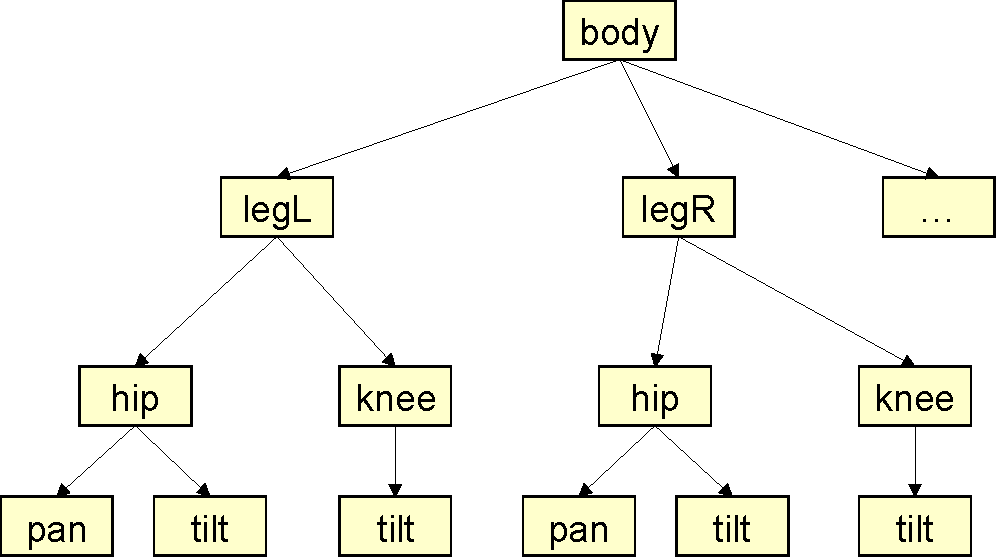
\includegraphics[width=.8\linewidth]{img/structure-tree}
\end{center}

The leaves of the tree are called \textit{devices}, and they usually
match physical devices in the robot: motors, sensors, lights, camera,
etc. Inside \urbi, the various objects corresponding to the tree
components are accessed by following the path of objects inclusions,
like in the example below (shortcuts will be described later):

\begin{urbifixme}
body.legR.hip.tilt;
body.legL.knee.led;
body.legL.hip;
// ...
\end{urbifixme}


The structure tree should not be mistaken for a representation of the
kinematics chain of the robot. The kinematics chain is built from a
subset of the devices corresponding to motor devices, and it
represents spatial connections between them. Except for these motor
devices, the structure tree components do not have a direct
counterpart in the kinematics chain, or, if they do, it is as a subset
of the kinematics chain (for example, \texttt{legR} is a subset of the
whole kinematics chain).


The goal of this standard is to provide guidelines on how to define
the components and the structure tree, knowing the kinematics chain of
the robot.

\section{Frame of Reference}

In many cases, it will be necessary to refer to an absolute frame of
reference attached to the robot body. To avoid ambiguities, the
standard frame of reference will have the following definition:

\begin{center}
  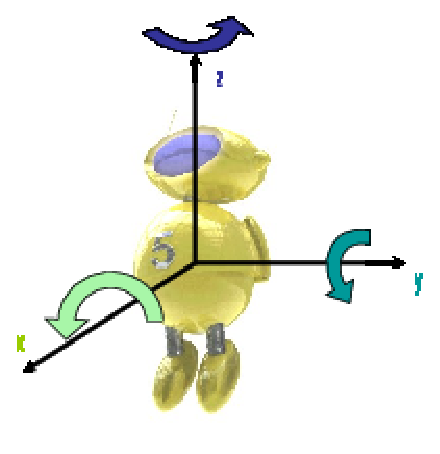
\includegraphics{img/reference-frame}
\end{center}

\begin{description}
\item[Origin] the center of mass of the robot
\item[X axis] oriented towards the front of the robot. If there is a
  camera, the front is defined by the default direction of the camera,
  otherwise the front will be seen as the natural frontal orientation
  for a mobile robot (the direction of “forward” movement). If the
  robot is not naturally oriented, the X axis will be chosen to match
  the main axis of symmetry of the robot body and it will be oriented
  towards the smallest side, typically the top of a cone for
  example. In case of a perfectly symmetrical body, the X axis can be
  chosen arbitrarily but a clear mark should be made visible on the
  robot body to indicate it.
\item[Z axis] oriented in the opposite direction from the gravity. If
  there is no gravity or natural up/down orientation in the
  environment or normal operation mode of the robot, the Z axis should
  be chosen in the direction of the main axis of symmetry in the
  orthogonal plane defined by the X axis, oriented towards the
  smallest side. In case of a perfectly symmetrical plane, the Z axis
  can be chosen arbitrarily but a clear mark should be made visible on
  the robot body to indicate it.
\item[Y axis] oriented to make a right-handed coordinate system.
\end{description}


The axes are oriented in a counter-clockwise direction, as depicted in
the illustration above.

\section{Component naming}

The name of a component A, which is a sub-component of component B, is
divided into two parts: the generic designation of a subpart of the
kinematics chain (like ‘leg’, ‘head’, ‘finger’) that A is referring
to, and optionally some topological disambiguator relative to its
position within the component B it belongs to. For example, when there
are two legs, we need to differentiate between the right and left leg,
relative to the body component they belong to. The first part is
called the \textit{designation}, and the second optional part is
called the \textit{localization}.

\paragraph{Designation}


The designation of a component is a usually robot-specific and depends
on the class of the robot (wheeled, humanoid, animaloid, etc). We will
give in the following chapters some guidelines for the most current
designations, and we will give more advanced rules for rare customized
cases.


The designation is the critical part of the naming standard. We cannot
possibly cover all future configurations and conceivable robot complex
bodies, but the current document will grow whenever we find a new
case.  We hope to be already covering most of the main cases you can
find in the industry.

\paragraph{Localization}

Localization is necessary when there are two identical sub-components
A1 and A2 belonging to the same component B, like for example two legs
or two arms attached to the main body. Usually this can be sorted out
with simple geometric qualifiers like \textit{Right/Center/Left},
\textit{Front/Middle/Back} or \textit{Up/In-between/Down}. The naming
convention is to use the first letter of the geometric characteristic,
like R for Right, I for In-between.  Note that “right” or “front” are
understood here from the point of view of a man standing and looking
in the direction of the X-axis of the robot, and \textit{Up/Down}
matches the Z-axis, as depicted in the figure below:

\begin{center}
  
\includegraphics[width=.5\linewidth]{img/cube}
\end{center}

Several geometric qualifiers can be used at the same time to further
refine the position. As a convention, side information comes first
(R/C/L), followed by the depth information (F/M/H) and then the height
information (U/I/D).

You can further qualify a side+depth localization with an additional
R/L side information. This can be used in the typical layout below:

\begin{center}
  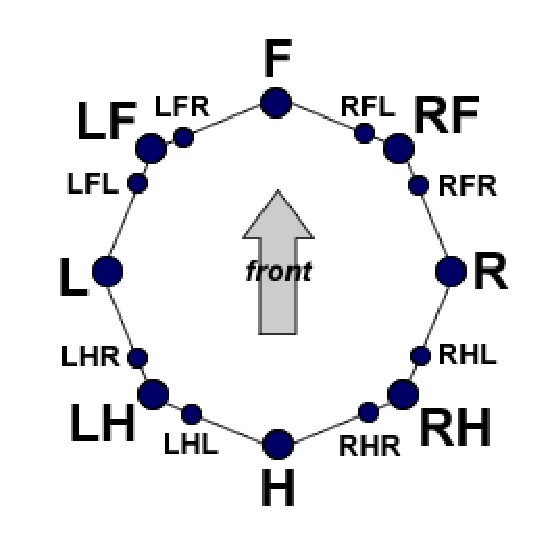
\includegraphics{img/lrfh}
\end{center}

This dual positioning using side+depth can also be used to combine
side+height or height+depth information.

Some layouts will typically imply a bilateral organization like for
example an insectoid robot with a series of 3 legs on both side of its
body. In that case, an array will be used and follow the geometrical
localization (R/L). The smaller the number, the closer to the front:
R[1], R[2], R[3] and L[1], L[2], L[3]. This can be used when there is
at least 3 components on each side, otherwise the
\textit{Front}/\textit{Back} approach prevails.

Some components like spines or tails are highly articulated with a set
of identical sub-components. When talking about these sub-components,
the above localization should be replaced by an array with a numbering
starting at 0. The smaller the number, the closer the sub-component is
to the robot main body. For surface-like sub-components, like skin
touch sensors, the array can be two dimensional.

Other possible localization for sensors are the X, Y and Z axis
themselves, like for example for an accelerometer or a gyro sensor,
available in each of the three directions.


Examples of component names including localization:

\begin{urbifixme}
legR, legL, armR, armL;
fingerR, fingerC, fingerL;      // three fingers hand
joint[0], joint[1] ... joint[5] // from tail
touch[478][124]                 // from skin
accelX, accelY, accelZ;         // typical accelerometer
gyroX, gyroY, gyroZ;            // typical gyro sensor
\end{urbifixme}

\section{Facets}

\urbi allows multiple inheritances between objects. This feature can be
used to introduce the notion of “facet”. A facet is an object in \urbi
that describes some aspect of a type of component.

For example, for a joint, we can have a “swivel” facet, used to define
patella joints. For the robot body itself, we have a “mobile” facet
describing mobile robots, which includes some standard way of
requesting a move forward, a turn, etc. A robot with a Pan/Tilt camera
or otherwise moving camera will have the “panoramic” facet which is
abstracting the way the robot can turn its gaze in any direction.

In short, facets are standard Urbi objects that components can inherit
from to acquire some functionalities, expressed as a standard
interface. We will describe in the following pages a few of the most
standard facets. Each facet should be reimplemented for any particular
robot that uses them, for example the “mobile” facet will have a
completely different implementation with a humanoid robot and a wheeled
robot.

\facet{identity}

Contains information about the robot identity.

\begin{slots}
  \slot{type}
  {
    This describes the robot category among: humanoid, fourlegged,
    wheeled, industrial arm. It gives a general idea of the robot
    family, but does not replace a more systematic probe of available
    services by investigating the list of attributes of the object.
  }

  \slot{name}%
  {%
    Name of the robot.%
  }

  \slot{model}%
  {%
    Model of the robot.%
  }

  \slot{serial}%
  {%
    Serial number (if available).%
  }

\end{slots}


\facet{network}

Contains information about the network identification of the robot.

\begin{slots}
  \slot{IP}%
  {%
    IP address of the robot.%
  }

  \slot{gateway}%
  {%
    Gateway IP address.%
  }

  \slot{latency}%
  {%
    Measured average network latency.%
  }

  \slot{bandwidth}%
  {%
    Measured average network bandwidth.%
  }

\end{slots}

\facet{motor}

This facet is used to describe a generic motor controller.

\begin{slots}
  \slot{val}%
  {%
    This slot is a generic pointer to a more specific slot describing
    the motor position, like \texttt{position} or \texttt{angle},
    depending on the type of motor. It is mandatory in the Urbi Ready
    standard as a universal proxy to control an actuator. The more
    specific slot is described in a subclass of \texttt{motor}.%
  }

  \optSlot{PGain}%
  {%
    Controls the P gain of the PID controller.%
  }

  \optSlot{IGain}%
  {%
    Controls the I gain of the PID controller.%
  }

  \optSlot{DGain}%
  {%
    Controls the D gain of the PID controller.%
  }

\end{slots}

\facet[motor]{linearMotor}


This facet is used to describe a linear motor controller.

\begin{slots}
  \slot{position}%
  {%
    Position of the motor in centimeters.  Pointed to by the
    \texttt{val} slot.%
  }

  \slot{force}%
  {%
    Intensity of the measured or estimated force applied on a linear
    motor.%
  }

\end{slots}

\facet[motor]{rotationalMotor}


This facet is used to describe a rotational motor controller.

\begin{slots}
  \slot{angle}%
  {%
    Angle of the motor in degree, modulo 360. Pointed to by the
    \texttt{val} slot.%
  }

  \slot{turn}%
  {%
    Absolute angular position of the motor, expressed in number of
    turns.%
  }

  \slot{torque}%
  {%
    Intensity of the measured or estimated torque applied on the
    motor.%
  }

\end{slots}


\facet{sensor}

This facet is used to describe a generic sensor.

\begin{slots}
  \slot{val}%
  {%
    This slot is a generic pointer to a more specific slot describing
    the sensor value, like \texttt{distance} or \texttt{temperature},
    depending on the type of sensor. It is mandatory in the Urbi Ready
    standard as a universal proxy to read a sensor. The more specific
    slot is described in a subclass of \texttt{sensor}.%
  }

\end{slots}


\facet[sensor]{distanceSensor}

This facet is used to describe a distance sensor (infrared, laser,
ultrasonic...).

\begin{slots}
  \slot{distance}%
  {%
    Measured distance expressed in meters.  Pointed to by the
    \texttt{val} slot.%
  }

\end{slots}


\facet[sensor]{touchSensor}

This facet is used to describe a touch pressure sensor (contact,
induction,...).

\begin{slots}
  \slot{pressure}%
  {%
    Intensity of the pressure put on the touch sensor. Can be 0/1 for
    simple buttons or expressed in Pascal units. Pointed to by the
    \texttt{val} slot.%
  }

\end{slots}


\facet[sensor]{accelerationSensor}

This facet is used to describe an accelerometer.

\begin{slots}
  \slot{acceleration}%
  {%
    Acceleration expressed in m/s2.  Pointed to by the \texttt{val}
    slot.%
  }

\end{slots}

\facet[sensor]{gyroSensor}
This facet is used to describe an gyrometer.

\begin{slots}
  \slot{acceleration}%
  {%
    Acceleration expressed in rad/s2.  Pointed to by the \texttt{val}
    slot.%
  }
\end{slots}

\facet[sensor]{temperatureSensor}
This facet is used to describe a temperature sensor.

\begin{slots}
  \slot{temperature}%
  {%
    Measured temperature in Celsius degrees.  Pointed to by the
    \texttt{val} slot.%
  }

\end{slots}

\facet{mobile}

Mobile robots all share this generic interface to provide high order
level motion control capabilities.

\begin{slots}
  \slot{go(x)}%
  {%
    Move approximatively x meters forward if x is positive, backward
    otherwise.%
  }

  \slot{turn(x)}%
  {%
    Turn right approximatively x degrees.  x can be a positive or
    negative value.%
  }

\end{slots}

\facet{tracker}

Camera-equipped robots can sometimes move the orientation of the field
of view horizontally and vertically, which is a very important feature
for many applications. In that case, this facet abstracts how such
motion can be achieved, whether it is done with a pan/tilt camera or
with whole body motion or a combination of both.

\begin{slots}
  \slot{yaw}%
  {%
    Rotational articulation around the Z axis in the robot, expressed
    in degrees.%
  }

  \slot{pitch}%
  {%
    Rotational articulation around the Y axis in the robot, expressed
    in degrees.%
  }

\end{slots}

\facet{videoin}

The videoin facet groups every information relative to cameras or any
image sensor.

\begin{slots}
  \slot{val}%
  {%
    Binary value corresponding to the image, expressed in the current
    unit (RGB, jpeg, YCrCb...). The unit can be changed like any other
    regular unit in Urbi. %
  }

  \slot{xfov}%
  {%
    The x Field Of View of the camera expressed in degrees.%
  }

  \slot{yfov}%
  {%
    The y Field Of View of the camera expressed in degrees.%
  }

  \slot{height}%
  {%
    Height of the image in the current resolution, expressed in
    pixels%
  }

  \slot{width}%
  {%
    Width of the image in the current resolution, expressed in pixels%
  }

  \optSlot{shutter}%
  {%
    The shutter speed (expressed in ms). 0 if non applicable.%
  }

  \optSlot{wb}%
  {%
    White balance (expressed with an integer value depending on the
    camera documentation). 0 if non applicable.%
  }

  \optSlot{gain}%
  {%
    Camera gain amplification (expressed as a coefficient between 0
    and infinity). 1 if non applicable.%
  }

  \optSlot{resolution}%
  {%
    Can be used to specify a given resolution, expressed as a
    percentage of the maximal resolution of the camera (number between
    0 and 1). 1 if non applicable.

    Once modified, the effective resolution in X/Y can be checked with
    the width and height slots.%
  }

\end{slots}

\facet{audioout}
The audioout facet groups every information relative to speakers.

\begin{slots}
  \slot{val}%
  {%
    The speaker value, expressed as a binary, in the format given by
    the binary header during the assignment.

    Speakers are write-only devices, so there is not much sense in
    reading the content of this attribute. At best, it returns the
    remaining sound to be played if it is not over yet, but this is
    not a requirement.%
  }

  \slot{remain}%
  {%
    The amount of time remaining to play in the speaker sound buffer
    (expressed in \textit{ms} as a default unit).%
  }

  \slot{playing}%
  {%
    This is a boolean value which is true when there is a sound
    currently playing (the buffer is not empty)%
  }

  \optSlot{volume}%
  {%
    Volume of the play back, in decibels.%
  }
\end{slots}



\facet{audioin}

The audioin facet groups every information relative to microphones.

\begin{slots}
  \slot{val}%
  {%
    Binary value corresponding to the sound heard, expressed in the
    current unit (wav, mp3...). The unit can be changed like any other
    regular unit in Urbi.

    The content is the sound heard by the microphone since the last
    update event.%
  }

  \slot{duration}%
  {%
    Amount of sound in the val attribute, expressed in \textit{ms}.%
  }

  \optSlot{gain}%
  {%
    Microphone gain amplification (expressed between 0 and 1)%
  }
\end{slots}


\facet{blobDetector}

Ball detectors, marker detectors and various feature-based detectors
should all share a similar interface. They extract a part of the image
that fits some criteria and define a “blob” accordingly. Here are the
typical slots expected:

\begin{slots}
  \slot{x}%
  {%
    The x position of the center of the blob in the image%
  }

  \slot{y}%
  {%
    The y position of the center of the blob in the image%
  }

  \slot{ratio}%
  {%
    The size of the blob expressed as a normalized image size: 1 =
    full image, 0 = nothing.%
  }

  \slot{visible}%
  {%
    A Boolean expressing whether there is a blob in the image or not
    (see threshold)%
  }

  \slot{threshold}%
  {%
    The minimum value of ratio to decide that the blob is visible.%
  }

  \optSlot{orientation}%
  {%
    Angle of the main ellipsoid axis of the blog (0 = horizontal),
    expressed in degrees.%
  }

  \optSlot{elongation}%
  {%
    Ratio between the main and the second diameter of the blob
    enveloping ellipse.%
  }

\end{slots}

\facet{textToSpeech}
Text to speech allows to read text using a speech synthetizor. Default
implementations should use the \texttt{speaker} component (or alias) as
their default sound output.

\begin{slots}
  \optSlot{lang}%
  {%
    The language used, in international notation (fr, en, it…): ISO
    639%
  }

  \optSlot{speed}%
  {%
    How fast the voice should go, between 0 and 1.%
  }

  \optSlot{pitch}%
  {%
    Voice pitch, between 0 and 1.%
  }

  \optSlot{gender}%
  {%
    Gender of the speaker (0:male/1:female)%
  }

  \optSlot{age}%
  {%
    Age of the speaker, if applicable%
  }

  \optSlot{name}%
  {%
    Most TTS engine will propose several voices, this attributes
    allows picking one. It’s a string identifier specific to the TTS
    developer.%
  }

  \slot{say(s)}%
  {%
    Speak the sentence given in parameter \var{s}.%
  }

  \optSlot{voicexml(s)}%
  {%
    Speak the text \var{s} expressed as a VoiceXML string.%
  }

  \optSlot{script(s)}%
  {%
    Speak the text \var{s} augmented by script markups (see specific
    Gostai documentation) to generate \urbi events.%
  }

\end{slots}


\facet{speechRecognizer}

Speech recognition allows to transform a stream of sound into a text
using various speech recognition algorithms. Default implementations
should use the \texttt{micro} component (or alias) as their default
sound input.

\begin{slots}
  \optSlot{lang}%
  {%
    The language used, in international notation (fr, en, it…): ISO
    639%
  }
\end{slots}

\begin{slots}[Events]
  \slot{hear(s)}%
  {%
    This event has one parameter which is the string describing what
    the speech engine has recognized (can be a word or a sentence).%
  }
\end{slots}

\section{Standard Components}

Standard components correspond to components typically found in wheeled
robots, humanoid or animaloid robots, or in industrial arms.


The table on the next pages summarize the currently referenced standard
components, with a description of potential components that they could
be subcomponent of, a description of potential components they may
contain, and a list of relevant facets. This table should be seen as a
quick reference guide to identify available components in a given
robot.

\paragraph{Yaw/Pitch/Roll orientation: guideline}

It is not always clear which rotational direction corresponds to the
yaw, pitch or roll components (listed in the table below). This is a
quick guideline to help determine the proper association.

Let us consider the robot in its resting, most prototypical position,
like “standing” on two or four legs for a humanoid or animaloid, and
let all members “naturally” fall under gravity. When gravity has no
effect on a certain joint (because it is in the orthogonal plan to Z,
for example), the medium position between rangemin and rangemax should
be used. The body position achieved will be considered as a reference.
Then for each component that is described in terms of yaw/pitch/roll
sub-decomposition, the association will be as follow:

\begin{description}
\item[yaw] rotational articulation around the Z axis in the robot.
\item[pitch] rotational articulation around the Y axis in the robot.
\item[roll] rotational articulation around the X axis in the robot.
\end{description}

When there is no exact match with the X/Y/Z axis, the closest match, or
the default remaining available axis, should be selected to determine
the yaw/pitch/roll meaning.

\bigskip

\newcommand{\component}[5]
{
  \lstindex{#1} &
  #5 &
  \code{#2} &
  \code{#3} &
  \code{#4}\\\hline
}

\tablehead{\hline
\textbf{Name} &
\textbf{Description} &
\textbf{Sub. of} &
\textbf{Contains} &
\textbf{Facets} \\\hline}
\begin{supertabular}{|m{.115\linewidth}|m{.45\linewidth}|*{4}{m{.12\linewidth}|}}
  \component{robot}{-}{body}{identity network mobile tracker}{
    %%
    This is the main component that represents an abstraction of the
    robot.
    %%
  }

  \component{body}{robot}{arm leg neck head wheel tail skin torso
    \ldots}{-}{
    %%
    This is the main component that contains every piece of hardware
    in the robot. This includes all primary kinematics sub-chains
    (arms, legs, neck, head, etc) and non-localized sensor arrays,
    typically body skin or heat detectors.  Localized sensors, like
    fingertips touch sensors, will typically be found attached to the
    finger component they belong and not directly to the body.
    %%
  }

  \component{leg}{body}{hip knee ankle foot joint}{-}{
    %%
    Legs are found in humanoid or animaloid robots and correspond to
    part of the kinematics chain that are attached to the main body by
    one extremity only and which do touch the ground in normal
    operation mode (unlike arms). A typical configuration for
    humanoids contains a hip, a knee and an ankle. If the leg is more
    segmented, the leg can be described with a simple array of joints.
    %%
  }

  \component{arm}{body}{shoulder elbow wrist hand grip  joint}{-}{
    %%
    Unlike legs, an arm’s extremity does not always touch the ground
    in normal operating mode. This applies to humanoid robots or
    single-arm industrial robots. Arms supersede legs in the
    nomenclature: if a body part behaves alternatively like an arm and
    like a leg, it will be considered as an arm.
    %%
  }

  \component{shoulder}{arm}{yaw pitch roll}{-}{
    %%
    The shoulder is the upper part of the arm. It can have one, two or
    three degrees of freedom and is the closest part of the arm
    relative to the body.
    %%
  }

  \component{elbow}{arm}{pitch}{-}{
    %%
    Separates the upper arm and the lower arm, this is usually a
    single rotational axis.
    %%
  }

  \component{wrist}{arm}{yaw pitch roll}{-}{
    %%
    Connects the hand and the lower part of the arm. Usually three
    degrees of freedom axis.
    %%
  }

  \component{hand}{arm}{finger}{-}{
    %%
    The hand is an extension of the arm that usually holds
    fingers. It’s not the wrist, which is articulated and between the
    arm and the hand.
    %%
  }

  \component{finger}{hand}{touch}{motor}{
    %%
    Fingers are a series of articulated motors at the extremity of the
    arm, and connected to the hand. They are usually localized with
    arrays and/or lateral localization respective to the hand.
    %%
  }

  \component{grip}{arm hand}{touch}{motor}{
    %%
    Simple two-fingers system.
    %%
  }

  \component{hip}{leg}{yaw pitch roll}{-}{
    %%
    The hip is the upper part of the leg and connects it to the main
    body. It can have one, two or three degrees of freedom.
    %%
  }

  \component{knee}{leg}{pitch}{-}{
    %%
    Separates the upper leg and the lower leg, this is usually a
    single rotational axis.
    %%
    }

  \component{ankle}{leg}{yaw pitch roll}{-}{
    %%
    Connects the foot and the lower part of the leg. Usually three
    degrees of freedom axis.
    %%
    }

  \component{foot}{leg}{touch}{-}{
    %%
    The foot is an extension of the leg that usually holds toes. It’s
    not the ankle, which is articulated and between the leg and the
    foot. The foot can also contain touch sensors in simple
    configurations.
    %%
  }

  \component{toe}{foot}{touch}{motor}{
    %%
    Like fingers, but attached to the foot.
    %%
  }

  \component{neck}{body}{yaw pitch roll}{-}{
    %%
    The neck corresponds to a degree of freedom not part of the head,
    but relative to the rigid connection between the head and the main
    body.
    %%
  }

  \component{tail}{body}{joint}{-}{
    %%
    A tail is a series of articulated motors at the back of the robot.
    %%
  }

  \component{head}{body neck}{camera mouth ear lip eye eyebrow}{-}{
    %%
    The head main pivotal axis.
    %%
  }

  \component{mouth}{head}{lip}{motor}{
    %%
    The robot mouth (open/close)
    %%
  }

  \component{ear}{head}{-}{motor}{
    %%
    Ears may have degrees of freedom in
    certain robots.
    %%
  }

  \component{joint}{tail arm leg lip}{-}{motor}{
    %%
    Generic articulation in the robot.
    %%
  }

  \component{yaw}{neck knee ankle shoulder elbow wrist
    torso}{-}{rotational\-Motor}{
    %%
    Rotational articulation around the Z axis in the
    robot. \textit{See the introduction paragraph on yaw/pitch/roll
      orientation for more details on how to identify which direction
      corresponds to yaw.}
    %%
  }

  \component{pitch}{neck knee ankle shoulder elbow wrist
    torso}{-}{rotational\-Motor}{
    %%
    Rotational articulation around the Y axis in the
    robot. \textit{See the introduction paragraph on yaw/pitch/roll
      orientation for more details on how to identify which direction
      corresponds to pitch.}
    %%
  }

  \component{roll}{neck knee ankle shoulder elbow wrist
    torso}{-}{rotational\-Motor}{
    %%
    Rotational articulation around the X axis in the
    robot. \textit{See the introduction paragraph on yaw/pitch/roll
      orientation for more details on how to identify which direction
      corresponds to roll.}
    %%
  }

  \component{lip}{mouth}{joint}{motor}{
    %%
    Corresponds to animated lips.
    %%
  }

  \component{eye}{head}{camera}{-}{
    %%
    Corresponds to the eyeball pivotal axis.
    %%
    }

  \component{eyebrow}{head}{joint}{motor}{
    %%
    Some robots will have eyebrow with generally one or several degree
    of freedom.
    %%
    }

  \component{torso}{body}{yaw pitch roll}{-}{
    %%
    This corresponds to a pivotal or rotational axis in the middle of
    the main body.
    %%
    }

  \component{spine}{torso}{joint}{-}{
    %%
    This is a more elaborated version of “torso”, with a series of
    articulations to give several degrees of freedom in the back of
    the robot.
    %%
    }

  \component{clavicle}{body}{-}{motor}{
    %%
    This is not to be mixed up with the “top of the arm” body part. It
    is an independent degree of freedom that can be used to bring the
    two arms closer in a sort of “shoulder raising” movement.
    %%
    }

  \component{touch}{finger grip foot toe}{-}{touchSensor}{
    %%
      Touch sensor.
    %%
    }

  \component{gyro}{body}{-}{gyroSensor}{
    %%
      Gyrometer sensor.
    %%
    }

  \component{accel}{body}{-}{accel\-eration\-Sensor}{
    %%
      Accelerometer sensor.
    %%
    }

  \component{camera}{head body}{-}{videoin}{
    %%
    Camera sensor. If several cameras are available, localization
    shall apply, however there must always be an alias from
    \texttt{camera} to one of the effective camera (like
    \texttt{cameraR} or \texttt{cameraL}).
    %%
    }

  \component{speaker}{head body}{-}{audioin}{
    %%
    Speaker device. If several speakers are available, localization
    shall apply, however there must always be an alias from
    \texttt{speaker} to one of the effective speakers (like
    \texttt{speakerR} or \texttt{speakerL}).
    %%
    }

  \component{micro}{head body}{-}{audioout}{
    %%
    Microphone devices. If several microphones are available,
    localization shall apply, however there must always be an alias
    from \texttt{micro} to one of the effective microphones (like
    \texttt{microR} or \texttt{microL}).
    %%
  }

  \component{speech}{robot}{-}{speech\-Recognizer}{
    %%
      Speech recognition component.
    %%
    }

  \component{voice}{robot}{-}{textTo\-Speech}{
    %%
      Voice synthesis component.
    %%
    }

\end{supertabular}



\section{Compact notation}

Components are usually identified with their full-length name, which is
the path to access them inside the structure tree. For convenience and
backward compatibility with pre-2.0 versions of \urbi, there is also a
compact notation available. We will describe here how to construct the
compact notation starting from the full name and the structure tree.

\tablehead{\hline
Full name &
Compact name\\\hline}
\begin{supertabular}{|m{9.008cm}|m{5.533cm}|}
\code{robot.body.armR.elbow} &
\code{elbowR} \\\hline
\code{robot.body.head.yaw} &
\code{headYaw} \\\hline
\code{robot.body.legL.knee.pitch} &
\code{kneeL} \\\hline
\code{robot.body.armR.hand.finger[3][2]} &
\code{fingerR[3][2]} \\\hline
\code{robot.body.armL.hand.fingerR} &
\code{fingerLR} \\\hline
\end{supertabular}

The rule is to move every localization qualifier at the end of the
compact notation, in the order where they appear in the full-length
name. The remaining component names should then be considered one by
one to see if they are needed to remove ambiguities. If they are not,
like typically the robot or body components which are shared with
almost every other full-length name, they can be ignored. If finally
several component names have to be kept, they should be separated by
using upper case letters for the first character instead of a dot, like
in Java-style notation.

\begin{example}[\texttt{robot.body.armL.hand.fingerR}]~\\
  \begin{enumerate}
  \item Move all localization at the end:
    \texttt{robot.body.arm.hand.fingerLR}
  \item The fullname remaining is: \texttt{robot.body.arm.hand.finger}
  \item \texttt{finger} should be kept, \texttt{hand}, \texttt{arm},
    \texttt{body} and \texttt{robot} are not necessary since every
    finger component will always be attached only to a hand, itself
    attached to an arm and a body and a robot.
  \item The result is \texttt{fingerLR}
  \end{enumerate}
\end{example}


\begin{example}[\texttt{robot.body.head.yaw}]~\\
  \begin{enumerate}
  \item No localization to move
  \item \texttt{yaw} must be kept because \texttt{head} also have a
    \texttt{pitch} subcomponent and
  \item \texttt{head} must also be kept to avoid ambiguity with other
    components having a \texttt{yaw} subcomponent.
  \item The result is \texttt{headYaw}
  \end{enumerate}
\end{example}

\begin{example}[\texttt{robot.body.legL.knee.pitch}]~\\
  \begin{enumerate}
  \item Move all localization at the end:
    \texttt{robot.body.leg.knee.pitchL}
  \item \texttt{pitch} is not necessary because \texttt{knee} has only a
    \texttt{pitch}, so \texttt{knee} will be kept only
  \item The result is \texttt{kneeL}
  \end{enumerate}
\end{example}


%%% Local Variables:
%%% mode: latex
%%% TeX-master: "../urbi-sdk"
%%% End:


%%% Local Variables:
%%% coding: utf-8
%%% mode: latex
%%% TeX-master: "../urbi-sdk"
%%% ispell-dictionary: "american"
%%% ispell-personal-dictionary: "../urbi.dict"
%%% fill-column: 76
%%% End:

%% Copyright (C) 2010, Gostai S.A.S.
%%
%% This software is provided "as is" without warranty of any kind,
%% either expressed or implied, including but not limited to the
%% implied warranties of fitness for a particular purpose.
%%
%% See the LICENSE file for more information.

\section{UObject}

UObject is used by the \lstinline|UObject| API (see
\autoref{part:uobject}) to represent a bound \Cxx instance.

All the UObjects are copied under an unique name as slots of
\lstinline{uobjects}.

\subsection{Prototypes}
\begin{refObjects}
\item[Object]
\end{refObjects}

\subsection{Slots}

\begin{urbiscriptapi}
\item[__uobjectName]%
  Unique name assigned to this object. This is also the slot name of
  \refSlot[Global]{uobjects} containing this \lstinline|UObject|.
\end{urbiscriptapi}

%%% Local Variables:
%%% mode: latex
%%% TeX-master: "../urbi-sdk"
%%% ispell-dictionary: "american"
%%% ispell-personal-dictionary: "../urbi.dict"
%%% fill-column: 76
%%% End:


\part{References and Index}

\phantomsection % otherwise hyperlinks to previous chapter.
\addcontentsline{toc}{chapter}{\indexname}
\printindex


\end{document}

% printing, operators, waituntil

% LocalWords:  Urbi monomethods netcat cosinus timestamp subscopes subscope lst
% LocalWords:  getSlot setSlot updateSlot slotNames removeSlot uid arg ok ko ss
% LocalWords:  elt baz quux FIXME getslot lookup protos proto addProto asString
% LocalWords:  removeProto locateSlot locateslot lhs evalArgAt evalArgs ary
% LocalWords:  mytag timeOut myEvent
